\documentclass[11pt,fleqn]{book}

\usepackage{shorttoc}
\usepackage{makeidx,natbib,vmargin,setspace}
\usepackage{tabu}

\usepackage{color}
\usepackage{framed}

\usepackage{amsfonts}
\usepackage{amssymb, amsthm}

%\usepackage{txfonts, mathtools}
%\usepackage{libertine}
\usepackage[T1]{fontenc}

%\usepackage[T1]{fontenc}
%\usepackage{stix}

\usepackage[colorlinks=true, pdfstartview=FitV, citecolor=blue!50!black, linkcolor=red!30!black]{hyperref}

\usepackage{graphicx,graphics,tikz}
\usepackage{microtype}
%\usepackage{url}

\usepackage{eqnarray}
\usepackage{rotating}
\usepackage{booktabs}
\usepackage{setspace}
\usepackage{dcolumn}

\usepackage{mathtools}
\usepackage{amsmath}
\usepackage{graphicx}
\usepackage{float}
\restylefloat{table}
\usepackage[section]{placeins}

\usepackage{fancyhdr}
\pagestyle{fancy}
\renewcommand{\chaptermark}[1]{\markboth{#1}{}}
\renewcommand{\sectionmark}[1]{\markright{\thesection\ #1}}
\fancyhf{}
\fancyhead[LE,RO]{\bfseries\thepage}
\fancyhead[LO]{\bfseries\rightmark}
\fancyhead[RE]{\bfseries\leftmark}
\renewcommand{\headrulewidth}{0.5pt}
\renewcommand{\footrulewidth}{0pt}
\addtolength{\headheight}{0.5pt}
\setlength{\footskip}{0in}
\renewcommand{\footruleskip}{0pt}
\fancypagestyle{plain}{%
\fancyhead{}
\renewcommand{\headrulewidth}{0pt}
}
\parskip 0.05in

\usepackage{appendix}
\usepackage{chngcntr}
\usepackage{etoolbox}

\AtBeginEnvironment{subappendices}{%
\chapter*{Appendix for Chapter~\thechapter}
\addcontentsline{toc}{chapter}{Appendices}
\counterwithin{figure}{section}
\counterwithin{table}{section}
}

\DeclarePairedDelimiter\abs{\lvert}{\rvert}%
\DeclarePairedDelimiter\norm{\lVert}{\rVert}%

\makeatletter
\let\oldabs\abs
\def\abs{\@ifstar{\oldabs}{\oldabs*}}
%
\let\oldnorm\norm
\def\norm{\@ifstar{\oldnorm}{\oldnorm*}}
\makeatother


\newcounter{llst}
\newenvironment{abet}{\begin{list}{\rm (\alph{llst})}{\usecounter{llst}
\setlength{\itemindent}{0em} \setlength{\leftmargin}{3em}
\setlength{\labelwidth}{2em} \setlength{\labelsep}{1em}}}{\end{list}}
\newenvironment{numm}{\begin{list}{\rm (\roman{llst})}{\usecounter{llst}
\setlength{\itemindent}{0em} \setlength{\leftmargin}{3.5em}
\setlength{\labelwidth}{2.5em} \setlength{\labelsep}{1em}}}{\end{list}}

\renewcommand{\baselinestretch}{1.25}

\newtheorem{thm}{Theorem}
\newtheorem{theorem}{Theorem}[section]
\newtheorem{acknowledgement}[theorem]{Acknowledgement}
\newtheorem{algorithm}[theorem]{Algorithm}
\newtheorem{axiom}[theorem]{Axiom}
\newtheorem{case}[theorem]{Case}
\newtheorem{claim}[theorem]{Claim}
\newtheorem{conclusion}[theorem]{Conclusion}
\newtheorem{condition}[theorem]{Condition}
\newtheorem{conjecture}[theorem]{Conjecture}
\newtheorem{corollary}[theorem]{Corollary}
\newtheorem{criterion}[theorem]{Criterion}
\newtheorem{definition}[theorem]{Definition}
\newtheorem{expl}[theorem]{Example}
\newtheorem{exercise}[theorem]{Exercise}
\newtheorem{hypothesis}[theorem]{Hypothesis}
\newtheorem{lemma}[theorem]{Lemma}
\newtheorem{notation}[theorem]{Notation}
\newtheorem{problem}[theorem]{Problem}
\newtheorem{proposition}[theorem]{Proposition}
\newtheorem{property}[theorem]{Properties}
\newtheorem{rmrk}[theorem]{Remark}
\newtheorem{solution}[theorem]{Solution}
\newtheorem{summary}[theorem]{Summary}
\newenvironment{proof}[1][Proof]{\noindent \textbf{#1.} }{\hfill
\rule{0.5em}{0.5em}}

\newenvironment{example}{\begin{expl} \rm}{\hfill $\blacklozenge$ \end{expl}}{}
\newenvironment{remark}{\begin{rmrk} \rm}{\hfill $\blacklozenge$ \end{rmrk}}{}

%\setpapersize{A4}
% \setmarginsrb{84pt}{64pt}{84pt}{72pt}{12pt}{10pt}{12pt}{30pt}

\makeindex

\begin{document}

\pagenumbering{roman}
\begin{titlepage}
    \begin{center}
        \vspace*{1cm}
        
        \huge
        \textbf{The Wealth of Networks}
        
        \vspace{0.5cm}
        \LARGE
        Entrepreneurship and the Entrepreneurial Function in Socially Structured Economies
        
        \vspace{1.5cm}
        
        \Large
        \textbf{Owen Sims}
        
        \vfill
        
        \large
        A thesis presented for the degree of\\
        Doctor of Philosophy
        
        \vspace{0.8cm}
        
        
\includegraphics[width=0.15\textwidth]{imgs/qublogo2.png}
        
        \large
        Queen's Management School\\
        Queen's University Belfast\\
        \today
        
    \end{center}
\end{titlepage}

\vspace*{\stretch{3}}

\thispagestyle{empty}

\newpage

\chapter*{Acknowledgements}

The research presented in this monograph has been financially supported by the Department of Learning and Employment (DEL) Northern Ireland. I gratefully acknowledge and appreciate this financial support from DEL and the possibilities to participate in presentations and conferences that Queen's University Belfast has given me for the last four years.

This research has been conducted in the Economics Department of Queen's Management School at Queen's University Belfast, Northern Ireland. I am thankful for all the many beneficial and encouraging discussions with members of our group over my academic career. 

I would like to thank my Masters and PhD supervisor Robert Gilles whose innovative ideas and love for the discipline inspired me throughout the process. He has given me much guidance and encouragement as both a mentor and friend throughout the years. To this I would also like to thank my secondary PhD supervisor, Graham Brownlow, who, since I began as a University student, has given me much advice.

Finally, thanks and love to my parents for putting up with me and continually pressuring me to finally finish writing this monograph. Without their support I would never finished writing.

\newpage

\setcounter{page}{1} \pagenumbering{roman}

\begin{singlespace}
\setcounter{tocdepth}{2}
\tableofcontents

\listoffigures

\chapter*{Abstract}

\addcontentsline{toc}{chapter}{Abstract}

Many academic economists and practitioners have recognised the need for a pragmatic reform of the economics discipline, particularly since the effects of the 2008 global financial crisis \citep{Hodgson2009}. Further, many also recognise the requirement for a cohesive perspective on issues regarding the entrepreneur and entrepreneurship within a micro- and macroeconomic perspective. We address---and provide a partial resolve to---both issues. In doing so we provide an insight into the methodological basis of a relational perspective of social and economic activity through the structure and evolution of the social division of labour propagated by the actions of entrepreneurs. Of specific interest is the emergence of new specialisations, institutional modification, and the exploitation of positional power by entrepreneurial leaders.

The theoretical development of the relational perspective is founded on a number of axioms and hypotheses derived from observations in economics, sociology, psychology, and evolutionary anthropology. From this, we elaborate, in a formal manner, on the inherent sociality of the individual economic agent and the production possibilities that are subjected to increasing returns to specialisation. This structure of each individuals' production set informs a set of professions, or socio-economic roles, that become embedded within the institutional fabric of society. Interaction infrastructures form as a consequence of the social and economic interaction between economic agents.

The formation interaction infrastructures lead to an uneven distribution of positional power within the matrix of relationships. Unique positional attributes of economic agents are reflected in entrepreneurial action and the exploitation of power in connecting, and potentially disconnecting, otherwise unconnected agents and communities. We investigate entrepreneurship in this way---through an institutional and topological perspective. Specifically, entrepreneurship motivates the evolution of the division of labour through the formation of new socio-economic roles; this, in turn, suggests an alteration of networked institutional infrastructure and the formation of unique positions in the matrix occupied by entrepreneurs.

Throughout the monograph, we claim that entrepreneurs are analogous to \emph{middlemen}. This is investigated further in a formal manner. We develop a set of tools to investigate the positional power of middlemen and apply these measures to situations of entrepreneurial activity. Our empirical applications include the elite Florentine marriage network of Renaissance Florence and the interlocking directorate network of New York City during the early twentieth Century.

\end{singlespace}

\newpage

\setcounter{page}{1} \pagenumbering{arabic}
\chapter{Introduction}

This monograph presents theoretical and empirical considerations in the field of entrepreneurship. The fundamental idea is that the act of entrepreneurship expresses a crucial development of the social division of labour; a phenomenon explicitly addressed during the 18th century. We specifically recall the work of Adam~\citet{Smith1776} who, in his discussion on the generation of economic wealth, places the operation and evolution of the division of labour at the forefront. Although Smith focusses on the economic activities of society from a dynamic point of view, his concept of the \emph{invisible hand}---and the theory that an economy is normally in some naturally \emph{stable state}---has dominated theoretical discourse. Over the last two centuries the dynamic concept of economic interaction that Smith sought to discuss in the \emph{Wealth of Nations} has been substituted for a more static analysis, and the importance that he placed on increasing returns to specialisation and the operation of the division of labour has been diluted. This is reflected in general equilibrium analysis, a cornerstone of traditional economic theory. The result of this analysis states that if there exists no government interference within the economic activities of individual agents then these activities bring about a stable situation that can be valued as a natural equilibrium in the economy.

The arrival of an economic system to a well-defined predetermined steady state, as expressed in general equilibrium modelling, contradicts the notion of active entrepreneurship. The act of entrepreneurship is a dynamic force that cannot emerge from a static economic steady state, as defined by general equilibrium theory; this is a perspective that is shared with more heterodox economic writers such as~\citet{Schumpeter1942}. As a consequence, the notion of the entrepreneur and the act of entrepreneurship lacks definition and application in traditional economic theory. The most compelling definitions of entrepreneurship emerge within more heterodox strands of economics and sociology, which subsequently lack an elaborate theoretical basis. The outcome is a shallow insight into the environmental context of entrepreneurship and the result that entrepreneurship has on the organisation and distribution of power within society.

The theory developed in this monograph expresses the importance of institutional structures and the organisation of trade to the process of entrepreneurship. We value the general equilibrium concept as an expression of a specific and efficient form of organisation of the trade processes in the economy. The assumptions enforced by the Walrasian model lead to the formation of a market whereby the axiom of perfectly competitive behaviour is expressed. The institutional structure is inflexible and the resulting organisation of society is perfectly formed, thus allowing no role for entrepreneurial actions. A more general way to consider the organisation of trade processes is through the perspective of a network, which emerges as a consequence of a pattern of exchanges between a population of agents under a given institutional system of governance and mechanism of trade. Under the Walrasian model of general equilibrium, a complete network emerges representing perfectly efficient market processes. In reality, networked markets are imperfectly connected; structural holes and opportunities for brokerage exist. These structural imperfections provide opportunities for entrepreneurial actors to exploit.

Throughout this monograph we propose other forms of organisation and trade processes in the economy, such as markets with imperfect structure, costly interactions, and heterogeneous positions of economic agents that derive from specialisation and the social division of labour. We establish a fundamentally dynamic theory of the economy, thus allowing for the development of entrepreneurship in a natural way. This is the purpose of our initial theorising; it regards how we perceive the interaction space of the economy and allows us to appropriately define the entrepreneur and act of entrepreneurship. From this, we can analyse entrepreneurial action and power within the context of empirical examples. Overall, we feel that this provides a better description of how real-world economic processes take place. 

The monograph is divided into three parts; each of which discusses certain modelling aspects of the economy under different forms of trade organisation, socio-economic states and entrepreneurial activities. In this introductory chapter, we propose the notion of a socially structured economy, our perception of conventional modelling techniques under the Arrow-Debreu model, an introduction to the division of labour and a background into the theory of networked social structure and economic interactions.

\section{Aim of the monograph}
\label{sec:aaimOfMonograph}

Traditional economic theory is founded on the basis of \emph{methodological individualism}, \emph{methodological instrumentalism} and \emph{equilibration}. With methodological individualism, the individual decision-making agent has a central position in the theory. In most cases, an economy is described as a configuration of such individual economic agents, each of which attempts to optimise some well-defined pre-determined goal or objective. In this configuration it is assumed that the economic agent possesses the tools to optimise their utility; this is the crux of methodological instrumentalism \citep{Arnsperger2006}. This implies that economic decision processes in the economy are determined by the individual decision behaviour of these economic agents and by the configuration in which these economic agents are located. The outcome of this interaction is an equilibrium state represented as an organisational steady state. The economic system transitions from one steady state to another through some exogenous shock; suggesting that any dynamism is purely transitory and is fundamentally ill-defined---a \emph{manna from heaven}.

An additional assumption is that the individual economic agent can be described entirely with the use of individual attributes only. Examples of these individual attributes are an endowment bundle of commodities, individual production capacities and an individual preference relation on the set of well-defined, achievable commodity bundles for the particular economic agent. An illustration of this reliance on methodological individualism is with respect to the traditional Arrow-Debreu model of a perfectly competitive market system. This model contains a population of individual economic agents partitioned into a set of consumers and a set of producers. Consumers attempt to optimise a certain individual preference relation over the collection of achievable commodity bundles, while producers try to maximise their profit given their individual production capacities. These economic agents are placed within the context of a system of perfectly competitive markets, which puts certain constraints on the abilities of agents. The major constraint is given by the price levels determined by the market. Consumers limit themselves in terms of budget sets and, while producers adapt their production plan to maximise their profits. There is no consideration for other socially constructed characteristics that have an influence on the preferences and abilities of the individual decision-maker: the price level is the only `social' aspect that has a considerable influence on the population of individuals.

Within this context, the application of methodological individualism is very specific. Only individual decision-makers are participating in the processes that take place within the economy. Its use suggests that economic agents are essentially individuals who are interacting with each other according to the exogenous rules of the economic organisation and not with each other as a primitive social characteristic in their behaviour. This illustrates that the traditional method of microeconomic theorising implicitly involves a certain requirement on the `rules of the game'. 

In this monograph, we recognise that the rules of the game---which are reflected in the social and economic structure of the economy---are crucial in the design of a descriptive model of social and economic processes in that economy. Indeed, all economies are \emph{socially structured}; they are characterised by the socially constructed institutions and systems of governance that in turn guide the actions of a population of interconnected and interdependent agents. This social structure is flexible and, as such, is enforced and manipulated by economic agents themselves. This suggests that economic agents are not just individual decision-makers, but are decision-makers within a certain organisational environment consisting of a social and economic interaction architecture and behaviouristic conventions. An economic agent is still considered to be a decision-maker with some individual objective goal, but is also explicitly considered within some organisational environment determined by a well-defined governance system. The fact that an agent is considered as embedded within an organisational environment, leads to the acceptance of certain so-called \emph{social constraints} on the behaviour of that economic agent. Specifically, the agent's activity is contained within a matrix of interactions thus suggesting that the structure of interactions can also impose a constraint to their decision-making. We claim that constraints for some agents provide opportunities for others; distinctively, imperfections within society can provide opportunities for entrepreneurial activity.

\medskip\noindent \citet[p.~5]{Gilles1990} notes that the Arrow-Debreu model shows that objective market price expresses a specific form of aggregation---\emph{Walrasian aggregation}---which is a hypothesis of the organisation as represented by the market. Within the model, the price is representing the aggregation of demand and supply within the organisation of a perfectly competitive market. As a consequence, all agents communicate with each other through the market price only and not with each other directly. \citet{GillesDiamantaras2003} notes that this leads to a puzzle based on cyclical logic. But it more fundamentally suggests the inflexibility of perfect competition as an extremely efficient market structure. It is based on individualistic and symmetric economic agents that react to signals from market prices. The result is an equilibrium with no endogenous deviation and therefore has no capacity for wealth generation through entrepreneurial means. There are no deeper social features and attributes that influence the behaviour of the agents which shows that the functioning of the market is not influenced by other factors other than the market price.

The Arrow-Debreu model expresses a socially structured economy, albeit in a limited sense. The interactions of a finite set of individualistic decision-makers generate an idealistic market characterised by an objective price level for the exchange of a good. The socio-economic structure developed here is limited in the sense that it results in a static market mechanism shorn of all other social influences. In the real world, prices are not objective as in Arrow-Debreu style general equilibrium modelling. The notion of perfect competition is purely \emph{idealised}. Market imperfections, bounded human rationality, institutional structures and incomplete network architectures explain disparity and subjectivity in price levels. \citet{Blume2009} provide a model of exchange on a network based on the notion of Nash equilibrium. The model suggests that agents possessing dominant positions within a network of relations can influence price levels exposed to both producers and consumers. Institutions and socially constructed customs and cultures inform preferences and thus price levels within markets. We embrace these fundamentally social aspects of the economy within our modelling.

\subsection{Objectives}

The overall aim of the monograph is to provide a theory of entrepreneurship and the entrepreneurial function within socially structured economies. Our first objective in achieving this is to develop a perspective of embedded economic activity based on a population of specialised economic agents that form a functional social division of labour. The deepening of the social division of labour leads to a generation of wealth that benefits society as a whole. Specifically, we take a \emph{relational perspective} in which to view the foundations of social and economic phenomena. This foundation, established in Chapter~\ref{ch:relationalperspective}, provides a theory of social and economic interaction based on the use of socially embedded systems of governance which are successfully utilised given a foundation of trust. The relational perspective developed embraces Smith, yet deviates substantially from the traditional paradigm of the economics discipline founded on the Arrow-Debreu model.

The second objective is to explain and illustrate the role of the entrepreneur within the relational perspective and highlight the impact that entrepreneurship has on the evolution of the social division of labour, and therefore the development or, in some instances, the regression of the economy. Within our theory we note that the entrepreneur can have an impact on different dimensions of the economy: specifically impacting economic agents themselves, the economic interaction networks, and the institutions of the interaction environment.

The third objective is to provide a distinction between the act of entrepreneurship and the entrepreneurial function of the economy. The latter relates to the adaptive and creative act that many economic agents perform in producing outputs; this facilitates differentiation and great economic wealth, but not necessarily a new species of work or profession. The former relates to incredibly creative and disruptive acts that are reflective in the organisation of society and the interaction of new specialisations.

The final objective is to complement our theoretical discussion of the relational perspective and entrepreneurship with empirical analyses of entrepreneurial activities. This involves creating a set of tools that allows us to analyse data in a pragmatic way. From these tools, we can identify influential positions and activities within a networked economy. Our two main empirical applications are relate to the network of elite Florentine families and the directorate network of New York City during the beginning on the 20th century.

\medskip\noindent In developing a relational perspective of socio-economic activity we first provide a detailed insight into our central unit of analysis: the human agent. We investigate the micro-foundational elements of the human agent; elaborating on the agents' innate ability to form social relationships. We stress the co-evolution of the human brain with the growth of the increasingly complex social environment that it must navigate and organise. In doing so, we align our analysis with the hypothesis that the human brain has not developed in order to understand informational attributes of our environment but, converse to the conventional wisdom, our brains still remain imperfect in understanding environmental information. The economic decisions we make in complex situations are only made on the basis of bounded rationality, with informational constraints, and in situations of uncertainty.

Our characterisation of the economic agent relaxes two important assumptions of traditional economic modelling. The first is that there exists a dichotomy between consumers and producers: the population of economic agents is partitioned into two non-intersecting sets, each of which interact between, but not within, one another. The second refers to the structure of production possibilities, which do not lend themselves to Smith's notion of increasing returns to specialisation. As a consequence, specialised producers do not emerge naturally within the Walrasian framework. In modelling economic agents, we allow for increasing returns to specialisation through learning, which stands in contrast to the Arrow-Debreu model and other general equilibrium models developed from its foundation.

From this perspective of the human actor, and the society in which she is embedded, we elaborate on a theory that takes a topological analysis of social and economic interactions through the evolution of institutions that facilitate exchange and the deepening of the division of labour. We suggest that the division of labour naturally leads to the formation of relational networks, and from this we investigate the evolution of these relational networks---and thus the evolution of the economy---through the perspective of the entrepreneurial function, which primarily acts to extend the division of labour. As such we contend that the evolution of the socio-economic networks, and the systems of governance that hold them together, can only be explained through the use of the entrepreneurial function and the subsequent extension, or contraction, of the social division of labour.

\subsection{Motivation}

The development of a novel model for investigating socio-economic phenomena has come from two overlapping concerns. The first is prompted by the apparent deficiency in mainstream theory to convincingly address the emergence of new organisational structures and technologies and to fully incorporate the entrepreneurial function within the economy. The entrepreneur is left undeveloped in many formal economic theories. The main problem of these mainstream theories lies in appropriately modelling the entrepreneurial function derives from the use of Walrasian axioms based on the notion of general equilibrium as expressed above. Economic markets tend to converge to a predetermined equilibrium state within which unique market-clearing prices for homogeneous outputs emerge. At such a point it is difficult to endogenously integrate the development of an innovative technology into the model without having to assume its eventual existence which exogenously disrupts the growth of the economy. Well-established endogenous growth models have been created to formally explain how the generation of ideas from a research sector can lead to economic growth~\citep{Romer1990}, however, these models do not truly integrate differentiated and innovative commodities, nor do they convincingly integrate the entrepreneur and innovative entrepreneurial actions. In order to integrate the entrepreneurial function, it may be beneficial to maintain that the notion of static equilibrium as a purely intellectual concept. Much like the Austrian perspective on the matter, opportunities arise when the economy is imperfect and out of equilibrium; and, much like the Schumpeterian perspective, the entrepreneur's actions actively \emph{disequilibriate} the economy thus facilitating the emergence of increasingly more opportunities and innovation to take place meaning that equilibrium will never emerge. Thus, we should advocate that the economy has the potential to be in a continual state of dynamism.

Second, and perhaps more importantly, there seems to be an underlying disgruntlement within the economics discipline which has especially come to light in both academic and popular literature since the global financial crisis of 2008. Some economists believe that the fundamental problem derives from the fact that the economics discipline has become progressively divorced from economic reality.~\citet{Hodgson2009},~\citet{Smith2010} and~\citet{Keen2011} have appealed for a complete reform of the economics discipline as opposed to continually building increasingly esoteric and irrelevant mathematical models on top of a broken paradigm. These critics agree that the focus of the discipline has to change from its overwhelming focus on elegant general equilibrium models to a more pragmatic and empirically founded approach. Where the discipline should concentrate its efforts remains debatable and highly sensitive to the opinion of the specific economist. We agree with Hodgson that, in order to be pragmatic, we must orient ourselves to understanding real-world institutional environments and actors. However, it is important to initially be more fundamental than that; we must first understand the mechanisms concerning the embeddedness of economic activity in social constructs, the implications of the resulting division of labour and trade, and the development of innovation which is at the heart of the entrepreneurial function.

This disgruntlement concerning the state of the economics discipline is far from new. Nobel prize winners, such as Wassily Leontief, Milton Friedman and John Hicks have expressed their concern. Ronald~\citet{Coase1997} was explicit in claiming that, ``[e]xisting economics is a theoretical system which floats in the air and which bears little relation to what happens in the real world... I would say it has no subject matter. That's the problem.''~\citet{Knight1921} opened his influential book, \textit{Risk, Uncertainty, and Profit}, by highlighting the problems of theoretical economics perceiving itself as the only social science aspiring to become an exact science. He suggests that the discipline has provided itself with a seemingly impossible task of identifying and anatomising extremely complicated and intertwined social and economic phenomena, which perhaps cannot be measured. Even at that time, Knight highlighted the problems of divorcing a single individual from the entirety of the structure the interact in, a problem that is still expressed.~\citet{Krugman2009},~\citet{Stiglitz2010} and~\citet{Varoufakis2011} have expressed their concerns regarding the disciplines divorce from reality and its politically-driven ideology. The discipline may be better categorised as a subjective art---or even in some cases as a religion---as opposed to a true and exact science~\citep{Backhouse2010}.

\medskip \noindent This monograph provides the foundations of a coherent and productive paradigm; a holistic perspective in which to frame social and economic phenomena. The relational perspective that is advocated revolves around a number of interdependent microeconomic concepts: institutions, increasing returns to specialisation, the division of labour, and entrepreneurship. Using the foundational concepts of the relational perspective we explain the entrepreneur and the entrepreneurial function within the economy, therefore investigating innovation and the emergence of new institutional and organisational structures.

This discussion of the entrepreneur is not one that considers a single economic agent exogenously endowed with entrepreneurial talent or ability within a social and institutional vacuum as is considered in much of psychology. The perception of the entrepreneur in this monograph is a story of economic institutions, social structure, and the positions and actions of individuals within society. Through the analysis of this revolutionary character we can also tell a story of dynamic change within both the technological and institutional spheres of the economy, as well as a story on the current state of the institutions that facilitate and guide the entrepreneur and the division of labour, and how they may be improved to allow for progressive social and economic development.

\section{Socially structured economies}

Economic agents are innately social. As such, all economic activity is socially embedded. We introduce social characteristics into the description of the economic agent and the environment they operate in. This is done in a direct manner, whereby we describe social characteristics as potential pairwise relationships between economic agents that specifically refer to the social and economic activities of these agents. The most natural of these relationships is a potential economic exchange relationship: two economic agents, who are related in a fundamentally social way, may activate their trade relation if it is mutually beneficial to do so.

The introduction of pairwise relationships leads to the formation of a global social structure on the population of economic agents. These social characteristics are not individualised, but should instead be seen as \emph{relational} as they must involve more than one economic agent in order to exist. In following~\citep{Gilles1990} we note that the relations between economic agents can be treated separately from the individual characteristics of those agents. The application of this modelling principle allows us to talk about the network of relations independently from the characteristics of the agent. As such, we apply graph theory to the analysis of the relational perspective. An introduction to the theoretical and empirical debates on social and economic networks are given in Section~\ref{sec:socialeconomicnetworks} below.

The evolving relational network structure places social constraints on each individual economic agent. These social constraints emerge from two phenomena. First, from the relational structure of social and economic networks that the agents develop through the formation of relationships and exchange. Second, from the socially constructed institutions and systems of governance that guide agents through the formation of relational networks. The existence of governance systems brings with it a rule set that constrains the potential actions of, and allocates resources between, the population of economic agents. Both social constraints are investigated throughout the monograph.

Further, we claim that the existence of sprawling networks of exchange relationships expresses presence of a functional social division of labour. This is particularly the case under two modelling conditions of the economic agent. The first being that production and consumption abilities are contained within the economic agent herself. The second is that, following classical writers, the production abilities of the economic agent are characterised by increasing returns to specialisation. The existence and development of social division of labour is the ultimate expression of wealth-generating economic interactions and gains from trade. We provide an overview of the division of labour below; a central concept in the discussion of the relational perspective.

\subsection{Of the social division of labour}

\begin{quote}
Though, as we know, there is nothing original about it, one feature must be mentioned that has not received the attention it deserves: nobody, either before or after A. Smith, ever thought of putting such a burden upon division of labour. With A. Smith, it is practically the only factor in economic progress... Technological progress, `invention of all those machines'---and even investments---is induced by it and is, in fact, just an incident of it.

\begin{flushright}
Joseph \citet[p.~182]{Schumpeter1954}
\end{flushright}
\end{quote}

There is no concept more fundamental in economics than that of the division of labour. \citet[p.~901]{Groenewegen1987}, who provides an accepted definition \citep[p.~4]{Sun2005}, reports that, ``[t]he division of labour may be defined as the division of a process or employment into parts, each of which is carried out by a separate person.'' That is, individual economic agents cooperate to undertake a process or output that is easily divisible.

\subsubsection{Evolutionary roots of the social division of labour}

The existence of the division of labour is a consequence of a number of fundamental human properties. One of which regards \emph{Homo Sapiens Sapiens} evolved traits---specifically the development of the social brain, oxytocin and trusting behaviour. \citet{Horan2005} claim that it is the division of labour and social cohesion from the gains of trade that helped \emph{Homo Sapiens Sapiens} overcome their biological deficiencies and compete against other species, including Neanderthals. Specifically, they build a behavioural model based on the division of labour to explain the stagnation and ultimate collapse of the Neanderthal species during the same time in which the humans developed trade networks. This phenomena of specialisation, the division of labour and social organisation and co-ordination was not witnessed in any Neanderthal population.

\begin{quote}
Anthropologists note a major change in society with the advent of humans in Europe and Asia. Gamble states the fundamental difference to be the transition from complex Neanderthal societies to \emph{complicated} human societies that represent a significant advancement in the complexity of social networks. Unlike Neanderthals, evidence exists that early humans specialized at least to some degree and that they engaged in both intra- and inter-group trade.

\begin{flushright}
\citet[p.~5]{Horan2005}
\end{flushright}
\end{quote}

\citet{KuhnSteiner2006} note the existence of a sexual division of labour in human hunter-gather societies. This form of labour division contrasts with respect to the Neanderthal population where a versatile division of labour was not present. Specifically, they found that all Neanderthals were engaged in a single main occupation: the hunting of large game. Although Neanderthals and modern humans may have shared the same mutations that facilitate speech their similarities stop at the formation of a productive division of labour. \citet{AdamiHintze2013} claim that the inability for Neanderthals to develop a division of labour spurs from their selfish traits. According to the researchers selfish traits are not favoured by evolution; much like our discussion of trust, fairness and the dilution of individual freedom is important for cooperation. The evolution of \emph{Homo Sapiens Sapiens} brought with it the formation of the division of labour.

\subsubsection{Scholarly perspectives of the division of labour}

The division of labour has had a long history in academic writing\footnote{We provide a short assessment of the history of the division of labour here. For an excellent and echaustive discussion of the division of labour please consider \citet{Sun2012}.}. As a general phenomenon it has been illustrated in writings from a broad range of authors over time and across different countries and cultures. The concept has featured prominently in the writings of many authors---from ancient Greek writers to the Enlightenment philosophers---which have ultimately played a vital role in political structure and economic development. It has recently been the focus of \emph{new classical} economists, and remained at the core of their discussions in development economics \citep{Yang2003}. As Adam Smith's starting point, it was here where he convincingly argued that the wealth generated by the market and by hierarchical organisations of production only emerged from the power of the division of labour that extended throughout society.

As expressed by the opening quote from Schumpeter, Smith's work on the division of labour was more comprehensive than texts before him and remains a richer discussion than most works that have emerged since. Smith, illustrating the concept with the use of the famous pin factory, showed that one of the main reasons as to why great wealth emerges within the micro-economy of firms and markets---and thus the macro-economy of nations---is a consequence of specialisation and the formation of a division of labour that performs simple tasks and attains the increasing returns that comes with repetition.

\emph{The Wealth of Nations} recognised three advantages of division of labour, ``... first, to the increase in dexterity in every particular workman; secondly, to the saving of the time which is commonly lost in passing from one species of work to another; and, lastly, to the invention of a great number of machines which facilitate and abridge labour, and enable man to do the work of many'' \citep[p.~7]{Smith1776}. The first two correspond to the increasing returns to specialisation through human capital accumulation and reduced transaction costs when performing a narrow set of tasks. This notion of increasing returns to specialisation is vital when discussing the productive abilities of the individual economic agent as it is the main driver for the emergence of wealth throughout society and the reason as to why the subsequent gains from trade can be substantial. Noting this we introduce a modelling axiom that allows the productive abilities of each economic agent to naturally benefit from increasing productivity from specialisation. This is seen in Hypothesis~\ref{IRShyp}.

The final advantage of the division of labour noted by Smith was the ingenuity of man in facilitating the invention of machinery and production processes that carry out or simplify the work of existing divisions of labour potentially leading to new divisions of labour or creating links between hitherto unconnected specialisations. Technologies created from different sectors can facilitate productivity gains through the reduction of transaction costs, but perhaps more importantly, it can facilitate the emergence of new divisions of labour, new organisations of labour, and the development of even more technologies. This feedback loop, which was also recognised by Marx, induces a virtuous cycle that can further provide the environment and possibility for the creation of new divisions of labour. This is indeed a technical route to economic progress through the extension of machinery and thus the division of labour.

To \citet[p.~13]{Smith1776}, the origins of the division of labour lie in the human, ``propensity to truck, barter, and exchange one thing for another'', which in turn seems to be ``the necessary consequence of the faculties of reason and speech.'' It is therefore part of human nature that economic interaction exists and from which the division of labour borne. Importantly with respect to our discussion, the division of labour exists as a consequence of evolved human characteristics that from structures for coordination.

In realising that, ``[t]he nature of agriculture... does not admit of so many subdivisions of labour, nor of so complete a separation of one business from another, as manufactures'', Smith noted that the extent and depth of the division of labour was limited. This limiting factor was the extent of the market which is subsequently affected by transportation efficiency. This conjecture is more commonly known, perhaps inaccurately, as the \textit{Smithian Theorem} \citep{Stigler1951}. Hence one would tend to find a larger degree of specialisation in more densely concentrated environments such as cities with superior infrastructures to reduce the transaction costs of forming markets and mutually beneficial exchange relationships. Further, one would tend to find that the degree of specialisation be larger when the particular sector of analysis is more active than the other, such that there exists more demand and exchange in the sector. As a consequence, the main reason for the productivity difference between the industrial and agricultural sectors is that the former gained more from specialisation than the latter \citep[p.~18]{Smith1776}. Furthermore, Smith saw that the sprawling agricultural sector had higher levels of coordination costs of the division of labour compared to the benefits derived from further specialising and deepening the division of labour, also a limitation imposed on the division of labour in agriculture is stated to require greater knowledge on the part of the workman.

\medskip \noindent Despite the fact that modern society credits Smith with the interlinked notions of the division of labour and increasing returns to specialisation, the notions were in no way discovered by Smith. The insight regarding the economies of the division of labour can be traced back to the writings of the Ancient Greeks. Philosophers Plato and Xenophon were the earliest known classical thinkers who noted the pattern of division of labour and specialisation. Their focus was mainly on the economic exchange and wealth generated from the division of labour facilitated by the formation of cities.

Plato (c. 427--347 BC), in his work \textit{The Republic}, considered the connection between the division of labour, the market and money. The investigation into these aspects was an effort to analyse welfare considerations. For Plato, the division of labour among different individuals is not just necessary to make human civilisation possible, but also constitutes a necessary condition for many important phenomena. Plato, for instance, contends that cities are formed by the impossibility of a purely monadic society. Interdependence is required for the survival of a substantial population and cities exist as vessels for human beings to provide each other goods and services in ways made possible by the division of employment.

\begin{quote}
I think a city comes to be because none of us is self-sufficient, but we all need many things. Do you think that a city is founded on any other principle?
\\
No.
\\
And because people need many things, and because one person calls on a second out of one need and one a third out of a different need, many people gather in a single place to live together as partners and helpers. And as such a settlement is called a city.

\begin{flushright}
\citet[p.~151]{Plato2007}
\end{flushright}
\end{quote}

Plato, who is often attributed by historians of economic thought as the seminal proponent of the division of labour \citep{Silvermintz2010}, provides the proposition that the city serves as a geographical focal point of trade between its population. Furthermore, it was accepted that a city survives only when it trades with other cities---thus proposing a Keynesianist perspective of regional and economic growth. One of the most interesting outcomes of this model is that the division of labour leads to further specialisation through the emergence of new professions, which leads to a growth of the city. This striking economic development through the division of labour came at a cost. However the cost of a deepened division of labour restricts individual freedom as each agent now becomes accountable to the rest of society.

In following Socrates, Plato notes that society emerges due to two fundamental properties. The first regards the hypothesis that no individual can be entirely self-sufficient. Our evolved sociality emerges from the interdependence required for survival. The second property followed by both Socrates and Plato was that every individual is inherently heterogeneous in their abilities. For example, it was assumed by these Greek philosophers that an exogenously differentiated population was required for a division of labour and economically dependent society to emerge\footnote{We note that the fundamental property of inherently heterogeneous abilities is relaxed by Smith and other Enlightenment philosophers who later provide discussions of the division of labour.}.

Many have commented on the similarities between the work of Plato and Smith. These have gone on to suggest that, ``Smith could have gotten his inspiration for the division of labour principle, not from the sources usually cited in this connection---the Encyclop\'{e}die, Harris, Locke, Mun, or Mandeville---but from the ancient Greeks'' \citep[p.~221--222]{Foley1974}. However, regardless of the similarity in thinking of the division of labour they differ substantially in two ways; the first is in terms of the time period assessed and the second is in how they treated differences between people. First, the newly Industrialised Age of Smith characterised by the presence of hierarchical production organisations---or ``firms''---differs from the more primitive economy described by Plato. Second, Plato claims that specialisation and the social division of labour are derived from exogenous differences in ability between individuals. Smith, on the other hand, saw the social division of labour emerging among intrinsically identical individuals; which was in line with his contemporaries in moral philosophy and political economy\footnote{For a deeper discussion on the fundamental differences between Smith and Plato consider \citep{McNulty1975}.}.

Xenophon (c. 431--354 BC), much like Plato, observed that large cities tend to have high level of division of labour, which leads to a greater diversity of occupations and more, and finer, production of goods.

\begin{quote}
In small towns, the same man makes a couch, a door, a plough, and a table; and frequently the same person is a builder too, and is very well content if he can thus find customers enough to maintain him; and it is impossible for a man who works at many things to do them all well; but, in great cities, because there are numbers that want each particular thing, one art alone suffices for the maintenance of each individual; and frequently indeed, not an entire art, but one man makes shoes for men, and another for women; sometimes it happens, that one gets a maintenance merely by stitching shoes, another by cutting them out, another by cutting out upper-leathers only, and another by doing none of these things, but simply putting together the prices. He, therefore, that is employed in a work of the smallest compass, must, of necessity, do it best.

\begin{flushright}
\citet[p.~244]{Xenophon1886}
\end{flushright}
\end{quote}

\citet{Xenophon1994}, in his \emph{Oeconomicus}, also discusses the sexual division of labour within a family, at the center of the neoclassical theory of human capital in the twentieth century with the works of Gary \citet{Becker1985}.

\medskip \noindent Writers closer to Smith's time acknowledged the wealth generated from the division of labour. David Hume discusses a ``partition of employments'' in \emph{A Treatise of Human Nature} \citep{Hume1740}. \citet{Turgot1774} observes the association between the development of division of labour and the increase in living standards for all members of society\footnote{The overall observations made by Turgot were so closely related to Smiths that many claimed that Smith's work on the division of labour was plagiarised from his discussions from Turgot \citep{YangNg1998}.}. Petty highlights the role that the division of labour plays in Dutch ship-building, which mimicked the story of Smith's pin-factory.

In \emph{The Fable of the Bees} Bernard \citet{Mandeville1795} appreciates the existence of the division of labour and benefits the are derived from the subsequent increasing returns to specialisation. In the \emph{Grumbling Hive} poem he claims that:

\begin{quote}
But if one will wholly apply himself to the making of bows and arrows, whilst another provides food, a third builds huts, a fourth makes garments, and a fifth utensils, they not only become useful to one another, but the callings and employments themselves will in the same number of years receive much greater improvements, than if all had been promiscuously followed by every one of the five.

\begin{flushright}
Bernard \citet[p.~465]{Mandeville1795}
\end{flushright}
\end{quote}

Since Smith, Mandeville and their contemporaries, David \citet{Ricardo1817} famously elaborated on the notions of \emph{comparative} and \emph{absolute advantage} in trade; and from this perspective promoting specialisation and free trade. Ricardo attempted to prove, using a numerical example, that international trade is always beneficial. He argued that there is mutual national benefit from trade even if one country is more competitive in every area than its trading counterpart and that a nation should concentrate resources only on industries where it had a comparative advantage, that is in those industries in which it has the greatest competitive edge. Despite primitive, the examples have proven to be influential in much international trade theory.

\paragraph{Horizontal and vertical division of labour.}

Classical accounts of the social division of labour are typically discussed within two contexts. The Greek Philosophers discuss an `organic' division of labour that operates within the economy itself and does not emerge \emph{objectively} through the guidance of institutional forces. Instead the division of labour is \emph{adaptive} to the environment in which the agents operate within. Furthermore, much of their discussion on the division of labour regards labour not within the context of a hierarchical firm. This form of the division of labour we consider to be \emph{horizontal} such that agents decision regarding their specialisation and ultimate output is not dictated from a top-down structure, but is dependent on the market environment. This horizontal division of labour is therefore distinct from a \emph{vertical} division of labour---specifically discussed by Smith, Hume, Turgot, and Petty---which refers to the division of labour that exists within the context of a hierarchical structure and can owe its existence to the internal transactions and deepened division of labour that occur within this structure. More strict definitions regarding the horizontal and vertical divisions of labour are provided below.

\begin{definition}[Horizontal and vertical divisions of labour]
Consider a population of economic agents that form a division of labour. Two notable types of the division of labour can exist.
\begin{itemize}
\item A \textbf{horizontal division of labour} refers to specialisations that exist without the requirement of hierarchical organisational structures, such as firms.
\item A \textbf{vertical division of labour} refers to specialisations that exist due to the existence of an associated hierarchical organisational structure for coordinated economic interaction.
\end{itemize}
\end{definition}

All exchange that occurs between horizontal divisions of labour is done so within the context of a `market' whereby all exchange is done between equal parties without the existence of a commanding hierarchy. Exchange that occurs within a vertical division of labour can be either monetary or non-monetary in nature. Specifically we note that non-monetary exchange can occur within the context of a firm and monetary exchange can occur between firms---this exchange is done in a market context. The development of firms and corporations, or more generally hierarchical production organisations, are a signal of a more developed economy: one seen during the time of Smith and others but rarely witnessed by Plato.

\medskip \noindent In more contemporary analysis, Alfred \citet{Marshall1890} recognised the importance of the classical insights on the division of labour in the \textit{Principles of Economics}. Whilst noted for his mathematical framework of resource allocation---which embodied neoclassical microeconomics---he failed to integrate Smith's insights. As \citet[p.~6]{BuchananYoon1994} observes, ``with one part of his mind always in classical teachings, Marshall recognized that this genuinely marvellous neoclassical construction requires that the Smithean proposition on labour specialization be abandoned.'' Unfortunately, Marshall's shortfall had not inspired neoclassical economists to explore and include classical economic thinking on the division of labour, partly due to the overwhelming influence of Marshall's neoclassical economic theory with a focus on the marginal and partial equilibrium analysis of the problem of resource allocation. The modern literature on the implications of division of labour and the associated problem of economic organisation is limited\footnote{ Following the success of \citet{Samuelson1948} as the prototype for principle textbooks in economics, there has not been a place for problems of specialisation and division of labour in textbooks. Most principles textbooks pay only brief symbolic respect to classical economic thinking on these issues, noting Ricardo, with little discussion of classical insights on the division of labour.}.

Since Marshall, few others in microeconomics have made notable contributions to the division of labour. Most notable for our analysis are the works of George \citet{Stigler1951}, Friedrich von \citet{Hayek1945}, and Allyn \citet{Young1928}. Stigler provided a piece on vertical integration, which first introduced the notion of the \emph{Smithian Theorem}. It is here where he assessed how a change in the extent of the market impacts the integration, and disintegration, of operations subject to decreasing or increasing costs. He concludes with the phenomenon that vertical integration takes place in declining industries, since the extent of the market shrinks, and that vertical disintegration takes place in growing industries, since the market expands, thus confirming Smith's initial insight regarding the relationship between the size of the market and the depth of the division of labour.

In later works Stigler shared his frustration that the division of labour, which, to him, ``is not a quaint practice of eighteenth century pin factories; it is a fundamental principle of economic organisation'' \citep[p.~135]{Stigler1951}, had not been fully developed as a primary focus of economic theorising. To Stigler there had been a shortage of interest on the part of economists in the subject in the two hundred years following the Wealth of Nations, which he claimed to be one of the biggest failures of the post-Smith work of economists.

\begin{quote}
The last of Smith's regrettable failures is one for which is overwhelmingly famous---the division of labour... almost no one used or now uses the theory of division of labour, for the excellent reason that there is scarcely such a theory... [T]here is no standard, operable theory to describe what Smith argued to be the mainspring of economic progress. Smith gave the division of labour an immensely convincing presentation---it seems to me as persuasive a case for the power of specialisation today as it appeared to Smith. Yet there is no evidence, so far as I know, of any serious advance in the theory of the subject since his time, and specialisation is not an integral part of the modern theory of production, which may well be an explanation for the fact that the modern theory of economies of scale is little more than a set of alternative possibilities.

\begin{flushright}
George \citet[p.~1209--1210]{Stigler1976}
\end{flushright}
\end{quote}

In \emph{The Use of Knowledge in Society} \citet{Hayek1945} claims that that the social division of labour naturally leads to a heterogeneous distribution of knowledge and information throughout society. These informational asymmetries between individuals are aligned through institutional mechanisms, most notably, for Hayek, by a market mechanism that acts as a coordination device through a co-evolved price system. According to Hayek, all knowledge and information that is distributed throughout society could be captured in the price system that singularly reflects information regarding society. It is only through the establishment of this institutional system, the market mechanism, that facilitates the division of labour and supports the distribution of knowledge and information throughout society.

Allyn Young provides a substantial extension of Smith's notion of increasing returns to the economy-wide nexus of specialisation and exchanges. Young notes that demand and supply derive from the same place and should therefore be considered as two sides of the division of labour. From this basis Young challenges the Smithian Theorem, that the division of labour is limited by the extent of the market, and instead suggesting that, ``not only the division of labour depends upon the extent of the market, but the extent of the market also depends upon the division of labour'' \citep[p.~539]{Young1928}. In other words, the extent of the market is determined not only by population size or by the number of trades available, but by purchasing power, which is determined by productivity, which is in turn dependent on the extent of division of labour. This insight implies a circular causation between the division of labour and the extent of the market due to the increasing returns from specialisation. Therefore, there are network effects from the progressive division of labour. This is the basis for the \textit{Smith-Young Theorem} \citep{Yang2001}.

Xiaokai Yang's initial work into the microeconomics of the division of labour \citep{Yang1988}, now known as \emph{new classical economics}, was developed in an effort to formalise all forms of economic phenomena through the analysis of the division of labour. This research attempted to analyse questions surrounding firm formation \citep{YangNg1995, Yang2000}, economic development, international trade, income distribution \citep{YangZhang2003}, and models of market equilibrium with a specialised set of economic agents that form a division of labour \citep{Yao2002, SunYangZhou2004, YangYao2005} \footnote{Consider \citet{YangNg1993}, \citet{YangChengShi2005}, \citet{TombazosYang2006}, and \citet{YangLiu2008} for more literature on new classical economics.}. In new classical economic theory the development of the division of labour and increasing returns to specialisation are the primary reasons for production growth. 

% The result of the weak assessment of consumption in the new classical theory is the conclusion that production is the main driver of development and a reversion to \emph{Say's law}. Of course, this phenomena is only true when society is in a shortage, and demand will command once there is adequate supply. The classical theory considered the growth of supply but neglects the issue of demand growth.

The innovativeness of the insights of new classical economics motivates our interest into a network-institutional perspective of the evolution of the division of labour. We take much inspiration from Yang and others when considering the initial set-up of the division of labour; this work is indeed the closest in relation to ours. Although relatively primitive in our research it seems that the insight into the division of labour acts as a linchpin to other notions of the economics discipline. James Buchanan, also influenced by Yang's work, prominently advocated a fully-fledged theory of economics based upon increasing returns and the division of labour \citep{BuchananYoon1994}. Indeed, if, as \citet[p.~713]{Coase1992} suggests, ``the main activity of economists... has been to fill the gaps in Adam Smith's system, to correct his errors, and to make his analysis vastly more exact,'' then it makes sense to begin our theoretical modelling of society from the same foundation as Smith. To begin from the notions of the division of labour and increasing returns to specialisation, and to take seriously the consequences of his, and others, prominent insight.

\medskip \noindent The existence of a division of labour implies economic interdependence and the formation of trade relations between the population of agents. These interactions form a lattice that inform the positional attributes of economic agents, and thus social constraints. The recognition and analysis of social structure and social constraints is not new. The investigation to how participants act within a social economy was one of the eventual objectives of~\citet{vNM}. This general research into the interaction of social structure and economic outcomes was extended by~\citet{KalaiMiddlemen1978} who remarked that social defects within an economic environment can lead to an uneven distribution of power within society. Specifically, there will exist an unequal distribution of power throughout society. Indeed, intermediating agents can potentially leverage their position within a matrix of relationships, exercising their power on others agents that they are connected to. An interesting point is raised---and one that is noted in other works since~\citet{Granovetter2005}---is that the social abilities of a set of agents can have a significant impact on their economic outcomes~\footnote{Although the economic benefits of dominant middleman activities have been substantially highlighted,~\citet{KalaiMiddlemen1978} focus also on the costly disadvantages of sustaining a middleman position. Specifically, through a comparison of the Core, the authors note that the position of a middleman can be burdensome.}.

\subsection{Middlemen and entrepreneurs}

The notion of a middleman is introduced in conjunction with that of a network. We define a middleman as a graph-theoretical concept and embed the notion of power---in terms of social and economic connectivity---within the context of \emph{centrality}. The philosophy behind this is to provide an objective measurement to economic power within a trading platform given some social structure. From this, we can derive the distribution of utility through the network of socio-economic relationships. Indeed, the naturally forming network configuration represents the aggregate utility and the distribution of utility throughout society. These networked economies and the presence of middlemen can only be explained fully within a relational perspective of socio-economic activity.

This monograph combines the notion of a middleman with that of the entrepreneur. Specifically, we claim that the middleman position of an economic agent represents the existence of an entrepreneurial activity that has lead to a new specialisation, and thus an extension of the division of labour. The formation of a middleman position---whether it be through individual efforts or group activity---is illustrative of entrepreneurship and reflective of a changing interaction infrastructure.

We use numerous methodologies to analyse entrepreneurship and power within the relational perspective including graph theory, \emph{non-cooperative} game theory and statistical analysis. Specifically, we use graph theory in identifying middleman and providing an objective measurement of power; non-cooperative game theoretic concepts to explain the formation of middleman positions within networked systems, and statistical analysis to measure the significance of an agents middleman position and centrality to their economic performance. This investigation into the notion of the middleman, and its relationship with the entrepreneur is made after first establishing the relational perspective.

\section{An introduction to social and economic networks}
\label{sec:socialeconomicnetworks}

Much of the formal analysis of the relational perspective is based on network theory. This section provides initial definitions and insights into network theory and the literature around social and economic networks. Although some of this provides only a background to network analysis, many of the concepts discussed below are used more formally in subsequent chapters.

\subsection{Basic concepts}

A network is a graph with non-trivial topological features such that there exists a set of \emph{nodes}---which represent a corresponding set of social actors or economic agents---that are connected to one another in some fashion by a set of \emph{links}---that represent relationships---whereby each link can connect nodes either directly or indirectly. Nodes can be connected to each other by a \emph{path} if from one node to another there exists a set of links that can be traversed such that one node can manoeuvre to the other. The shortest path between any pair of nodes is termed as a \emph{geodesic path}, and the number of links that need to be traversed along this geodesic path is termed as the \emph{geodesic distance}. A \emph{strongly connected network} is one in which all nodes can connect to each other either directly or indirectly by a path.

Generally, it's found that many networked structures that emerge have topological properties that are neither purely random nor regular. Research into neural networks has highlighted a commonality regarding the complexity and networked structure of seemingly unrelated social, economic, and natural systems \citep{SpornsTononi2005, Sporns2010}. When modelling the structure of social networks \citet[p.~440]{WattsStrogatz1998} noted that, ``these systems can be highly clustered, like regular lattices, yet have small characteristic path lengths, like random graphs''. Many complex networks exhibit this mixture between random and non-random wiring whereby a few small dense clusters of actors are connected together by a few weak relationships.

A scale-free network, formally developed by \citet{BarabasiAlbert1999}, is one in which the number of links that an actor has in the network is unequally distributed such that there exists a minority of actors with many links and a majority of actors with relatively few links. Actors with relatively many links are termed as \emph{hubs}; the presence of hubs substantially reduces the diameter of the network.

\subsection{Characteristics of social networks}

\citet{JacksonRogers2007} summarise some key empirical regularities shared by networks created by social actors. First, they note that the average geodesic distance between any pair of nodes in the network has a tendency to be small, which corresponds well with the above finding of densification, and the maximum distance between any pair of nodes in a social network is small. This observation that there may exist a short distance between any two individuals, or nodes, was initially noted by Hungarian playwright Frigyes \citet{Karinthy1929} who conducted a thought-experiment regarding how close two random people were to each other by their local connections. Also, sociologist Georg Simmel described modern society as consisting of loosely connected social circles of relationships \citep{Simmel1950}.

This thought-experiment was operationalised and later carried out in a more scientific way in the form of the \emph{small-world experiment} by Stanley \citet{Milgram1967}. This experiment was based on the methodology whereby a letter sent from a city in the midwest of the USA to Boston, USA, by means of transfer between personal acquaintances. The small-world experiment was designed to measure these path lengths by developing a procedure to count the number of links between any two acquaintances in the corresponding chain. The experiment resulted in the fact that the average observed path length was between 5.5 and 6, resulting into the well-known phrase ``Six Degrees of Separation''. This experiment has been replicated across different countries and with different techniques and the general finding by Milgram has been maintained; thus there tends to exist a low distance between any pair of nodes relative to the size of the population as a whole.

Second, Jackson and Rogers note that the clustering coefficient of the network---which measures the tendency of connected nodes to have common neighbours---are larger in social networks compared to networks where the links are randomly generated between nodes. This finding suggests that communities are formed in the network whereby nodes who share a given personal, geographical, or institutional characteristic tends to form a link with each other \citep{Watts2002}. The aggregation of these links across a number of nodes forms a clique, such that all nodes within a clique are connected to each other. \citet{KossinetsWatts2006} note that \emph{focal closure}---whereby people who are members of the same affiliation have a tendency to form a link with each other---as a reason for why we tend to see this clustered pattern of communities on a network. This finding is associated with the notion of social foci, developed by Scott \citet{Feld1981, Feld1982}, as organisations that induce high connectivity between members.

Third, the distribution of the number of links a node has, i.e., a nodes' \emph{degree}, tends to exhibit fat tails so that there are more nodes with relatively high and low degrees and fewer nodes with medium degrees than one would find if the links were formed in a random way. The degree distribution can be claimed to be approximately \emph{scale-free} such that the distribution follows a power-law. People who are more popular in terms of the number of connections they have are seen to be more attractive to form a relationship with, thus inducing this rich-gets-richer phenomenon initially found by \citet{Simon1955}.

Fourth, there tends to exist some positive \emph{assortativity} such that the degrees of connected nodes tends to be positively correlated in that nodes with a large degree tend to be connected to other nodes with a large degree, and nodes with a low degree tend to be connected to each other \citep{Newman2003mixing}. This assortativity between nodes extends beyond topological properties of networks such that nodes with a certain personal characteristics form connections between each other; this is a notion, distinct from assortativity, is known as \emph{homophily}. These notions of assortativity and homophily are initial findings of the context of social networks in sociology \citep{McPherson2001} and remain interesting topics in medicine and finance \citep{Haldane2009, HaldaneMay2011}.

Finally, Jackson and Rogers note that the clustering among neighbours of a given node tends to be inversely related to the nodes degree. This final point is highly intuitive---especially given the notion of positive assortativity between nodes in a network---as the probability of all of a well-connected nodes neighbours to be connected to each other would be low.

\subsubsection{Models of social networks}

Since noting these characteristics a variety of random graph models have been proposed to explain some of the characteristics. The three most common models are that of a \emph{random network}, a \emph{small-world network}, and a \emph{scale-free network}. The notable structures of small-world and scale-free networks can be seen in Figure~\ref{networks} (a) and (b) respectively. These models of network formation can be either random and algorithmic, or can be strategic with the use of game theory whereby individual agents have some incentive to either form or sever links.

\begin{figure}[t]
\begin{center}
\begin{tikzpicture}[scale=0.5]
\draw[thick] (0,5) -- (5,0);
\draw[thick] (10,5) -- (5,0);
\draw[thick] (5,10) -- (10,5);
\draw[thick] (5,10) -- (0,5);
\draw[thick] (1.5,1.5) -- (1.5,8.5);
\draw[thick, dashed] (1.5,8.5) -- (8.5,8.5);
\draw[thick] (1.5,8.5) -- (8.5,1.5);
\draw[thick] (8.5,8.5) -- (8.5,1.5);
\draw[thick] (8.5,1.5) -- (1.5,1.5);
\draw[thick] (0,5) -- (1.5,1.5);
\draw[thick] (1.5,1.5) -- (5,0);
\draw[thick] (5,0) -- (8.5,1.5);
\draw[thick] (8.5,1.5) -- (10,5);
\draw[thick] (10,5) -- (8.5,8.5);
\draw[thick] (8.5,8.5) -- (5,10);
\draw[thick] (5,10) -- (1.5,8.5);
\draw[thick] (1.5,8.5) -- (0,5);

\draw[thick] (17.5,0) -- (22.5,0);
\draw[thick] (17.5,0) -- (15,5);
\draw[thick] (17.5,0) -- (20,2.5);
\draw[thick] (22.5,0) -- (20,2.5);
\draw[thick] (22.5,0) -- (25,5);
\draw[thick] (25,5) -- (20,2.5);
\draw[thick] (25,5) -- (20,10);
\draw[thick] (25,5) -- (21,7);
\draw[thick] (20,2.5) -- (19,7);
\draw[thick] (20,2.5) -- (15,5);
\draw[thick] (15,5) -- (20,10);
\draw[thick] (20,2.5) -- (21,7);
\draw[thick] (19,7) -- (15,5);

\draw (0,5) node[minimum size=2em,circle,fill=red!20] {$1$};
\draw (5,0) node[minimum size=2em,circle,fill=red!20] {$2$};
\draw (5,10) node[minimum size=2em,circle,fill=red!20] {$3$};
\draw (10,5) node[minimum size=2em,circle,fill=red!20] {$4$};
\draw (1.5,1.5) node[minimum size=2em,circle,fill=red!20] {$5$};
\draw (1.5,8.5) node[minimum size=2em,circle,fill=red!20] {$6$};
\draw (8.5,1.5) node[minimum size=2em,circle,fill=red!20] {$7$};
\draw (8.5,8.5) node[minimum size=2em,circle,fill=red!20] {$8$};
\draw (17.5,0) node[minimum size=2em,circle,fill=blue!20] {$1$};
\draw (22.5,0) node[minimum size=2em,circle,fill=blue!20] {$2$};
\draw (15,5) node[minimum size=2em,circle,fill=blue!20] {$3$};
\draw (25,5) node[minimum size=2em,circle,fill=blue!20] {$4$};
\draw (20,2.5) node[minimum size=2em,circle,fill=blue!20] {$5$};
\draw (20,10) node[minimum size=2em,circle,fill=blue!20] {$6$};
\draw (19,7) node[minimum size=2em,circle,fill=blue!20] {$7$};
\draw (21,7) node[minimum size=2em,circle,fill=blue!20] {$8$};

\draw (5,-2) node {(a)};
\draw (20,-2) node {(b)};
\end{tikzpicture}
\end{center}
\caption[Small-world and scale-free networks]{Network (a) shows a circular small-world model and network (b) shows a scale-free model.}
\label{networks}
\end{figure}

\paragraph{Random graph models.}

The first set of network formation models to be developed are based on the random generation of links between nodes. A random graph is a general term that refers to probability distributions over graphs. Random graphs may be described by a probability distribution, or by a random process which generates them. They are obtained by having an initial set of unconnected nodes and then randomly connecting nodes together by a set of links. The initial research into random graph models was conducted by \citet{ErdosRenyi1959}. The seminal model developed serves as the basis for all subsequent random graph models \citep{Gilbert1959, Bollobas2001}.

A number of properties are derived from the random graph models. An important property is that of a \emph{phase transition}. A phase transition refers to a punctuated change in the state, structure and dynamics of a complex system, that arises from a slight change in a variable that characterises the system as a whole. In the context of an Erd\"{o}s-R\'{e}nyi graph, if the probability of nodes being connected falls below a certain threshold the network will most certainly be \emph{disconnected}, such that there will exist at least one node that is not connected---at least indirectly---to other nodes and thus there cannot exist a strongly connected network. Above the threshold then the network will be strongly connected. The phase transition from a connected network to a disconnected network thus occurs when the probability of nodes being connected falls below a well-defined level.

Although theoretically compelling, many social and economic networks are not formed `randomly'. For example, empirical social networks are much more clustered than those generated by random. Real-world networks are neither completely ordered nor completely random, but rather exhibit important properties of both. Models of small-world networks add `order' to the network by assuming a regular lattice as the starting point.

\paragraph{Small-world networks.}

A small-world network is one whereby nodes are not necessarily neighbours of one another, but most nodes can be reached from every other by a small number of steps. In this form of network, \citet{WattsStrogatz1998}, \citet{Watts1999}, and \citet{NewmanStrogatzWatts2001} generate networks by starting with a symmetric, regular network and randomly rewiring some links between nodes. They found that the random rewiring process leads to an exponential decrease in the average distance between any two nodes whilst maintaining a network that is much more clustered than just randomly wiring the network. Figure~\ref{networks} (a) effectively shows the Watts-Strogatz model of small-world networks. In this example, a regular lattice is generated on a set of eight nodes whereby each node has four links each. Node 6 is rewired to another randomly, which reduces the average path length of the network.

\citet{Kleinberg2000a, Kleinberg2000b} also provides an algorithmic approach to modelling the small-world phenomenon in which he develops a decentralised algorithm to derive the efficient amount of randomness required to generate a small-world network. In the economics literature, \citet{JacksonRogers2005} provide a game theoretic approach to the formation of pairwise stable small-world networks where agents wish to maximise the amount of information they have access to either directly or indirectly given that the information flowing through the network depreciates the longer the geodesic path from one node to another.

\paragraph{Scale-free networks.}

A scale-free network is one in which the number of links that an actor has in the network is unequally distributed such that there exists a minority of actors with many links and a majority of actors with relatively few links. Actors with relatively many links are hubs whose presence reduces the diameter of the network. Research by \citet{Price1976}, \citet{BarabasiAlbert1999}, and \citet{CooperFrieze2003} has shown that networks with power law degree distributions result if nodes form links through the process of \emph{preferential attachment} (i.e., new nodes link to existing nodes with probabilities proportional to the existing nodes' degrees). Power-law distributions have also been shown to result if new nodes copy the links of a randomly identified node \citep{Kleinberg1999, Kumar2000}, or if networks are designed to optimise tolerance \citep{Fabrikant2003}. A variation on preferential attachment where only some nodes are active at any time \citep{Klemm2002a} has been shown to also exhibit small world properties. Some network models that grow over time have been shown to exhibit assortativity and scale-freeness, e.g., \citet{Callaway2001} and \citet{Krapivsky2002}.

Research has shown that many social and economic networks share a scale-free property \citep{Faloutsos1999, DorogovtsevMendes2003, Barabasi2009, Barabasi2012}. Also, biological and mechanical networks also share this structure \citep{Barabasi2011}. Scale-free networks have a number of desirable qualities including robustness to random attacks and small diameters \citep{AlbertJeongBarabasi1999, AlbertJeongBarabasi2000}. As a consequence, scale-free networks are prone to collapse due to targeted attacks and contagious processes.

While the aforementioned models result in some of the empirical regularities of large social networks, none of them are consistent with all of the characteristics above. The closest network formation process to cover all of these properties is indeed from \citet{JacksonRogers2007} whereby agents enter the network and initially form a network randomly, then create other links to nodes based on the initial connections' links. This formation process---a hybrid between random and strategic network formation---provides a structure that is most resembling real social networks. However, it is still questionable as to whether the methods of generating these `social' networks are actually resembling the processes underlying most of the large networks that we actually observe.

For the moment we are only interested in the structure and the methods of forming networks. In Chapter~\ref{ch:relationaltheory} we consider the formation of exchange networks under an algorithmic process. We find that depending on the method of exchange between nodes the overall structure of the network and the average utility of the population changes. The generation of these networks serves as a basis for the algorithmic generation of economic relationships.

\subsection{Economic networks}

There are many studies of markets as networks \citep{RauchCasella2001}. \citet{Uzzi1996} provides one of the most influential investigations regarding the importance of social relationships in the New York City clothing industry. He focussed on the type of relationship between the clothing firms. Specifically, he categorised relationship as ``market'' or ``arm's length'', which included one-time social and economic interactions; and ``special'' or ``close'' interactions, which included many relationships with repeated interactions. Uzzi found that three main aspects were important for these relationships and interactions, these are joint problem-solving; trust; and information transfer. From his analysis, he found that firms with more clustered and intertwined social and economic relationships have a greater probability of survival. To Uzzi, social and economic embeddedness helps firms to survive and thrive. Also, the study found the importance and differences of market economic and close social relationships.

\citet{Weisbuch2000} and \citet{KirmanVriend2001} consider the Marseille Fish Market where market prices are not posted publicly. This allows prices to be maximally flexible: Each producer decides about her own prices; different consumers might be set different prices, and prices can vary over time. Prices are communicated privately and there is no bargaining in this market. A number of outcomes emerge. First, there is widespread loyalty to a single producer, while the minority of consumers purchase from multiple producers. The market seems promotes trust and reciprocity between consumers and producers. Specifically, consumers follow an adaptive updating rule, with a higher tendency to visit producers who have met their demands in the past. \citet{Vignes1993} and \citet{VignesEtienne2011} assess the network structure and the distribution of price levels throughout the market. The trade pattern that emerges has an interesting feature in that there is persistent price dispersion that fits with the networked structure of the market. The network tended to follow a scale-free structure.

\citet{Granovetter1973} famously considered the labour market a social network of references. As part of his PhD thesis, he investigated how people within a certain professional socio-economic class typically found information regarding new job opportunities. He identified that people tended to obtain the most relevant information about job availability from contacts in their social neighbourhood. Less intuitively, he found that the best information often came from acquaintances as opposed to close friends or family. Granovetter claimed that every person who forms social relationships holds a mixture of both \emph{strong} and \emph{weak} ties; where strong ties pertained to close friends and family members, and weak ties pertained to acquaintances. According to Granovetter, the labour market operates as a social network where information regarding job opportunities are disseminated through the network. Weak ties, as opposed to strong ties, held less redundant and therefore more diverse information which an individual could exploit when attaining a job. Much in the same vein as Granovetter, \citet[p.~333]{Jackson2008} suggests that social networks of a firms' existing employees can also provide a good resource for searching for suitable employees, `` [a] firm may simply want to hire people similar to the employees it already has. Given the homophily in many social networks, a firm can take advantage of its existing workforce to find other people with similar characteristics.'' The outcome of the assessment is that the labour market that exists is more intricate than one characterised by traditional microeconomic analysis of labour economics.

The theory of weak and strong ties has been the cornerstone of much of economic sociology since Granovetter's initial findings. The weakest, and therefore most valuable in terms of information, relations are \emph{bridge} relations. These were discussed in depth by \citet{Burt1992}, who suggested that individuals could exploit these bridge relationships through the attainment of new and diverse sets of information \citep{Burt2004}. As such, there exist positions of power within social networks and networked markets where some positions are more influential than other positions.

Exchange theory is concerned with how the structure of relationships among agents affects exchange between them \citep{CookWhitmeyer1992}. These exchanges could include economic interactions, trading of favours, communication of information, or other social interactions. Typically this research is based on dyadic interactions, but since the work of Robert \citet{Emerson1962, Emerson1972a, Emerson1972b, Emerson1976} networks have played an increasingly important role in exchange theory. In his work, Emerson considered network interactions to explain power and dependencies when considering an exchange. This theory of networks played a role in Emerson's work because all economic exchange depended on the availability of outside options; therefore assuming a relatively competitive market in which economic relations could be made and severed without any friction. Under such a perspective, an economic interaction cannot be viewed without the context of the complete network of all potential interactions and relationships. Again, much like Burt, network positions matter and asymmetries of power tend to be expected.

\subsubsection{Models of economic networks}

Emerson's work combined with the mathematical research of matching in bipartite graphs \citep{Hall1935} provided the basis for more research in bilateral trading models \citep{Corominas-Bosch1999, Corominas-Bosch2004}. Much like the implicit assumption of general equilibrium models, these models assume a dichotomy between the demand and supply within an economy. Therefore, all networks that emerge are simply between a set of nodes who produce the supply of the economy and a set of nodes who demand the produced goods. \citet{Blume2009} provide a convincing model of economic exchange on networks. They also dichotomise the forces of demand and supply by introducing a set of `consumers' and a set of `producers' whereby a consumer can only engage in an economic exchange with a producer. Each economic exchange is represented as a link. As a consequence, a bipartite network is formed whereby economic exchange occurs across the links between consumers and producers. The structure of their model follows that of \citet{KrantonMinehart2001} whereby, again, the forces of demand and supply are partitioned therefore forming two disjoint sets of consumers and producers. This bipartite set-up is also taken by \citet[Chapter~10]{Jackson2008}. Easley and Kleinberg find that this networked structure provides some nice properties, being able to show that society's welfare is maximised when prices develop to guide consumers to producers. Moreover, they find that, along with \citet{Kakade2004a, Kakade2004b}, a network provides a good basis for price dispersion as was seen in the Marseille fish market case.

\begin{figure}[t]
\begin{center}
\begin{tikzpicture}[scale=0.5]
\draw[thick] (5,0) -- (15,5);
\draw[thick] (10,0) -- (5,5);
\draw[thick] (20,0) -- (10,5);
\draw[thick] (15,0) -- (25,5);
\draw[thick] (25,0) -- (20,5);

\draw (5,0) node[minimum size=2em,circle,fill=green!20] {$6$};
\draw (5,5) node[minimum size=2em,circle,fill=orange!40] {$1$};

\draw (10,0) node[minimum size=2em,circle,fill=green!20] {$7$};
\draw (10,5) node[minimum size=2em,circle,fill=orange!40] {$2$};

\draw (15,0) node[minimum size=2em,circle,fill=green!20] {$8$};
\draw (15,5) node[minimum size=2em,circle,fill=orange!40] {$3$};

\draw (20,0) node[minimum size=2em,circle,fill=green!20] {$9$};
\draw (20,5) node[minimum size=2em,circle,fill=orange!40] {$4$};

\draw (25,0) node[minimum size=2em,circle,fill=green!20] {$10$};
\draw (25,5) node[minimum size=2em,circle,fill=orange!40] {$5$};

\draw (0,0) node {Producers};
\draw (0,5) node {Consumers};
\end{tikzpicture}
\end{center}
\caption{A matching market of consumers and producers}
\label{fig:bipartiteexchange}
\end{figure}

This bipartite representation of a market, known as a ``matching market'', can be seen in Figure~\ref{fig:bipartiteexchange}. This notion of a matching market is further extended by \citet{EasleyKleinberg2010} to include `traders' as intermediaries between consumers and producers. From this they informally define a notion of competition in a networked economy, suggesting that traders have an opportunity to monopolise flows of economic exchange between producers and consumers. The notion regarding the monopolisation of trade is extended and considered in detail in Chapters~\ref{ch:criticalnodes} and~\ref{ch:blocks} where we discuss measurements of brokerage in networked economies.

The reason why networks follow a bipartite structure is due to the way in which economic agents are characterised within the traditional perspective, and specifically the strict dichotomy between demand and supply~\footnote{When generating economic networks in Chapter~\ref{ch:relationaltheory} we do not assume the existence of a strict dichotomy between consumption and production and, as a direct consequence, a bipartite network does not typically emerge. Instead, when generating the exchange networks we arrive at properties that are more closely related to the typical structure of social networks as noted by the characteristics above.}. Within this monograph, we note that economic agents are boundedly rational and exist within a network of social and economic relations that are influenced by systems of governance. However, the economic agent is further defined such that each individual is endowed with the powers of both production and consumption; that the forces of demand and supply are contained in all individual economic agents.

\section{Monograph structure}

This monograph is partitioned into three interlinked parts, each of which addresses the ultimate goal of developing a theory of the entrepreneur and entrepreneurial activity within a relational perspective of socio-economic activity. The first two parts are primarily focussed on theory, occasionally using empirical examples to illustrate and test models and measures. The final part is more focussed on explaining entrepreneurial activities within real-world case studies. Part~\ref{part:generalTheoryEntrepreneurship} consists of three chapters that provide a theoretical foundation to the relational perspective and an introduction to the entrepreneur. Much effort is spent developing the relational perspective framework, which is done from an evolutionary basis of the social actor that in turn represents an economic agent. Within this framework we are able to provide a holistic definition of the entrepreneur, linking the notion appropriately to the social division of labour and the networked structure that economic interaction produces. Of specific interest are the unique positions within the network that the entrepreneurial agent operates, and can be a source of their economic utility.

Part~\ref{part:entrepreneurshipPlatonianEconomy} consists of two chapters that elaborate on the interaction between entrepreneurship and the network interaction infrastructure. We investigate the establishment of uncontested middleman positions and the formation of blocks in relational economies. In elaborating on these concepts we develop formal models and measures to use on network-based data sets. These models and measures are then tested against the empirical data.

Part~\ref{part:entrepreneurshipPlatformEconomy}, the final Part of the monograph, also consists of two chapters that introduce an elaborate example of power within a more developed economy. This economic space is representative of a more layered economy within which there exist firms and directors that operate in multiple complementary industries. We analyse the directorial network and interlock formation in New York City from 1902--1912 as an entrepreneurial process. Indeed, these chapters investigate the establishment of power in New York City through network entrepreneurship and provide measures and models to investigate the centralisation of economic influence and use this to challenge claims regarding the history of the so-called \emph{Empire State} and the role of J.P. Morgan.


\part{A General Theory of Entrepreneurship} 
\label{part:generalTheoryEntrepreneurship}

\section*{Overview of Part I}

The entrepreneur has remained an elusive character in economic theory. A reason for this derives from the modelling constraints informed by traditional economic methodology which revolve around methodological individualism, instrumentalism, and equilibration. To inform a holistic view of the entrepreneur we provide a novel basis within which to integrate the notion. Part~\ref{part:generalTheoryEntrepreneurship} of this monograph provides a set of fundamental notions that define the relational perspective; a proposed theory in which to investigate the formation of functional social interactions, economic relationships, and the development of a social division of labour based on an evolutionary perspective of human nature and sociality. From this basis we describe the notion of the entrepreneur within the relational perspective. The entrepreneur, and entrepreneurial activity that they engage in, is fully developed within this framework, and remains a main focus of this monograph. Therefore, the main purpose of Part~\ref{part:generalTheoryEntrepreneurship} is to introduce the relational perspective and the notion of the entrepreneur; this allows for a more formal discussion of the entrepreneur and entrepreneurial activities in Parts~\ref{part:entrepreneurshipPlatonianEconomy} and~\ref{part:entrepreneurshipPlatformEconomy}.

\subsection*{Chapter breakdown}

The development of the relational perspective and the introduction of the entrepreneur is expressed over three chapters. Chapter~\ref{ch:relationalperspective}, \emph{Toward a relational perspective}, discusses the underlying axioms and hypotheses at the basis of the relational perspective. In doing so we discuss the evolutionary characteristics of social actors and how these characteristics inform our perception of the economic agent. An economic agent is considered as socially dependent and whose actions are mainly informed from the rules and behaviours of society as a whole. Furthermore, and deviating from the traditional theory of the economic agent, we characterise the agent with both productive and consumptive attributes; as such we interchange between the terminology of an economic agent and a consumer-producer.

This chapter also provides an insight into the notion of socio-economic roles; an economic agents reflection of the environment in which they interact, in the institutions of society, and the division of labour that exists within the economy. Socio-economic roles are important for economic interaction and their creation and development is important for discussing the entrepreneur and the entrepreneurial function. Specifically, all economic interaction revolves around the existence of well-defined socio-economic roles, this interaction given the presence of institutions is discussed.

Chapter~\ref{ch:relationaltheory}, \emph{Growth and development of the socio-economic space}, provides an overview of the socio-economic space, an environmental notion that contains economic agents, the interaction infrastructure that they develop through the formation of economic interactions and relationships, and the institutions and systems of governance that guide interaction between consumer-producers. The notion of a socio-economic space articulates how the fundamental notions of the relational perspective interact. From this a debate of the evolution of the socio-economic space is provided; first with a discussion of the theoretical and realised states of the socio-economic space, and then with a more general discussion of its growth and development. This discussion is complemented with the notion of the entrepreneur and the entrepreneurial function.

After developing the theoretical foundation of the relational perspective, Chapter~\ref{ch:entrepreneurship}, \emph{Entrepreneurship and the entrepreneurial function}, provides an in-depth discussion of the entrepreneur and the entrepreneurial function. Specific interest is placed on the interaction between entrepreneurship, institutions, and the positions of entrepreneurs within a matrix of interactions. We link the notion of the entrepreneur and the actions of entrepreneurship to the deepening of the division of labour and the provision of more diverse socio-economic roles. An application is given in the form of the House of Medici; we illustrate how, through the formation of a new socio-economic role the Medici achieved a powerful position within society. This example illustrates not only the impact of entrepreneurship and the entrepreneurial function, but also provides a good example of the elements of the relational perspective.
\chapter{The relational perspective} 
\label{ch:relationalperspective}

When discussing the similarities between biological speciation and economic specialisation Hendrik \citet[p.~182]{Houthakker1956} claimed that, ``there is hardly any part of economics that would not be advanced by a further analysis of specialisation.'' Many economists have recognised the relevance of the social division of labour; specifically with its contribution to human capital development and technological progress \citep{Liang2014}. \citet[p.~1157]{BeckerMurphy1992} claim that, ``[g]reater knowledge tends to raise the benefits from specialization... Increased specialization in turns raises the benefits from investments in knowledge, so that the growth in tandem of specialization and investments in knowledge may allow an economy to develop.'' Yet, despite much work in both macro- and macroeconomics on specialisation and human capital development\footnote{For macroeconomic literature regarding specialisation and human capital see \citet{Rosen1983} and \citet{Lucas1988} and for microeconomic assessments see \citet{YangBorland1991}, \citet{YangShi1992}, and \citet{ChengYang2004}.}, Houthakker's claim continues to hold. Specifically, as we address in Part~\ref{part:generalTheoryEntrepreneurship} of this monograph, a convincing and holistic theory regarding the structure and evolution of the social division of labour has not emerged. The concept is still largely divorced from traditional economic theory; we still do not fully understand the consequences of one of the core notions in economics.

Throughout this monograph, we provide a philosophical and mathematical basis regarding the impact of the social division of labour on relational wealth-generating interaction. We claim that the social division of labour is driven by the attainment of increasing returns to specialisation and subsequent gains from trade. These gains from trade are derived from economic exchange relationships which depend on the structure of mutually accepted rules of interaction and exchange. The resulting trade architecture from the division of labour provides the basis for an analysis of the distribution of power in social systems and the impact of entrepreneurship within these systems. Productive entrepreneurship, more-so than the entrepreneurial function \emph{per se}, extends the division of labour and deepens specialisation within the economy. The consequence of this is the generation of wealth that extends throughout the economy. However, novel specialisations and relational positions can be exploited at the cost of the surrounding society. We develop an insight into the social structure that individual economic agents are embedded and arrive at an explanation regarding the emergence, structure and evolution of the social division of labour. 

We elaborate on a number of elements that constitute the foundations of a socially structured economy. Our starting point is the social actor and economic agent itself which, differing from the traditional dichotomy of consumption and production, accepts a potential interdependence between these notions by combining both productive and consumptive abilities within the characterisation of the agent itself. From this we develop the essential ingredients of what underpins both social and economic activity: namely, the socially constructed and accepted governance system, multiple forms of \emph{trust}, and the resulting network of interaction architectures. Throughout we develop an insight into the social division of labour, the development of socio-economic roles, and its consequences on entrepreneurship and the entrepreneurial function of the economy.

Karl \citet[p.~139]{Marx1847} notes the two-way relationship between the social division of labour and the development of machinery, stating that, ``[a]s the concentration of instruments develops, the division of labour develops also, and vice versa. That is why every big mechanical invention is followed by a greater division of labour, and each increase in the division of labour gives rise in turn to new mechanical inventions.''. Not unlike Becker and Murphy and Marx, we show that the entrepreneurial function leads to an extension of the division of labour which itself leads to cyclical feedback loops through institutional and organisational changes and the production of new outputs. Economic development emerges from a progressively deepened and extended division of labour, from productive changes to the institutional systems of governance, and from the gains of trade that are derived from this disruptive process. We find that entrepreneurial agents specialise subject to their local social and economic environment, to the inherent technologies and outputs that exist within society, to the institutions inherent within society, and to existent specialisations that economic agents conform to. This form of specialisation and subjective innovation induces the creative destruction process, which itself facilitates further specialisation, innovation and institutional change.

From the division of labour and the socially structured economy that supports it, we can understand how primitive economies are constructed, operate and develop. From this, we can develop a theory in which to assess the evolution of the division of labour. The need for an institutional mechanism in which to guide trade and coordinate actions and the need for a nexus of reinforcing forms of social and individual trust will become progressively important as the economy develops and chains of exchange become more complex. However, the notions of institutions and trust are fundamentally human and derived from our evolutionary roots that facilitate socialisation and relational interaction.

\subsubsection{Relational socio-economic activities}

The theory of a socially structured economy can be understood through a relational perspective of social and economic activity. The relational perspective views economic interaction founded on fundamentally human principles of sociality. This suggests that all economic activity is based on a social foundation within which actors create, abide by and manipulate institutional mechanisms of interaction. All economic activity conducted by a population of economic agents is coordinated, and thus supported, by this social environment. The result of which is the formation of a networked interaction infrastructure based on a functional and continually evolving social division of labour.

The term `relational' is chosen to express the hypothesis that all economic activity depends on the existence of relationships built within the context of institutional systems of governance to which agents trust. As a consequence, all wealth generated from some economic activity rests on the basis of a relationship. Trusted relationships between individuals and institutions are at the heart of the functioning of a social division of labour. From this perspective, human economic activities are structured as relational interactions and long-term relationships between specialised individuals that generate wealth for all agents involved and for others indirectly connected to the relationship. Wealth generation is fundamentally social and provides public externalities to the connected population of economic agents.

The relational perspective suggests a natural propensity for humans to form and adhere to socially structured and institutionalised rules. Specifically, social actors utilise and manipulate these institutional structures to subsequently form and leverage networks of social and economic relations. A division of labour is borne from the interconnection and interdependence of society.

`Development' within the relational perspective relates to the deepening of a social division of labour, the increased complexity of the interaction infrastructure characterised by networks, and the alteration of institutions. This perspective considers the organisation of society and the generation of wealth as being guided by the fundamental principle that individual decision-making is embedded within the context of a society founded on behavioural norms and institutions. A co-evolution between the institutional environment and the social division of labour is embodied in the act of entrepreneurship. As a consequence entrepreneurship leads to a substantial modification in the social and economic environment that economic agents interact in.

This relational perspective of social and economic interaction provides the essential insights and modelling axioms which are then used to develop a more sophisticated theory of economic interaction and development from the social division of labour. As such the development of this perspective provides the basis for the discussion of entrepreneurship and the entrepreneurial function within a socially structured economy which is at the heart of this monograph.

\paragraph{Chapter outline.}

This chapter introduces the primary elements of the relational perceptive. It is partitioned into four sections. Section~\ref{sec:SocalActors} provides an assessment of the social actor, which remains at the heart of our analysis. Here we analyse literature regarding how multiple disciplines assess the sociality and limitations of humans. Section~\ref{sec:EconomicAgentsAsConsumerProducers} builds on the insights of the social actor to develop the notion of an economic agent, otherwise known as a consumer-producer. Section~\ref{sec:GovernanceSystem} defines the requirements needed for the generation of wealth through the emergence of functional economic relationships; such as embedded systems of institutions and behavioural norms founded on the basis of trust. Finally, Section~\ref{sec:SocialDivisionOfLabour} provides a discussion regarding the outcome of these economic interactions and relationships---the social division of labour. Within these sections we introduce important concepts, such as adaptive specialisation and socio-economic roles; both of which are necessary to highlight the embeddedness of an economic agent within a social system and also the effects of entrepreneurship and the entrepreneurial function in society. This concludes the discussion on the fundamental ingredients of the relational perspective and socially structured economies\footnote{This chapter provides definitions, hypotheses, axioms and general insights that are used throughout the monograph. Although direct application of these insights may not be apparent in this chapter these fundamentals are required for further development of the monograph. The notion of trust and a further discussion of consumer-producers is provided in the Appendix of this chapter.}.

\section{Social actors}
\label{sec:SocalActors}

\begin{quote}
Nothing is more fundamental in setting our research agenda and informing our research methods than our view of the nature of human beings whose behaviour we are studying.

\begin{flushright}
Herbert \citet[p.~303]{Simon1985}
\end{flushright}
\end{quote}

At the foundation of each strand of social science is a philosophical and scientific discussion of how the human actor should be treated. This primary notion of the human actor has a large influence on the rest of the paradigm and the conclusions that are derived from the research agenda. Within the economics discipline, there exists no unified agreement of who we are, how we are incentivised and how we make decisions. Different schools of social and economic thought have diverging perspectives on how the human actor should be treated. Below we investigate how the human actor is perceived in traditional economic modelling and New Institutional Economics (NIE) before discussing a more evolutionary approach to the social human actor.

\subsection{Traditional economic modelling of individuals}

The traditional perspective suggests that human actors---or \emph{economic agents}---are represented as a partitioned population of fully rational consumers and producers motivated by the utility derived from the direct or indirect consumption of economic goods. The utility derived from consumption is assumed to be measurable and thus mapped to the real number line. Individual agents make utility maximising decisions based on their known convex preferences for the consumable economic goods available to them. 

Within this perspective individual economic agents are not socially, culturally, or institutionally motivated. They are \emph{undersocialised}; being recognised as purely individualistic, making rational decisions independent of all socially constructed opportunities and constraints. This also presumes that all opportunities and constraints are known, measurable, and achievable. There exists no uncertainty, in the Knightian sense of the word, in decision-making processes. Internally consistent mathematical models are built from this depiction of the economic actor---\emph{Homo Economicus}. The traditional perspective can be equivalently considered as \emph{neo-Walrasian}.

\subsubsection{Fundamental axioms and principles of traditional economic modelling}

The neo-Walrasian research programme rests on a number of fundamental axioms and principles first introduced in Section~\ref{sec:SociallyStructuredEconomies}. \citet{Arnsperger2006} argue that the neo-Walrasian programme consists of only four fundamental principles which comprise of three core axioms and a methodology of constructing economic theories. The first axiom is that of methodological individualism, which assigns the individual economic agent, or decision maker, a central place in any model of economic action. The second axiom is considered by the authors to be methodological instrumentalism, which states that an individual decision maker always exhibits a `rational' preference-driven behaviour. The third core axiom is that of equilibration, which requires all economic reasoning to be stated from the perspective of some equilibrium rather than from some dynamic process.

Finally, all neo-Walrasian economic modelling follow the same construction method, also known as the ``axiomatic method''. This methodology requires the modeller to construct a theory that represents economic phenomena through mathematical objects. This method allows the modeller to use well-defined formal methods to solve the mathematically constructed model. Economics has gained in many ways from the advent of mathematical modelling based on these fundamental axioms and principles. It has developed clear expressions for economic phenomena and issues. Mathematical theories are capable of precisely expressing economic propositions that are required to develop comprehensive theory.

However, such a mathematically-focussed methodology can lead to the sacrifice of economic consistency whereby a constructed formal theory fails to reflect sound economic content and can obscure real processes. Economic consistency is traded off for mathematical consistency between models of the research programme. The outcome of which can lead to a mathematical economic theory that fails to map to reality. Specifically, the models developed can lack economic rigour \footnote{We note two examples of the failure of economic consistency. The first is the Arrow-Debreu model of a market economy \citep{ArrowDebreu1954}. The axioms of individual sovereignty and perfect competition are contradictory within a finite economy as constructed by Arrow and Debreu. Specifically, in a finite market agents can manipulate prices favourably by withholding endowments or transferring resources to other agents. This manipulation within finite markets stands in sharp contrast with the hypothesis of price-taking behaviour underlying the perfectly competitive nature of the market. The second is the Bala-Goyal model of network formation \citep{BalaGoyal2000a}. Under their models of network formation connections are formed between agents in a one-sided manner, therefore rejecting the notion of consent. It is simply assumed that one individual can form a link with another, and also that all information is subsequently passed from one individual to another. This is an outcome of assessing Nash equilibrium only; an alternative is to model the notion of consent, which is extremely challenging \citep{GillesSarangi-Building, GillesSarangi2010}.}. The consequence of which is a vague perspective on economic issues and of appropriately describing the economic agent and their social environment. This inconsistency, and the reported inability for much of traditional economic theory to explain the real world, often due to its ``mathiness'', has been of debate \citep{Romer2015}.

\subsubsection{Human rationality in economic theory}

A derived axiomatic principle is the notion of \emph{rational behaviour}. This principle requires that the individual economic decision makers act ``rationally'' in the pursuit of their objectives as described through methodological instrumentalism. Rationality is an additional requirement that complements the core principles of methodological individualism and methodological instrumentalism. This is the principle that characterises the individual decision-maker within the modelling process. Within the economics discipline there are three known levels of rationality: \emph{full} rationality; \emph{standard} rationality; and \emph{bounded} rationality.

Full rationality suggests that economic individuals have infinite abilities to compute and solve decision problems regarding the pursuit regarding the optimisation of some well-defined objective function. This extends to full knowledge and ability to assess decision situations regarding the incentives and rationality of other decision-makers. This is at the very foundation of much of the neo-Walrasian paradigm, which---under this theory of rationality---suggests how decision-makers and the economy as a whole should operate, and thus can be used to test against how the economy actually operates. Ken \citet{Binmore1987a, Binmore1987b}, in considering Turing machines and G\"{o}del's \emph{Incompleteness Theorem}, provides a novel discussion to show that it is impossible to construct a complete theory of fully rational decision-making. Any model of fully rational behaviour must be incomplete. The consequence of such thinking regarding rationality can lead to problems that come with the `nirvana fallacy', whereby actual situations and outcomes are compared to unrealistic, idealised alternatives \citep{Demsetz1969}.

From these proposed impossibilities to model fully rational behaviour, focus was made on a more practical view of game theoretic modelling founded on an application-driven outlook on perfection and rationality. This application-driven outlook on rationality resulted on a more standardised notion of rationality. Under this notion the economist does not consider the notion of rationality in detail, but simply uses well-defined equilibrium concepts such as \emph{Nash equilibrium} \citep{Nash1951} when considering the play of games, or \emph{pairwise stability}~\footnote{A pairwise stable network refers to one in which no individual agent has any incentive to sever a relationship and no pair of agents have any incentive to form a relationship \citep{JacksonWolinsky1996, JacksonWatts2002WP}.} when considering the formation of interactive networks. These standardised notions of rationality have dominated many economics research programmes and have done well in defending many of the initial neo-Walrasian findings. Indeed, these standardised notions of rationality can lead to results that are still fully rational.

The final notion of rationality considers a decision-makers ability to be \emph{bounded} by an inherent memory and computation limitation \citep{Simon1957, Simon1990, Simon1991b}, as a consequence there is some uncertainty surrounding their decisions and the environment. The notion of bounded rationality suggests that decision-makers use heuristics \citep{GigerenzerGaissmaier2011}, culturally-embedded behavioural norms, or institutional pressures \citep{Hodgson1997} to guide their individualistic decision-making. Furthermore, given limited computation abilities individuals can resort to an algorithmic way to solve some decision-making problem where a fixed set of decisions and alternatives are available. This procedure is usually a standard mathematical algorithm and allows decision-makers to act as \emph{automata}---a self-propelling system based on a set of rules and a given objective. This algorithmic approach, although derived from the boundedness of an individuals' decision-making abilities, can still lead to ``rational'' results \citep{Rubinstein1998}. As such, the use of bounded rationality does not directly violate any of the four core principles of the neo-Walrasian programme.

\subsubsection{New Institutional Economics and the economic agent}

NIE contends that the rationality of economic agents is inherently bounded. Agents are unable to make full inferences regarding the potential actions and incentives of others, their ability to attain full information regarding their environment is imperfect, and, as a consequence, economic exchange---or \emph{transaction}---between economic agents can be characterised by asymmetric information, a misalignment of incentives, and opportunism which requires the presence of institutional and regulatory forces in order to capture the gains from trade and ultimately reduce the costliness of transaction---or \emph{transaction costs}. Under this perspective, individual decision-makers are naturally guided by incentive structures provided by both formal and informal institutions. These institutions provide top-down directions to agents, which allow them to engage in mutually beneficial trade that would have otherwise been unattainable. Not considered by the neo-Walrasian paradigm is that, due to the boundedness of the economic agent, an exchange is inherently costly which somewhat stifles the efficacy of markets and organisations.

Given the , human actors are seen as \emph{oversocialised}. Their decisions are directly guided by their institutional environment to an extent that human actors lack the autonomy to directly alter their social environment and are thus bounded by the inherent institutions. As a consequence economic growth and development is determined directly from the institutional make-up of an economy. Therefore the economy follows a path dependent growth that lacks any internal drive.

\subsection{An evolutionary perspective of the social actor}

The neo-Walrasian and NIE frameworks provide a basis for insightful models and implications. However, the conclusions of these perspectives can differ---and often do---as a consequence of each perspectives starting point: the human actor and the decision-making that the actor engages in. Such a potential divergence of viewpoint originating from the differing perspectives of the primary decision-maker motivates us to take an assessment of how we perceive the economic agent, prior to divulging further into the relational perspective proposed.

% We argue the importance of a deeper investigation regarding the relationship between these network configurations---in both a social and an economic context---and the systems of governance that they require in order to be formed. An ultimate conclusion---but one that is far from exhaustively discussed here---is that economic agents are above all social networkers and, as such, operate within a complex social structure of social and economic networks and institutions that guide their formation and the generation of wealth throughout society.

% The rest of this subsection defines the notion of the economic agent used throughout the monograph. 

In doing so we discuss commonly proposed theories regarding the evolutionary roots of human sociality and cognition and provide some insight into our interest in social networks and socially structured economies at a fundamental level. Here we wish to provide an evolutionary basis in which the mechanisms of the mind of the economic agent take shape \citep{Pinker1997}. 

First, we investigate the root of our evolutionary analysis---the \emph{social brain hypothesis}---which is a perspective of the human brains' evolutionary progress as seminally hypothesised by Robin \citet{Dunbar1998}. In his hypothesis, Dunbar claims that the superior intelligence of humans did not evolve primarily as a means to solve ecological problems, but rather as a means of surviving and reproducing in large social groups. The outcome of this assessment helps us inform our discussion of the human agent and her social context in more detail. Further, it provides us with a basis for a discussion regarding the elements that binds society: systems of governance and trust. Furthermore, the discussion allows us to better inform the vessel of economic interaction---the economic agent.

\subsubsection{The social brain}

Harry \citet{Jerison1973} claimed that primates have unusually large brains for body size compared to all other vertebrates. \citet{Gilbert2004} and \citet{Schoenemann2006} note that over the past two million years---from \emph{Homo Habilus} to \emph{Homo Sapiens Sapiens}---the human brain has tripled in weight. This growth is not simply through an extension of primitive structures but through the development of completely new structures. A prominent development is a prefrontal lobe; this is particularly responsible for planning complex cognitive behaviour, personality expression, decision-making, and the moderation of social behaviour. Furthermore, the most basic activity of this section of the brain is the orchestration of thoughts and actions in accordance with internal goals. Not only is it required for complex thought and the calculation of conditional probabilities, but it is required for the undertaking of the human executive functions: the ability to differentiate between good and bad situations, the future consequences of current activities, and to have social control, i.e., the ability to suppress urges that, if not suppressed, could lead to socially unacceptable outcomes. Due to its role as a cognitive regulator, the pre-frontal cortex possesses neural networks that are highly interconnected with many other areas of the brain, especially with brain regions involved with attention and action.

The conventional wisdom as to why such a structure developed has advocated that brains evolved to process factual information about the ecological environment, particularity driven by the demands of foraging and other aspects of survival \citep{BrockHarvey1980}. This view, however, ignores the important fact that all animals have been going through the same ecological changes and have largely been experiencing the same problems of survival and adaptation. It seems nonsensical to claim that primates, especially humans, need larger brains than other species to do exactly the same job. Indeed, claims that primate ecological strategies involve more complex problem-solving are plausible, but only when applied to the behaviours of particular species. This conventional wisdom fails to explain why all primates require larger brains than those of all other mammals.

An alternative---and increasingly accepted \citep{Dunbar2009}---hypothesis contends that primates develop large brains specifically to deal with the computational demands of their uniquely complex social systems that require some from of order and organisation \citep{WhitenByrne1988}. There is indeed ample evidence to suggest that primate social systems are more complex than those of other species. In particular, there is even evidence within the economics discipline, as well as evolutionary anthropology, to suggest that there are processes of tactical deception and coalition-formation which occur that require a high level of computational power to understand and operate within. This is the conceptual foundation for the social brain hypothesis explicitly given in Hypothesis~\ref{hyp:socialbrian}.

\begin{hypothesis}[Social brain hypothesis \citep{Dunbar1998}] \label{hyp:socialbrian}
Human intelligence evolved as a means of surviving and reproducing in large and complex social groups, not as a means to solve ecological problems.
\end{hypothesis}

The principle evidence in favour of the social brain hypothesis has been the quantitative relationship between social group size and some measure of brain size. \citet{Dunbar1998} provided quantitative empirical evidence to initially test, and subsequently confirm the viability of the social brain hypothesis. The finding showed that there is a high level of causality between the group size of primates over time and the evolution of the information-processing capacity of the primate brain. Thus informing the size and complexity of the pre-frontal lobe. Dunbar argued that relationships are costly because of two reasons: immediate short-term cognitive costs of the demands of behavioural coordination, and long-term costs corresponding to relationship-building and from making poor mate choice decisions. However, Dunbar's proposal is open to several interpretations as to how the relationship is to be understood.

\subsubsection{Dunbar's number}

Regardless of the uncertainty surrounding the causality of group size and the development of the pre-frontal lobe, the quantitative experiment seemed to be consistent with an earlier insight: that of \textit{Dunbar's number}  \citet{Dunbar1992}. Dunbar's number claims that there exists a cognitive limit to the number of sustainable close relationships a human can have. That there is a positive correlation across primate species between brain size and the average size of groups which is on average around 150 persons, and is commonly accepted as so \citep{Hernando2010}. Such an outcome provides a potential reason as to why we typically see irregular and patchy social structures, containing both clusters and bridging links between those clusters.

From Dunbar's initial stipulations there has developed a large body of literature to indicate a natural co-evolution between the size of human population, and the organisation and size of the human brain to interact with others and to coordinate oneself within a sprawling social structure \citep{David-BarrettDunbar2013, Dunbar2014a}. Furthermore, evidence suggests that there is a development of brain size to follow social conventions such as sharing and the division of resources across a population. Ultimately, it is the evolution of the human brain in this way that facilitates more complex social systems with potentially more mutually beneficial interactions.

Along with our pre-frontal lobe, our ability to calculate conditional probabilities and other complex computations has increased; however, our brains are far from perfect in that respect and we do not completely rely on it for survival. In fact we tend to rely on more fundamental parts of our brain to learn and to act upon; specifically the lateral geniculate nucleus, a major subcortical way station in visual processing. This visual section of the brain is highly responsible for pattern recognition and learning. Such a finding suggests that humans are extremely well adapted at recognising visual patterns, and thus make accurate decisions based on simple pattern recognition. This is a fundamental feature of human intelligence. Depending on the complexity, we find rationalising reoccurring patterns quite easy to do, and therefore acting repetitively to a given pattern easy to do. However, our cognition is always limited. Indeed, we find it difficult to parse out the causality of many different variables on a reoccurring pattern, but visualising the pattern and taking a repetitive action in response to this pattern is easy to do.

In short, we can find that the evolution of the pre-frontal lobe has not been because of the necessity for increased cognition in order to assess a riskier environment that has required increased calculation; but it has evolved primarily because our social environment has enlarged and become increasingly complex. As we have evolved we have exerted more cognitive energy analysing our social environments. We have a propensity to engage in and analyse social relations, the structure of these personal social relations, and the reciprocity that spontaneously arises from them.

We should also note that the evolution of the social brain corresponds with the development of the brain for the creation and processing of language \citep{Dunbar1998b}.

\subsubsection{Cognitive limitations}

Due to this social evolution of the human agent, it seems unlikely that the brain has evolved to rationally and fully analyse our environment, but more likely for survival in social situations. Individuals are viewed as bounded rational agents who use heuristics that are successful in certain environments \citep{TverskyKahneman1974}. Such a perception that our rationality is inherently bounded with respect to the information we have regarding our environment and of ourselves, the cognitive limitations of our minds, and the time available to make the decision fits with findings from a variety of different disciplines that have investigated the human mind. This leads to the modelling axiom below.

\begin{axiom}[Bounded rationality] \label{ax:boundedrationality}
Economic agents are boundedly rational and have limited cognitive abilities to compute the consequences of their own and others actions. This results into fundamental perceived uncertainty in the economy.
\end{axiom}

The assumption of bounded rationality makes clear a number of points that are fundamental when modelling the foundations of a socially structured economy based on these economic agents. The first is that there can exist some perceived \emph{Knightian} uncertainty regarding any economic interaction \citep{Knight1921}. A direct consequence is that there can exist costs of exchange---transaction costs---which filter into interaction inefficiencies with any economic interactions and relationships. A result is that economic agents can sacrifice individual freedom to reduce this uncertainty and therefore subject themselves to socially constructed and accepted rules of engagement. The second is that economic agents can follow heuristics and algorithmic methods to, not necessarily maximise their objective function, but to ``satisfice'' \citep{Simon1947, Simon1956}. In fact, some find that satisficing, as opposed to attempting to maximise, paradoxically brings higher utility to decision-makers \citep{Schwartz2002}. Finally, the assumption implies that many of standard assumptions of traditional economic theory can still be used, such as the assumption that consumptive needs are satisfied through the acquisition of consumption properties and that these consumption properties are facilitated by measurable bearers of consumption properties, also known as \emph{economic goods}. This assumption helps us in our modelling as it allows us to infer that the act of consumption actually concerns the acquisition of economic goods.

From the social brain hypothesis, we advocate that one cannot understand economic phenomena without understanding both the human social actor and the socio-economic structure that she manipulates and is embedded within. One cannot look at an atomised agent within a vacuum, shorn of institutional and organisational opportunities and constraints, and from that basis generalise an entire economy. One's basis for theory must consider an individuals' social and institutional context. As noted by Nobel Laureate Philip \citet{Anderson1972}, much like individual atoms possessing different properties from clusters of atoms, isolated individuals express different properties than those who are embedded within some kind of social structure.

\subsection{Defining the social actor}

We provide a concise definition of the human social actor based on the evolutionary basis of human sociality and rationality.

\begin{definition}[Social actor]
A \textbf{social actor} is a boundedly rational and socially dependent decision-maker.
\end{definition}

The term `socially dependent' encapsulates the notion that social actors rely on socially accepted institutional rules, that are common knowledge, in order to form relationships; as such social actors depend on the structure of society within which they operate.

% \medskip \noindent The evolutionary nature of the the human species suggests that we have a natural ability to form social relations with one another: \emph{Homo Sapiens Sapiens} are social networkers, or \emph{Homo Dictyous} \citep{ChristakisFowler2009}. The formation of networks of social and economic relationships depends on a set of rules and norms that guide society. As economic interactions become more sprawling, and unsupported by social relations \citep{JacksonTan2012}, there can emerge problems of opportunism and information asymmetries which naturally derive from the division of labour. This is further exacerbated by the boundedness of human intelligence and cognition.

% In the words of Douglass \citet[p.~1322]{North1989}, ``[i]ncreasing specialization and division of labor necessitate the development of institutional structures that permit individuals to take actions that involve complex relationships with other individuals both in terms of personal knowledge and over time. The evolution of more complex social frameworks will not occur if such institutional structures cannot reduce the uncertainties associated with such situations. So, institutional reliability is essential, because it means that even as the network of interdependence caused by the growth of specialization widens we can have confidence in outcomes that are necessarily increasingly remote from our personal knowledge.'' Institution and systems of governance are required for social structure to exist. We next elaborate on the foundations of social and economic interactions with specific interest in the definition and role of systems of governance as a factor that facilitates exchange.

\section{Economic agents as consumer-producers}
\label{sec:EconomicAgentsAsConsumerProducers}

The definition of the social actor provides a basis in which to develop a framework of socio-economic interaction. The main vessel from which wealth is borne is the \emph{economic agent}. This section provides a definition of the economic agent used within the relational perspective and in doing so elaborates on the notion of a \emph{consumer-producer} as a way in which to formally model the economic agent within the relational perspective.

\subsection{The economic agent, interactions and relationships}

The definition of an economic agent is inherently based on the notion of a social actor and is therefore informed through the assessment of human evolution. The definition of the economic agent is given in Definition~\ref{def:economicagent} below.
\begin{definition}[Economic agent] \label{def:economicagent}
An \textbf{economic agent} is a social actor that is able to engage in one or more value-generating economic interactions and as such can be represented in the form of a preference function and production set characterised by increasing returns to specialisation.
\end{definition}
Two aspects are noted from this definition of the economic agent. First, the primary decision-making function of an economic agent is to engage in functional wealth-generating interactions with other economic agents. This calls for a further definition of economic interactions and relationships.
\begin{definition}[Economic interactions and relationships]
Economic interactions and relationships are the basis of wealth generation within a population of economic agents.
\begin{itemize}
\item An \textbf{economic interaction} is a value-generating activity performed by two or more economic agents. A \textbf{simple economic interaction} is one in which the wealth generated is accrued individualistically to the pair of participants. A \textbf{collective economic interaction} is one that involves more than two participants, and the wealth generated from the economic interaction is accrued to all participants.

\item An \textbf{economic relationship} is a general economic interaction performed by two economic agents. A \textbf{cooperative economic activity}---or simply a ``cooperative''---is a general economic interaction performed by three or more economic agents. A cooperative is \textbf{structured} if the participating economic agents are interacting through economic relationships and follow certain behavioural rules.
\end{itemize}
\end{definition}
For clarity, and before elaborating on the notion of consumer-producers, we note a requirement of a fundamental economic notion---that of a ``good''---and, related to that, an ``economic commodity''. Following the work of \citet{Lancaster1966}, we provide definitions for these concepts below.
\begin{definition}[Economic consumables, goods and commodities] \label{economicgoods}
We distinguish the following tradable and non-tradable items:
\begin{itemize}
\item An \textbf{economic consumable} is defined as a material or immaterial carrier of desirable consumption properties.

\item An \textbf{economic good} is either an economic consumable or a material or immaterial carrier of a value-generating economic activity or interaction.

\item An economic good is an \textbf{economic commodity} if this good is socially recognised as being providable as well as tradable.
\end{itemize}
\end{definition}

The second aspect noted from Definition~\ref{def:economicagent} is that the economic agent acts as a tool to describe both the productive and consumptive abilities of a human decision-maker. Both traditional economic theory and NIE stipulate that within a market economy economic agents take the form of either \emph{consumers} or \emph{producers} and are therefore endowed with preferences or productive abilities respectively. All decision-making and economic trade is conducted through the interaction of these agents. As a consequence, this concept forms the cornerstone of standard economics whereby all agents act in an individualistic manner and markets and trading situations can be reduced down to the incentives and actions of representative agents.

The economic agent as defined above differs from the more traditional definition of the economic agent as a decision-maker who also solves some well- or ill-defined optimisation or choice problem \citep{MasColellWhinstonGreen1995}. The main difference is that there exists no strict dichotomy between the economic agents of consumers and producers---and therefore the actions of consumption and production---at the individual level. Instead individual economic agents are considered as the principle bearers of preferences as well as productive abilities and, as such, should not be considered as a fully dichotomised set of productive and consumptive agents. This definition informs our first modelling axiom.
\begin{axiom}[Harmonisation of production and consumption] \label{dichotomyhype}
Economic agents are bearers of consumptive needs as well as productive abilities.
\end{axiom}
The traditional modelling assumption regarding a strict dichotomy between consumption and production---between a set of consumers and a set of producers at a social level---is weakened with our perception of the economic agents abilities. We note that an economic interaction and an economic relationship are related concepts: an economic relationship is a value-generating activity performed by two economic agents only; unlike a more general economic interaction which can be performed by any number of economic agents.

Each economic agent is endowed with both productive and consumptive abilities, leading us to appropriately consider economic agents as \emph{consumer-producers}. Xiaokai \citet{Yang1988, Yang2001} was the first to introduce the notion of a consumer-producer and provide a formal approach to describe a market economy with an endogenous social division of labour. According to Yang, these consumer-producers that is guided through the competitive price mechanism to certain socio-economic roles. Such an approach was taken to express an analogy to the original concept of the invisible hand proposed by Adam \citet{Smith1776}. Yang presents this framework as a remedy against the formal dichotomy of consumption and production that is at the foundation of the neo-Walrasian theory of a market economy. In the so-called Yangian approach, the production set of an individual consumer-producer is bounded as well as subject to increasing returns to scale.

% We follow the generalisation of the Yangian approach as proposed by Robert P. \citet{Gilles2015IRSpec} to define the notion of consumer-producers. However, as opposed to providing a general equilibrium approach---which is considered in both \citet{SunYangZhou2004} and \citet{Gilles2015IRSpec}---we provide a game-theoretic approach to adaptive specialisation and the subsequent evolution of a socio-economic space. Such an approach we will find allows for potential \emph{ex post} inefficiencies to emerge in the network formation process.

% Recognising that the concept of an individual economic agent is useful and necessary to develop a relational model, we now discuss the aspects that make up an economic agent. However, we first note the harmonisation of consumption and production at the individual level, which is illustrated by Axiom~\ref{dichotomyhype}. This harmonisation introduces a unified view of the two fundamental market forces whereby an economic agent is the ultimate and unique source of the two economic forces of production and consumption in a human economy. This is an outcome that is fundamentally human in nature---not technical or social---and provides a more accurate depiction regarding the origin of these market forces. 

Axiom~\ref{dichotomyhype} leads to the phenomena that the decision-making process regarding production and consumption is interdependent. The axiom addresses the separation of production and consumption solely at the individual level; however, it does not concern the strong dichotomy of production and consumption at the social or collective level.

\subsection{Defining consumptive and productive abilities}

We consider the economic agent in a more formal manner by defining the consumption and production opportunities that informs the economic agent. Consider a population of economic agents given by the set $N$. Every economic agent $i \in N$ is a \emph{consumer-producer} represented by the tuple $\left( u_{i}, \mathcal{P}_{i} \right)$, where $u_{i}$ refers to the \emph{utility function} of some agent $i$ and $\mathcal{P}_{i}$ refers to the \emph{production abilities} of the agent. We consider both in turn.

\subsubsection{Preferences and utility functions}

Let there be $\ell \geqslant 2$ economic goods such that each good is denoted by $k$. Consumption properties are directly represented through the quantities of all $\ell$ goods consumed. Denote by $x_{k} \geqslant 0$ the quantity of economic good $k$ consumed. Now the vector $x = \left( x_{1}, \ldots, x_{\ell} \right)$ directly represents the total quantity of each economic good consumed and indirectly the total quantity of the underlying consumption properties.
\begin{definition}[Consumption space]
A vector $x = \left( x_{1}, \ldots, x_{\ell} \right)$ of non-negative quantities of $\ell$ economic goods is denoted as a \textbf{consumption bundle}. All possible consumption bundles form the \textbf{consumption space} denoted by
\begin{equation}
\mathcal{C} = \mathbb{R}_{+}^{\ell} \equiv \left\{ x = \left( x_{1}, \ldots, x_{\ell} \right) ~ | ~ x_{k} \geqslant 0 \mbox{ for all } k = 1, \ldots, \ell \right\} ~ .
\end{equation}
\end{definition}
Needs and desires for consumption properties are expressed as a preference over the consumption space, and are formally represented through a utility function $u \colon \mathcal{C} \rightarrow \mathbb{R}$ on the consumption space, which is continuously differentiable, strictly quasi-concave, and strictly monotonic in all goods. We note that the value $u \left( x_{1}, \ldots , x_{\ell} \right)$ of the assumed utility function in the consumption bundle $x \in \mathcal{C}$ is called the \emph{utility value} of $x = \left( x_{1}, \ldots , x_{\ell} \right)$ concerning the economic agent under consideration.

Utility is a general phenomena, however throughout the monograph we use a \emph{Stone-Geary} utility function to map the utilities of individual agents on the consumption space. This class of utility function is a modified \emph{Cobb-Douglas} function, which makes the consumption of economic goods strictly monotone on the whole consumption space. The Stone-Geary utility functional form is given by
\begin{equation}
u\left( x_{1}, \ldots, x_{\ell} \right) = \prod^{\ell}_{k = 1} \left( x_{k} + \gamma_{k} \right)^{\alpha_{k}} ~ ,
\end{equation}
where $\gamma_{k}, \alpha_{k} > 0$ are the Stone-Geary parameters. Note that $\gamma = \left( \gamma_{1}, \ldots, \gamma_{\ell} \right) \in \mathcal{C}$ is interpreted as a reference bundle that is always added to whatever the agent actually consumes, and $\alpha = \left( \alpha_{1}, \ldots, \alpha_{\ell} \right) \gg 0$ indicates the relative importance of each of the $\ell$ goods. Also, if $\gamma_{k} = 0$ for all $k$ goods then the Stone-Geary utility function becomes equivalent to a Cobb-Douglas utility function\footnote{The general formulation of a Cobb-Douglas utility function is given by $u\left( x_{1}, \ldots, x_{\ell} \right) = \prod^{\ell}_{k = 1} x_{k}^{\alpha_{k}}$, meaning that if $x_{k} = 0$ for some $x_{k} \in x$ then $u\left( x_{1}, \ldots, x_{\ell} \right) = 0$.}.
\begin{example} \label{ex:utility}
Consider a situation with two economic goods, $X$ and $Y$ in the consumption space $\mathcal{C} = \mathbb{R}_{+}^{2}$. Quantities of each good are denoted by $x \geqslant 0$ and $y \geqslant 0$, respectively. A consumption bundle of $x$ and $y$ is now simply represented as a Cartesian coordinate ($x, y$).

Consider an economic agent with the following Stone-Geary utility function
\begin{equation}
u_{i}(x,y) = (x + 2) \cdot (y + 1) ~ ,
\end{equation}
which denotes that the agent $i$ has some inherent preference for good $Y$ relative to good $X$. This utility function can be seen in the two-dimensional Euclidean plane in Figure~\ref{fig:utility}.
\end{example}
\begin{figure}[t]
\begin{center}
\begin{tikzpicture}[scale=2]
\draw[color=red!50!white,domain=0.0:4,smooth, thick, variable=\x] plot ({\x},{(4 - \x))/(\x + 2)});
\draw[->,thick] (-0.2,0) -- (4.75,0) node[right] {$x$};
\draw[->,thick] (0,-0.2) -- (0,4.25) node[above] {$y$};
\draw[red!50!white] (0.6,2) node[right] {$U_i (1,1) = 6$};
\draw (1,1.1) node[right] {$(1,1)$};
\draw (-0.2,-0.2) node {$0$};
\draw (1,-0.1) node[below] {$1$};
\draw (2,-0.1) node[below] {$2$};
\draw (3,-0.1) node[below] {$3$};
\draw (4,-0.1) node[below] {$4$};
\draw (-0.1,1) node[left] {$1$};
\draw (-0.1,2) node[left] {$2$};
\draw (-0.1,3) node[left] {$3$};
\draw (-0.1,4) node[left] {$4$};
\fill[red!50!white] (1,1) circle (1pt);
\end{tikzpicture}
\end{center}
\caption[Indifference curves of the agents with Stone-Geary utility function]{Indifference curves of the agents with Stone-Geary utility function in Example~\ref{ex:utility}.}
\label{fig:utility}
\end{figure}
The Cobb-Douglas utility function is specifically chosen due to its properties, which facilitates specialisation even under situations where economic agents operate in a self-sufficient manner---known as \emph{autarky} \footnote{Consider Appendix~\ref{App:autarky} for a deeper analysis of the economic agent in a state of autarky.}. By virtue of the Cobb-Douglas utility function positive quantities of all economic goods present in an agents utility function are required to garner any non-zero utility. This is not the case for a Stone-Geary utility function.

\subsubsection{Productive abilities}

With regards the productive abilities of consumer-producers we first note the existence of increasing returns to specialisation. In following Smith we note that these increasing returns emerge from productivity gains that derive from the benefits of human learning and the reduction of the costs inherent in moving from one nature of work to another. As a consequence we make the hypothesis that the production abilities of economic agents be subject to \emph{increasing returns to specialisation}, such that there are productivity gains from focussing production into a single output. This is given by Hypothesis~\ref{IRShyp}.
\begin{hypothesis}[Increasing returns to specialisation] \label{IRShyp}
Productive abilities are subject to the property of increasing returns to specialisation.
\end{hypothesis}
For any $i \in N$ we assume that a typical production bundle $y \in \mathcal{P}_{i}$ can be written as $y \in \mathbb{R}^{\ell}_{+}$, where $y$ denotes the vector of outputs of $i$'s production process. We assume that all outputs are generated using non-marketable inputs that are outside the realm of the consumption space; such as, in this case, labour. From \citet{Gilles2015IRSpec}, we assume the use of \emph{home-based} production sets whereby all outputs are produced through non-marketable inputs only.
\begin{definition}[Home-based production] \label{def:home-based}
A production set $\mathcal{P}$ is \textbf{home-based} if all outputs are produced through non-marketable inputs only, in the sense that there exists a compact set $\overline{\mathcal{P}} \subset \mathcal{C}$ such that $0 \in \overline{\mathcal{P}}$, $\overline{\mathcal{P}} \cap \mathcal{C} \neq \varnothing$ and $\mathcal{P} = \overline{\mathcal{P}} - \mathcal{C}$.
\end{definition}
Each agent's production set is characterised by constant returns to scale with learning and, as such, contains two characteristics that reflect the fundamental scarcity property of production. First, the production set is compact, in that each agent only has limited abilities to produce economic goods, reflecting primarily the scarcity hypothesis. Second, the production set reflects increasing returns to specialisation, which is a modelling axiom introduced in Axiom~\ref{IRShyp}. This axiom allows the production function of each consumer-producer to naturally benefit from increasing returns and thus benefit from specialisation.

The existence of Axiom~\ref{dichotomyhype} and Hypothesis~\ref{IRShyp} describe the building blocks of the economic agent at the foundation of human society. The ability to achieve increasing returns to specialisation is noted in Axiom~\ref{ax:productionset}, which concerns the individual agents production set.

\begin{axiom}[Increasing returns to specialisation] \label{ax:productionset}
Every economic agent $i \in N$ is endowed with an individual production set $\mathcal{P}_{i} \subset \mathcal{C}$ representing the agent's productive abilities such that the following properties hold:
\begin{itemize}
\item For agent $i$ the production set $\mathcal{P}_{i}$ is represented using an individual production function $F_{i} \colon \mathcal{C} \rightarrow \mathbb{R}$, which is strictly monotone, and a parameter $W_{i} > F_{i}(0)$ with
\begin{equation}
\mathcal{P}_{i} = \left\{ x \in \mathcal{C} ~ | ~ F_{i}(x) \leqslant W_{i} \right\} .
\end{equation}
Therefore, for every agent $i \in N$, the individual production set $\mathcal{P}_{i}$ is assumed to be a compact set with $0 \in \mathcal{P}_{i}$.

\item The production set $\mathcal{P}_{i}$ is subject to weakly increasing returns to scale represented by the property that the production function $F_{i}$ is weakly quasi-concave in the sense that
\begin{equation}
F_{i}(x) \leqslant F_{i}(y) \leqslant W_{i} \mbox{ implies that } F_{i}( \lambda x + (1 - \lambda) y) \geqslant F_{i}(x) ,
\end{equation}
for all $x,y \in \mathcal{C}$ and $0 \leqslant \lambda \leqslant 1$.

\item Finally, the production set $\mathcal{P}_{i}$ reflects increasing returns to specialisation, represented by the property that for all bundles $x,y \in \mathcal{C}$ and every $0 < \lambda < 1$ :
\begin{align*}
F_{i}(x) = F_{i}(y) = W_{i} &\mbox{ with } x \in \partial \mathcal{C} \mbox{ and } y \gg 0 \\
&\mbox{ implies that } F_{i}( \lambda x + (1 - \lambda) y) > W_{i}
\end{align*}
where $\partial \mathcal{C} = \left\{ x \in \mathcal{C} ~ | ~ x_{k} = 0 \mbox{ for at least some } k \right\}$ is the boundary of the consumption space $\mathcal{C}$.
\end{itemize}
\end{axiom}

The function $F_i$ introduced in Axiom~\ref{ax:productionset} is a modified production function. The properties that it is continuous and strictly monotone imply that the defined production set $\mathcal{P}_i$ is bounded and closed, i.e., $\mathcal{P}_i$ is a compact subset of $\mathcal{C} = \mathbb{R}_{+}^{\ell}$, as shown with the home-based production function in Definition~\ref{def:home-based}. Moreover, the parameter $W_{i} > F_{i}(0)$ represents a productive limit, allowing the agent to produce positive quantities of at least some of the economic goods under consideration. Furthermore, the production set $\mathcal{P}_i$ reflects that every agents abilities are subject to economies to specialisation.

Example~\ref{ex:twogood} below shows the structure of a home-based production set subject to learning effects in a two-dimensional consumption space consisting of two goods---$x$ and $y$---such that $x,y \in \mathcal{C}$.

\begin{example} \label{ex:twogood}
Consider a two-good case with an individual production set given by
\begin{equation}
\mathcal{P} = \left\{ (x,y) ~ | ~ x + ay \leqslant W \right\} \cup \left\{ (x,0) ~ | ~ 0 \leqslant x \leqslant \alpha W \right\} \cup \left\{ (0,y) ~ | ~ 0 \leqslant y \leqslant \frac{\beta W}{a} \right\} ,
\end{equation}
where $\alpha > 1$ and $\beta > 1$ are learning parameters for the two goods respectively.

This production set represents a pure learning effect if the agent specialises in the production of one of the two goods, shown in Figure~\ref{fig:production}. Without learning the agent cannot produce more than $W$ and $\frac{W}{a}$ of the two respective goods. However, the a second and third parts of the production set show that specialisation in one of the two goods boosts the individual production of these goods. The latter refers to pure learning effects related specialisation.
\end{example}

\begin{figure}[t]
\begin{center}
\begin{tikzpicture}[scale=2]
\draw[->, thick] (-0.2,0) -- (4.75,0) node[right] {$x$};
\draw[->, thick] (0,-0.2) -- (0,4.25) node[above] {$y$};
\draw[very thick,color=blue!50!white] (0,2) -- (3,0) ;
\draw[very thick,color=blue!50!white] (0,2) -- (0,3.5) ;
\draw[very thick,color=blue!50!white] (3,0) -- (4.5,0) ;
\draw (-0.2,-0.2) node {$0$};
\draw (3,-0.1) node[below] {$W$};
\draw (4.5,-0.1) node[below] {$\alpha W$};
\draw (-0.1,2) node[left] {$\frac{W}{a}$};
\draw (-0.1,3.5) node[left] {$\frac{\beta W}{a}$};
\fill[blue!50!white] (0,3.5) circle (1pt);
\fill[blue!50!white] (4.5,0) circle (1pt);
\end{tikzpicture}
\end{center}
\caption[Constant returns to scale production set with learning]{Constant returns to scale production set with learning from Example \ref{ex:twogood}.}
\label{fig:production}
\end{figure}

Consumer-producers have an ability and incentive to specialise in the production of a single output. This ability suggests that multiple consumer-producers can, collectively, form a division of labour. Economic interaction and wealth-generation revolves around well-defined specialisations; otherwise known as \emph{socio-economic roles}.

\subsection{Socio-economic roles and specialisation}
\label{subsec:socio-economic roles}

Consumer-producers adopt a role through the development of relevant cultural and human capital provided through institutional mechanisms. These roles have specific forms of action sets and outputs associated with them. As such we relate the notion of a socio-economic role to a certain specialisation within the context of a structured division of labour. We provide definition to the notion below.
\begin{definition}[Socio-economic role] \label{def:role}
A \textbf{socio-economic role} is a well-defined socially accepted specialisation or profession. These roles have a given set of outputs and behavioural rules that are common knowledge to all economic agents operating within the society, and are used to form economic relationships with other agents that conform to some socio-economic role.
\end{definition}
Through the process of specialisation an economic agent can form, or conform to, a socially accepted socio-economic role which the agent uses to engage in the formation of economic relationships. It is therefore only through the adoption of a socio-economic role that functional economic interaction takes place. As such, a socio-economic role is a social construct that acts as a coordination device; they are principal devices to coordinate and simplify decisions within an economic exchange situation. The purpose of which is to reduce the transaction costs of trade. Further, if a socio-economic role is well understood and socially accepted then it introduces well-defined expectations with regard to the economic agents that assume this role. Agents can engage in economic relationships with a degree of expectation as to the outcome of the exchange process. As a consequence, agents can build best responses to the roles of other agents.

In conforming to a role, a consumer-producer subjects herself to certain actions, positions, hierarchical influences, and incentives\footnote{The behavioural aspects of a socio-economic role can be extremely influential. The famous research conducted by Stanley \citet{Milgram1963}, the so-called \emph{Milgram experiment}, showed the influence of a socio-economic role and hierarchy on the actions of an individual. Indeed, he found that individuals would act in a way that was contrary to their beliefs, fatally electrocuting incorrect respondents. A similar phenomenon regarding the behavioural impacts of a socio-economic roles was found in the \emph{Stanford prison experiment}, which was a study of the psychological effects of becoming a prisoner or prison guard \citep{Zimbardo1971}.}. The development of institutional structures that guide agents into well-defined roles makes clear that the roles attached to educational mechanisms and the socio-economic actions that they perform are known and accepted by society as a whole. The educational systems that facilitate the development and specialisation into these roles acts as a mechanism of inheritance such that existing socio-economic roles can be sustained and built upon and others created over time in response to the development of new technologies or changes in the social and economic environment.

We distinguish two levels in the functioning of socio-economic roles as coordinating devices in trade and production processes. At a more primitive level of interaction, socio-economic roles are purely \emph{adaptive} to the social and economic environment that they are embedded. The social recognition of a certain role elevates it into the fabric of society as a well-accepted economic institution and as such the socio-economic role becomes \emph{objective}, such that any agent can specialise in the role given their environment.

\subsubsection{Adaptive and objective specialisation}

The formation of socio-economic roles makes sense within an economy where economic agents benefit from increasing returns to specialisation and where systems of governance exist to coordinate exchange and specialisation activities. Within this social environment, the initial development of socio-economic roles by an individual agent is derived from a best response reaction to the individual's local environment. That is, in response to the organisation and actions of the incumbent agents within an individuals local network. New socio-economic roles are potentially created in this fashion. We call this process \emph{adaptive specialisation}, whereby agents specialise in the production of a specific output subject to the constraints and opportunities that arise in their own environment. An agent does not attain the relevant human capital and socio-economic role through following a set of educational institutions, but has adapted to their environment.

If the process of adaptive specialisation leads to the formation of an entirely new socio-economic role, then, over time, the socio-economic role can be built upon, and institutional mechanisms can be developed to facilitate others to engage in \emph{objective specialisation}, and thus develop the associated actions of that role. Indeed, when educational mechanisms, for example, are created to facilitate and guide others to the previously adaptive socio-economic role, we suggest that the role becomes objective and thus embedded within society. Thus, two forms of specialisation are apparent within a socially embedded economic system: namely, adaptive and objective specialisation. These forms of specialisation are defined below.
\begin{definition}[Forms of specialisation] \label{formsofspec}
Two forms of specialisation are prominent within an economy.
\begin{itemize}
\item \textbf{Adaptive specialisation} exists when an economic agent specialises as a best response to their local socio-economic environment. Specifically, they produce a output bundle with respect to the specialisations of other economic agents and the structure of the governance system in which they are embedded.

\item \textbf{Objective specialisation} exists when an economic agent conforms to an embedded socio-economic role without the use of a best response function. They use well-defined institutional mechanisms in which to guide them in their specialisation.
\end{itemize}
\end{definition}
These notions were initially discussed in a seminal article by \citet{GillesLazarovaRuys2007}. The authors provide a relational model of economic interaction; the non-market environment discussed provides the basis for the emergence of economic trade and specialisation based on the development of socio-economic roles.

In order to have an observable division of labour an economy needs the creation and social recognition of socio-economic roles followed by the development of institutional structures in which to guide agents to objectively specialise. In order to have the creation of roles there first must be a process of adaptive specialisation whereby individuals carry out an action as a best response to their individual socio-economic environment, which is defined as the organisation of society and the technological and natural resources that are apparent within the environment. 

This argument suggests that there exists a co-evolution of social organisation, socio-economic roles, and the productive possibilities of economic agents. This is a concept that is closely related to the notion of \emph{entrepreneurship}. Indeed, it is argued throughout the monograph that the process of entrepreneurship is a special kind---or a higher form---of adaptive specialisation.

\subsubsection{Multivocality and aspects}

When observing the differences between small societies and cities, Plato noted that individual economic agents within smaller societies tended to engage in multiple professions. That, due to smaller populations, a less developed social division of labour, and the lack of demand within a small society, the economy did not facilitate a broad array of specialisations. As a consequence, individuals performed a number of different roles and thus a number of different outputs. When individual agents conform to multiple roles simultaneously they can be endowed with heterogeneous incentives and unique relational characteristics depending on the roles that the agents specialise in and the networks that their roles inhabit. Due to their wide specialisation a single individual can have \emph{multivocality} in different \emph{aspects}, of an economy.

The multivocality of an agent who specialises in a number of different socio-economic roles may do so because of population constraints or a lack of demand, but, in some instances, may be able to attain socio-economic roles that compliment each other and thus can potentially dictating the outcome of the situation both directly and indirectly through the use of their multiple powerful roles within society. Indeed, multivocality may not emerge due to necessity from external constraints, but may emerge from a strategic effort. 

Further, conflicts of interest can spontaneously arise due to the specialisation in differing roles. The theory of multivocality therefore presumes the existence of multiple socio-economic roles and that agents who specialise in a socio-economic role have certain positional attributes within a socially structured economy. When specialising in a socio-economic role agents exist within an \emph{aspect} of an economy. An aspect of an economy can therefore be defined in more detail.

\begin{definition}[Aspect] \label{def:aspect}
Let there exist a population of economic agents such that each one adopts a socio-economic role. An \textbf{aspect} contains all economic agents specialised in a given socio-economic role.
\end{definition}

We note that economic agents within a given socio-economic aspect need not be connected to one another through the existence of a direct or indirect social or economic relationship. A socio-economic aspect can, in theory, contain a set of economic agents in a given socio-economic role that are all singletons and therefore connected to no other agents in the population. Agents can, by virtue of their multivocality, be embedded in multiple aspects, and thus collect information and influence from this multiple embeddedness.

\medskip \noindent In following Aristotle, we claim that all economic agents are considered as fundamentally social. Consumer-producers are endowed with individualistic characteristics and operate within an environment of institutions. They form socio-economic roles in order to form signals and expectations that facilitate the formation of social interaction with reduced costs. Further, economic agents require a set of accepted and well-defined rules in order to interact.

The description of the social context within which the agent operates, and the necessity of well-defined socio-economic roles, goes beyond the definition of the economic agent herself and requires the placement of that agent within the context of social structures. This requires a further analysis of the social and institutional environment that they operate.

\section{The governance system}
\label{sec:GovernanceSystem}

It is na\"{i}ve to assume that economic agents realise instant social and economic cohesion despite their inherent social evolution. In seeing the uncooperative tendencies regarding the unbounded wants of human beings, \citet[p.~17]{Smith1759} claims that if man wishes to achieve something collectively he, ``must flatten... his natural tone, in order to reduce it to harmony and concord with the emotions of those who are about him. What they feel, will, indeed, always be, in some respects, different from what he feels, and compassion can never be the same as original sorrow... Though they will never be unisons, they may be concords, and this is all that is wanted or required.'' Smith's observation serves as justification for a discussion into the necessity of \emph{socially constructed systems of governance and institution} to facilitate economic interaction. Self-restraint through the use of well-defined rules is essential for social and economic systems to function. For successful cooperation social actors and economic agents must tame their innate self-interest sufficiently to provide significant social benefits. They must subject their selves to the socially constructed systems of governance if they are to operate productively within society.

The argument of this section follows Smith: economic systems consist of agents who, due to their own self-interests, are considered centrifugal forces unable to form functional economic interactions without being \emph{embedded} within an accepted \emph{governance system} that acts as a centripetal force to bind the actions of the individual agents. Therefore, the purpose of this section is to provide the definition of governance and illustrate the interaction of economic agents through these systems of governance.

\subsection{Perspectives of institution and governance}

\begin{quote}
Social institutions form an element in a more general concept, known as social structure.

\begin{flushright}
Alan \citet[p.~3]{Wells1970}
\end{flushright}
\end{quote}

Institutions and governance are notions that rest at the heart of classical economics and NIE. Under the classical perspective, the generation of economic wealth derives specifically from the development of the social division of labour; which depends on a socially accepted social organisation to guide it. It is this ability for economic agents to develop organisations that guide their interactions and specialisations that is the source of wealth. The subsequent development of specialised individuals---represented by the social division of labour---brings with it improvements to society from the mechanisms of increasing returns to specialisation and gains from trade. Reciprocated trade provides the basis for more established relationship building, institutional formation and efficient exchange based on reciprocity\footnote{We defer an elaborate discussion of the social division of labour to later in the chapter and instead initially concentrate on the more fundamental organisation principles of the economy. From this we can develop the baseline hypotheses required for economic interaction.}.

The potential for costly interaction without the presence of well-defined institutions is particularly reflected in the work of John Commons, who advocates the concept that the economy is a web of relationships between people with diverging interests which leads to inherent costs within the transactions between those agents \citep{Commons1931, Commons1934}. The consequence of Common's discussion is that government, which supports a system of rules, should be the mediator between the conflicting groups. Following from this, the formation of formal and informal rules that guide economic interaction provides the backbone of NIE. 

We build on this insight and the insights of NIE. Of specific interest is the work of Oliver Williamson who provides a convincing theory to encapsulate the structure of---and interdependence between---institutions, beliefs of the society, social and economic activities and resource allocations that subsequently emerge from economic interaction. We utilise the \emph{four levels of social analysis} \citep{Williamson2000} to inform the concept of the governance system, and its interaction with the organisation of society and subsequent resource allocation, with more clarity.

\subsubsection{Williamson's four levels of social analysis}

Williamson partitions the economy into four distinct `levels'. Each level is characterised by a set of properties. The characteristics of levels are interdependent, meaning that changes within an individual level can have an impact on neighbouring levels. Furthermore, feedback loops exist between adjacent levels of the economy, such that the system as a whole operates as an adaptive system and can potentially be in a permanent state of disequilibrium.

\paragraph{Level 1: Embeddedness.}

Level 1 comprises the \emph{informal institutions} of society. Some of these informal institutions include the traditions, norms, religion, and ideology of society, and are assumed by Williamson to be wholly ingrained into society. These are considered to be the most basic institutions that govern society and are foundational for the development of all social and economic activity formed in the economy. These institutions are not necessarily backed by law but can be enforced and regulated by society as a whole. These institutional frameworks flourish in the presence of dense social and economic networks and are considered to have, ``a pervasive influence upon the long-run character of economies'' \citep[p.~111]{North1991b}.

\paragraph{Level 2: Institutional environment.}

Level 2 contains the \emph{formal institutions} of society. This is informed by, and built upon, the informal institutions of Level 1; however its evolution can be constrained by the so-called ``dead hand of the past'', and as such encapsulate features of path dependence. This Level provides more structured `rules of the game' and specifically includes, `` the executive, legislative, judicial, and bureaucratic functions of government as well as the distribution of powers across different levels of government (federalism)... and enforcement of property rights and of contract laws'' \citep[p.~589]{Williamson2000}.

Levels 1 and 2 directly interact with each other. \citet[p.~5]{Sautet2005} claims that for an economy to be operational and productive, the formal institutions must be reflective of society's informal institutions. Inequalities and opposition between the two institutional forms can lead to inefficiencies associated with economic and institutional backwardness. Within an operational economy, the formal institutions are aligned with the underlying beliefs and norms of the society. Formal institutions are supported by society, and is often self-enforcing when considering a perspective of an economy constructed from a bottom-up mechanism. The theory suggests that a dysfunctional economy exists when there is a misalignment between the informal and formal institutions; when the norms and beliefs of society are contrary to the strict rules imposed\footnote{As a consequence the notions of first-best and second-best institutions \citep{Rodrik2008} are called into question. Second-best institutional environments and misalignment will naturally arise due to high transactions costs, bounded rationality, and the exploitation of an uneven distribution of power and influence within society \citep{DouhanHenrekson2010}.}.

\paragraph{Level 3: Governance.}

The rules of the game have a direct impact on the `play of the game'. This level---which should not be confused with the notion of a \emph{governance system} within the relational perspective---refers to the ways in which economic agents respond to the incentive structures provided by the institutional environment. There may be cases in which, due to the presence of transaction costs, the institutional environment may not be enforceable or usable by all economic agents. As a consequence, a governance structure is established to reshape incentives and align them accordingly. If the formation of transactions are themselves are the unit of measure then governance is an effort to, ``craft \emph{order}, thereby to mitigate \emph{conflict} and realize \emph{mutual gains}'' \citep[p.~599]{Williamson2000}. This is the natural definition of transaction as considered by Commons.

A governance structure under NIE is an effort to align incentives and can therefore be used to understand the organisational structures of firms and markets. Such organisational structures can themselves be embedded within the governance system itself. Just as certain social and economic institutions can be accepted by society and followed, so too can certain well-recognised organisational forms. We extend our definition of the governance system below to include organisational forms of firms, societies, exchange networks such as supply chains, markets, and even political organisations. Thus, the governance system encapsulates socially constructed and institutionalised factors such as informal and formal rules of the game, as well as known resulting organisational structures that emerge from the subsequent economic institutions and can be used by others.

\paragraph{Level 4: Resource allocation.}

The composition of these interacting levels has a direct impact on the resulting resource allocation. Resource allocation throughout society depends directly on how the society is structured: on the economic interactions that are formed and the institutions that guide these relationships. This is addressed by the fourth and most familiar level; the level at which neoclassical economics operates.

\subsection{Defining the governance system}

Building on Williamson's four levels we stipulate that human organisation, and thus economic interaction, is only possible within the context of a given set of recognised and enforced rules of conduct and behaviour. This social structure, given by the set of socially constructed rules, are considered common knowledge and followed by all agents that engage in functional wealth-generating interactions. This perspective leads us to two organisation principles required for interaction and the generation of economic wealth. 
\begin{hypothesis}[Organisation principles] \label{hyp:organisationPrinciples}
Economic interaction and relationships are formed on the basis of two organisation principles. These principles claim that:
\begin{itemize}
\item[(1)] The organisation of economic interactions must be based on individual decision making rather than through the exercise of authority by socio-political agency through organisations and bodies. 
\item[(2)] Individual decision-making is embedded within the context of a society founded on behavioural norms and institutions.
\end{itemize}
\end{hypothesis}
The first organisation principle suggest that the constituting elements of economic wealth and social organisation are the individual economic agents themselves. Within these individuals resides the ability to specialise and to coordinate one's activities with the activities of others. This soverign decision-making and coordinated specialisation results in a higher overall social productivity and, moreover, such coordination allows the actual realisation of this increased productivity. In other words, the human ability to coordinate allows for the access to increased productivity and wealth generation through specialisation as well as for the realisation of the resulting gains from coordinated social production.

The second organisation principle suggests that economic interaction depends specifically on systems of governance. The governance system should be considered as a socially constructed and accepted set of mechanisms in which to guide the specialisations, mutually beneficial economic interactions, organisation, and resource allocations of society. The governance system therefore includes both formal and informal rules of the game in which society follows. Further, the governance system also includes the socially recognised organisational structures that emerge as society follows the institutions that are imposed. The overall definition of a governance system is given below.

\begin{definition}[Governance system] \label{def:governancesystem}
A \textbf{governance system} is a set of socially accepted behaviours and tools required for the formation of economic interactions.

It consists of informal institutions---such as `media', religion, cultural norms, and behavioural rules---formal institutions---such as legal systems, polity, financial, and educational systems---organisational architectures in which to structure markets and firms, and socio-economic roles with corresponding outputs.
\end{definition}
A governance system therefore encompasses multiple socio-economic elements: 
\begin{itemize}
\item A set of socially recognised economic goods; 
\item A set of socially accepted productive tasks or specialisations, denoted as socio-economic roles; 
\item A common language and cultural system that guides communication among individuals within the social economy; and, 
\item A set of socially recognised exchange mechanisms founded on behavioural rules and supportive socio-economic institutions. 
\end{itemize}
A commonly accepted collection of media and economic institutions gives a foundation to an economic community and beyond that to a whole society. In other words, it provides an `identity' to that community or society characterised by its functionality. In time the governance system becomes common knowledge for all social actors and economic agenst and is thus \emph{socially embedded}.

Different governance systems can be imposed in different communities, meaning that different communities---whether they be families, tribes, nations, or unions---can be in principle based on different socio-economic institutions. Following the framework of Williamson, different compositions of the governance system may result in potentially different organisational structures and thus resource allocations.

The presence of a governance system implies that individual economic agents recognise these outputs and roles and accept these rules to harmonise the process of economic interaction. As such they are embedded in these systems and utilise them in an effort to generate wealth from interaction. Without the presence of a socially recognised governance system, economic interactions cannot take place between agents. This claim provides the basis of the embeddedness hypothesis discussed below. The governance system becomes common knowledge for all agents and is thus \emph{socially embedded}. This notion of embeddedness requires a greater discussion.

\subsubsection{Embeddedness}

The second organisation principle claims that all productive interaction in an economy is embedded in a socially recognised and accepted governance system of social media, behavioural rules and other socio-economic institutions. This addresses activity related to the environment of economic agents, in particular the production and the exchange of these outputs. Of course other more sophisticated economic activity---such as trade through organisational mechanisms founded on the social division of labour like markets---have to be viewed in the same fashion.

This statement leads to a fundamental hypothesis regarding the nature of economic interaction. This is known as the \emph{embeddedness hypothesis}.
\begin{hypothesis}[Embeddedness hypothesis] \label{ax:embeddednesshypothesis}
Economic interactions are only formed between a set of economic agents if and only if all agents accept and are thus guided by a well-defined governance system.
\end{hypothesis}
Economic agents must be embedded within social structure in order to form relationships with others. If there exists a system of socially recognised governance then there must exist some social or economic interaction between agents; likewise, if there exists social and economic interaction between agents then they must be embedded within a socially accepted system of governance.

The embeddedness hypothesis is a natural extension of the social brain hypothesis. The social brain hypothesis stipulates that the human brain evolved in response to increasing social pressures and allowed humans to engage in complex and coordinated interactions. The evolution of the humans' `social brain' and bounded rationality therefore facilitates the natural development of systems of governance to rationalise social interaction. 

This is a hypothesis that is shared with a substantial economic literature. When discussing the nature of economic action \citet[p.~188--193]{Veblen1989b} remarked that, ``man mentally digests the content of habits under whose guidance he acts, and appreciates the trend of these habits and propensities...  By selective necessity he is endowed with a proclivity for purposeful action... He acts under the guidance of propensities which have been imposed upon him by the process of selection to which he owes his differentiation from other species''. To Veblen habits---which evolved from a process of natural selection---guide economic action and decision-making. These ways of doing things become embedded within the economic agent herself\footnote{The discussion of habits proposed by Veblen propagated discussion of more external forces that guide decision-making; namely, formal and informal institutions. \citet[p.~4]{North1991b} provides the general definition of institutions that is taken today. According to North institutions are the, ``humanly devised constraints that structure political, economic and social interaction''. Thus, institutions are the top-down rules that provide the relative payoffs to the actions and strategies of individual agents. Agents follow them blindly in order to form economic interactions and realise the gains from trade. These perceptions regarding the nature of decision-making suggest that on one hand economic agents are embedded in institution, but on the other institutions are embedded within economic agents themselves.}.

% Institutions both constrain and enable behaviour. The existence of rules implies constraints. We will witness these constraints when formalising economic interaction between a population of economic agents in chapter~4 of the monograph. However, they are specifically required for all social and economic interaction. The notion of `freedom' is questioned here. Indeed, whereas institutions facilitate social freedom, i.e., the ability to interact with others, they restrain individual freedom, i.e, the ability to pursue one's own wants without social repercussion.

The notion of embeddedness has a two-way relationship. In one direction, social and economic agents are perceived to be embedded in a socially constructed set of laws, rules and norms, which agents use to their advantage to form interactions and relationships with others. The generation of wealth rests primarily on the structure of the governance system. In another direction, the governance system is also seen to be embedded in each individual agent through their use of socio-economic roles. 

As such individuals are embedded within a set of institutions that actively guide their actions and help resolve problems of exchange. Conversely, behavioural norms and rules are embedded within the individual, which is expressed by the operation of their social and economic position in society. As a result we can deduce that the attitude, beliefs, habits and resulting actions of each agent---everything that is observable to the rest of society---is result of their environment\footnote{An extreme conclusion is that we do not possess a self that makes decisions, authors actions and possesses free will \citep{Hood2013}.}.

\subsection{Economic interaction through the governance system} 
\label{interactionGovernanceSystem}

We propose a representative model to discuss the formation of functional economic relationships given the presence of a well-defined governance system. The purpose of this is to articulate the process of costly interaction between a set of consumer-producers. All economic interaction is executed through the vehicle of socio-economic roles which reflect each consumer-producers use of a commonly accepted governance system. This relationship that each agent has with the governance system and the socio-economic roles of each other is specifically shown through the use of a \textit{tripolar model}, as initially developed by \citet{Ruys1981} and \citet{Gilles1990}. This tripolar model takes the shape of a Fano plane and is presented in Figure~\ref{fig:governance}. The interaction between socio-economic roles results in an actualised \emph{stable state}, which is in some way removed from the idealised interaction as typically depicted in general equilibrium theory.

\begin{figure}[t]
\begin{center}
\begin{tikzpicture}[scale=0.5]
\draw (0,17) -- (10,0.5) -- (20,17) -- (0,17);
\draw (10,0.5) -- (10,17);
\draw (0,17) -- (15,8.5);
\draw (20,17) -- (5,8.5);
\draw (10,11.4) circle (5.6cm) ;
\draw (10,0.5) node[minimum size=2em,circle,fill=green!20] {$\Lambda$};
\draw (0,17) node[minimum size=2em,circle,fill=red!20] {$i$};
\draw (20,17) node[minimum size=2em,circle,fill=red!20] {$j$};
\draw (10,17) node[minimum size=2em,circle,fill=orange!20] {$I$};
\draw (5,8.5) node[minimum size=2em,circle,fill=blue!20] {$R_i$};
\draw (15,8.5) node[minimum size=2em,circle,fill=blue!20] {$R_j$};
\draw (10,11.5) node[minimum size=2em,circle,fill=yellow!20] {\textbf{SS}};
\end{tikzpicture}
\end{center}
\caption[Tripolar reconstruction of economic interaction]{Tripolar reconstruction of economic interaction}
\label{fig:governance}
\end{figure}

Consider a population of consumer-producers given by the set $N$, whereby two agents $i,j \in N$ are willing to engage in some mutually beneficial bilateral economic interaction under a governance system, denoted by $\Lambda$. The two agents alone are are unable to engage in a functional wealth-generating relationship without the use of accepted institutions that are common knowledge for both agents. These institutions guide actions that resolve issues regarding the final distributions of Core allocations in trade. Without institutions problems with the indeterminancy of contract exist, which obstructs any possibility for exchange to take place. In this way economic agents are fundamentally opposing forces and require a governance system to facilitate exchange. Due to their centripetal and centrifugal forces, these three elements---the two economic agents and the overarching governance system---comprise the three poles of the tripolar model. 

In order to generate wealth through the formation of an economic relationship each agent must use tools provided by the governance system and, as such, form, or conform to, some socio-economic role. Indeed, all interaction between economic agents is executed through the socio-economic roles that each agent adopts. Due to this requirement, the Fano plane also includes the respective socio-economic roles that each economic agent assumes when interacting with each other: these are denoted by nodes $R_{i}$ and $R_{j}$ for agents $i$ and $j$ respectively.

The relationship between the economic agent and the accepted governance system results in the socio-economic role that she adopts. It is an expression of her embeddedness within the social structure encapsulated by the governance system. In order to form a socio-economic role an economic agent must take advantage of embedded elements contained within the governance system. The role that she adopts is a \emph{reflection} of her use of the governance system and thus signifies her embeddedness. The embeddedness hypothesis is therefore graphically represented in the construct of the Fano plane by the relationship $i-R_{i}-\Lambda$, for some economic agent $i \in N$. The embeddedness hypothesis---the bi-directional relationship between the economic agent and the elements of the governance system---is shown in Figure~\ref{fig:embeddednessHypothesis}.

\begin{figure}[h]
\begin{center}
\begin{tikzpicture}[scale=0.5]
\draw (0,0) -- (20,0);
\draw (20,0) node[minimum size=2em,circle,fill=green!20] {$\Lambda$};
\draw (0,0) node[minimum size=2em,circle,fill=red!20] {$i$};
\draw (10,0) node[minimum size=2em,circle,fill=blue!20] {$R_{i}$};
\end{tikzpicture}
\end{center}
\caption[Graphical representation of the embeddedness hypothesis]{Graphical representation of the embeddedness hypothesis}
\label{fig:embeddednessHypothesis}
\end{figure}

When consumer-producers, with the use of their socio-economic roles, engage in an economic interaction their exchange leads to a resource allocation that is represented by a stable state. The tripolar model represents the resulting stable state of economic interaction between agents $i$ and $j$ with the \textbf{SS} node. This stable state is the \emph{realised} resource allocation between the interacting economic agents. The existence of a realised interaction between a pair of agents implies that there must also exist an \emph{idealised} interaction. Note in the diagram that there is another relationship between the two agents intermediated by node $I$. This $i-I-j$ relationship represents the idealised interaction, or \emph{interpersonal relationship}, between the two individual agents. This idealised interaction is observed only when interaction is costless and requires no system of governance, which is often depicted by traditional neoclassical economics, which follows the implicit assumption that agents $i$ and $j$ can interact with each other within a market or exchange economy without any requirement of institutions, socio-economic roles, or media in which to coordinate and guide interaction. The difference between the realised stable state and the idealised resource allocation exists due to the costs of interaction. The costs involved include: 
\begin{itemize}
\item[(a)] An \emph{interaction inefficiency} in using elements of the governance system to form an economic relationship with one another; and 
\item[(b)] \emph{Role-building costs} in the development and utilisation of a socio-economic role.
\end{itemize}
We discuss each of these costs in turn.

\subsubsection{Interaction inefficiency}
\label{subsubsec:interactionInefficiency}

\begin{quote}
Ever since Adam Smith, economists have recognized that gains from trade are the key to the wealth of nations. Specialization and division of labor have made possible the improved productivity that arises from technological change, better resource allocation, and specialized production, the key underlying features of modern economies. What economists have not realized until recently is that the exchange process is not costless. Economists still misunderstand key dilemmas of economies and ignore the costs involved in exchange, assuming (as the standard neoclassicists do) that exchange is costless or unproductive (i.e., the classical notion of unproductive labor)... In fact, the costs of transacting are the key to the performance of economies.

\begin{flushright}
Douglass \citet[p.~1320]{North1989}
\end{flushright}
\end{quote}

The costliness of economic interaction is expressed by the relation $I-\Lambda$, which measures the the degree of interaction inefficiency in actual exchange. This is reflective of the deviation between the idealised economic interaction and the realised stable state. Diagrammatically, the length of the $I-\Lambda$ relationship will depend upon the extent of the transaction costs within society. The $I-\Lambda$ relationship reflects the functionality of the governance system and interaction architectures to generate benefits from the interactions it supports. A governance system that guides more productive economic activities, and possesses fewer transaction costs, promotes a convergence between the idealised and actualised stable states of economic interaction. Indeed, a modification of the governance system or an alteration in the institutions that the agents abide by, the realised interaction between agents $i$ and $j$ can change and can converge towards the idealised interaction. However, there will always be a cost to structuring and following a governance system and, as such, there always exists interaction inefficiencies.

The inefficiency of exchange plays an important role in the discussion of economic interaction with institutions. We therefore make the claim that economic interaction and the formation of functional social and economic relationships are never costless. Regardless of how well-defined a governance system is, there must always exist some interaction inefficiency when using elements of the governance system and subsequently forming functional wealth-generating interactions with other economic agents. We denote this interaction inefficiency---the transaction costs of forming and completing economic interactions---by $\Delta(\Lambda)$, such that $\Delta(\Lambda) > 0$, given the existence of some governance system, $\Lambda$.

The two socio-economic roles, $R_{i}$ and $R_{j}$, and the realised interaction, \textbf{SS}, are the only elements in this construct that are observable and measurable. All other elements remain hidden and are, in principle, unobservable. The trade ends in the point \textbf{SS}, its separation from $I$ will determine the relative (in)efficiency of the interaction. Thus $\Delta(\Lambda)$ is given by the distance of the relationship given by $I-\mathbf{SS}$. The idealised exchange is purely aspirational and thus can never be attained: it will always be the case that $\mbox{\textbf{SS}} \neq I$.

\subsubsection{Role-building costs}

Costs also exist with the formation of a socio-economic role. We term the costs related to the adoption of a socio-economic role as role-building costs, denoted by $\delta_{i}(\Lambda)$ for some agent $i \in N$. These costs are graphically represented by the distance of the $i-R_{i}-\Lambda$ relation shown in the tripolar model. Again, role-building costs can be reduced through the presence of more well-defined governance systems, but are always non-trivial.

Specifically, the result of an improved institutional structure will lead to a decrease in the costs of interaction and thus the distance between the realised and the idealised stable state from economic interaction. The interaction inefficiency from $\Lambda$, represented by $\Delta(\Lambda)$, and the role-building costs, represented by $\delta(\Lambda)$, are reduced given a more productive set of institutions. Economic agents can alter elements within the governance system and, in some cases, improve interaction by altering either the formal or informal rules of the game through political influence, or by restructuring the organisation of trade. Finally, an individual can reduce trade costs by altering the actions of a socio-economic role through the development of a new technology, or alternatively by creating a completely new socio-economic role supported by the development of a new technology. New roles, institutions, organisational structures, and technologies can be institutionalised within the governance system and therefore embedded if they are subsequently valued and accepted by society as a whole.

We note that the role-building costs attached to the processes of adaptive and objective specialisation differ substantially, and can also differ depending on the structure of the governance system itself. With regards adaptive specialisation, performing a best response without any institutional guidance is a costly process. An economic agent that adaptively specialises needs to perform three main functions to do so: first, the agent needs to gather information regarding the production plans and potential endowments of all other agents within the economy; second, the resulting utility levels given different production plans of the agent and subsequent trade the exchange mechanism given by the governance system need to be educated; and third, the maximal utility the agent could achieve given the production plan and possible trades needs to be selected. Thus, not only are role-building costs high under adaptive specialisation, but all costs are borne on the individual agent.

\medskip \noindent The structure of institutions play a significant role in the interaction efficiencies and role-building costs that are experienced by the economic agents. It has been well researched that changes in the structure of institutions can modify and redistribute the burden of transaction costs. This can be investigated further with the discussion of entrepreneurship. However, within the relational perspective we also place an importance on the role of trust as a phenomenon that directly supports the formation of social and economic relationships and the formation of socio-economic roles. For example, the process of adaptive specialisation depends on the existence of well-defined institutions; but it also depends on trust that extends from the individual economic agent to the existing institutions and society as a whole to support the new role. Only with the existence of trust and well-defined institutions will economic agents embrace the inherent uncertainty and risk of completely specialising a socially unknown or ill-defined role. As such, trust acts as the \emph{dual} to embeddedness\footnote{Although trust plays an important role in the relational perspective of socio-economic activity it is not crucial to our latter discussion of the entrepreneur. We therefore leave an elaborate discussion of trust as the dual of embeddedness to Appendix~\ref{App:trust}.}.

\subsection{Interaction infrastructures}

The formation of economic interactions and relationships through the utilisation of a commonly accepted governance system forms a structure that individual conumer-producers are positioned within. This resulting matrix of relationships forms an \emph{interaction infrastructure} on which to navigate.
\begin{definition}[Interaction infrastructure] \label{definition:interactionInfrastruture}
An \textbf{interaction infrastructure} refers to a tuple consisting of : 
\begin{itemize}
\item[(1)] A population of consumer-producers; and 
\item[(2)] A set of functional economic interactions and relationships formed between the population of consumer-producers.
\end{itemize}
\end{definition} 
Interaction infrastructures are represented as networks that embrace social and economic interactions and relationships. Analysis typically partitions social and economic interactions, meaning that these networks are traditionally investigated independently as discussed in Section~\ref{sec:socialeconomicnetworks}.

As interaction infrastructures grow both weak and strong ties develop between the nodes\footnote{The evolutionary nature of the the human species suggests that we have a natural ability to form social relations with one another: \emph{Homo Sapiens Sapiens}, or \emph{Homo Dictyous} \citep{ChristakisFowler2009}, are social networkers. The formation of networks of social and economic relationships depends on a set of rules and norms that guide society. Indeed, as economic interactions become more sprawling, and unsupported by social relations, there can emerge problems of opportunism and information asymmetries which naturally derive from the division of labour. This is further exacerbated by the boundedness of human intelligence and cognition.}. This ultimately results into a society that is closely knit together in a dense pattern of many social and economic linkages. Research has found that \emph{densification} and community formation is the natural evolution path for social networks \citep{Leskovec2005a, Leskovec2007a, Leskovec2008}. Within dense social networks institutions and systems of governance can be increasingly developed and enforced \citep{North1989, North1990}; furthermore economic interactions and linkages can be formed and sustained.

\section{The social division of labour and socio-economic roles}
\label{sec:SocialDivisionOfLabour}

The expression of embeddedness within a socially constructed system of institutions is captured in the creation of, and conformation into, a set of recognised socio-economic roles. A socio-economic role is a concept developed from increasing returns to specialisation and gains from trade that emerge from the economic interaction of consumer-producers. The formation of interaction infrastructures containing heterogeneous socio-economic roles represents the existence of an operational social division of labour. We elaborate on the social division of labour and, from this elaboration, further inform the fundamental modelling axioms and hypotheses of the economic agent.

\subsection{Of the social division of labour}

The natural argument for the existence of division of labour is the increasing returns generated from the act of specialisation (expressed in Hypothesis~\ref{IRShyp}) and the subsequent gains from trade between these specialised individuals. Gains from trade are traditionally discussed within a macroeconomic context, however this is a notion that is equally applicable within a microeconomic context of specialised exchange. The notion allows for the generation of wealth or surplus from exchange, which is at the heart of classical economic theory. The hypothesis of the natural gains from trade is given by Hypothesis~\ref{Gainsfromtrade} below.

\begin{hypothesis}[Gains from trade] \label{Gainsfromtrade}
Simple economic interaction between a pair of specialised economic agents leads to a generation of excess wealth between the two economic agents.
\end{hypothesis}

Gains from trade are associated with the consumption abilities of the economic agent and also relate directly to the convexity of the agents utility functions. Gains from trade and the formation of specialised economic interactions require the embeddedness of individual agents and the existence of a social division of labour. The social division of labour suggests that individual economic agents specialise in a communally recognised profession with a corresponding output and use this to exchange with other agents. This is given by Lemma~\ref{SDoL}.

\begin{lemma}[Social division of labour] \label{SDoL}
The organisation of social economy is formed as a social division of labour in which individuals execute specialised productive tasks and exchange the resulting outputs from these tasks through socially recognised exchange mechanisms.
\end{lemma}

The nature of the social division of labour claims that tasks can be performed in a structured sequence, thus introducing a level of interdependence between the prosperity of economic agents and the generation of wealth throughout society. This allows the production of relatively complex consumption goods; such goods are realised through a sequence of intermediate stages performed by distinct specialised individuals. The ultimate consequence of the social division of labour is the emergence of a socially supported economic network---or \emph{interaction infrastructure}---whereby individual agents possess positions in the networked architecture. Their position depends on the interactions they are engaged in, which in turn depends on the socio-economic role that they conform to. This leads to the following hypothesis regarding the economic agent.

\begin{lemma}[Positional attributes of economic agents] \label{con:positionalattributes}
Economic agents have a relational position within an interaction infrastructure. These positional attributes are derived from the economic interactions they form with others.
\end{lemma}

We argue below that the economic interactions, and thus the positional attributes, of an economic agent are largely related to the socio-economic role that they form through their specialisation process. Therefore, an agents position in the economy's interaction infrastructure is largely a result of the output that they produce. New socio-economic roles along with new outputs lead to unique positions in the economy.

\subsection{Toward a theory of the division of labour}

An initial step taken in this monograph to taking Smith's ideas seriously is to embrace the hypothesis that all economic agents are \textit{ex ante} identical with regards their production abilities. As Smith indicates, many differences between specialists that look like \textit{ex ante} differences are in fact \textit{ex post} differences, which emerge due to human capital development as individuals specialise in the production of different outputs. Thus, combining the assumption of \textit{ex ante} identical economic agents with the notion that these identical economic agents can specialise in differentiated outputs with some increasing returns to specialisation; we can add credence to the claim of \citet[p.~43]{BuchananYoon2000} that, ``[e]ven in a world of equals, trade offers mutuality of gain.''

The assumption that individuals are \textit{ex ante} identical helps to highlight an important merit to of the Smithian framework. In neoclassical theory, if all individuals are \textit{ex ante} identical in all aspects, the economic interaction that emerges will be trivial. But if we use a Smithian perspective we can show that even if individuals are \textit{ex ante} identical in all aspects, \textit{ex post} differences will emerge endogenously from specialisation and the division of labour. This enables interesting stories to be told that cannot be predicted by the neoclassical framework, such as the emergence of middlemen, and hierarchical production organisations. These all result from the evolution of the division of labour, even in the absence of differences between individual agents.

So, like Smith's original work, and unlike popular perceptions of comparative advantage applied to individual agents, we do not take seriously the assumption that individuals have a natural or exogenous propensity to produce more or high quality output than other individuals. A theory of an exogenous comparative advantage is very logical when applied to regions or nations in models of international trade---some countries do have resource endowments that provide them a comparative advantage over others---but we do not feel that this can necessarily be applied to the individual agent. Smith is taken seriously in suggesting that the increased productivity of the human agent in producing a certain output can come specifically from an endogenous factor: specialisation through learning. This is particularly highlighted in the description of consumer-producers discussed above. 

Discrepancies in wealth naturally emerge as a consequence of heterogeneous specialisation; which is acknowledged in the Marxian thesis. To this we further note that specialisation can lead to heterogeneous relational and positional network properties, which relate to the economic opportunities that they can engage in. Within a network context some specialisations are more contested than others, and some are more integral to the functioning of the economic network than others. These differences, when investigating emergent strategies on a network, can provide the basis for the perceived discrepancies of wage and wealth between different specialisations. Understanding how an economy is constructed in terms of specialisations and economic relationships, and understanding the dynamics of this construct, can undoubtedly help us understand both microeconomic and macroeconomic phenomena.

% In continuing our discussion of the division of labour we provide an insight into its construct and evolution. In doing so we provide a definition of a \emph{socio-economic role}, which corresponds to a certain well-defined and accepted profession or specialisation within an economy. From this basis, we consider two interlinked concepts, namely \emph{adaptive specialisation} and \emph{objective specialisation}. These notions were initially discussed in a seminal article by \citet{GillesLazarovaRuys2007}. The authors provide a relational model of economic interaction; the non-market environment discussed provides the basis for the emergence of economic trade and specialisation based on the development of socio-economic roles. The concept of specialisation into socio-economic roles is fundamental for the more formal discussion of economic exchange between individual agents provided in this monograph.

\subsubsection{The social organisation of production}

From the discussion of the division of labour and the presence of socio-economic roles we can recognise a feature noted by other writers on the division of labour. The feature is that, with the ability to specialise in a variety of productive tasks, agents can be organised in a way to achieve a society that generates collective economic wealth that is subject to increasing returns to scale. This is an outcome given in the hypothesis below.

\begin{hypothesis}[Social organisation of production] \label{hyp:socialorganisationproduction}
Production is based on the idea that through an appropriate social organisation individual human productive abilities---being subject to increasing returns to specialisation---can be employed to achieve a social economy that generates collective economic wealth that is subject to increasing returns to scale.
\end{hypothesis}

The organisation of the social economy refers to the division of specialised tasks among individuals within a human community. It refers to the social organisation of a community or society to achieve a collective social economy that is collectively subject to increasing returns in its productive abilities. This is achieved through a social division of labour and forms the foundation of any human society. Within this social organisation individuals perform specialised tasks that are recognisable by all members of the society as socially acceptable and economically viable. The social division of labour is the outcome of the hypotheses regarding the nature of economic agents and the social environment in which they operate.

Specifically, the outputs from the specialised tasks need to be distributed among all members in a socially recognised fashion. This emphasises the conclusion repeated throughout his chapter that a social division of labour requires a supportive social structure or governance system. This is reflected in the embeddedness hypothesis. The embeddedness hypothesis of economic interaction is fundamental to our understanding of the socially structured economy. As a consequence all economic exchange through the productive tasks of the social division of labour depends on this system of institutions.

\subsubsection{Recap on fundamental axioms and hypotheses of the relational perspective}

The relational perspective is based on two fundamental axioms of the human economic agent under discussion. The first axiom is on the bounded human cognition and the potential Knightian uncertainty that can emerge from social and economic interaction (Axiom~\ref{ax:boundedrationality}). This leads to a number of fundamental hypotheses based on the organisational principles of economic interaction. Namely, the formation and required use of systems of guidance, which leads to the embeddedness hypothesis (Hypothesis~\ref{ax:embeddednesshypothesis}) and the trust hypothesis (Hypothesis~\ref{trusthyp}) to support these systems of guidance. This social structure that develops can be seen as an extension of human nature as described by the social brain hypothesis (Hypothesis~\ref{hyp:socialbrian}).

The second axiom refers to the harmonisation of production and consumption (Axiom~\ref{dichotomyhype}). This leads to the notions of increasing returns to specialisation (Hypothesis~\ref{IRShyp}), the gains from trade (Hypothesis~\ref{Gainsfromtrade}), and the hypothesis regarding the social organisation of production (Hypothesis~\ref{hyp:socialorganisationproduction}). The presence of these hypotheses lead to derived outcomes, such as the social division of labour (Lemma~\ref{SDoL}) and positional attributes of economic agents (Lemma~\ref{con:positionalattributes}). These axioms and hypotheses are enough to develop a more structured theory of the relational perspective. This is the aim for subsequent chapters.

\medskip\noindent Starting with insights into the nature and evolution of \emph{Homo Sapiens Sapiens} we have built, very briefly, the building blocks of society. The main features were the boundedly rational socio-economic agent itself, the governance system as a collection of informal and formal institutions, the roles in which consumer-producers can express, as well as socially recognised organisational or interaction infrastructures, the nexus of trust that acts in a dual nature to the functional relationships between economic agents and the socially constructed governance system, and the social division of labour within which all economic wealth is generated.

These building blocks are contained within some interaction space denoted as a \emph{socio-economic space}. This concept is explained in detail in the next chapter.

\begin{subappendices}

\section{Consumer-producers in autarky}
\label{App:autarky}

The notion of a consumer-producers combines the individual characteristics of an economic agent into a single mathematical representation. The individualistic characteristics of an economic agent $i \in N$ are now represented as a consumer-producer $(u_{i}, \mathcal{P}_{i})$ consisting of a conventional utility function $u_{i} \colon \mathcal{C} \rightarrow \mathbb{R}$ and an individual home-based production set $\mathcal{P}_{i} \subset \mathcal{C}$ satisfying Axiom~\ref{ax:productionset}. For notational simplicity we equate $i \in N$ and the consumer-producer representation, $(u_{i}, \mathcal{P}_{i})$, such that $i = (u_{i}, \mathcal{P}_{i})$.

Agents are unable to form functional relationships in economies with deficient governance systems and large interaction inefficiencies. As a consequence the interaction infrastructure is empty and agents can only maximise their utility across their own production set. Society exists as a set of independently operating individual economic agents---\emph{monads}---that do not interact with each other in economically meaningful ways. In this organisational form economic agents are fully self-sufficient and use their productive abilities to achieve a subsistence level of economic wealth to survive. This state is of optimisation is denoted as autarky.

The non-existence of socio-economic interaction may be due to the excessively high interaction inefficiency of engaging with other economic agents. It may be that role-building costs---the costs incurred to an economic agent for forming or conforming to a socio-economic role---are too high thus not facilitating the formation of exchange relationships. Generally, as noted in Section~\ref{subsubsec:interactionInefficiency}, the interaction inefficiency is always above zero; the extent to which the interaction inefficiency is above zero depends on the productivity of the institutional framework.

Agents require a degree of rationality under a state of autarky. This assumed rationality is limited to the ability regarding the maximisation of the objective function of the consumer-producer, where the objective function requires knowledge of the agents own preferences and production set. Indeed, a consumer-producer in autarky thus maximises her utility subject to her own production possibilities. Therefore we assume that a consumer-producer has full knowledge regarding her preferences and her production abilities. This optimisation is given by the \emph{autarky problem}.

\subsubsection{Autarky problem}

The autarky problem is given below.
\begin{definition}[Autarky problem] \label{def:autarkyproblem}
Consider a consumer-producer $(u_{i}, \mathcal{P}_i)$ representation of an economic agent. The consumer-producer $(u_{i}, \mathcal{P}_i)$ is in an autarkic state if she solves the following decision problem
\begin{equation}
\max u_{i}(x) \mbox{ subject to } x \in \mathcal{P}_{i} .
\end{equation}
The decision problem formulated is known as the \textbf{autarky problem}.

If all consumer-producers are autarkic then the predominant organisational form is called a \textbf{monadic economy}.
\end{definition}
In autarky, a consumer-producer is fully restricted as a purely individual decision maker who only accesses the resources she has complete control over: her production set. We provide a simple example to the standard autarky problem with a Stone-Geary utility function.
\begin{example} \label{ex:autarky}
Consider a consumer-producer, $i$, given by $(u_{i}, \mathcal{P}_i)$, such that $i = (u_{i}, \mathcal{P}_i)$, and a consumption space characterised by two goods, $X$ and $Y$. The consumer-producer is endowed with a Stone-Geary utility function given by
\begin{equation*}
u_{i}(x, y) = (x + 1)(y + 1) .
\end{equation*}
Now, consider the production set of the agent, given by
\[ \mathcal{P}_{i} = \left\{ \begin{array}{ll}
         x + y \leqslant 0.5 & \mbox{if $x,y > 0$}\\
		 x \leqslant 1 & \mbox{if $y = 0$}\\
         y \leqslant m & \mbox{if $x = 0$}\end{array} \right. \]
If we let $m = 1$, then the autarky problem is solved by the consumer-producer autarkically producing a mixing strategy, such that $(\hat{x}, \hat{y}) = (0.25, 0.25)$ and $\hat{u}_{i}(\hat{x}, \hat{y}) = 2.25$.

If, however, $m = 2$, then the autarky problem is solved when the consumer-producer autarkically specialises in the production of $Y$, such that $(\tilde{x}, \tilde{y}) = (0, 2)$ and $\tilde{u}_{i}(\tilde{x}, \tilde{y}) = 3$.
\end{example}
Example~\ref{ex:autarky} highlights two features. First, if the learning effects for some economic good are large enough then even in the state of nature economic agents can still specialise in the production of a single economic good. Second, the Stone-Geary utility function facilitates this autarkic specialisation into a given economic good which the Cobb-Douglas production function does not.

The monadic economy of autarkic agents is the most rudimentary form of organisation. This organisational form requires no trust in the systems of governance or operational confidence in the socio-economic roles of others. From this we move to a more developed economy with a more difficult optimisation and potentially complex organisational structure. Specifically, we investigate the notion of adaptive specialisation---as discussed in Definition~\ref{formsofspec}---applied to our notion of consumer-producers. Such a form of specialisation requires a higher form of rationalisation.

\section{Trust}
\label{App:trust}

In \emph{The Company of Strangers} Paul \citet{Seabright2009} claims that the ability to interact with strangers has come from more than just the creation of institution based on the foundations of rationality. In his perspective, the development of institutional mechanisms would have not been feasible without our evolved ability to develop relationships based on trust. It is our purely natural propensity to place trust in other people through the inducement of natural hormones that is the key for initial consent and cooperation, the subsequent development of institution, and the creation of social and economic networks. Shorn of our ability to place trust in one another society, and the economy as we know it, would cease to exist.

This fundamental trusting behaviour is well documented as an evolved characteristic of human nature that can transcend rationality. Below we discuss this evolved mammalian characteristic of trust and note its importance in all economic interaction. The subsequent establishment of the \emph{trust hypothesis} as the dual concept to the embeddedness hypothesis provides the basis for a more detailed discussion regarding the theory of economic interaction with the use of governance systems and trust in those systems.

\subsubsection{The role of neuroeconomics}

A number of economists and neurologists have investigated how different areas of the brain respond to a given set of decisions and interactions. A strand of this research has focussed on the neurological basis of trust during social interaction. \citet{Zak2004} and \citet{Kosfeld2005} find that the neuropeptide `oxytocin' plays a key role in social attachment, affiliation and cohesion by causing a substantial increase in trust among humans thereby greatly increasing the benefits from social interactions. Through the use of the \emph{trust game} they found that the production of oxytocin in the mammalian brain specifically affects an individual's willingness to accept social risks arising through interpersonal interactions. It is the release of oxytocin that has a central role in general behavioural regulation, particularly in social interactions due to its interconnection with the amygdala; a central component of the neuro-circulatory of fear and social cognition \citep{Kirsch2005}. Indeed, not only does oxytocin provide the innate neurological basis of trust and subsequent social interaction, but its release also reduces fear that is typically experienced in risk-taking during social and institutional interaction.

There seems to be a general consensus in this recent research concerning oxytocin's relationship to trust and social attachment. Not only does it provide the endogenous basis for perceived trust between agents, but it also provides the basis for trustworthiness. Specifically, higher levels of oxytocin are associated with trustworthy behaviour such as the reciprocation of trust and the successive establishment of reputations \citep{Zak2005}.  Moreover, it has been suggested that oxytocin is essentially a physiologic signature for empathy which mediates generosity. More specifically, \citet{Barraza2009} finds that empathetic acts on an individual stimulates pro-social behaviour, increasing oxytocin substantially above baseline levels leading to reciprocated empathetic acts and increased generosity between agents. Indeed, it was empathy in others and fairness that guided social and economic interactions and exchange, not self-interest. On the contrary, self-interest is simply an outcome of the dehumanising process of capitalism: a Marxian take on the evolution of the capitalist economy.

The results of tests on oxytocin and trust require further elaboration; however it is seemingly undeniable that the source of the pro-social attributes of the human species are linked with neural developments. The co-evolution of the frontal lobe and the hypothalamus in the human species is undeniably an outcome of social evolution above all else \citep{DunbarShultz2007}. Theories tended to emphasise the importance of the brain's role in technical competence: skills, innovations, and information retrieval. However, now they increasingly favour the suggestion that it is the computational demands of living in large, complex societies that have had an influence on the evolution of our large brains. There is a specific importance on pair-bonding that extends beyond male-female relationships and facilitates cooperative social interaction. Such complex social interaction within a society requires trust and the evolution of mechanisms of trustworthiness; this is where the requirement for the natural production of oxytocin becomes so vital to the pro-social aspects of the human species.

Socio-economic activity is based solely on the concept of trust. As discussed above, this is not necessarily a radically new notion within the economics literature. However, under new evidence we perceive trust in a new way and subsequently draw a distinction between the notion of trust and the notion of trustworthiness. We suggest that trust is essentially an innate feature of the human species: humans are neurologically built to build and navigate social networks and express trusting behaviour; not only to our own family, but to strangers who appear non-threatening. Trustworthiness is essentially a derived feature of trust and is based on more reputational features of the socio-economic agent; whether it be trustworthiness based on the visual representation of the individual, the actions in which they use to interact, or other's opinions of them. Trustworthiness, and therefore trust, can be suggested to be built through positive direct and indirect reciprocity between agents \citep{Nowak2005}.

Thus as the human brain has evolved so too have the neuromodulators that facilitate the propensity for the species to place trust in the hands of the others. Through the development and release of oxytocin during positive social interaction humans have an innate ability to trust and to develop trustworthiness through reputational mechanisms that facilitate socio-economic exchange. What is important to note here is that trust should not be simply considered as an individually rationalised act; it is an embedded trait. Moreover, it underpins all socio-economic interaction: without trust and trustworthiness there would be no trade. This conclusion provides the basis for the trust hypothesis as a compliment to the embeddedness hypothesis.

\subsubsection{The trust hypothesis}

The trust hypothesis, which expresses our discussion, is stated in Hypothesis~\ref{trusthyp} below.

\begin{hypothesis}[Trust hypothesis] \label{trusthyp}
Social and economic embeddedness---as expressed by the embeddedness hypothesis---and institutional trust form a duality.
\end{hypothesis}

The main assumption on which this framework of the relational perspective is founded is the idea that trust and socio-economic interactions relate to each other as a duality. This compares starkly with traditional approaches in economics that trust is firmly founded in methodological individualism; it is erroneously viewed as purely individualistic and interpersonal.

The trust hypothesis does not distinguish between different forms of trust and trusting and trustworthy behaviour that emerge. This is left to a discussion in the next chapter. Instead the trust hypothesis suggests that being subject to, and accepting, the same governance system implies the presence of a fundamental form of trust and trusting behaviour. Therefore, the existence of economic interactions and trade relationships between economic agents implies the existence of institutional trust, and conversely, the non-existence of economic relationships implies the non-existence or breakdown of institutional trust within a governance system. The inability to form economic relations as a consequence of this breakdown of trust coincides to what we believe to be the source of recessions and depressions.

\medskip \noindent Embeddedness into systems of governance facilitate economic interaction and the formation of relationships of exchange. It is fully accepted that economic gains from interaction derive specifically from the division of labour and the increasing returns to specialisation that it promotes. Embeddedness into a system of governance is reflected in the use of socio-economic roles, which in itself acts as part of the division of labour. We provide a deeper discussion on these concepts below.

\subsection{Trust as the dual of embeddedness}

Building from the trust hypothesis (Hypothesis~\ref{trusthyp}) we suggest that trust supports all social and economic interaction. In order to create functional socio-economic relationships there needs to be trust to facilitates their inducement: without trust in the elements of the governance system and confidence in the socio-economic roles of others, mutually beneficial interactions can not take place. Trust is the adhesive that keeps out economy together; and its roots are both social and evolved.

The insight into the importance of trust is nothing new. Since the writings of Adam Smith, economists have been discussing the importance of trust in the underlying mechanisms of the economy and society. \citet[p.~91]{Smith1776} claimed that individuals should have status and remuneration dependent upon how much trust must be placed upon them: ``The wages of labour vary according to the small or great trust which must be reposed in the workmen... We trust our health to the physician, our fortune, and sometimes our life and reputation, to the lawyer and attorney. Such confidence could not safely be reposed in people of a very mean or low condition. Their reward must be such, therefore, as may give them that rank in the society which so important a trust requires. The long time and the great expense which must be laid out in their education, when combined with this circumstance, necessarily enhance still further the price of their labour''. According to Smith the value of labour is not based primarily on the market forces of demand and supply, but rather on the trust that we must place on certain roles and professions, and the amount of human capital and specialisation that the role requires. Doctors and lawyers receive high compensation due to the level of trust other agents must place on the functioning of their roles. Indeed, these professions are basically uncontested, meaning that we cannot substitute the relationship and place our trust in the roles of others to perform the same actions.

John Stuart Mill wrote that, ``there are countries in Europe... where the most serious impediment to conducting business concerns on a large scale, is the rarity of persons who are supposed fit to be trusted with the receipt and expenditure of large sums of money'' \citep[p.~132]{Mill1848}. Applying the notion of trust to the issue of transaction costs, or more specifically the time spent investigating one's broker or trading partner, Institutional Economists suggest that high trust societies produce more output than low trust societies because of the reduced frictions to exchange. Indeed, a sufficient amount of trust may be crucial to successful development, as \citet[p.~54]{North1990} writes, ``the inability of societies to develop effective low-cost enforcement of contracts is the most important source of both historical stagnation and contemporary underdevelopment in the Third World''. A low-trust poverty trap can exist for highly underdeveloped economies whereby there is not enough trust in which to develop and support sustainable socio-economic institutions. A vicious cycle emerges whereby a collapse of trust undermines the functionality of socio-economic institutions leading to a breakdown to economic interaction, exchange, and specialisation. This fall of economic activity weakens trust further, thus sparking the process again.

In Lombard Street, Walter Bagehot described that way in which the City of London had evolved in his time. He detailed the workings of the financial markets and the trust that underpinned them. It was trust in the actions of its operators that facilitated such vast economic and financial complexity. Without trust the system would become highly fragile. In the words of \citet[p.~87--88]{Bagehot1873}: ``[I]n exact proportion to the power of this system is its delicacy I should hardly say too much if I said its danger... When we understand that Lombard Street is subject to severe alternations of opposite causes, we should cease to be surprised at its seeming cycles. We should cease too to be surprised at the sudden panics. During the period of reaction and adversity, just even at the last instant of prosperity, the whole structure is delicate. The peculiar essence of our banking system is an unprecedented trust between man and man: and when that trust is much weakened by hidden causes, a small accident may greatly hurt it, and a great accident for a moment may almost destroy it''. It is this trust that facilitates such powerful, yet such delicate complexity; and it is the removal of this trust that leads to such catastrophic deterioration of these complex and potentially highly prosperous and efficient systems. According to Bagehot, with efficiency and interdependency built on the foundation of trust comes extreme fragility.

\citet{ZakKnack2001} provide a general equilibrium model of \textit{interpersonal trust} in an effort to determine macroeconomic prosperity and growth. They perceive interpersonal trust as the trust that an individual, specifically an investor in their case, has on the agents and institutions of market economies. It is a form of rationalised trust which is shaped by how the individual perceives the risk of engaging in economic interaction with the other agents and institutions. The authors characterise the social, economic, and institutional environments in which trust will be high, and show that low trust environments do not provide the basis for sustained economic growth. Specifically, they characterise low trust socio-economic environments by ones that facilitate a higher level of  moral hazard, or where cheating is more likely, such as when the social distance between agents is larger, formal institutions are weaker, and social sanctions against cheating are ineffective. Moreover, the amount invested in society decreases as social heterogeneity and economic inequality increases, and when formal and informal institutions are weaker, which ultimately adversely impacts income and growth. In a following paper the authors suggested that institutions be developed that are specifically aimed at building the interpersonal trust that appears to be so vital for economic development \citep{KnackZak2003}. In doing so they suggest that the Government should concentrate on developing polices that concentrate on increased freedom of association through a vibrant and dynamic civil society, the enhancement of contract, the reduction of inequality, and the development of educational systems. All in all, the conclusion is one that is apparent in many institutional studies of economic development that have come since: strengthen the rule of law and reduce inequality to facilitate increased social cohesion, economic exchange and investment.

Recently economists have discussed trust, and the effective breakdown of trust when systems lie on the edge of chaos, as a cause to the financial crisis \citep{Shiller2008, Tonkiss2009}. We can evaluate that it is likely that this is the case. However, much of the discussion on trust remains superficial. Trust is not given much of a definition. Any perspective on trust is one-dimensional in that it is seen as individualised, rationalised, and purely cognitive. They suggest that trust between an individual and an institution or a firm is purely an individual phenomenon---what we suggest below is that trust is not just a phenomenon of the individual, but is a phenomenon that extends, in some sense irrationally, to society as a whole. It is this irrational extension of trust to society as a whole, the notional trust extending throughout all interdependent divisions of labour, which is actually required for mass complexity to emerge. It is the source of great wealth and, potentially, great fragility.

\subsubsection{Trust and trustworthiness}

It is trust, specifically built through reciprocated interaction between agents, is a prerequisite for individual or social engagement, as well as the subsequent development of reputation required for depersonalised or anonymous interaction. Without trust, in the most general sense of the word, there can be no sustained wealth-generating interaction between agents. 

But what exactly is \emph{trust}? Trust as a concept is largely ill-defined and typically perceived as individual and rationalised. \citet{Coleman1990} suggests that trust is nothing more than a form of social behaviour of individuals in a group. In this view trust is subject to choice, and can therefore be reduced to purely rationalised behaviour. Thus, agent $i$ makes a rational decision to trust agent $j$ prior to engaging in an economic interaction. Here trust is construed as part of the interaction decision itself and thus fully individualistic. This rationalised perception of trust aligns itself directly to the concept of reputation and to the notion of \textit{calculative trust} \citep{Williamson1993}; trust and resulting cooperation which is formed as a outcome of rationalised---albeit bounded---decision-making.

\citet{Hardin2006} claims that much of the literature on trust confuses the term with the concept of \textit{trustworthiness}. Under his perception an agents' trustworthiness is a function of their previous successful interaction with others or oneself. It is the trustworthiness of an individual that is linked to the individual and their social reputation which can be accounted for, and thus rationalised. This trustworthiness between persons---founded on reputation and repeated interaction---is witnessed in game theoretic modelling of repeated non-cooperative games. This theory predicts that players settle on a certain equilibrium in which they coordinate their actions to achieve a shared objective, and a resulting equilibrium state can be understood as the result of a coherence to a mutually understood convention. Within this convention, individual players choices can either support it or undermine it. Previous actions build reputations and trustworthiness of these individual players, and as a consequence their behaviour and the evolution of the game becomes predictable and rationalisable. Based on rationalised trustworthiness, players follow the convention in every round, therefore the game evolves as an outcome of the convention.

This game theoretic modelling suggests that once conventions built on reputations emerge some players may be willing to temporarily sacrifice their own payoff in order to maintain the social convention in the long-run to maximise their utility---and, as a by-product, societies utility---in successive rounds. From a purely self-interested perspective, an individual may invest in a strategy to strengthen the state of the economy, and subsequently their reputation, thus receiving a stream of future rewards for it. The conclusion of this game theoretic literature is given by \citet{Fehr2009}; who suggests that trust is a purely individual trait that can be instinctual.

Fehr is correct. The problem of Coleman's definition of trust as a form of rationalised trustworthiness is that it precludes discussion over the fundamental questions about human cooperation in an economy and society. Assuming rationalised trustworthiness does not allow for discussion of the formation of exchange networks nor does it allow for an explanation of how social conventions and institutions emerge in the first instance. Instead, Fehr suggests that we are somehow genetically programmed to be guided by the socio-economic institutions that we rationally trust the most. The rules of the game tend to act as a straight-jacket to the decisions of individuals and thus dictate the progress of the game; no discussions are put forward as to how or why institutions emerge and change through time. The interrelationship between trust and socio-economic institutions is important for their evolution through time.

Hardin disagrees with Coleman's definition of trust as a derivative of reputation and instead argues that trust cannot be understood as a rationalised behaviour, but rather has to be assessed as fully innate to the human species. Trust is not subject to choice, but is inalienably embedded within us. Such a notion fits well with the results of experimental trust games carried out on test subjects \citep{Kosfeld2005, Zak2008}. Indeed, these experiments consistently show that cooperation flourishes in the trust game; the average investor sends a significant share of her endowment, and most trustees reciprocate \citep{Camerer2003}. Moreover, the perspective of Hardin is fully backed by results from neuroeconomic literature which suggest that trust is simply an embedded feature of human nature.

With respect to the entrepreneurial function, it should be noted that trust plays a foundational role. We stress that in order for the entrepreneurial function to be successful within the economy there must be a high level of trust. Not only must an entrepreneur place faith in the institutional mechanisms (the rule of law, the financial system) to support innovation and also on other individuals and socio-economic roles; but the entrepreneur must operate within a cohesive and trusting socio-economic environment. Specifically, the social transaction costs must be relatively low in order for the entrepreneur to operate.

\subsection{Economic interaction with trust}

We consider a representative model of trust and trusting behaviour. This model is inherently connected to the model of economic interaction through the use of a governance system as discussed in Section~\ref{interactionGovernanceSystem} above, specifically taking full advantage of the trust hypothesis as the dual concept to the embeddedness hypothesis.

\subsubsection{Institutional trust as a duality of economic interaction}
% (Axiom~\ref{ax:embeddednesshypothesis})
The embeddedness hypothesis states that all wealth-generating economic relationships are formed within the context of an accepted governance system of media and institutions. Economic agents need to use elements contained in the governance system in order to facilitate their relationships, meaning that all trade relies of the operation of these institutional elements.

From the discussion above we noted that there will always exist a difference between the idealised and the realised social and economic interactions. This is so because individual economic agents need to use elements of the governance system in order to interact with one another. Indeed, the idealised interpersonal interaction between economic agents will never emerge. Building from this we reject the notion that agents form and strengthen relationships built on so-called \emph{interpersonal trust}. That is, economic agents do not place trust in the personal characteristics of each other and rationalise expectations from this interpersonal interaction and subsequent reciprocity.

There are two reasons for why we reject the notion regarding the importance of interpersonal trust. First, individuals are restricted in their perceptions to only the outward features and actions of other individuals, and therefore cannot truly develop senses about each other that allow them to know each other fully. Trust can only be informed and build upon the outward features of another person, the signals that person emits, and the actions that the other person undertakes. This reduces the actual trusting of another person to trusting the outward signals and observed actions of that other person.

Second, economic agents rely on social institutions and organisations to support our social and economic interactions. This includes a reliance on the media and institutions that comprise the governance system. To interact with other economic agents one must use elements of the governance system to do so. In the vast majority of interactions we submit ourselves to and abide by these institutional rules to communicate with other members of the exchange. Agents therefore require institutional trust as opposed to interpersonal trust to engage in their economic interactions. Interpersonal trust between agents is therefore only considered an idealised form of trust between agents.

\medskip\noindent In our reconstruction of economic activity we noted that individuals interacted with each others' socio-economic roles to engage in economic interaction and exchange. Agents do not interact with the personal characteristics of each other, but they interact with derived elements of the governance system: embedded socio-economic roles. Indeed, it is the formation and use of socio-economic roles that facilitates the formation of functional economic interactions. This informs the embeddedness hypothesis.

The socio-economic role of $i$, given by $R_{i}$ shows the embodiment of the embeddedness of individual $i$ in the governance system $\Lambda$. In this regard embeddedness itself refers to the construction of such a reflection $R_{i}$ of an agent $i$ in the governance system $\Lambda$ itself. This aspect of embeddedness, discussed above, is denoted as role-building. A socio-economic role is constructed through the assumption of certain elements of the governance system that are available to the economic agent $i$.

To form a socio-economoic role an economic agent must have a substantial amount of institutional trust in the elements of the governance system. Thus, in order to form functional economic interactions and trade relationships with other economic agents a given agent needs to have institutional trust. This insight forms the duality between economic activity and institutional trust, thus confirming the trust hypothesis.

\subsubsection{Reconstructing embedded economic interaction}

Multiple forms of trust exist in economic interaction. In discussing the multiple forms of trust we frame it as the dual of the \textit{tripolar model} seen in Figure~\ref{fig:governance}, and suggest that different forms of trust underpin different types of functional relationship within the economy.

\begin{figure}[t]
\begin{center}
\begin{tikzpicture}[scale=0.5]
\draw (0,17) -- (10,0.5) -- (20,17) -- (0,17);
\draw (10,0.5) -- (10,17);
\draw (0,17) -- (15,8.5);
\draw (20,17) -- (5,8.5);
\draw (10,11.4) circle (5.6cm) ;
\draw (10,0.5) node[minimum size=2em,circle,fill=red!20] {$PT$};
\draw (0,17) node[minimum size=2em,circle,fill=green!20] {$IT_i$};
\draw (20,17) node[minimum size=2em,circle,fill=green!20] {$IT_j$};
\draw (10,17) node[minimum size=2em,circle,fill=orange!20] {$NT$};
\draw (5,8.5) node[minimum size=2em,circle,fill=blue!20] {$OC_i$};
\draw (15,8.5) node[minimum size=2em,circle,fill=blue!20] {$OC_j$};
\draw (10,11.5) node[minimum size=2em,circle,fill=yellow!20] {\textbf{TB}};
\end{tikzpicture}
\end{center}
\caption{Trust as the dual of economic interaction}
\label{dualityoftrust}
\end{figure}

To provide an insight of this dual relation we first discuss the different forms of trust that are inherent within society. Indeed, it is seen that there are three types of trust that hold the functional relationships of society together: interpersonal trust, institutional trust, and notional trust. And two derived forms of trusting behaviour: operational confidence and trust balance. Each of these notions act as the dual to embedded elements and functional interactions explained above. We elaborate on each of these forms of trust and trusting behaviour.

\paragraph{Interpersonal trust ($PT$).}

This is a purely idealised form of trust between the two economic agents, $i$ and $j$. We denote this as an idealised form of trust because agents $i$ and $j$ do not interact with each other at a completely personal level. Indeed, $i$ and $j$ only interact with each other, both socially and economically, with the use of their roles. The two interacting agents simply do not know each other at the most personal and intimate levels needed for interpersonal trust to be realised. No matter how strong the relationship, no two people know each other at an idealised personal level. Indeed, know to people know for certain the incentives, thoughts, and resulting actions of any other person. Increased reciprocity and questioning, i.e. information on the other person, can build a relationship close to the idealised level where interpersonal trust is fully realised, but we must remember that this form of complete trust in one another is purely aspirational and will never be realised in actuality.

In essence, this form of trust acts as the duality of the idealised functional relationship between $i$ and $j$, given by the link $i-I-j$ in Figure~\ref{fig:governance}. Just like this form of trust, the interpersonal functional relationship will never materialise in actuality. Indeed, as we have discussed before, individuals interact with each others' respective socio-economic roles.

\paragraph{Institutional trust ($IT$).}

The relationship of an individual economic agent and the governance system of media, behavioural norms and socio-economic institutions is supported by the trust that each individual has in those elements. This form of trust does not extend to other persons, but rather relates an individual to institutional settings that she observes in her socio-economic environment. This type of trust is denoted as `institutional' trust.

Institutional trust refers to the ability of an individual to use the governance elements to her advantage in her interactions with other individuals. Institutions trust is, in essence, the dual of role-building in that it supports an individuals' attainment of a specific socio-economic role. Indeed, institutional trust is essentially the duality of the functional relationship $i-R_{i}-\Lambda$ and $j-R_{j}-\Lambda$ for agents $i$ and $j$ respectively. Hence why they are seen in the two corners where agents $i$ and $j$ would be. Note, that this form of trust is self-reinforcing: successful role-building leads to an enhancement of the institutional trust that is present within the economy that the agents operate.

We emphasise here that the institutional trust is limited to the relationship of an individual with her institutional environment referred to by the elements in the governance system. In this regard, it has no bearing on the interaction between the two economic agents directly, only indirectly. Indeed, interpersonal trust is essentially individualised and thus only pertains to the agents' interactions with the governance system. However, since the governance system is a social construct, the trust that one places in the governance system only extends to other individuals within society indirectly.

From the discussion of interpersonal trust a form of \textit{derived} trusting behaviour can be attained when assuming that agents are within a social environment---operational confidence.

\paragraph{Operational confidence ($OC$).}

This refers to the confidence that each agent has when using the elements of the governance system to interact with other agents both socially and economically. Operational confidence reflects our institutional trust and our belief that the interaction we pursue in one another can be realised. In an individualised perspective, it simply means that we have the confidence that our roles and actions are understood by society in order to generate successful socio-economic interaction. It is the confidence that our interactions will be successful, thus inferring that our respective roles and actions are valuable.

In a more social perspective, it is the confidence in others: in the roles that other members of society conform to and in the actions that they use to interact. Individuals who do not perform their action in an accepted or recognised way will undermine the operational confidence that others have in them, and thus undermine the functional relationship that the individual has with the rest of society.

Since operational confidence pertains to the interaction that each individual has to each others' socio-economic role, we can suggest that operational confidence is the duality between the relationships $i-SS-R_{j}$ when agent $i$ is interacting with agent $j$'s socio-economic role, and the relationship $j-SS-R_{i}$ when agent $j$ is interacting with agent $i$'s socio-economic role.

\paragraph{Notional trust ($NT$).}

The final type of trusting behaviour to be discussed here is that of notional trust. This form of trust may be considered as an individually \textit{irrational} form of trust in that it is the trust that an individual places on the rest of society as a whole, even when they are not explicitly engaging in any form of interaction with them. It refers to our collective trust in the governance system, in the very media and socio-economic institutions on which a community or society is founded. In some sense this type of trust is the belief that the institutional trust one has is a good proxy for the ideal level of true interpersonal trust. In this respect, notional trust is seen as the duality of the relationship between the governance system and the idealised form of trade: $I-SS-\Lambda$ in Figure~\ref{fig:governance}. Since this is a social---as opposed to a purely individualised---form of trust, we can see that it is diagrammatically placed between the two institutional forms of trust and therefore shared by both individuals within the socio-economic relationship.

Notional trust refers to the claim that all interacting economic agents have common knowledge of all media and socio-economic institutions that lie at the foundation of that environment. In essence, it is notional trust as a fundamental form of social cohesion that is present in any community or society, which facilitates interactions and mutually beneficial exchange. This form of notional trust refers to the very social fabric of the community itself. It refers to the social nature of \textit{Homo Sapiens Sapiens} in the sense that without those media and institutions social behaviour would be impossible. In our lives these social media and skills are hard-wired as much as our desires and abilities are. We grow up in a social environment and the rules of social interaction including language and social habits become part of our inner-most being. As such, notional trust refers to a belief in the social governance system that is part of ourselves.

We can conclude that the trust relationship $IT_{i}-NT-IT_{j}$ is the dual of the governance system itself. In this regard, the governance system is viewed as a ``collective consciousness'' that is accepted and trusted by all members of the society.

\paragraph{Trust balance (TB).}

This is the relationship between the two mutually accepted socio-economic roles and the notional trust. In Figure~\ref{dualityoftrust}, it is the seen as the circular trust relationship connecting to the nodes $OC_{i}-NT-OC_{j}$. It refers to the perception that both economic actors believe that the governance system, and the roles and actions that derive from it, are a good reflection of the idealised interaction that can potentially occur. Disgruntlement over how the governance system affects interaction will lead to a loosening of the trust balance, thus effecting notional trust. Due to this interconnected nature of the nexus of trust, the trust balance is thus a reflection of the other types of trust that maintain economic interaction within society. The poorer condition of the social contract will be reflected in higher transaction costs in which to interact.

Our discussion on trust, and the multiple forms that it can take, should help us capture some notable features of the governance system and economic interaction. First, trust acts in a dual fashion to embeddedness and the functional relationships that subsequently emerge from the mutual use of elements of the governance system. As such without any form of trust in the embedded elements of the governance system, there can be no economic interaction within an economy. Second, it should highlight that all types of trust are essentially interdependent. Indeed, when we see a breakdown in trust we tend to see an unravelling of operational confidence, institutional trust, and thus notional trust throughout society. With this collapse of trust, functional relationships will come to a halt. Given this fact we can see an obvious role for the Government, elites, or entrepreneurs, in rebuilding elements of the governance system to induce trust again and thus facilitating operational trade. With a collapse of trust within the economy we require a reformation of the socio-economic institutions and roles to induce the formation of functional relationships again. Finally, we stipulate that higher levels of trust are required for more complex social and economic interactions. 

\end{subappendices}















% \subsubsection{The persistence of governance}

% Some form of the governance system is always needed. Even in the most primitive of civilisations a socially recognised system of rules---even if they are as basic as shared emotions or empathy---is required to facilitate the formation of social relationships. Institutional existence and development are a natural consequence of the evolution of the social brain, oxytocin and the FOXP2 gene which facilitates language and speech \citep{FOXP22002, Tomasello2010}.

% The existence of a social division of labour requires institutional systems to support it. As noted by \citet{Hayek1945} it is the deepening of the division of labour that naturally leads to asymmetric information, knowledge, opportunity throughout the economy; and ultimately the development of mechanisms to structure and guide economic interactions. The division of labour and consequential exchange leads to situations of agency, whereby the information gap between the agents depends on the complexity of the actions carried out by the socio-economic role of each agent. The problem of agency is further exacerbated by the complexity and length of the economic interaction infrastructures that provide commodities to consumers.

% The deepening of the division of labour necessitates the development of institutional structures that permit individuals to take actions that involve complex relationships with other individuals over time. The evolution of increasingly complex interaction structures will not occur if such systems of governance cannot reduce the uncertainties associated with such situations. Institutional reliability is essential; it means that even as the network of interdependence caused by the growth of specialisation widens economic agents can have confidence in outcomes that are necessarily increasingly remote from our personal knowledge. The uncertainty of exchange is removed. This is very much an institutional argument: as the complexity of exchange increases and the interdependent division of labour deepens, there is a necessity for a third party or set of rules in which to initiate institutional mechanisms and reduce the implicit costs of trade. It is the formation of institution, built from trust-building reciprocated interactions \citep{Gintis2000, BowlesGintis2004}, that is required for cooperative behaviour and the generation of wealth. Indeed, we can build a sense of trustworthiness and confidence in the outcomes and operations of others which allows us to engage in wealth-generating interaction.

% We acknowledge that individual agents have an inherent centrifugal force: although they are endowed with both notional production and consumption abilities, it is not necessarily natural to engage in trade with strangers---those outside of an individuals' tightly-knit social network---without some form of mutually accepted centripetal force. Indeed, a centripetal force is required for the notional production and consumption possibilities to become actualised. We advocate that this centripetal force is a socially accepted and embedded governance system to which agents follow in order to engage in socio-economic interaction.

% \medskip\noindent Below we give a clear definition of this socially embedded governance system. After providing definition to the concept and seeing how it relates to the interaction of agents and interaction structures, we structure the governance system and interaction using the governance system within the context of a \textit{tripolar} model. From this, it should become clear that there are costs---whether they be economic or non-economic---to accepting, using, and potentially altering elements of the governance system. Therefore, there are explicit costs to the formation of economic interactions and relationships. This interaction inefficiency will always be the case: exchange can never be idealised, and therefore costless\footnote{We need look no further than the excellent discussions provided by \citet{Coase1937, Coase1960} on the ubiquitous presence of transaction costs.}.
\chapter{Growth and development of the socio-economic space}
\label{ch:relationaltheory}

Chapter~\ref{ch:relationalperspective} developed the fundamental definitions, axioms, and hypotheses required for a theoretical discussion of social and economic interaction within the relational perspective. This perspective hinges on the attributes of the economic agent---and thus the social actor---where we assume the endowment of both preferences and production abilities with learning effects within all individuals. The interaction between consumer-producers propagates the emergence of a social division of labour. This division of labour is founded on increasing returns to specialisation, gains from trade, the presence of socio-economic roles that are derived from the existence of a governance system, and trust in the elements of the governance system itself that solidify ones embeddedness and allows for functional economic interactions.

This chapter builds directly on the initial discussions of the relational perspective. In doing so we introduce the notion of a \emph{socio-economic space} within which all elements of the relational perspective are contained and all economic interactions occur. We note how a socio-economic space can \emph{grow} through changes in population and technological parameters, and \emph{develop} through major alterations of institutional elements of the governance system. These changes are also reflected in the networked interaction infrastructure of the socio-economic space and the overall utility derived from exchange within society as a whole.

An important element for the development of a socio-economic space is the role of the \emph{entrepreneur} and the process of \emph{entrepreneurship}. These concepts are initially discussed within this chapter and subsequently discussed in more detail in Chapter~\ref{ch:entrepreneurship} of the monograph. Entrepreneurship, we claim, is important for discussions on economic development and is linked directly to insights on positional power, the formation of new socio-economic roles, and the deepening of the division of labour.

\paragraph{Chapter outline.}

The purpose of this chapter is to provide a formal and conceptual discussion on the socio-economic space using insights discussed previously. We also illustrate the growth and development, and thus an effect of entrepreneurship and the entrepreneurial function, within the socio-economic space through the use of computational simulations. This chapter is therefore partitioned into four sections. The first provides a discussion of the socio-economic space which acts as an environment where economic agents interact and subsequently construct interaction infrastructures. Section two discusses theoretical and representative states of the socio-economic space. Section three considers the growth and development of the socio-economic space; in particular we discuss the notions of entrepreneurship and entrepreneurial function within the relational perspective. Finally, we provide simulations of the growth and development of the socio-economic space.

\section{The socio-economic space} \label{sec:socio-economicspace}

All economic relationships and interactions are socially embedded and occur within some well-defined space. This interaction space is termed as a socio-economic space, which refers to \emph{a set of economic agents engaged in a collection of general economic interactions and hierarchical relations that operate with respect to some well-defined governance system}. As such the socio-economic space contains economic agents, interaction infrastructures, and a governance system guiding the formation of these relationships. The importance of a governance system to guide social and economic interactions fits with the notion of an \emph{imagined community}, a concept that highlights the importance of a socially accepted and trusted governance system in harmonising interactions.

\subsection{A socio-economic space as an imagined community}

Within contemporary society we consider economies and socio-economic spaces as analogous to geographical, political, or legal entities; such as countries, nations, regions, cities, or firms. Within a more primitive economies we may consider these spaces as tribes and families.

In the most general terms a socio-economic space is an `imagined community'; a concept coined by Benedict \citet[p.~6--7]{Anderson1983b} who hypothesised that a nation is a, ``community socially constructed, imagined by the people who perceive themselves as part of that group''. Political and legal representation occurs and may solidify people's mental state however, at its core, a nation or country is a fictional and thus imagined entity. An imagined community is different from an actual community because it is not---and, for practical reasons, cannot be---based on everyday interaction between its members. It is based on notional trust and a socially accepted governance system, which becomes increasingly important as the space develops and becomes and more complex.

Members hold in their minds a mental image of their affinity. As Anderson puts it, a nation is imagined due to the fact that individuals that make up the community will never know or even see most other individuals, but in the minds of each lives the image of their community. There is some form of communal consciousness. Members of the community will, most likely, never know each of the other members face-to-face. However, they may have similar interests or identify as part of the same nation: they may be recognised by the same elements of the governance system, such as embedded and recognised socio-economic roles, behavioural rules, religion, cultural norms, and language, all of which facilitates primitive interaction. Furthermore, `media' reinforces imagined communities.

Anderson's main idea is that nations are fundamentally defined by a socially accepted and embedded mind set: by elements of the governance system that are adopted by members of the community. Importantly, we hypothesise that a socio-economic space is nothing more than a networked community that conform to similar elements of governance. It is also apparent that there must be strong institutional trust within the society when conducting socio-economic interactions and, as the imagined community expands in terms of population and functional economic relationships, there is specifically an increased requirement for strong levels of notional trust. Thus as an imagined community expands, not only does the governance system and the elements it comprises need to become more structured, formal, and hierarchical; but as it expands social trust in the elements become increasingly more important for cohesive long-term social and economic interactions. 

A functional socio-economic space, characterised by high levels of notional trust and a well-defined and socially understood governance system reduces interaction inefficiencies and facilitates interaction. Specifically, following from notions discussed previously\footnote{See subsection \ref{interactionGovernanceSystem}. } we see that a socio-economic space consisting of a well-defined governance system facilitates wealth-generation and the coordination of the division of labour to perform a specific output.

\subsection{Representing the socio-economic space}

A socio-economic space represents the essence of a socially structured economy. When discussing socially structured economies and markets Mark \citet{Granovetter1985, Granovetter2005} and John \citet{Lie1997} criticised the under-socialisation of traditional neoclassical economics and the apparent over-socialisation of new institutional economics. They claimed that, whereas neoclassical economics is shorn of all social interaction and socially constructed institutions, NIE gives too much emphasis to the command of institutional forces over the actions and organisation of agents and societies. They suggest, along with other works in the economic sociology literature \citep{DiMaggio1988, Swedberg2000, Battilana2006}, that agents have an ability, either collectively or individually, to manipulate elements of the institutional framework. This is, in their perspective, how society develops and, importantly, this `development' does not have to be for the benefit of society as a whole.

We maintain this perspective of a two-way interaction between institutions and agents, and suggest that economic agents have the ability to alter elements of the governance system, and therefore the mechanisms in which to do and enforce trade and the allocation of wealth throughout society. This alteration of the elements of the governance system is the essence of \emph{entrepreneurship}.

\subsubsection{Schematic representation of the socio-economic space} \label{subsubsec:schematicRepresentation}

The socio-economic space represents a population of economic agents, who each assume a socio-economic role, embedded in a governance system of institutions that guides the behaviours and actions of these economic agents. This behaviour leads to an interaction infrastructure that consists of a variety of economic interactions and trade relationships.

Importantly there exists a two-way relationship between the economic agents in the population and the set of institutions in the governance system. The relationship can be represented graphically by the schematic in Figure~\ref{spacestructure}, which is clearly reminiscent of Williamson's four levels of social analysis. The schematic of the socio-economic space depicted consists of economic agents, the governance system, and the generated interaction infrastructure.

\begin{figure}[t]
\centering
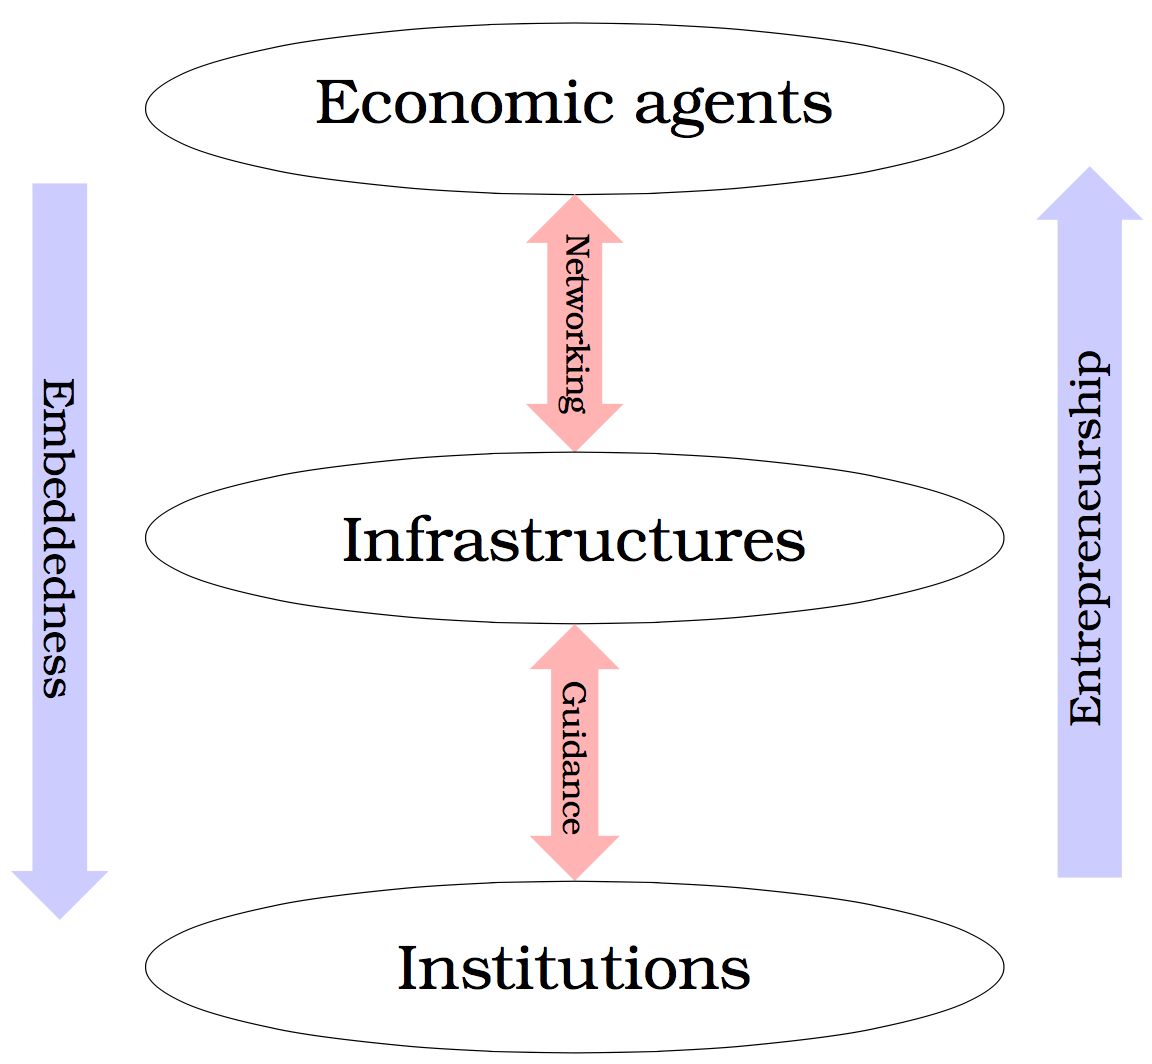
\includegraphics[scale=0.25]{imgs/structure-space.png}
\caption{Schematic representation of the socio-economic space}
\label{spacestructure}
\end{figure}

From Figure~\ref{spacestructure} we note that there exists two polar forces in the socio-economic space. The first is embeddedness; the embedding of the institutional rules into the actions and interactions of individual agents. This force---derived from the institutional structure within the socio-economic space---facilitates the formation of a steady state and adds rigidity to the actions of society. The second is represented in the form of entrepreneurship, which is the force that propagates change in the institutional framework of the economy\footnote{Interaction between economic agents and institutions through entrepreneurship is discussed in more detail in the subsequent chapters. For an excellent discussion regarding the interaction between entrepreneurs and institutions consider \citet{HenreksonSanandaji2011}.}. Society develops through entrepreneurial action and as such entrepreneurship is the antithesis to embeddedness. However, we note that feedback loops---which are a key component of any complex adaptive system---can exist between the actions of economic agents, the interaction infrastructure, and the institutions of society. Entrepreneurship can effect the governance system, which influences the embeddedness of individual agents, and can promote more entrepreneurship.

The schematic representation of the socio-economic space in Figure~\ref{spacestructure} also shows the presence of two other forces: networking and guidance. As has been mentioned above, institutions guide the actions of individual economic agents. As such, the organisational infrastructures that are formed from the actions of agents are directly determined from the institutions within the economy. Institutions guide the actions of individual agents. Networking refers to the resulting networked structure of interaction infrastructures, such that individual economic agents are positioned within a matrix of relations. Agents can arrange themselves within the matrix to positions of power, and again, this can have a feedback loop.

% Our perspective regarding a socially structured governance system is akin to John Commons position on institutional constructs. In addition to collective action of the organised variety, Commons includes disorganised custom, the laws of the state and the common law of the courts, and the patterns of conduct which a community develops for its members. Even when an individual engages in a simple exchange with another, he acts within a framework of collective law and custom, so that collective action has in fact structured the relationship. Social custom and law are perceived to be the product of these interactions. In the process of dealing with each other, bargaining, negotiating, transacting, compromising, they bend and mold their customs, modify the judicial gloss on the law, help to create the very customs which affect their economic relationships. Collective action thus controls the individual; but the individual has some power---especially in concerted effort with others---to modify the nature of collective control \citep{Hodgson2003}.

\subsection{Formalising the socio-economic space and interaction infrastructures}

The socio-economic space is represented in Figure~\ref{spacestructure} as three interacting layers: a population of economic agents; the institutions that the agents accept and trust; and the networked interaction infrastructure---the composition of the social and economic interactions that bind them. These are elements of the socio-economic space that represent the embeddedness of economic agents in a system of governance that encapsulate behavioural rules and exchange mechanisms. The space embraces relationships---consisting of \emph{bilateral economic interactions} and authority chains---or \emph{hierarchies}---formed within the socio-economic space.

\subsubsection{The socio-economic space as a mathematical concept}

A collection of economic interactions on the set of individual economic agents can therefore be regarded as a direct representation of the commonly accepted media and economic institutions that direct the interactions of the economic agents. The interaction infrastructure---including the consumer-producers that form the interactions---are the only visible aspects of the socio-economic space. This perspective of a socio-economic space allows us to make a more rigorous, and therefore more usable, mathematical definition which, by following the embeddedness hypothesis, can be represented as a set of interactions between consumer-producers.
\begin{definition}[Socio-economic space] \label{def:socioeconomicspace}
A \textbf{socio-economic space} refers to a given set of economic agents engaged in a well-described collection of general economic interactions that operate under a well-defined collection of media and institutions. 

For a given collection of media and institutions, a socio-economic space can be represented by a pair ($N, \mathcal{G}$) where $N = \{ 1, \ldots, n \}$ is a given set of economic agents and
\begin{equation}
\mathcal{G} \subset \mathcal{S}(N) \cup \mathcal{H}(N)
\end{equation}
is a given collection of \textbf{general economic interactions} on $N$, where
\begin{equation}
\mathcal{S}(N) = \{ S ~ \mid ~ S \subset N \mbox{ and } S \neq \varnothing \}
\end{equation}
is the family of non-empty coalitions in the population $N$, representing \textbf{lateral} economic interactions on $N$, and
\begin{equation}
\mathcal{H}(N) = \bigcup_{k = 2}^{\infty} N^{k}
\end{equation}
is the class of all finite ordered sequences of economic agents, representing authority chains or \textbf{hierarchical} economic interactions in $N$.
\end{definition}
The collection of all economic interactions, denoted by $\mathcal{G}$, on the set of economic agents $N$ can be regarded as an indirect representation of the commonly accepted media and economic institutions that direct the interactions of the economic agents in $N$. So, $N$ is a mathematical representation of the population and $\mathcal{G}$ is a mathematical representation of the commonly accepted media and economic institutions that guide and determine the interactions between members of the community.

The collection of economic interactions can contain a very large variety of possible economic interactions and forms of interactions. Within our set-up there are two types of economic interactions: \emph{bilateral} economic interactions and \emph{hierarchical} economic interactions. Within this monograph we focus on only one type of economic interaction: the set of simple economic interaction based on equality of the participating economic agents. These general economic interactions $S \in \mathcal{G}$ are denoted as lateral, where $S \subset N$ denotes the pair or group of interacting economic agents.

From the notion of a lateral economic interaction we derive the notion of a bilateral economic relationship. Here, an economic relationship $\{i, j\} \in \mathcal{G}$ is bilateral if the two related parties are equal partners in the generated interaction. Most trade relationships are bilateral as are partnerships in collective decision situations such as production partnerships. Structures of such bilateral relationships form a specific type of structured, collective interaction, called networks.

Although networks of bilateral economic interactions are the focus of our discussion we stress that hierarchical relationships encompass most of our regular interactions within the economy; specifically with regards interaction in a firm\footnote{For a detailed discussion of hierarchies within networked environments consider \citet{Gilles2010}.}. Hierarchical relationships are important for more developed non-primitive socio-economic spaces.

\subsubsection{The structure of interaction infrastructures}

The following definition formalises the main type of economic relationship considered. The collection of economic relationships informs the interaction infrastructure of the socio-economic space, this interaction infrastructure is termed as a network. The definition of networks below encompasses the notion of an interaction infrastructure.
\begin{definition}[Networks] \label{def:networks}
Let the tuple ($N, \mathcal{G}$) be some socio-economic space.
\begin{itemize}
	\item An economic interaction between agents $i$ and $j$, where $i,j \in N$, is \textbf{bilateral} if there is no authority present among the two economic agents constituting this relationship---and as such these two economic agents $i$ and $j$ are `equal' in the generation of the economic values through their relationship. For notational ease this bilateral economic relationship is represented as $ij \in \mathcal{G}$.

	\item A \textbf{network} is a collection of bilateral economic relationships on a given set of economic agents. Thus, a network $g$ based on $\mathcal{G}$ is given by
	    \begin{equation}
	    g \subset \{ ij \in \mathcal{G} ~ \mid ~ i,j \in N \} .
	    \end{equation}

	\item A \textbf{complete network} is a network in which all economic agents are connected to each other by some bilateral economic relationship. Thus, a network $g$ is complete if and only if
	    \begin{equation}
	    g = \left\{ ij ~ \mid ~ i,j \in N \mbox{ and } i \neq j \right\} .
	    \end{equation}
	We denote a complete network on $N$ by $g_{N}$.

	\item An \textbf{empty network} is a network in which there exists no economic interactions between the population of $N$ consumer-producers~\footnote{An empty network is a representation of a monadic economy discussed as given in Definition~\ref{def:autarkyproblem}}. Formally, a network $g$ is empty if and only if $g = \varnothing$.
\end{itemize}
\end{definition}
A network is a derived notion such that the structure is part of the collection $\mathcal{G}$. Models that partition the demand and supply of a trade situation suggests that bilateral interaction between agents are conducted in a bipartite manner such that one side of the interaction is designated as the supply-side and the other side is designated as the demand-side. Models that partition the demand and supply of a trade situation are described in the form of a bipartite network.
\begin{definition}[Bipartite networks] \label{def:bipartiteNetworks}
A network $g$ on a set of economic agents is \textbf{bipartite} if there are two disjoint coalitions $N_{S} \subset N$ and $N_{D} \subset N$ with $N_{S} \cap N_{D} = \varnothing$ such that $ij \in g$ implies that $i \in N_{S}$ and $j \in N_{D}$. Hence, the only feasible economic relations are between a member of $S$ and a member of $D$. Naturally, $S$ and $D$ refer to the supply and demand side in the bipartite network $g$.

\noindent A bipartite network $g$ is \textbf{complete} if $g = N_{S} \otimes N_{D} = \{ ij ~ | ~ i \in N_{S} \mbox{ and } j \in N_{D} \}$.

\noindent A bipartite network $g$ is \textbf{minimally connected} if every consumer-producer in $N$ is engaged exactly one economic interaction each.
\end{definition}
By allowing there to exist a dichotomy between the demand and the supply-side of economic interaction markets of bilateral interactions are represented as a bipartite network. These models partition a set of economic agents into a set of consumers (demand) on one side and a set of producers (supply) who produce some output on the other. Given some set of valuations for the producers output, consumers form trade relationships with suppliers given the actions of all other consumers in the market and the price levels that naturally emerge from the demand and supply for these tradable outputs. These discussions introduce the notions of perfect competition, monopoly, and traders within a bipartite network.

We do not draw such a strict dichotomy between the consumption and production of agents. Instead, as noted in Axiom~\ref{dichotomyhype}, we structure economic agents as both consumers and producers endowed with both consumptive properties and production possibilities. The consequence is a network that can take forms that are potentially divorced from the bipartite structure. Representing economic agents as consumer-producers can naturally lead to the formation of irregular and elongated economic networks. Small-world and scale-free networks can also arise depending on the exchange mechanism imposed. Within these structures individual agents have differentiated positions. These positional attributes can be distributed in an unequal fashion across the network leading to unique opportunities and constraints for agents that possess certain positions in the network.

For completeness we note that another common structure found in both theory and reality is a \emph{star network}, which is referred to in later discussions of network centrality.
\begin{definition}[Star network] \label{def:starNetwork}
A network $g \subset G_{N}$ on $N$ is a \textbf{star} if there exists some consumer-producer $h \in N$ such that
\begin{equation}
g = \left\{ ih ~ \mid ~ i \in N \mbox{ and } i \neq h \right\}.
\end{equation}
Therefore consumer-producer $h$ is at the center of the star.
\end{definition}
This section has provided some structure to the relational theory in two ways. First, we provided an environmental concept that acts to encapsulate the fundamental notions of the relational perspective: this was defined in terms of the socio-economic space. Second, we added structure to the socio-economic space by defining it in mathematical terminology. The insights discussed in this section help in the formal discussion later in the monograph.

The socio-economic space is a dynamic concept. As noted by the schematic representation of the socio-economic space in Figure~\ref{spacestructure} this dynamism is triggered by pressures that derive from entrepreneurial activities. We elaborate on the \emph{states} of the socio-economic space and the mechanism of development through entrepreneurial activity.

\section{States of the socio-economic space}

Particular economic states can be identified through the characteristics of the governance system and interaction infrastructures, which economic agents are ultimately embedded and operate within. At this point we do not comment on how one economic state transitions to another other, but instead focus on potential states that can exist. It is unlikely that the space merely tips from one state to the other; it may indeed be a gradual phase transition of self-reinforcing institutions that are punctuated by institutional and network alternations, which are reflected in notable changes in certain aspects of the governance system.

\subsection{Pure states of the socio-economic space}

A `pure' economic state is one that can only be achieved at a theoretical level. Pure economic states will not exist in reality. Here we provide two pure states of the socio-economic space. The first state---\emph{the state of nature}---describes a relatively primitive socio-economic space whereby institutions and systems of governance exist to obstruct the formation of functional social and economic interactions leading to a difficulty in the generation of wealth throughout the economy. This is not to say that institutions do not exist at all, but the institutions that do exist are either too costly to facilitate exchange or they are formed specifically to hinder the formation of economic relationships between agents. We note that the state of nature can exist as a manufactured state to, for example, suppress an underclass. The second state---\emph{the trustified economy}---refers to a socio-economic space in which corporations have a significant impact on the development of the economy. Specifically the role of competition, the development of new firms, and new the exploitation of new entrepreneurial opportunities are not the driver of change; but pre-existing companies monopolise the development of the governance system. Note that these states should only be considered as theoretical extremes, not a realistic indication of the socio-economic space.

\subsubsection{The state of nature}

In \emph{Leviathan} \citet{Hobbes1651} discusses the emergence of monarchs and governing bodies through the formation of a social contract. According to Hobbes a civilisation could raise itself from a `state of nature' to the formation of functional relationships ultimately governed by absolute government in the form of a monarch. From this structure of rule and enforcement, built on the basis of social contract, civil society could flourish.

The state of nature considered by Hobbes was characterised by the non-existence of, or presence of dysfunctional, social and economic relationships between individual agents. According to Hobbes men are born equally; from this equality, and the inherent violence of man, Hobbes claimed that this would lead to wars and conflict among men so that, ``during the time men live without a common power to keep them all in awe, they are in that condition which is called warre; and such a warre as is of every man against every man''. During this state every person has a liberty to to anything one perceives as necessary for preserving one's own life; and thus life would be, ``solitary, poor, nasty, brutish, and short''. This is the war of all against all whereby cooperation and the presence of functional, wealth-generating social and economic interactions are non-existent.

The essence of this economic state is developed from Thomas Hobbes' initial depiction of the state of nature. However, we do not assume the absence of systems of governance, but instead consider a socio-economic space comprised of dysfunctional systems of governance and therefore the formation of economic interactions between agents is costly. These may be imposed from a top-down manner from an oppressive elite. This results in a \emph{monadic} economy whereby all economic agents act autarkically thus consuming their own output only. Under the state of nature the organisation of society is in its simplest form. In line with Hobbes, the state of nature requires no trust between agents and institutions; and, as such, welfare is at its most primitive.

We do not specifically advocate that this state has ever existed or can exist. The formation of simple institution such as signalling or emotional gesture in which to base simple relationships is also an evolved part of the human species. We are social creatures, and as such, social relations are fundamental and this state of nature is purely theoretical. Alternatively, it can be likely that institutions and systems of governance exist but the costs of using them or even understanding them are too high. In this case the interaction inefficiency is excessive and the formation of social and economic relationships suffer. Given high levels of interaction inefficiency an economic state may revert to a state close to that of the state of nature or monadic economy. As a consequence all economic agents earn near subsistence levels of utility. 

The ultimate claim of this state of nature is that the governance systems are deficient for the society to form structured relations with each other. This deterioration of social and economic capital degrades the structure and development of the governance system. \citet{Granovetter1992} noted that a lack of trust and social capital within society would stifle the creation and development of institutions and organisational patterns of production. In stipulating the construction of institutions \citet[p.~7]{Granovetter1992}, ``economic institutions do not emerge automatically in response to economic needs. Rather,they are constructed by individuals whose action is both facilitated and constrained by the structure and resources available in social networks in which they are embedded.'' He elaborates by providing a discussion of how lesser-developed economies are unable to form recognised firms and elaborate exchange networks. This is also discussed later by \citet{deSoto2001} and \citet{AcemogluRobinson2012}. The state of nature is a more extreme version of the social and economic environment discussed by these authors; the systems of governance are sufficiently dysfunctional such that social and economic relationships are nonexistent, and each agent effectively operates at substance levels.

% This state of the socio-economic space may have equally been attributed to Malthus due to the consequence of the `Malthusian trap'. In \emph{An Essay on the Principle of Population} Thomas Malthus (1798) discusses how without war, disease, or natural disaster the growth rate of the worlds population was exponential whilst the growth of the worlds food-stock was arithmetical. Therefore, according to Malthus' logic, the growing population size would eventually outstrip the food supply leading to the eradication of society as a whole unless `preventative checks' and `positive checks' were applied to regulate the population against the food supply. In Malthus' terms a preventative check was one that was socially developed and would thus lead to a relative stagnation of the population. These preventative checks included abstinence and marriage restrictions. A positive check was a naturally occurring phenomena that would balance the demand and supply of food. Specifically a positive check included starvation and war.

% The state of the world proposed by Malthus leads to the emergence of a so-called Malthusian trap which, according to many economists (Fogel, 2004; Clark, 2007), occurred for much of human history. A Mathusian trap exists when the per capita income within an economy is largely stagnant due to the emergence of new technology leading to population growth as opposed to improvements in the standard of living. Such a phenomenon suggests that over time per capita income does not improve, technology development is slow and largely ineffective, therefore the state of the world is stagnant as economic agents earn subsistence levels of utility; as can be seen in the Hobbesian economy.

\subsubsection{The trustified economy}

The trustified economy is characterised by the centralisation of influential power of the governance system to platforms, or corporations. This power is derived from increased bargaining power with the \emph{de jure} elite due to their economic resources and from their ability to fund research in innovation. Development is monopolised by the power of \emph{de facto} elites.

Whilst witnessing the rise of large corporations largely supported by trusts---such as Standard Oil, J.P. Morgan \& Co. and General Electric---Joseph Schumpeter first discussed the notion of a trustified economy, or more precisely ``trustified'' capitalism as opposed to ``competitive'' capitalism, and hypothesise a trend of economic progress towards this trustified state. Within this trustified state \citet[p.~384]{Schumpeter1928} claimed that, ``[i]nnovation is... not any more embodied \emph{typically} in new firms, but goes on, within the big units now existing, largely independently of individual persons. It meets with much less friction, as failure in any particular case loses its dangers, and tends to be carried out as a matter of course on the advice of specialists. Conscious policy towards demand and taking a long-time view towards investment becomes possible''. Development in the trustified state becomes `automated', increasingly impersonal and decreasingly a matter of leadership and initiative.

The trustified state suggests that the waves of \emph{Creative Destruction} are diluted---or, in an extreme sense, non-existent---compared to competitive capitalism in which new firms enter the economy and displace old obsolete firms. Innovation in competitive capitalism is embodied by entrepreneurs and the foundation of new firms, ``... improvement is forced on the whole branch by the processes of underselling and of withdrawing from them their means of production, workmen and so on shifting to the new firms; all of which not only means a large amount of disturbance as an incident, but is also effective in bringing about the result, and to change `internal' economies into `external' ones, only as far as it means disturbance'' \citet[p.~384]{Schumpeter1928}. This is different in a trustified state of capitalism. Within a trustified state there exists little disruption from entrepreneurs or groups of entrepreneurs through the provision of new firms, new innovative outputs, new production processes, new socio-economic roles, or new political agenda. Instead a paradox arises whereby innovation becomes frequent, predictable and, as a consequence, tedious; doing little to improve society's welfare or even disequilibriate the economy.

Moreover, according to Schumpeter, the trustified state encourages more focus on the automation of processes and, although the division of labour deepens and new socio-economic roles born, the effect is an alienation of individuals and an enlarged separation between the actions of individuals and their overall outputs. This is a typical Marxian conclusion regarding the evolution of capitalism, later repeated by \citet[p.~77]{Milgram1973}: ``....as soon as there was a division of labour things changed. Beyond a certain point, the breaking up of society into people carrying out a narrow and very special jobs takes away from the human quality of work and life. A person does not get to see the whole situation but only a small part of it, and is thus unable to act without come kind of overall direction. He yields to authority but in doing so is alienated from this own actions.'' In fact, Schumpeter's and Marx's ultimate conclusion for the state of capitalism are not dissimilar. In his concluding sentence \citet[p.~386]{Schumpeter1928} hypothesised that, ``[c]apitalism, whilst economically stable, and even gaining in stability, creates, by rationalising the human mind, a mentality and a style of life incompatible with its own fundamental conditions, motives and social institutions, and will be changed, although not by economic necessity and probably even at some sacrifice of economic welfare, into an order of things which it will be merely matter of taste and terminology to call Socialism or not.'' The trustified state was, to Schumpeter, the final stage of capitalism.

The ultimate conclusion of Schumpeter is stark and debatable---a debate that is certainly beyond the scope of this monograph. Instead, our notion of the trustified economy utilises Schumpeter's initial claim regarding the influence of large firms to monopolise innovation, and therefore motivate a change to the governance system and propagate the development or regression of the socio-economic space. With respect to the neoliberal economy less emphasis is placed on individual entrepreneurs and Government to direct development, and more emphasis is placed on pre-existing firms and sources of financial capital. The socio-economic space is therefore characterised by increasingly hierarchical relations within the context of sprawling production organisations.

There are three concluding points to note. First, within the trustified state the action of entrepreneurship is completely replaced by the action of management who exist within transnational firms. Second, is that the trustified economy is only considered as a `theoretical extreme', in that it is unlikely that individual or coalitions of entrepreneurs will become completely redundant and the the supply of new firms to the economy will stop. Furthermore, it is unlikely that the role of government be displaced by corporations and that elected individuals will relinquish their powers to affect the institutions of the governance system. Second, role-building costs and interaction inefficiencies are considered to be reduced due to the presence of more structured institutional environments.

% \subsubsection{The Marxian economy}

% Need discussion on `theoretical communism' here!

\subsection{Representative economic states}

By extending the theoretical extremes of the pure economic states above we provide a typology regarding all more realistic, or \emph{representative}, economic states of the socio-economic space. We specifically provide insight regarding three of these states that have been recorded over time. Each state signifies a notable difference in the governance system and the interaction infrastructures present in the socio-economic space. 

As a socio-economic space develops we tend to see a more structured vertical division of labour and a deeper division of labour with objective socio-economic roles organised by hierarchical relationships. Therefore, in order of development these representative economic states are: (1) the Platonian economy; (2) the incorporated economy; and (3) the Platform economy.

\subsubsection{The Platonian economy}

The Platonian economy is perceived as a `human' or `organic' economy within which the source of wealth emerges through social organisation founded specifically through human ability, specialisation, and limited innovation. It is the ability for humans to organise social production situations within a networked market that is the source of all wealth in this economic state. The organisation of economic activity can only be done on the basis of a controlled and ordered society; specifically ordered through the creation of accepted primitive rules of exchange, well-defined socio-economic roles, and behavioural norms. Thus, governance systems exist to form functional relationships.

Within a Platonian economy agents are assumed to be equal parts when interacting and cooperating with each other. Within predominantly tightly-knit networks relatively small communities tend to favour simplistic conventions of trade, thus facilitating egalitarianism and fairness; no economic agent tends to be more powerful than the rest meaning that hierarchy is primitive. However, positional power may emerge from the socio-economic roles that individuals specialise in.

This type of organisation provides the basis for specialisation and the creation of socio-economic roles completely dependent on an individuals' abilities and on the actions and specialisations of the local society. Within this type of economy, socio-economic roles are primitive, which means that an individuals' specialisation will be purely dependent upon their local socio-economic environment which includes the current organisation and specialisations of those in society, the resource base, and the technology that is apparent within the economy. The resulting coordinated specialisation of an individual results in a higher productivity and wealth creation in society. In other words, the human ability to coordinate allows for the access to increased productivity through specialisation as well as for the realisation of the resulting gains from coordinated social production.

We denote this primitive state of the socio-economic space as the Platonian economy due to the time and context of Plato's writing, which, as mentioned in our discussion of the division of labour in Chapter~\ref{ch:relationalperspective}, focuses primarily on the horizontal division of labour. In his writings of city formation he claims that the majority of economic interactions exist within a market context with a horizontal division of labour. This interaction is outside of the environment of a well-defined organisation such as firms or corporations, and thus a vertical division of labour. During his time of writing corporations did not exist and it is unlikely that firms, even in the most primitive sense of the word, existed to a notable extent. More centralised and organised production techniques are the feature of a more developed socio-economic space. These indeed play a prominent role in incorporated and Platform economic states.

The human species recognised early that individuals, with the ability to specialise in a variety of productive tasks, can be socially organised to achieve a society that generates collective economic wealth. This social organisation is subject to not only increasing returns to specialisation, but when working together, increasing returns to scale. This social organisation is usually called the `social division of labour' and forms the foundation of any human society. The organisation of the Platonian economy refers to the division of specialised tasks among individuals within a human community. It refers to the social organisation of a community to achieve a collective social economy that is collectively subject to increasing returns to scale in its productive abilities. Within a social division of labour individual economic agents assume individualised production tasks. This requires that individuals perform tasks that are recognisable by all members of the society as socially acceptable and economically viable.

This social recognition involves two elements. First, the social recognition of an economic, productive task requires that the task is performed with socially recognised inputs and outputs. Thus, each task within a social division of labour concerns the conversion of socially recognised and specified inputs into socially identifiable and measurable outputs. Second, the social division of labour is only functional as a social organisation if the generated socially recognised outputs can be distributed among the members of the society in a socially recognised fashion. In economic terms, the generated outputs are publicly exchangeable with outputs generated by other specialised individuals. Such a public exchange can only occur through socially recognised exchange mechanisms.

These two elements leads to the conclusion that a social division of labour requires a supportive governance system. As mentioned previously, all economic interaction has to be considered to be embedded in an appropriate social governance system. The embeddedness of economic interaction within a governance system is fundamental to our understanding of the organic Platonian social economy. We can loop this back onto the interpretation and clarification of the social division of labour as a system in which individual production tasks are combined with economic exchange. Indeed, the organisation of social economy is formed as a social division of labour in which individuals execute specialised productive tasks and exchange the resulting outputs from these tasks through socially recognised exchange mechanisms.

The nature of the horizontal and vertical social division of labour is that tasks are performed in a structured sequence. This allows the production of relatively complex consumption goods: such goods are realised through a sequence of intermediate stages performed by distinct specialised individuals. The Platonian economy allows for this and this form of exchange through intermediaries is used throughout Chapters~\ref{ch:criticalnodes} and~\ref{ch:blocks}. Under this structured sequence of exchange economic agents can fully utilise their relational attributes.

Platonian economic states can be characterised by high role-bulding costs. Within primitive environments agents engage in a process of adaptive specialisation due to the absence---or relative deficiency---of more structured educational institutions. In more advanced Platonian economies roles can be built through apprentice and kinship relations, therefore agents will dictate the specialisation of individual economic agents. Moreover, patrilineality and family ties can also play a distinct role. We note the importance of these institutions to support role-building and specialisation with respect to the case of Renaissance Florence in Chapter~\ref{ch:entrepreneurship}. \citet{NorthWallis2006} suggest that in primitive societies the identities of individual agents were based prominently on social roles as opposed to the economic context of their roles. As such, the identity of individuals was based more on the characteristics and patrilineal ties of the individual as opposed to the economic position and ties of the individuals. Specifically, the reputation and perhaps the role of the individual would have depended more on the family of the individual as opposed to the socio-economic role that the individual autonomously specialises into. As our society has developed, and we require interacting with a greater wealth of individuals, more emphasis has been placed on the importance of socio-economic roles and related action-sets as opposed to more personal identities.

We conclude that the social division of labour results into well-structured social production chains, naturally resulting into the conclusion that the economy is founded on a complex network structure. These complex networks are initially shown in the Platonian economy. Again, we generalise this insight beyond the constrained view of the social division of labour and apply this to any human economic interaction.

\subsubsection{The incorporated economy}

A socio-economic space can include hierarchical relations as well as purely economic exchange relations. We contend that as the socio-economic space develops the economic interactions and relationships that emerge within it become progressively hierarchical and the governance system, including the socio-economic roles, become more structured. The Platonian economy omits the existence of `hierarchical production organisations'. These organisations---generally regarded as firms or corporations---internalise relationships between specialised individuals through an authority guidance structure. This organisational form clearly delineates incentives and makes the guidance of decisions and tasks more transparent and effective than through the more organic horizontal division of labour. Instead of individuals being guided by external forces, they are subordinated within an authority structure. The result is the existence and fruition of a vertical division of labour based on some incomplete labour contract.

The introduction of hierarchical production organisation requires the development of a more structured governance system, typically through entrepreneurial effort, and can lead to the generation of a deeper division of labour with more automated socio-economic roles. The horizontal division of labour in the Platonian economy suggests that all economic exchange is conducted within a network by a set of equal socio-economic agents in terms of their authority. Typical interaction inefficiencies exist with regards the existence of transaction costs \'{a} la \citet{Coase1937} and \citet{Williamson1971, Williamson1975, Williamson1979}. From this perspective we can see that as interaction inefficiencies increase in the exchange networks a horizontal division of labour is substituted for a vertical division of labour and the exchange networks are shortened accordingly.

The incorporated economy illustrates the benefits of increasing returns to specialisation from the automatisation and deepening of the division of labour within a coordinated and centralised environment. Hierarchical production organisations within this state are considered to be the workhorse regarding the generation of wealth throughout the socio-economic space. Therefore, organisation within an incorporated economy deviates from a Platonian economy in this regard. Specifically, within an incorporated economy the economic decision-making by individual agents is more centralised within a hierarchical structure, and therefore the majority of strategic decision-making is done by `principals' and subsequently carried out by `agents'. Relationships within a firm are incomplete in the sense that the principle usually has insufficient ability and information to precisely assess the task and performance of the agent. This is due to the specialised nature of the tasks done by these individuals within the authority structure. As such, traditional principal-agent relationships based on information asymmetries arise as the majority of economic agents suffer from a loss of autonomy \citep{JensenMeckling1976, Eisenhardt1989}.

The consequence of the formation of hierarchical production organisations is that decision-making is more interdependent and the interactions that exist between agents are embedded within a well-defined, structured and accepted governance system. Moreover, socio-economic roles become more structured and automated, which facilitates the invention of technologies to substitute and complement existing divisions of labour. The incorporated economy is the first economic state in which the social division of labour---which is the only form of the division of labour in the Platonian economy---is rivalled with a division of labour within the firm as explicitly discussed by Adam Smith. Thus, the incorporated economy is the first state to introduce both bilateral and hierarchical economic interaction: the Platonian economy was restricted the assessment of bilateral economic interaction only. Standard transaction cost and contract theory \citep{Cheung1983, AghionHolden2011} regarding the establishment of the firm against economic interaction within a market environment apply here.

As noted by Coase, inefficiencies naturally exist within both firm and market interactions; however, the establishment of firms aims to minimise these. This suggests that the interaction inefficiency of an incorporated economy is high, but lower than the inefficiency within a Platonian economy. The institutions are relatively well-defined, but are still costly to use. These costs depend on how well defined they are, and how available more formal institution are to society as a whole. The government has some role to play in the maintenance of these institutional structures.

\subsubsection{The Platform economy}

A Platform economy is one that is most closely related to that of a contemporary developed economy. Under this setting the notion of a hierarchical production organisation is further developed from the incorporated perspective---considered as firms and corporations---through the formation of elongated hierarchical relationships and the increasing returns from a deepened division of labour, economies of scale, and economies of scope. Developed hierarchical production organisations have more prominence and power in a Platform economy than in an incorporated economy; however their structure and scope is larger. As opposed to witnessing hierarchical economic interaction within the context of a firm or corporation we now see this interaction within vaster and more complex structures that we term as a \emph{platform}.
\begin{definition}[Platform] \label{def:platform}
An economic agent or hierarchical production organisation is a \textbf{platform} if it exists in multiple aspects of a socio-economic space and facilitates interaction between aspects between these for other economic agents and hierarchical production organisations.
\end{definition}
A platform is an economic agent or hierarchical production organisation that, due to its position and multivocality, has an ability to enable economic interaction between aspects and can potentially extract from other economic agents by brokering relations. Thus, a platform can both \emph{enable} the formation of economic interactions and can \emph{extract} the wealth generated from these interactions. As a consequence, a platform is a hierarchical production organisation that operates within different aspects of a socio-economic space and as such is able to monopolise interaction both between and potentially within those aspects. We could consider a platform as a middleman that operates in many aspects of a socio-economic space---combining multiple socio-economic roles---and as such monopolises exchange between those those aspects.

In conventional syntax we may associate a platform with an uncontested transnational corporation or conglomerate which, by virtue of their function and place in the economy, operates in multiple sectors and has an ability to connect those sectors together. This may be done through the facilitation of economic interactions between those sectors---much like a `market-maker'---or alternatively done by producing an intermediary output that has function within multiple sectors. The defining feature is that platforms have power in multiple sectors of an economy and can use that to their advantage.

The deepening of the division of labour and the subsequent automatisation of roles, first introduced in the incorporated economy, is recorded to a greater extent within platforms. Production processes carried out by technology leads to considerable depersonalisation and redundancy of the `human' division of labour. The consequence is two-fold: first, the redistribution of the population to more productive socio-economic roles; and second, is a redistribution of wealth to those more productive roles. Thus, any friction in terms of role-building costs may lead to an unequal distribution of wealth and utility within society.

\medskip\noindent The assessment of economic states implies that the socio-economic space is a dynamic concept that develops over time. Moreover, an inference from the assessment of different socio-economic states is that the development of the socio-economic space---the context of the roles and interactions, the institutional structures, and the elements of the governance system---brings with it a progressively hierarchical society. More complex structures arise and are built upon as the space of interactions evolves from a monadic state of nature, to a primitive Platonian economy with general economic interactions, to an industrialised incorporated economy with hierarchical production organisations, to a Platform economy, and finally to a trustified economy. 

The evolution of the socio-economic space also illustrates tendency toward a wider array of well-defined socio-economic roles, a more distinctive presence of automated `non-human' or `inorganic' socio-economic roles, and more sophisticated institutionalised structures for supporting a deepened division of labour. The driving force of this development is the actions of entrepreneurship. Below we introduce the notion of entrepreneurship within the context of growth and development of the socio-economic space.

\section{Growth, development, and the entrepreneur}
\label{subsec:growthdev}

Figure~\ref{spacestructure} introduces a set of important forces within the socio-economic space. We have already discussed the forces of embeddedness with respect to socio-economic roles, networking with respect to formation and structure of interaction infrastructures, and guidance with respect to institutions within the governance system the guide interaction and behaviours. Our discussion thus far has, however, been deficient with respect to the force of entrepreneurship, which acts to influence a change within the layers of the socio-economic space. The act of entrepreneurship is closely related to the development of the socio-economic space, and its transition from one state to another. Importantly, it is an action that impacts all three layers of the socio-economic space: the population of economic agents, the structure of the interaction networks, and the institutions within the socio-economic space.

\subsection{Distinguishing growth and development}

The growth and development of the socio-economic space are considered as two distinct but related processes. Both lead to similar outcomes---the improvement or redistribution of aggregate utility across the population of economic agents---however, the distinction between them is important; particularly for the discussion of the entrepreneur and entrepreneurship. Their distinction can be highlighted in the set of definitions below.
\begin{definition}[Growth and development] \label{def:growthanddevelopment}
A socio-economic space can grow and develop. These are two distinct notions.
\begin{itemize}
	\item The \textbf{growth} of a socio-economic space refers to a change in some fundamental or pre-existing parameters that define the socio-economic space such that the aggregate utility of all economic agents increases.

	\item The \textbf{development} of a socio-economic space refers to a productive change in the elements of the governance system such that the new institutional mechanisms produces an increase in aggregate utility.
\end{itemize}
\end{definition}
The growth of a socio-economic space corresponds to changes in parameters that describe the economic agents, the extent of their actions and specialisation, and the size of the space they interact in. These parameters include the size of the population of economic agents, the cost of interaction and the size of the interaction inefficiency, and the extent of their individual production technologies. Improving changes in these parameters leads to an increase in aggregate utility, however the structure of the interaction infrastructure and the exchange conventions remain constant. Importantly, the composition of the governance system remains constant given the growth of the socio-economic space.

The development of a socio-economic space corresponds to a direct alteration in the composition of the governance system. These alterations include the creation of a new socio-economic role, socially recognisable output, trading mechanism, or interaction infrastructure. Improving changes can lead to the extension of the division of labour or organisation of society given the rule sets provided by the institutional framework.

Despite differences in definition, the notions of growth and development are related such that the development of the socio-economic space through, say, the deepening of the division of labour can lead to the growth of the socio-economic space through the improvement of production technologies or the facilitation of previously unconnected economic agents to exchange with one another. In this way the notions of growth and development interact with one another: a socio-economic space can go through a relatively slow process of growth and then a period of development which prompts a punctuated change in the equilibrium organisation of society; this itself induces a period of growth.

% % % Can be brought to the Appendix

\subsubsection{Decline, regression, and The Edge of Chaos}

Equally as interesting are the notions contrary to the growth and development of the socio-economic space: namely \emph{decline} and \emph{regression}. The decline of a socio-economic space---as considered the opposite of growth---refers to a change in some fundamental parameters that induce a decline of aggregate utility of all economic agents. An example of this decline can be a reduction of an economy's population leading to a reduction in its Gross Domestic Product\footnote{The fall in Japan's Gross Domestic Product since 2010 can be illustrative of the decline of a socio-economic space in the form of a population decline \citep{Economist2014}. However, some see it as a consequence of more fundamental Japanese cultural norms backed by formal institution \citep{West2011}.} or can be a reduction of productivity due to a deterioration of an economy's capital base. Again, the decline of a socio-economic space, much like its growth, is typically classified as a relatively slow process.

On the other hand, the regression of a socio-economic space---as considered the opposite of development---refers to a destructive alteration of the governance system which induces a fall in aggregate utility across the population of economic agents. Examples of this include the adoption of a behavioural or cultural norm that reduces productivity, the deterioration of educational institutions, or the presence of ill-defined or perverse institutions that do not facilitate functional wealth-generating economic interactions\footnote{An appropriate example is the recent global financial crisis and subsequent sovereign debt crisis. Many see this crisis as a symptom of an institutional malaise \citep{Crotty2009, Ferguson2014} as well as a fundamental outcome of the economics discipline itself \citep{Hodgson2008, Hodgson2009, Krugman2009}.}. Much in the same way as development, the regression of a socio-economic space can be a punctuated event.

The theory of punctuated equilibrium is extremely important. The economy as a complex adaptive system can gravitate towards a so-called `Edge of Chaos' : the fertile ground between too much order and too much randomness; a concept attributed to Christopher \citet{Langton1990}, and subsequently popularised in finance literature by Nassim \citet{Taleb2007, Taleb2013}. Self-organising systems of interdependent parts progressively optimise to a certain point whereby any deviation will cause the system to malfunction and collapse. This edge of chaos terminology can be used to describe the institutional structure and the resulting dynamics of economies. In the final chapter of \emph{Civilisation}, Niall \citet{Ferguson2011} argues that empires---the Roman, the British, the French---experienced a punctuated collapse. This is an argument also discussed by Jared \citet{Diamond2011}. In their evolutionary strive for efficiency they develop networks and institutions that are highly interdependent, meaning that if one network or institution were to collapse the economy as a whole could tip into failure. In the strive for efficiency a socio-economic space can become highly prone to failure. Such an observation fits well with the potential unraveling of interdependent forms of trust.

% % % 

\subsection{Entrepreneurship and the entrepreneurial function}
\label{sec:entrepreneurship}

The development of the socio-economic space is propagated by the actions of the \emph{entrepreneur}. It is the entrepreneur---through the process of \emph{entrepreneurship}---that facilitates the evolution of the socio-economic space through the modification of the elements of the governance system and, as a consequence, alters the welfare of economic agents that use the governance system to interact. 

The entrepreneur is essential in the transition and maintenance of a certain type of economy, and whose function gathers importance as the socio-economic space develops. For example, in the state of nature entrepreneurship and the entrepreneurial function is absent due to the dysfunctional governance system and the non-existence of social and economic relationships. On the other hand, in a trustified economy entrepreneurship is common and routinised by non-personal economic agents. In the trustified economy changes to the governance system are regular and subject to change from one time period to the next. The development of entrepreneurial models built with the intention of encompassing institutional and social aspects are of paramount importance as their ultimate role will indeed depend on the structure of the socio-economic environment which they operate in \citep{AldrichMartinez2007}.

The schematic in Figure~\ref{spacestructure} notes that the socio-economic space can be partitioned into three distinct layers, namely: the population of economic agents that interact within the socio-economic space; the infrastructures that are created from their interaction; and the institutions that reflect and enforce the rules of interaction. We note that the act of entrepreneurship operates in all layers of the socio-economic space described. Entrepreneurship can, for example, lead to the provision of new products and processes that increase the production sets of a population of economic agents, provide a new architecture to existing interaction infrastructures, or lead to the modification or introduction of new institutional structures. We provide definition to these concepts below.

\subsubsection{Defining entrepreneurship and the entrepreneurial function}
\label{definingentrepreneurship}

An entrepreneur refers to an economic agent that engages in entrepreneurship, a set of actions that refer to a higher form of adaptive specialisation within a given socio-economic space.  Entrepreneurship is an action or set of actions taken by individual economic agents that go beyond the choice space defined and imposed through the prevailing governance system of the economy. This specialisation affects two categories of the socio-economic space: the governance system itself, and its networked interaction infrastructure. All actions that result into new developments in the governance structure or in the trade infrastructure underlying the economy can be regarded as ``subjective innovation'', since these entrepreneurial actions---and subsequent innovations---usually derive from actions already exhibited by individuals within a given socio-economic space.

The \emph{entrepreneurial function} is a weaker notion than that of entrepreneurship and should be considered separately. Both are considered as actions that impact the socio-economic space in some way, but the most notable difference between entrepreneurship and the entrepreneurial function is that the latter is not necessarily carried out by entrepreneur and as such affects the structure of the socio-economic space in a more minor way. Indeed, the entrepreneurial function, as distinct from entrepreneurship, is the slight modification of a given socio-economic role for operation in a given context or the formation of new economic interactions and relationships with a given socio-economic role and recognisable output. The entrepreneurial function can, and is, conducted by all economic agents of a given population. It does not directly lead to the deepening of the division of labour, the formation of new socio-economic roles, new outputs and technologies, a reformation of the socio-economic space, or new influential positions in the network, and thus does not spur development of the socio-economic space. However, the economic agent can spur growth through the process of the entrepreneurial function.

This discussion of the entrepreneur and the entrepreneurial function allows us to make a definition on which to expand upon throughout the monograph.
\begin{definition}[Entrepreneurship and the entrepreneurial function] \label{def:entrepreneur}
Consider a socio-economic space with a population of economic agents and a governance system of socio-economic institutions.
\begin{itemize}
\item An \textbf{entrepreneur} is an economic agent who, through her actions, engages in entrepreneurship.
\item \textbf{Entrepreneurship} refers to actions that modify in a major way elements of the governance system and the underlying interaction infrastructure in the socio-economic space, thus directly or indirectly impacting the population of the socio-economic space.
\item The \textbf{entrepreneurial function} refers to actions that modify in a minor way elements of the socio-economic space, thus directly impacting the individual economic agent and her local environment.
\end{itemize}
\end{definition}
For clarity we note two main differences between entrepreneurship and the entrepreneurial function from the definition above. These two differences can be distinguished as `scale' and `creativity'. With regards scale we note that entrepreneurship is conducted at a larger scale than the entrepreneurial function. Indeed, the impact of entrepreneurship leads to a change in the structure of the governance system that is used by all agents within the socio-economic space; therefore the process of entrepreneurship directly impacts all agents of the socio-economic space. This is not the case with regards the entrepreneurial function. The entrepreneurial function directly impacts the economic agent conducting it and her connections only. Indeed, it may impact others in the population indirectly, but the effects of the entrepreneurial function are directed and do not lead to a change in the elements of the governance system.

With regards creativity we note that entrepreneurship is inherently innovative and, as such, all subsequent changes to the governance system are new. The creativity of the entrepreneurial function is reflected in the formation of new socio-economic roles, new outputs, new mechanisms of exchange, and new interaction architectures, that are subsequently embedded in the socio-economic space. The creativity of the entrepreneurial function is limited, and thus does not generate anything inherently new in the economy. This distinction with regards the innovativeness of the entrepreneur is important when making a general distinction between the two actions.

Whereas entrepreneurship is the main workhorse for the development of the socio-economic space, the entrepreneurial function along with external parameters such as population growth are the main forces of the growth of the socio-economic space. The evolutionary nature of development and the entrepreneurial function characterised by punctuated changes in the socio-economic space. This notion is based on an initial discussion by \citet{GillesLazarovaRuys2006} who propose the formation of a stable socio-economic space based on a social division of labour of objective socio-economic roles as initially emerging from a state of chaos.

This definition of entrepreneurship is strong relative to the existing literature. Within the relational perspective, entrepreneurship refers to more than self-employment---as is the typical indicator for many analyses of the topic \citep{EvansJovanovic1989, Lazear2004, CagettiNardi2009, SanandajiLeeson2013}---but must include actions that alter the governance system of the economy in a substantial way. As a consequence the notion of entrepreneurship coincides with Schumpeter's perception of the entrepreneur providing a disequilibrating force to the economy. Our point of departure is to claim that the entrepreneur should not be perceived as simply an agent that interacts within a market context; but can actively disequilibrate a socio-economic space through influencing a change to the governance system. Further still, and perhaps most importantly, we accept that entrepreneurship leads to the extension of the division of labour and the development of new socio-economic roles. As a consequence new positions emerge in the socio-economic space and entrepreneurial individuals can build on those positions and potentially earn rents and profits from doing so\footnote{A more elaborate discussion of the socio-economic space is left until the subsequent chapters. The next chapter provides an overview regarding the established theories entrepreneurship and how the relational fits with these established theories.}.

\subsubsection{Entrepreneurship and economic regression}

There exists no reason to suggest that the outcome of entrepreneurship is always positive development. William \citet{Baumol1990}, building on the work of Joseph \citet{Schumpeter1942}, noted that the entrepreneur and entrepreneurship were not always forces for good. Indeed, Baumol claimed that the impact of entrepreneurship depended on the institutional environment of the entrepreneur and, as a consequence, the affect of entrepreneurship could be productive, unproductive, or destructive. If productive, then the impact of entrepreneurship would lead to some increasing welfare for society; if destructive, then the impact of entrepreneurship would lead to decreasing welfare for society; and if unproductive, then the impact of entrepreneurship would have no welfare impact for society.

Baumol's hypothesis can be utilised for our analysis. Indeed, to this point we have aligned our perception of the entrepreneur and entrepreneurship with a productive outcome, i.e., the development and the improvement of society's welfare. However, the perspective of entrepreneurship could equally be applied to the reduction of society's welfare. A number of examples can be noted whereby the welfare of society may be reduced as a consequence of entrepreneurial actions: the full exploitation of a new role and new position within a society; the formation of an uncompetitive structure containing multiple economic agents; the establishment of barriers to entry thus restricting competition; and the control of many competing firms through directorate control.

It is the potential regression of society through the actions of entrepreneurship that are of interest to many economists. Indeed, this relationship between regression and entrepreneurship are discussed in more detail throughout the monograph. In particular we align the network notion of a middleman to that of an entrepreneur whereby the actions of the entrepreneur is to extract value and broker relations and interactions between agents.

\section{Simulating growth and development}

This chapter has provided an elaborate discussion on the definition, structure, growth, and development of the socio-economic space. This final section combines these concepts, and other concepts introduced previously, to simulate the growth and development of the socio-economic space. During this simulation we do not consider the characteristics of the entrepreneur directly, but instead consider the effects of entrepreneurship and subsequent development through changing institutional structures. Growth is simulated with the use of a growing population of economic agents, the emergence of a more sprawling interaction infrastructures, and variability in the production possibilities of the economic agents. We find common interaction infrastructure topologies that emerge with a given governance system and analyse how the distribution of utility is impacted with different institutions.

We analyse a total of eight simulations over two different institutional exchange mechanisms that demonstrate the growth and development of a socio-economic space. Each simulation differs in a number of factors, such as: 
\begin{itemize}
\item[(1)] the production abilities of the economic agents in the outputs considered; and 
\item[(2)] the exchange mechanisms considered that characterise the socio-economic space. 
\end{itemize}
We set up the simulations with an initial discussion on the mechanism of adaptive specialisation, which facilitates the growth of the socio-economic space, and the exchange mechanisms used.

\subsection{Adaptive specialisation and the process of growth}

Throughout our simulations we assume the existence of a given set of well-defined socio-economic roles. Further, we assume that economic agents specialise in an adaptive, as opposed to an objective, manner. Adaptive specialisation requires economic agents to specialise in a costly rationalised way to a socio-economic role such that they actively attempt to maximise their aggregate utility with respect to their local socio-economic environment. Specifically, individual economic agents produce an output bundle and form economic interactions with others subject to the existing elements of the governance system and the outputs, or specialisations, of all other consumer-producers within the socio-economic space. An individual consumer-producer entering a socio-economic space faces a preexisting set of optimising consumer-producers, an exchange mechanism, an interaction infrastructure, and an allocation of tradable economic commodities across those consumer-producers. Given this, an agent optimises her utility over her potential consumption and production plans and the set of the feasible economic interactions with the goal to maximise her utility. The agent must select a production plan and a subsequent set of trading partners that maximises her utility. This optimisation problem is denoted as the \emph{adaptive specialisation problem}, which is discussed further below.

A prerequisite for adaptive specialisation is that there must exist a socially recognised and accepted exchange mechanism such that completed bilateral interactions can emerge as the outcome of the interaction of these exchange mechanisms. These exchange mechanisms are institutions that are common knowledge and act to guide interacting agents to an allocation on the core of the bilateral exchange. In imperfectly competitive environments the institution acts to resolve the indeterminacy of contract proposed by \citet{Edgeworth1881}. Indeed, institutions are required to resolve this problem of trade; they diminish the uncertainty in the formation of the economic interaction thus allowing individual economic agents to calculate with certainty the payoff of forming relationships. Furthermore individual economic agents can choose to specialise in a certain output given the certainty that the institution provides. In this way institutions provide the relative payoffs of society and coordinate specialisation and exchange.

The process of adaptive specialisation highlights a fundamental claim made by institutional economists: that institutions ultimately act as an invisible hand that guides the specialisations of individual agents. The process of adaptive specialisation also highlights the requirement of institutions to form socio-economic roles and facilitate exchange; indeed, the embeddedness hypothesis and the theoretical construct of economic interaction shown in Figure~\ref{fig:governance}. Furthermore, we show that this process also highlights the relationship that the social contract dictated by the governance system can have a direct influence on the organisation of society through the topology of the interaction infrastructure.

\subsubsection{Adaptive specialisation problem}

Adaptive specialisation occurs when an economic agent enters the socio-economic space. When some consumer-producer enters the socio-economic space they can form a number of economic relations, or alternatively operate in an autarkic state if the costs of the interaction---the interaction inefficiency---are too high, or if there are no suitable economic agents to form an economic interaction with. Each consumer-producer aims to select a set of trading partners, a sequence in which to trade with them, and a consumption plan and production plan such that the consumer-producer maximises her aggregate utility across all of these interactions. Further still all interactions must be mutually beneficial such that all simple economic interactions must benefit both agents in the interaction. 

Given a population of consumer-producers, denoted by the set $N$, we denote an economic interaction between agents $i,j \in N$, where $i \neq j$, as an $ij$\emph{-exchange}. The adaptive specialisation problem for some consumer-producer is structured as a five-stage maximisation process. 

\begin{itemize}
	\item[(1)] Some production plan is selected. The output generated from this production plan is used for forming economic relationships. 

	\item[(2)] The consumer-producer uses the output to engage an $ij$-exchange that is both mutually beneficial and provides $i$ with the highest utility. The resulting consumption bundle from the initial trade is used for subsequent $ij$-exchanges. 

	\item[(3)] The consumer-producer reiterates stage 2 with the new resulting consumption bundle in each iteration until all mutually beneficial exchanges are exhausted. The utility is aggregated across all $ij$-exchanges. 

	\item[(4)] The consumer-producer reiterates stages 1 to 3 for all production plans that lie on the convex hull of the production set.

	\item[(5)] The consumer-producer compares overall utilities for all production plans and selects the production plan that provides the highest overall utility.
\end{itemize}

To maximise her utility with respect to her local socio-economic environment a consumer-producer must take into consideration the existing governance system, all potential economic relationships, and the sequence of those relationships that are available to her. The adaptive specialisation problem is given as the maximisation of an agents utility subject to the socio-economic space of specialised agents and systems of governance. For a general way to describe the exchange mechanisms of the governance system the adaptive specialisation problem is given by the following definition.

\begin{definition} \label{def:adaptiveSpecialisationProblem}
Consider a consumer-producer $i = (u_{i}, \mathcal{P}_i)$ and an exchange mechanism given by the governance system $\Lambda$. Consumer-producer $i$ adaptively specialises when she solves the following optimisation
\begin{equation}
	\max u_{i}(x) \mbox{ subject to } x_{j} \mbox{ for all } j \in N \mbox{ and } \Lambda ~ ,
\end{equation}
where $\Lambda$ is the given governance system. The decision problem formulated is known as the \textbf{adaptive specialisation problem}.
\end{definition}

Throughout we assume that the process of adaptive specialisation is myopic; that a consumer-producer is unaware as to whether other economic agents are to enter the socio-economic space and, as a consequence, the economic agent does not consider the potential for other economic agents to enter the space. A consumer-producer only optimises subject to her current environment. We assume that economic agents are unable to forecast the total number of new economic agents that enter the socio-economic space and the utility functions of those agents. An extension may consider a more rational form of adaptive specialisation where a new consumer-producer can anticipate the number of other economic agents that will enter the socio-economic space.

Thus, even though the specialisation of each agent is \emph{ex ante} optimal, such that each agent rationally selects a production plan and trade relationship that maximises their utility, but may not be optimal \emph{ex post}. Due to the fixed nature of the network and the trade relationships the entire network may not be Pareto optimal as new consumer-producers enter the socio-economic space. The decision-making does not consider the further growth of the socio-economic space, meaning that the production plan and trade relationship made by an agent may be \emph{ex post} suboptimal as new agents enter the socio-economic space.

We justify this form of boundedness in three ways. First, it is difficult for economic agents to accurately predict the number of new agents that will enter the socio-economic space indefinitely. Second, it is difficult for agents to know exactly the utility functions of all new agents that are to enter the socio-economic space. Finally, it is difficult for agents to know exactly the production sets of all new economic agents that enter the socio-economic space.

\subsubsection{The process of growth}

The socio-economic space grows through an increasing population and the process of adaptive specialisation. Definition~\ref{def:adaptiveSpecialisationProblem} noted that the adaptive specialisation of a consumer-producer depends on the context of the governance system---in this case indicated by the exchange mechanisms---that the agent uses to form economic interactions. Therefore, due to the sensitivity of the adaptive specialisation process and ultimate equilibrium to the exchange mechanisms embedded within the governance system, we only discuss the basic process of growth before providing a more in-depth discussion with respect to each exchange mechanism below.

The basic process of growth through adaptive specialisation is as follows. Initially, the socio-economic space consists of a pair of consumer-producers who form an economic interaction. Since $\ell = 2$ each consumer-producer will specialise in the production of a single output whereby one specialises in production of $X$ and one specialises in the production of $Y$. A new consumer-producer is added to the socio-economic space and maximises her utility by solving her adaptive specialisation problem in which she selects a production plan from her production set and uses it to trade with a set of other economic agents under the given exchange mechanism.

Economic interaction is based on consent and must be mutually beneficial such that the cost of engaging in the relationship be less than the benefit of the relationship for both consumer-producers.

\begin{definition}[Mutual benefit]
Let there exist some interaction infrastructure given by the set $g \subset \mathcal{G}$ on a set of consumer-producers, $N$, such that $i,j \in N$ and $ij \notin g$. Let $w_{i}, w_{j} \in \mathcal{C}$ be the sets of tradable quantities for consumer-producers $i$ and $j$ respectively.
\begin{itemize}
\item[(a)] An economic interaction between agents $i$ and $j$ is \textbf{mutually beneficial} if
\begin{equation}
u_{i}(g \cup ij) \geqslant u_{i}(g) \mbox{ and } u_{i}(g \cup ij) \geqslant u_{i}(g) ,
\end{equation}
where $g \cup ij$ refers to the resulting network where an economic relationship between $i$ and $j$ has been formed and $u_{i}(g)$ is agent $i$'s utility in the network $g$. This implies that the economic interaction between $i$ and $j$ are individually rational~\footnote{The notion of mutual beneficial interaction also coincides well with the equilibrium notion of \emph{Pairwise Stability}, a fundamental concept for \emph{consent} in social and economic relationships.}.

\item[(b)] The set of $i$'s \textbf{mutually beneficial interactions}, given the network $g$ and $i$'s current tradable quantity $x_{i} \in \mathcal{C}$, is denoted by
\begin{equation}
\mathcal{M}(g,x_{i}) = \left\{ j \in N \setminus i ~ | ~ u_{i}(g \cup ij) \geqslant u_{i}(g) \mbox{ and } u_{i}(g \cup ij) \geqslant u_{i}(g) \right\}.
\end{equation}
\end{itemize}
\end{definition}

Adaptive specialisation requires that the agent initially produces an output that maximises their cumulative utility across all mutually beneficial economic interactions. In this set-up the agent produces an output once and uses this to form an economic interaction with another agent, and so on until there exists no more mutually beneficial exchanges. The economic agent therefore maximises her utility by selecting a production plan that provides her the maximal utility, which is the culmination of all possible economic interactions. At the end of the interaction period all mutually beneficial interactions for each agent are exhausted. The process continues until all consumer-producers have entered the socio-economic space.

This adaptive specialisation process differs from the simple adaptive specialisation process initially considered. Instead of adapting to the socio-economic role of a single agent, an agent interacting within a socio-economic space needs to create an output that they will trade in a sequential manner with a set of other economic agents given a certain exchange mechanism. The process solves the adaptive specialisation problem of maximising a consumer-producers utility subject to the tradable economic goods endowed on the population of economic agents and the exchange mechanisms within society.

We provide simulations regarding the evolution of a socio-economic space under two types of exchange mechanism. In the first case we assume that the existence of an egalitarian exchange mechanism. In the second case we assume the existence of a Cournot-Nash exchange mechanism based on well-defined demand and supply functions. In both cases we assume instances of costless economic interaction---where there exists no interaction inefficiency---and instances of costly economic interaction---where there is some positive interaction inefficiency\footnote{For more information regarding the codes used to simulate these models please consider Appendix at the end of the chapter.}. Further, we compare the architecture of interaction infrastructures that emerge under both institutional trading structures and the resulting utility levels for society. Within this context the movement of a society from one exchange mechanism to another is regarded as an outcome of entrepreneurial activity.

\subsection{Reviewing exchange mechanisms}

For economic agents to specialise, in either an adaptive or objective way, there must exist well-defined institutional structures that facilitate exchange and the formation of relationships. We characterise the institutional structure of the socio-economic space by a set of exchange mechanisms that guide exchange between economic agents. The exchange mechanisms discussed below differ substantially on the complexity of their use and therefore the assumed rationality that we give to the economic agents. The first trade mechanism, egalitarian exchange, is relatively simple and is typically associated with a relatively primitive economic state (Graeber, 2011) and requires low levels of rationality. The second trade mechanism, Cournot-Nash exchange, is more complex and is typical of more developed economic states.

\subsubsection{Egalitarian exchange mechanism}

The first set of simulations establish a socio-economic space based on egalitarian exchange. Egalitarian exchange regards the equal split of the production of all agents engaged in the trade. This is a trade mechanism based on the fundamental idea of equality among all agents within the trade, which---as well as the adherence of fairness---is based on a well-accepted behavioural norm across all economies. This trade mechanism is the least costly and therefore simplifies the trade decisions and the formation of economic relationships significantly. Moreover, we are unable to separate the production and consumption decisions: the resulting consumption decision is primarily based on the production decisions of each economic agent.

Consider an economic relationship between a set of $N$ consumer-producers where $|N| = n$. There exists $\ell$ economic goods within the socio-economic space and each agent $i \in N$ has a bundle of goods $x_i \in \mathbb{R}^{\ell}_{+}$. The egalitarian exchange mechanism can be described by the notion that all output bundles are collected and divided equally among all $n$ agents. Each consumer-producer $i$ will receive the same bundle, given by
\begin{equation}
E(x) = \frac{1}{n} \sum_{i \in N} x_i \in \mathbb{R}^{\ell}_{+}~,
\end{equation}
where $E(x)$ is the expected consumption bundle when engaging in some egalitarian economic interaction. The exchange mechanism makes it clear that consumer-producers can easily build expectations regarding the outcome of an economic interaction based on an egalitarian exchange mechanism. They can use these expectations to rationally compare the utilities generated from different economic interactions.

Despite the simplicity of this exchange mechanism we provide an example of an individually rational economic interaction based on egalitarian trade below for completeness.
\begin{example} \label{ex:egalitarianExchange}
Consider a two-good socio-economic space, where $X$ and $Y$ are both goods that are able to be traded, with a set of consumer-producers given by $N$. Consumer-producers $i,j \in N$ engage in an economic interaction under an egalitarian exchange mechanism. Both agents have identical Stone-Geary utility functions given by
\begin{equation}
u(x,y) = (x + 3) (y + 1) ,
\end{equation}
where $x$ and $y$ are the amounts of good $X$ and good $Y$ consumed respectively.

Both economic agents are assumed to be identical and their autarkic consumption bundles are given by $a_{i} = a_{j} = (0, 2)$ such that $u_{i}(a_{i}) = u_{j}(a_{j}) = 9$. When adaptively specialising the initial production bundle used for trade for $i$ is $w_{i} = (3, 0)$ and the initial production bundle is $w_{j} = (0, 2)$.

After economic interaction the egalitarian exchange mechanism reallocates the production bundles of both agents such that $x_{i} = x_{j} = (1.5, 1)$. This results into the utilities of $u_{i}(x_{i}) = u_{j}(x_{j}) = 9$, such that $u_{i}(x_{i}) = u_{j}(x_{j}) = u_{i}(a_{i}) = u_{j}(a_{j})$.
\end{example}

This trade mechanism is simple for all economic agents to calculate but is not efficient such that exchange may not always be viable. If we assume that all trade needs to be mutually beneficial for all agents then if the production abilities of one agent is much higher than the production abilities of another trade may not be viable. For instance, Example~\ref{ex:egalitarianExchange} showed a situation where exchange was individually rational for both agents, but only weakly so: the consumer-producers were ultimately indifferent between exchanging. If the autarkic utilities of either agent were any higher then the economic interaction under the egalitarian framework would not occur. Indeed, if the learning technologies for good $Y$ increased then both agents would prefer to be autarkic and no functional economic interaction would be established between the pair of agents\footnote{The theory is based on the premise of tradable economic commodities. In reality there can exist many things that can provide utility but are not necessarily tradable in this way. An example is knowledge, which can provide social and economic benefits and can be shared but not traded through this mechanism. Indeed, for example, one economic agent cannot lose knowledge of production by trading with another economic agent: one can provide knowledge to another but it is replicated by doing so thus the same mechanism of exchange does not apply.}.

\subsubsection{Egalitarian exchange economy}

A population of economic agents using an egalitarian exchange mechanism to interact leads to an \emph{egalitarian exchange economy}.

\begin{definition}[Egalitarian exchange economy]
An \textbf{egalitarian exchange economy} is a socio-economic space founded on the following elements:
\begin{itemize}
	\item A number of $\ell \geqslant 2$ economic goods that have consumption properties and are subject to productive activities, resulting into a consumption space $\mathcal{C} = \mathbb{R}^{\ell}_{+}$;

	\item A set of economic agents $N$ represented as consumer-producers, given as $\left( u_{i}, \mathcal{P}_{i} \right)$ for all $i \in N$;

	\item An interaction infrastructure $g$ of economic relationships based on egalitarian exchange whereby quantities of economic goods are divided equally among all trading partners; and

	\item All economic interactions are conducted in pairs such that two economic agents $i,j \in N$ each have corresponding tradable outputs $x_{i}, x_{j} \in \mathcal{C}$, and subsequently engage in an egalitarian economic interaction, such that $E(x_{i}, x_{j}) = \frac{1}{2} \left( x_{i} + x_{j} \right)$.
\end{itemize}
An egalitarian exchange economy is represented by the tuple $\mathbb{E}_{E} = \big \langle \mathcal{C}, N, (u_{i}, \mathcal{P}_{i})_{i \in N}, g \big \rangle$
\end{definition}

We provide four simulations on the growth of an egalitarian exchange economy from the process of adaptive specialisation. We noted that the adaptive specialisation problem refers to an agent maximising her utility subject to her socio-economic environment, which includes the tradable economic goods of other agents and the exchange mechanism embedded in the socio-economic space. Different exchange mechanisms naturally lead to the formation of different economic interactions and interaction infrastructures.

The process of adaptive specialisation depends on the egalitarian exchange mechanism inherent in the socio-economic space.

\begin{algorithm}[Adaptive specialisation in an egalitarian exchange economy]
Let there exist some egalitarian exchange economy, $\mathbb{E}_{E}$. Some consumer-producer $i \in N$ enters the egalitarian exchange economy and produces an output subject to her environment. The process of adaptive specialisation in an egalitarian exchange economy is given below.
\begin{abet}
	\item[1.] Let $i$ produce some output from her production set $w_{i} \in \mathcal{P}_{i}$.

	\item[2.] Agent $i$ assesses the expected utility generated across all $ij$-exchanges that are mutually beneficial and engages in the $ij$-exchange that provides the largest utility.

	\item[3.] Agent $i$ uses her egalitarian allocation of the economic interaction to engage in more economic interactions. As such, agent $i$ assesses her expected utility generated across all other mutually beneficial economic interactions and engages in the interaction that provides the largest utility. This repeats until there exists no more wealth-generating mutually beneficial interactions.

	\item[4.] Stages one to three are repeated for all $w_{i} \in \mathcal{P}_{i}$.

	\item[5.] The consumer-producer selects the production bundle and set of economic interactions that maximises her utility.
\end{abet}
\end{algorithm}

The first two simulations assume no interaction inefficiency, and thus there exists no costs to forming economic interactions between agents.

\subsubsection{Cournot-Nash exchange mechanism}

The second set of simulations assesses a more developed socio-economic space in terms of the exchange mechanism used. This can be translated in terms of the effects of entrepreneurship on the socio-economic space. These cases simulate the emergence and growth of a socio-economic space with adaptive specialisation under a Cournot-Nash exchange mechanism.

Under a Cournot-Nash exchange mechanism an efficient local price level emerges from the equalisation of demand and supply for the traded economic goods. Under this efficient exchange mechanism each agent attempts to maximise their utilities, which depends on the combination of their production, their subsequent income, and utility function. Again the production and consumption decisions cannot be disentangled.

This exchange mechanism is based on the fact that the decision makers will exercise their economic production abilities and demand function to influence this exchange rate. Thus, we assume that each party in the relational exchange process will rationally consider how the modification of her production plan will affect the exchange rate. Given this influence, market parties manipulate their respective production plans to maximise their respective utilities.

Consider a situation with two goods $X$ and $Y$ and two consumer-producers, $i,j \in N$, described by $i = (u_{i}, \mathcal{P}_{i})$ and $j = (u_{j}, \mathcal{P}_{j})$ in an economic interaction. If $i$ produces $(x_{i}, y_{i}) \in \mathcal{P}_{i}$ and $j$ produces $(x_{j}, y_{j}) \in \mathcal{P}_{j}$, then under exchange rate $\rho > 0$ their respective incomes will be $I_{i}(\rho) = x_{i} + \rho y_{i}$ and $I_{j}(\rho) = x_{j} + \rho y_{j}$. If both consumer-producers are fully rational, they will then generate a demand for both commodities by solving their consumption problem. For $i$ this is formulated as
\begin{equation}
\max u_{i}(x,y) \mbox{ subject to } x + \rho y \leqslant I_{i}(\rho) ~ ,
\end{equation}
and for $j$ this is identical and thus formulated as
\begin{equation}
\max u_{j}(x,y) \mbox{ subject to } x + \rho y \leqslant I_{j}(\rho) ~ .
\end{equation}
The result of these problems leads to \emph{demand functions} $d_{i}(\rho) = \left( d^{x}_{i}(\rho), d^{y}_{i}(\rho) \right)$ and $d_{j}(\rho) = \left( d^{x}_{j}(\rho), d^{y}_{j}(\rho) \right)$, respectively.

The competitive market exchange rate between consumer-producers $i$ and $j$ for these production plans is now given by $\rho^{\star}_{ij} \geqslant 0$ that solves the market balance equation for $X$ given by
\begin{equation}
d^{x}_{i}(\rho^{\star}_{ij}) + d^{x}_{j}(\rho^{\star}_{ij}) = x_{i} + x_{j} ~ ,
\end{equation}
which by \emph{Walras' Law} is equivalent to the solution for the market balance equation for $Y$. There results a utility level for both agents $i$ and $j$, which can be computed as $U_{i}(\rho^{\star}_{ij}) = u_{i} \left( d^{x}_{i}(\rho^{\star}_{ij}), d^{y}_{i}(\rho^{\star}_{ij}) \right)$ and $U_{j}(\rho^{\star}_{ij}) = u_{j} \left( d^{x}_{j}(\rho^{\star}_{ij}), d^{y}_{j}(\rho^{\star}_{ij}) \right)$, respectively. This trade mechanism requires the full rationality of consumer-producers to compute resulting market clearing price levels for different production plans.

Each agent therefore responds to the specialisations of other agents not the price level determined in the trade or the economy as a whole. The agent, through her specialisation, influences the resulting price and income levels of the individuals trading. Moreover, we note that the trading mechanism is indeed \emph{efficient} as it equates the forces of demand and supply of the goods being traded. Thus, by conventional logic, the outcome of all economic interactions will be \emph{Pareto efficient}. Example~\ref{ex:Cournot-Nash} below considers the process of adaptive specialisation under a Cournot-Nash exchange mechanism.

\begin{example} \label{ex:Cournot-Nash}
Consider a socio-economic space consisting of two economic goods, $X$ and $Y$, and a pair of economic agents, $i$ and $j$, who engage in an interaction. Both economic agents have identical utility and production functions. The utility function for both agents are given by
\begin{equation}
    u(x,y) = (x + 1) (y + 2) ,
\end{equation}
where $x \geqslant 0$ and $y \geqslant 0$ are quantities of goods $X$ and $Y$ consumed respectively.

The resulting demand functions for both agents are derived from the utility function and the income function $I = x + \rho y$, and given by the following:
\begin{equation}
d^{x}(\rho) = \frac{I + 2 \rho - 1}{2} ,
\end{equation}
for good $X$, and
\begin{equation}
d^{y}(\rho) = \frac{I + 1 - 2 \rho }{2 \rho} ,
\end{equation}
for good $Y$.

The production function of both agents are given by:
\[ \mathcal{P}_{i} = \left\{ \begin{array}{ll}
         x + y \leqslant 5 & \mbox{if $x,y > 0$}\\
		 x \leqslant 8 & \mbox{if $y = 0$}\\
         y \leqslant 6 & \mbox{if $x = 0$}\end{array} \right. \]

Assume that agent $j$ specialises in the production of $Y$, thus producing the output bundle $\mathcal{B}_{j} = (0,6)$, and agent $i$ enters the socio-economic space with a Cournot-Nash exchange mechanism and performs an adaptive specialisation process.

If agent $i$ were to mix production of $X$ and $Y$, producing a bundle of $(\overline{x}, \overline{y}) = (3,2)$, the resulting exchange with $j$ would lead to the utility levels of both agents of $\overline{u}_{i} \left( \frac{11}{6}, \frac{24}{5} \right) = \frac{289}{15}$ and $\overline{u}_{j} \left( \frac{7}{6}, \frac{16}{5} \right) = \frac{169}{15}$.

Alternatively, if $i$ were to specialise in the production of $X$, producing a bundle of $(\hat{x}, \hat{y}) = (8,0)$, the resulting exchange with $j$ would lead to the utility levels of both agents $\overline{u}_{i} \left( 4.5, 3.5 \right) = 5.5^2 = 30.25$ and $\overline{u}_{i} \left( 3.5, 2.5 \right) = 4.5^2 = 20.25$.

Finally, if $i$ were to specialise in the production of $Y$, then both agents would be identical in every way. The economic interaction would be superfluous as both agents would begin and end the exchange with the same quantities of goods $X$ and $Y$. The resulting utility for both agents is given by $\tilde{u}_{i} \left( 0, 6 \right) = \tilde{u}_{j} \left( 0, 6 \right) = 8$.

Naturally, given that agent $j$ is a $Y$-specialist and the exchange mechanism is defined by Cournot-Nash, agent $i$ maximises her utility by specialising in the production of good $X$.
\end{example}

\subsubsection{Cournot-Nash exchange economy}

With respect to a Cournot-Nah exchange mechanism we look at the growth of a \emph{Cournot-Nash exchange economy}, which is described below.
\begin{definition}[Cournot-Nash exchange economy]
A \textbf{Cournot-Nash exchange economy} is a socio-economic space that is founded on the following characteristics:
\begin{itemize}
	\item A number of $\ell \geqslant 2$ economic goods that have consumption properties and are subject to productive activities, resulting into a consumption space $\mathcal{C} = \mathbb{R}^{\ell}_{+}$;

	\item A set of economic agents $N$ represented as consumer-producers, given as $\left( u_{i}, \mathcal{P}_{i} \right)$ for all $i \in N$;

	\item An interaction infrastructure $g$ of economic relationships based on a Cournot-Nash exchange mechanism whereby economic goods are traded using simple exchange rates; and

	\item All economic interactions are conducted in pairs such that two economic agents $i,j \in N$ each have corresponding tradable outputs $x_{i}, x_{j} \in \mathcal{C}$, and subsequently engage in an economic interaction with a Cournot-Nash exchange mechanism.
\end{itemize}
A Cournot-Nash exchange economy is represented by the tuple $\mathbb{E}_{C} = \big \langle \mathcal{C}, N, (u_{i}, \mathcal{P}_{i})_{i \in N}, g \big \rangle$
\end{definition}

The Cournot-Nash exchange mechanism differs from an egalitarian exchange mechanism in that incomes and demand functions are derived from the utility and production functions of the individual agents. As a consequence the algorithm of adaptive specialisation within a Cournot-Nash exchange economy---despite having the same underlying structure---is different from the algorithm of an Egalitarian exchange economy. The adaptive specialisation procedure in a Cournot-Nash exchange economy is given below.

\begin{algorithm}[Adaptive specialisation in a Cournot-Nash exchange economy]
Let there exist some Cournot-Nash exchange economy, $\mathbb{E}_{C}$ where $N \neq \varnothing$. Some consumer-producer $i \in N$ enters the socio-economic space and engages in adaptive specialisation. The process of adaptive specialisation maximises an economic agents utility for a given socio-economic space, and is given below.

\begin{itemize}
	\item[(1)] Let consumer-producer $i$ select some $w_{i} \in \mathcal{P}_{i}$.

	\item[(2)] Consumer-producer $i$ solves her demand problem for each mutually beneficial $ij$-exchange. For some $ij$-exchange, where $j \in \mathcal{M}(g,w_{i})$, this is formulated as
	    \begin{equation}
	    U^{ij}_{i}(x_{i}) = \max \left\{ u_{i}(x_{i}) ~ | ~ \rho_{ij} \cdot x_{i} \leqslant I_{i}(\rho_{ij}) \right\} ,
	    \end{equation}
	    where $I_{i}(\rho_{ij}) = \rho_{ij} \cdot w_{i}$ and $\rho_{ij} > 0$ is the price level that emerges for the respective $ij$-interaction.

	    The set of all maximal utilities of each mutually beneficial $ij$-exchange is given by
	    \begin{equation}
	    U^{\star}_{x_i} = \bigcup_{j \in \mathcal{M}(g,w_{i})} U^{ij}_{i}(x_{i})
	    \end{equation}
	    Consumer-producer $i$ selects an $ij$-exchange that maximises her utility, such that the initial interaction selected coincides with the following maximal utility level given by
	    \begin{equation}
	    U^{\circ}_{x_i} = \max \left\{ U^{ij}_{i}(x_{i}) ~ \mid ~ U^{ij}_{i}(x_{i}) \in U^{\star}_{x_i} \right\} .
	    \end{equation}
	    This results in the bundle $x_{i} \in \mathcal{C}$ allocated to $i$ from the utility-maximising $ij$-exchange.

	\item[(3)] Agent $i$ uses $x_{i}$ to engage in more economic interactions. Specifically, $i$ again maximises her utility against all mutually beneficial $ij$-exchanges such that, for the new allocation $x_{i}$ she solves
	    \begin{equation}
	    U^{\circ}_{y_i} = \max \left\{ U^{ih}_{i}(y_{i}) ~ \mid ~ U^{ih}_{i}(y_{i}) \in U^{\star}_{y_i} \right\} ,
	    \end{equation}
	    where $y_{i} \in \mathcal{C}$ is some allocation of trade to $i$, $U^{\star}_{y_i} = \bigcup_{h \in \mathcal{M}(g,y_{i})} U^{ih}_{y_i}$, and $j \neq h$. This stage is continually repeated until there exists no more mutually beneficial trades for $i$.

	    The utility of all economic interactions which correspond to the initial production output $w_{i} \in \mathcal{P}_{i}$ are aggregated.

\item[(4)] Stages one to three are repeated for all $w_{i} \in \mathcal{P}_{i}$.

\item[(5)] The consumer-producer selects the $w_{i} \in \mathcal{P}_{i}$ and set of economic interactions that maximises her utility.
\end{itemize}
\end{algorithm}

Again, we provide two types of simulation for the Cournot-Nash exchange economy; one in which it is costless for agents to form an economic interaction with other agents and one in which it is costly to do so.

\subsection{Simulating growth and development}

Given the discussions of adaptive specialisation, the growth of the socio-economic space, and institutional structures that inform exchange we begin to demonstrate the simulated growth and development of the socio-economic space. In doing so we first characterise the consumer-producers used within the analysis.

\subsubsection{Setting up the economic agents}

Throughout the analysis we assume the existence of a population of identical consumer-producers, denoted by the non-empty set $N$, where $|N|=n=100$, operating in a socio-economic space with a two-good consumption space. Each consumer-producer is endowed with a utility function, derived demand functions, and a production set.

\paragraph{Utility and demand functions.}

For the purposes of our simulations the utility function of some economic agent $i \in N$ is given by the Stone-Geary utility function

\begin{equation} \label{sim:utility}
u_{i}(x,y) = (x + 1)(y + 1)~,
\end{equation}

where $x$ and $y$ are the quantities of goods $X$ and $Y$ consumed. Note that the utility function assumes there exists no dominant preference between goods $X$ and $Y$ for agent $i$, such that

\begin{align*}
\frac{\partial u_{i}}{\partial x} &= \frac{\partial u_{i}}{\partial y} \\
x &= y~.
\end{align*}

The demand functions for agents are directly derived from their utility function. Specifically, demand functions for each consumer-producer is calculated through the optimisation of their utility over their income---their production possibilities and gains from trade---given by $I_{i}(\rho) = x + \rho y$ for each agent. Therefore, the following condition is solved

\begin{equation}
\max u_{i} \mbox{ subject to } I_{i}(\rho)~.
\end{equation}
For the utility function given by~\ref{sim:utility}, the demand function of good $X$ for some economic agent $i$ becomes
\begin{equation}
d_{i}^{x} (\rho) = \frac{I_{i}(\rho) + 1 - \rho}{2}~,
\end{equation}
and the demand function of good $Y$ for some $i$ becomes
\begin{equation}
d_{i}^{y} (\rho) = \frac{I_{i}(\rho) - 1 + \rho}{2 \rho}~.
\end{equation}

\paragraph{Production sets.}

The production set for some consumer-producer $i$, denoted by $\mathcal{P}_{i}$, is given by
\[ \mathcal{P}_{i} = \left\{ \begin{array}{ll}
         x + y \leqslant \frac{1}{2} & \mbox{if $x,y > 0$}\\
		 x \leqslant 1 & \mbox{if $y = 0$}\\
         y \leqslant m & \mbox{if $x = 0$}\end{array} \right. \]
where $m > \frac{1}{2}$ is a scalar relating to the production ability of the agent in good $Y$ relative to good $X$. Naturally, this production ability is tied to production technologies within the socio-economic space. An increase in $m$ indicates some technological development in the production of $Y$. Further, we note that the structure of the production set suggests that there exists some increasing returns to the specialisation in both goods. The individuals ability to specialise in good $X$ and the constant returns to scale section of the individuals production set is fixed.

There are effectively three specialisations---or socio-economic roles---that exist with the production set: an \emph{X-specialist} that produces up to $1$ unit of $X$; a \emph{Y-specialist} that produces up to $m$ units of $Y$; and a \emph{peasant} that mixes the production of both $X$ and $Y$. In all simulations each consumer-producer is faced with the opportunity to pursue a socio-economic role and potentially form economic interactions with other agents and ultimately maximise their own utility. The mixing strategy leads to the optimised production of $(\overline{x},\overline{y})=\left( \frac{1}{4},\frac{1}{4} \right)$.

When considering autarky, if $m<1$ an agents autarky problem is solved where she specialises in the production of $X$; if $m>1$ is solved where she specialises in the production of $Y$; and if $m=1$ the autarkic agent is indifferent in the specialisation of either $X$ or $Y$. Given that $\rho>0$ for all exchanges there will always be an incentive to specialise in the production of a single output only. This is a general finding replicated in Theorem~\ref{th:Spec}. 

\begin{theorem}[Specialisation theorem] \label{th:Spec}
Let $\rho >> 0$ be a strictly positive price vector and let $\mathcal{P}$ be some production function. If $\mathcal{P}$ is characterised by increasing returns to specialisation then every solution of the consumer-producer problem for $\rho$ is such that the consumer-producer produces no more than one good.
\end{theorem}

Despite the initial application of the theorem to a continuous economy, the theorem can be directly applied to a discrete economy such as the one within the simulations.

The simulations highlight this theorem, showing that all economic agents chose to specialise in the production of a single good only.

\subsubsection{Egalitarian exchange economy: Costless economic interaction}

We first consider the growth of the socio-economic space within an egalitarian exchange economy. Prior to running the simulations, an initial proposition can be made on the resulting interaction infrastructure of the socio-economic space.

\begin{proposition} \label{prop:costlesseec}
Consider an egalitarian exchange economy, $\mathbb{E}_{E}$ where $\ell = 2$ such that $X,Y \in \mathcal{C}$,  $\Delta(\Lambda) = 0$, and let $|N|=n$ be even. If there exists equal learning effects in the production of each good the resulting socio-economic space is given by $\frac{n}{2}$ $X$-specialists, $\frac{n}{2}$ $Y$-specialists, and a minimally connected bipartite network where each $X$-specialist forms an economic interaction with exactly one $Y$-specialist only.
\end{proposition}

\paragraph{Simulation 1A : Costless interactions with equal learning effects.}

The first simulation provides some equal increasing returns to specialisation of both $X$ and $Y$, such that $m = 1$. The resulting network structure of the socio-economic space is given in Figure~\ref{Sim1}. The resulting structure is given by a set of pairs where one consumer-producer specialises in the production of $X$ and the other in the production of $Y$, confirming Proposition~\ref{prop:costlesseec} and the formation of a minimally connected bipartite network. The consequence of this is that all agents have homogenous positional attributes in the socio-economic space. All agents have equal utilities such that $u_{i} = 2.25$ for all $i \in N$.

\begin{figure}[t]
\centering

\includegraphics[scale=0.22]{imgs/Sim1E.png}
\caption{An interaction infrastructure where $\Delta(\Lambda)=0$ and $m=1$}
\label{Sim1}
\end{figure}

\paragraph{Simulation 1B : Costless interactions with unequal learning effects.}

The second simulation considers the costless formation of an interaction architecture where the learning effects from specialising in the production of good $Y$ have increased such that $m = 1.5$. The outcome of the simulation can be seen in Figure~\ref{Sim2}. Obviously there is now more incentive for agents to specialise in the production of good $Y$ than before in the first simulation above. This is reflected in the number of agents (86) specialising in good $Y$ relative to the number of agents (13) specialising in the production of good $X$. Moreover, there emerges an irregular network structure of economic interactions such that heterogeneous positional attributes and a notable structural hole exists.

\begin{figure}[t]
\centering
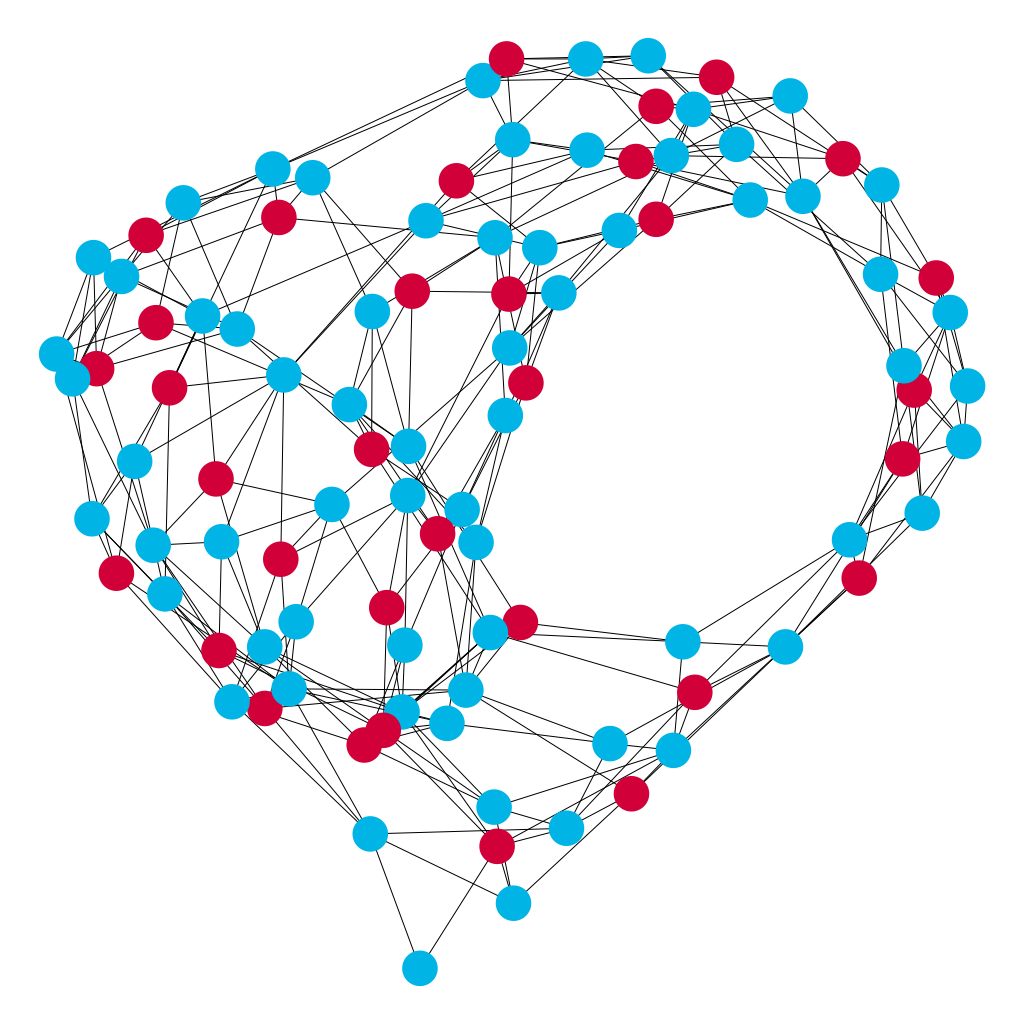
\includegraphics[scale=0.22]{imgs/Sim2E.png}
\caption{An interaction infrastructure where $\Delta(\Lambda)=0$ and $m=1.5$}
\label{Sim2}
\end{figure}

\subsubsection{Egalitarian exchange economy: Costly economic interaction}

The second set of simulations assume that there exists some costly inefficiencies for each economic interaction. Again, two simulations are conducted that correspond to the costless simulations above whereby the extent of the learning effects are altered. The first simulation assumes $m = 1$ and the second assumes $m = 1.5$. In both simulations we set the cost of forming an economic relationship at $\Delta(\Lambda) = 0.25$.

\paragraph{Simulation 1C : Costly interactions with equal learning effects.}

In the first simulation we find the existence of multiple equilibrium interaction infrastructures. One equilibrium is that of a monadic economy represented by an empty network, in which consumer-producers are indifferent to autarkically specialising in either $X$ or $Y$. In this case each consumer-producer earns a utility of $2$ in autarky. The other potential equilibrium is exactly the same as the first simulation in which pairs of economic interactions exist such that one consumer-producer specialises in the production of $X$ and the other specialises in the production of $Y$. Both equilibria are shown in Figure~\ref{Sim3}.

\begin{figure}[t]
\centering

\includegraphics[scale=0.22]{imgs/Sim3E.png}
\caption{An interaction infrastructure where $\Delta(\Lambda)=2$ and $m=1$}
\label{Sim3}
\end{figure}

\subsubsection{Cournot-Nash exchange economy: Costless economic interaction}

In these simulations we set $\Delta(\Lambda) = 0$. Prior to running the simulations we can note that, given the existence of an efficient trade mechanism where demand and supply are equalised, the use of a Cournot-Nash exchange mechanism leads to the following properties shown in Proposition~\ref{efficientSpec} below.

\begin{proposition} \label{efficientSpec}
Let there exist a Cournot-Nash exchange economy $\mathbb{E}_{C}$ such that $i,j \in N$. Assuming that $\Delta(\Lambda) = 0$ the following properties hold:
\begin{itemize}
	\item[(i)] All possible $ij$-interactions are mutually beneficial;
	\item[(ii)] The network that emerges is a complete network; and
	\item[(iii)] All consumer-producers are fully specialised in the production of a single output.
\end{itemize}
\end{proposition}

Proposition~\ref{efficientSpec} (ii) follows intuitively from (i), and Proposition~\ref{efficientSpec} (iii) is equivalent to Theorem~\ref{th:Spec}. The interaction network that emerges is analogous to a \emph{market} whereby all agents operate and trade with one another. Moreover, as interaction inefficiencies increase, the complete structure of the network can lose its integrity. This will be seen when considering the costly network formation below.

In the first simulation we set $m = 1$. As hypothesised in Proposition~\ref{efficientSpec} we find that a complete network emerges whereby agents that enter the socio-economic space specialise in a sequential manner such that agent 1 specialises in the production of $X$, agent 2 specialises in the production of $Y$, agent 3 specialises in the production of $X$, agent 4 specialises in the production of $Y$, and so on. The outcome of the simulation can be seen in Figure~\ref{Sim5}. We further note that the utilities of all agents converge.

\begin{figure}[t]
\centering
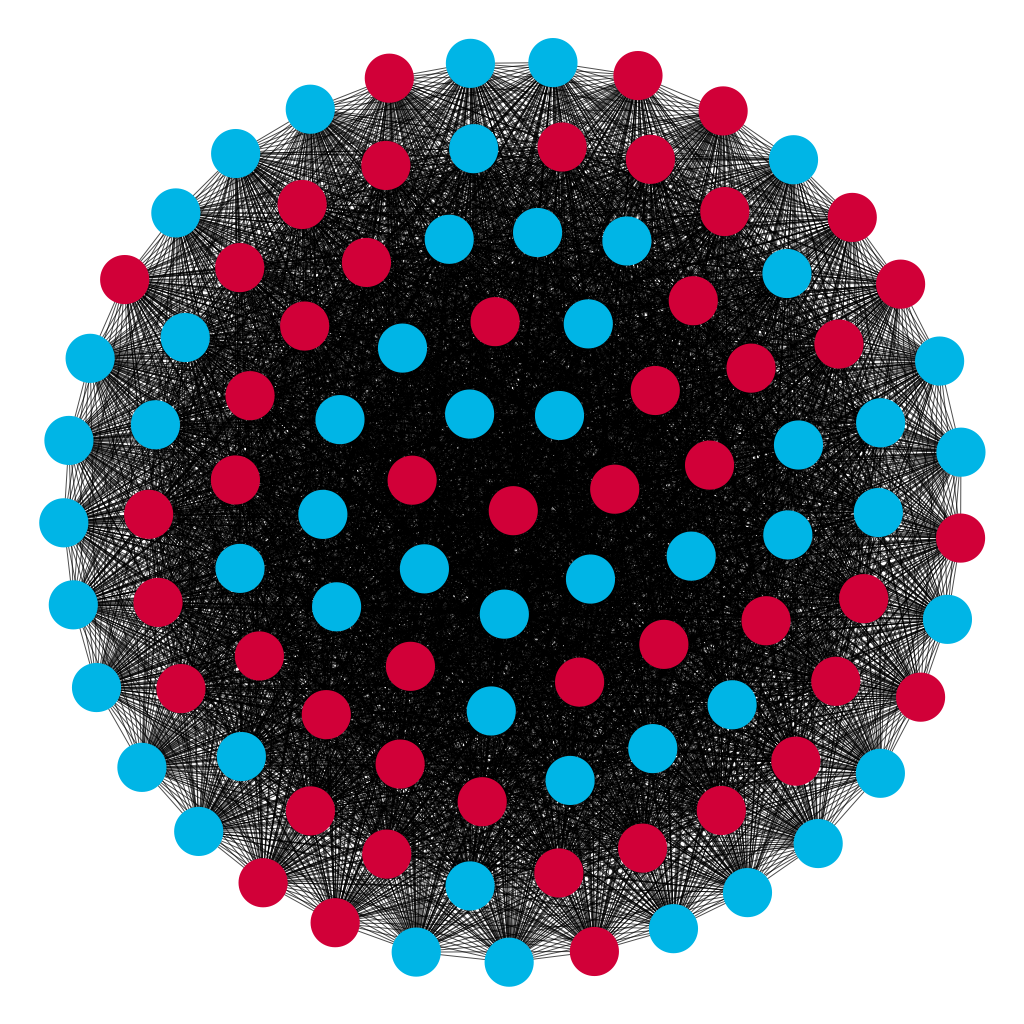
\includegraphics[scale=0.22]{imgs/Sim1C.png}
\caption{An interaction infrastructure where $\Delta(\Lambda)=0$ and $m=1$}
\label{Sim5}
\end{figure}

In the second simulation we set $m = 1.5$. Given that $\Delta(\Lambda) = 0$ the interaction inefficiency is minimal and thus a complete network is generated from the simulation of the Cournot-Nash exchange mechanism. Therefore, regardless of the production technology the topology of the interaction infrastructure remains unchanged. The only notable change is the proportion of agents specialising in the production of good $Y$, which increases due to the improved production abilities. Due to the lack of change with regards the structure we do not provide a corresponding Figure.

\subsubsection{Cournot-Nash exchange economy: Costly economic interaction}

The third simulation assesses costly network formation, in the form of positive interaction inefficiency, with equal production technologies for both goods $X$ and $Y$. We note that interaction inefficiencies are experienced on both sides of the economic interaction, not just the agent entering the socio-economic space and initiating the interaction. As a consequence, the network formation process follows a two-sided network formation model.

The result is the formation of a scale-free network with a degree distribution that follows a power law whereby the earliest entrants into the socio-economic space have the largest number of economic interactions. Due to the cost in forming economic interactions the and the production abilities of the individual agent the number of economic interactions per agent is limited unlike what was seen in the initial costless simulation, whereby the efficient price mechanism provided local price levels that benefited both parties when engaging in the economic trade. This limitation means that early entrants into the socio-economic space will engage in many exchanges as new agents enter the space; however, the number of their interactions will stop at some level. This will happen consecutively for all early economic agents thus leading to a structure with multiple hubs. These `hubbed' nodes are the earliest agents to enter the socio-economic space\footnote{We further note that a scale-free network is the natural market structure to emerge from adaptive specialisation. When simulating the emergence of an interaction infrastructure whereby agents could make only a limited number of economic interactions when entering the socio-economic space a scale-free network also emerged. A set limit on the number of economic interactions that can be formed forces individual economic agents to only form interactions with others that already have a large number of economic relations.}. Many empirical economic exchange networks also follow this scale-free structure \citep{Schweitzer2009}.

\begin{figure}[t]
\centering
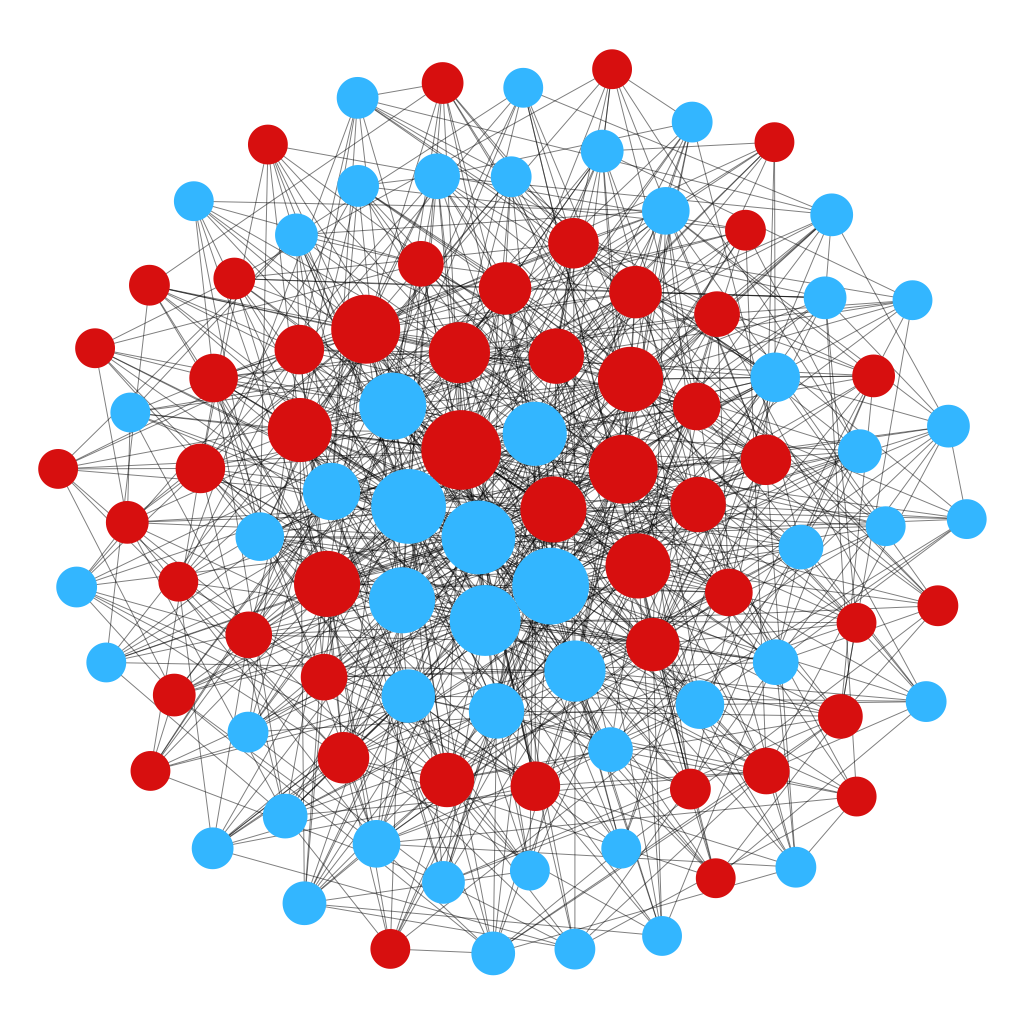
\includegraphics[scale=0.22]{imgs/Sim3C.png}
\caption{An interaction infrastructure where $\Delta(\Lambda)=0.2$ and $m=1$}
\label{Sim7}
\end{figure}

\subsubsection{Analysis of results} % (fold)
\label{sub:analysis_of_results}

% subsection analysis_of_results (end)

The representation between the interaction of elements of the socio-economic space shown in Figure~\ref{spacestructure} suggests that the institutions of a socio-economic space have a direct impact on the interaction infrastructures, which are formed by the economic interactions of a population of agents. The infrastructure is therefore a reflection of the state of the institutions and that entrepreneurship acts to alter the institutional environment, which is reflected in the interaction infrastructure itself. Our simulations of the socio-economic space based on the division of labour confirms the representation shown in Figure~\ref{spacestructure}. Specifically we model institutional and technological change in a number of ways. First, we note institutional change through changes in the interaction inefficiency, or transaction costs, of exchange between pairs of economic agents. In short we find that as the interaction inefficiency rises from $\Delta(\Lambda) = 0$ to some positive real number the number of \emph{structural holes} in the network increases and there emerges an increased distribution of utility throughout the network. These structural holes appear due to the reduced benefits of forming economic relationships with the entire population of agents. A natural consequence of the algorithm that solves the adaptive specialisation problem is that for all economic agents the next economic relationship formed will provide less benefit than the previous relationship: there is diminishing marginal benefit for each economic interaction. 

Whilst increasing the interaction inefficiency there will exist a tipping point whereby below this level of interaction inefficiency there will exist some wealth-generating relationships and above this tipping point there exists no economic relationships between agents. With regards the first egalitarian exchange economy: if $\Delta(\Lambda) > 0.25$ then an empty network will emerge; if $\Delta(\Lambda) < 0.25$ a minimally connected bipartite networks emerges; and if $\Delta(\Lambda) = 0.25$ then multiple equilibria can emerge as each agent is indifferent to forming an economic interaction with another agent. This notion of tipping points when regarding changes in interaction inefficiency has important implications for how we perceive the development of the socio-economic space. Indeed, substantial development may occur through punctuated events of tipping points. The structure of an institution may change thus facilitating a non-linear increase in the number of functional economic interactions and utility generated throughout the network.

When the interaction inefficiency tends to zero then there will exist a more homogenous socio-economic space such that each economic agent will derive a relatively equal utility and have a position in the networked structure that is structurally equivalent to all other agents in the space. For example, when the $\Delta(\Lambda) = 0$ for both the egalitarian exchange economy and the Cournot-Nash exchange economy each agent has the same level of utility and possess positions in the space that are structurally equivalent to all other agents. Thus, some agents may benefit more than others by maintaining the interaction inefficiency at a relatively high level.

Second, we note institutional change through changes in the exchange mechanism itself. Specifically we consider two exchange economies---the egalitarian exchange economy and the Cournot-Nash exchange economy---which obviously depends on the exchange mechanism used for trade. This is a more substantial change than simply a change in the interaction inefficiency experienced by agents to use the elements of the governance system to form economic interactions with each other. Moreover, a change in the exchange mechanism used may not lead to a change in the interaction inefficiency itself. Again, the exchange mechanism used has a substantial impact on the topology of the interaction infrastructure of the socio-economic space and the overall utilities of individual economic agents. The simulations showed that the use of a Cournot-Nash exchange mechanism was superior to the use of the egalitarian exchange mechanism in terms of the utility it generated for each individual agent.

Finally, we investigate change in the efficiency of production technologies through the variable $m$, which is connected to the efficiency regarding the production of good $Y$. An improvement in the production technologies of a given output may emerge from a reduction in role-building costs of the specific role that pertains to the output $Y$, or it may derive from an improvement of actual technological production. We find that as the efficiency of the production technology increases and agents become more productive in the production of good $Y$, more agents tend to specialise in the production of $Y$. Influencing a change to the production technology of some output leads to a change in the topology of the interaction infrastructure and the proportion of the population specialising in the production of the given output. Specifically, as $m$ increases, there will be more incentive for agents to specialise in the production of $Y$.

\paragraph{The impact of entrepreneurship.} % (fold)
\label{par:the_impact_of_entrepreneurship_}

% paragraph the_impact_of_entrepreneurship_ (end)

As noted in Definition~\ref{def:entrepreneur} above, entrepreneurship refers to the actions that modify in a major way elements of the governance system and the underlying interaction infrastructure of the socio-economic space. With respect to the simulations above, the transition from one exchange mechanism to another and technological advancements---the ability for individual economic agents to improve their production possibilities---relates to the process of entrepreneurship. 

We see that all institutional and technological changes discussed lead to major changes in the interaction infrastructure and society's utility. Both institutional changes---the reduction of interaction inefficiency for all agents and the change in the exchange mechanism used---are signs of entrepreneurial action. An improvement in production technologies can be more ambiguous if the change in production technologies is attributed to institutional changes itself. For example, if the improvement in production technologies is a consequence of a reduction in role-building costs for all agents due to, for example, the establishment of or improvement in educational institutions then this may be considered an act of entrepreneurship. If however, the improvement in production technology is isolated to the individual herself and not others in the socio-economic space then this will be considered the act of the entrepreneurial function. This conclusion regarding the regarding the scale of entrepreneurial action follows the same lines as Schumpeter, who claimed that an entrepreneur had a \emph{disequilibriating} impact on technological innovation. 

This short discussion of the entrepreneur and the resulting simulations provide an overview on the role of the entrepreneur and the impact of entrepreneurship within the relational perspective. Due to the importance of entrepreneurship and the lack of discussion and clarity on the topic of the entrepreneur in traditional economic literature we provide a further discussion in Chapter~\ref{ch:entrepreneurship}. In the subsequent discussion we draw an important link between the act of entrepreneurship and the generation of new socio-economic roles and unique, and potentially exploitative, positions within the socio-economic space.

\chapter{Entrepreneurship and the entrepreneurial function} 
\label{ch:entrepreneurship}

If the division of labour is at the centre of the relational perspective, then its evolution is of major importance in our discussion. Section~\ref{subsec:growthdev} noted that the development of a socio-economic space and the structure of the division of labour depends in some way on two factors; the first factor informs the division of labour and the other factor actively influences the composition of the division of labour. The first factor regards the architecture of the governance system that exist within the socio-economic space. The governance system--which consists of all embedded socio-economic institutions--informs the context of all economic interactions and relationships within the space, as well as socio-economic roles and production possibilities for individuals and firms. Therefore the division of labour, and thus the socio-economic roles attainable within society, is ultimately informed by the accepted governance system of the space. The second factor regards entrepreneurship, which influences a change to the socio-economic space by modifying elements of the prevailing governance system. Elements of the governance system can be influenced through entrepreneurial actions and the division of labour extended; an initial insight made by \citet{Smith1776}. Outlining a theory of the entrepreneur, and with it a theory of the entrepreneurial function within the relational perspective, is a main focus of this chapter.

After outlining a theory of the entrepreneur within the context of the relational perspective we illustrate the notions of entrepreneurship and the entrepreneurial function with an empirical example from history: the rise of the House of Medici. One of the most acclaimed pieces of business history is Raymond de Roover's investigation into the rise and fall of the Medici Bank. His analysis chronicled the evolution of the House of Medici from its establishment by Giovanni di'Bicci de'Medici, and later growth by his son Cosimo de'Medici. This case study approach, although deficient in overarching theory, provides an impressively intricate analysis of the financial accounts and business practices of the Medici Bank. The chapter therefore contributes to the work on the House of Medici by developing a theoretical overview of entrepreneurship and the entrepreneurial function and applying it to the actions of the entrepreneurial agents that drove the rise of the Medici Bank. Our specific application assesses the actions of Giovanni di'Bicci de'Medici and his son and heir Cosimo di'Giovanni de'Medici. Although much has been written regarding the rise and fall of the Medici Bank there are none, to our knowledge, that specifically apply general theoretical models of entrepreneurship to this case study.

This chapter follows an analytical narrative approach inspired by `new business history'. The focus of new business history, according to \citet{JongHigginsDriel2015}, is to complement the case study research with a theoretical foundation. The focus on single firms within business history is not the source of the methodological problems faced by business historians. Studying single firms may highlight the need for more general models. In a recent pa\citet{Brownlow2015} acknowledged the call of De Jong et al. for a new business history. In doing so Brownlow provides an analytic narrative regarding the establishment of the \emph{DeLorean Motor Company} in Northern Ireland circa 1975--1981, after the infamous `Troubles', a term associated with the ethno-nationalist conflict. Brownlow provides a convincing depiction of DeLorean as a rent-seeking entrepreneur who exploited Government policies and institutional responses to the deficient Northern Irish economy relative to the rest of Britain. The use of the analytic narrative illustrates the application of entrepreneurship is an important methodology, and one that we will use after outlining the entrepreneurial theory.

We take much inspiration from Brownlow and also note the call from De Jong et al. by investigating the Medici case with the proper methodology developed within the relational perspective. We provide an assessment regarding the entrepreneurial actions of the Medici Bank by investigating its establishment and prominence under the guise of institutional entrepreneurship. Specifically we provide a holistic perspective of entrepreneurship and the entrepreneurial function within a socio-economic space built from the basis of Schumpeter, Burt, Baumol, and Henrekson \& Sanandaji. By doing this we add some theoretical perspective to the business history contributions by de Roover and others regarding the rise of the Medici bank, the change in both the informal and formal perception of usury during this time, and the partnership system architecture of banking during this time. In undertaking this we cover institutional and entrepreneurial theories.

\subsubsection{Motivating an analytic narrative of the Medici}

The standard approach of economists in motivating an in-depth investigation is to formulate a set of puzzles. A number of interlinked puzzles can be identified when considering the establishment and rise of the Medici bank and the change in the institutional structure of Florence and Italy during this time. The first regards the institutional change regarding money-lending and the provision of financial credit that allowed it to move out of the ghettos in Florence to become the legitimate preserve of banks. This transition was symbolised by the rise of international money-lending and the rise of the Medici bank.

The second puzzle regards the phenomenal economic prosperity of the Medici bank and the political dominance of the Medici family across two generations of the family. The Medici family rose from obscurity to become one of the most powerful families in Europe. Prior to 1394---the establishment of the Medici bank---the Medici family were renowned criminals in Florence. Indeed, within a seventeen-year period five members of the Medici clan were sentenced to death by the criminal courts for capital crimes. The puzzles regarding the rise of the Medicean hegemony are addressed with respect to an analyses of entrepreneurship within the relational perspective; which regards economic actors who actively motivate a change to the governance system of the socio-economic space. In relation to this we look also to the interrelationship between the political and economic spheres of the economy, and how the Medici rose to dominate these spheres of the economy.

Beyond the economic puzzles noted, the motivation for analysing the Medici is related to the fact that there exists few other entrepreneurial families that have had such an impact on the cultural and economic composition of an Age than the Medici family. It is certainly debatable to suggest whether the world we see today would have been the same if the Medici had not come to such power in Florence during the late Middle Ages. It is of interest to see how a family gained so much economic and political control; how the actions and innovations of a small group punctuated the direction of a civilisation. More specifically, it is important to see how a model of the entrepreneur can explain how individuals attain power within a relational economy. The Medici were able to amass so much power and success due to their entrepreneurial ability: their potential to innovate, network, and create their own subjective socio-economic role within the Florentine socio-economic space enabled them to attain high levels of wealth and prestige.

\paragraph{Chapter outline.}

The first section provides an outline of the existing theory regarding entrepreneurship. The next section integrates the notion of entrepreneurship to that of institutions and the governance system. From this we combine our perception of the relational perspective with the entrepreneur to discuss a more holistic perspective of the entrepreneur and entrepreneurship within the relational perspective. The final section applies the notions developed to the case study of the rise of the Medici bank.

\section{Theoretical perspectives of entrepreneurship}

A classic perspective of the entrepreneur comes from the work of Frank \citet{Knight1921}. Knight's perspective claims that all forms of entrepreneurship must have `uncertainty' and `profit' involved. His central thesis suggests that entrepreneurs profit from the burdening of uncertainty. This notion of uncertainty corresponds to the definition it has been given throughout the thesis: uncertainty relates to one-off events whose probability and outcome can only be subjectively estimated. Unlike risk, uncertainty cannot be estimated and insured against. Profit is the reward for those willing to bear unmeasurable, inestimable and uninsurable uncertainty rather than measurable, estimable and insurable risk. Entrepreneurs are thus those who are willing to incur the uncertainty of a potentially profitable course of action. This distinction between risk and uncertainty typically does not, however, filter into traditional economic theory. As a consequence \citet[p.~282]{Knight1935} notes that, ``in the idealised society of equilibrium theory, there would be no occasion for assigning the distinctive name of profit to any type of return.''

Traditional economic theory has suffered in the past from a failure to state clearly the role and actions of the entrepreneur. The persistent words of William \citet[p.~66]{Baumol1968} summarise how traditional economics has investigated this elusive economic entity since the Marginalist Revolution: ``The theoretical firm is entrepreneurless--the Prince of Denmark has been expunged from the discussion of Hamlet''. The consequence of this discrepancy should be underlined considering that some economists believe the entrepreneur to be the driving force of the prevailing capitalist ideology and economic prosperity \citep{Schmitz1989, WennekersThurik1999, Baumol2007}. Further, \citet[p.~1]{Lazear2002} suggests that, ``the entrepreneur is the single most important player in the modern economy.'' This omission within mainstream economics is certainly perplexing given its apparent importance. 

This section investigates three established theoretical perspectives of the entrepreneur and entrepreneurship. The first is that of occupational choice models and models of endogenous growth developed within the neo-classical framework. The second is the Schumpeterian perspective of capitalist economic development through the waves of creative destruction spurred by the entrepreneur. The final perspective is the Burtian perspective of the entrepreneur, developed on the basis that all economic activity is embedded in a social network.

\subsection{Traditional economics and occupational choice}

Ultimately, Baumol's argument is that the traditional theory of the firm does not allow for the integration of the entrepreneur. The production function suggests that the firm considers the costs and benefits attached to the employment of certain and well-defined factors of production including capital and labour. All firms within the industry optimise and operate at their profit-maximising equilibrium and subsequently provide an inert market structure producing output that already has a market attached. In the extreme case of perfect competition, certainty, homogeneity, non-existent barriers to entry, and individuality are assumed. A paradox follows whereby at the equilibrium of perfect competition there is no competition: all firms operate independently earning normal profit without being given the opportunity to innovate or undercut rivals. Innovation, reorganisation of trade networks, the leveraging of unique social networks, and product or process diversification are cast out of the equilibrium model. The eventual failure of marginal firms only derives from an exogenous change in the market as opposed to factors of uncertainty, bad networking, or poor managerial decision-making due to bounded rationality.

To suggest that neo-classical economics has continued to disregard the entrepreneur since the words of Baumol would be incorrect. Jean Baptiste Say initially coined the term around the beginning of the 19th Century \citep{Hindle2008}, claiming that the entrepreneur was an economic agent who owned a large quantity of resources and allocated them out of an area of lower into an area of higher productivity and greater yield. To a large extent, this perspective has been embraced by the neo-classical models. Indeed, the models of static equilibria provided mechanisms in which to integrate the individuals' decision to be an entrepreneur as an `occupational choice', meaning that individuals allocated their entrepreneurial talents to either becoming an entrepreneur and set up their own (homogeneous) firm or becoming an employee for an existing firm depending on the prevailing market wage level to the corresponding actions. The models from \citet{Lucas1978} and \citet{KihlstromLaffont1979} form the foundations of entrepreneurship as an occupational choice for economic agents.

Some deficiencies of occupational choice models are due to their market-centric foundation and assumptions. Specifically, equilibrium theories of the entrepreneur make three main assumptions. The first being that every economic agent can recognise all entrepreneurial opportunities, which derives from their \emph{ex ante} homogeneity. The second is that fundamental attributes about people--rather than information about opportunities or the encompassing structure of the socio-economic environment--determines who becomes an entrepreneur. Although human action is the result of individual ability there is no doubt that external and social factors also play a role on determining entrepreneurial action \citep{ShaneLockeCollins2003, AldrichMartinez2007}. Finally, they have the perception that being an entrepreneur is an occupational choice: that individuals can just choose to be an entrepreneur or not. The relational perspective developed above notes that most individuals cannot just `choose' to specialise in the role of an entrepreneur. Rather, it will be seen that individuals create their own role--they subjectively specialise--to their socio-economic environment. Indeed, they do not adopt a pre-existing occupation, but rather create their own and thus spur the deepening of the division of labour.

Endogenous neo-classical growth models have been created which include the notion of the entrepreneur \citep{Peretto1998, Sanders2007}. The most influential of which is the \citet{AghionHowitt1992} model and its later adaptations \citep{Aghion1997, HowittAghion1998} which facilitates the integration of entrepreneurial innovation as a driver of economic growth. Indeed, they do this by having firms invest resources in research to achieve a new product that renders the previous product obsolete. Capital is excluded from the basic model while economic growth results from technological progress, being a result of competition among firms that generate innovations. Firms are motivated by the prospect of temporary monopoly rents after a successful innovation is patented. Another innovation will again destroy these rents, as the `entrepreneur' is making the existing good obsolete. Although these are highly influential models created by Aghion and Howitt, and capture the Schumpeterian notion of creative destruction, they fail to capture the characteristics of the agent that leads to the destabilisation of the economy through the process of creative destruction--the entrepreneur. Indeed, although the 1992 article, for example, regards creative destruction as a driver of growth they do not mention the word ``entrepreneur'' throughout the article. Instead they simply suggest that it is the firm, investing in research and development, which drives technological advancement and therefore economic prosperity. This is undeniably true; firms that invest in research and development can create innovative products, but innovation still emerges from sources external of the firm. Again and again, it is seen that the neo-classical models' attempts to capture the entrepreneurial functions are continually ill-equipped.

The development of entrepreneurial models specifically built with the intention of encompassing institutional and social aspects are of paramount importance as the ultimate role. The perspective we develop of the relational entrepreneur will depend on the structure of the socio-economic environment. To this point we have seen that mainstream theory finds it difficult to model economic evolution through the entrepreneurial function. Below we will point to potential reasons why the mainstream theory finds it difficult to appropriately model economic evolution through the actions of the entrepreneur. I suggest that the problems of the traditional theory derive from the very axioms that underpin it: methodological individualism, methodological instrumentalism, and methodological equilibration. First we must extend our discussion of how economic theory perceives the entrepreneur by discussing the Schumpeterian and Burtian perspectives. From this basis we integrate institutional factors into entrepreneurship and provide a discussion of entrepreneurship within the relational perspective.

\subsection{Schumpeterian theory of the entrepreneur}

Although being progressively side-lined over previous decades \citep{Aldrich2005}, one of the most prominent perspectives of the entrepreneur comes from Joseph Schumpeter who discusses the entrepreneur and the entrepreneurial function in two places: the first is in chapter two of his book on economic development \citep{Schumpeter1934}; and the second is in a chapter prepared in 1928 for an economics handbook \citep{Schumpeter2003}. Schumpeter provides a novel perspective of the entrepreneur that is fundamentally differentiated from the neo-classical postulations. Realising the limitations of general equilibrium analysis in explaining economic evolution and development, Schumpeter rejects any notion of equilibria, instead emphasising that the economy needs to be analysed in a purely dynamic manner propelled by the waves of `Creative Destruction' \citep{Schumpeter1942}. From this basis he built a relatively loose conceptual model on the premise that even if markets were to approach equilibrium they would destroy it over time due to the advancement of product and process innovation. Through the entrepreneurial function new products and markets would be created thus provoking a deviation from the equilibrium point and the circular flow of the economy. The process of creative destruction as discussed by Schumpeter assumes that all entrepreneurial activity progresses the capitalist economic system; that the entrepreneur is a heroic entity productively influencing production and process techniques and providing new technologies and specialisations to the socio-economic space.

\subsubsection{Entwicklung and the entrepreneur}

Schumpeter's overall perspective of the entrepreneur fundamentally deviates from neo-classical economics, and thus Say's contribution of an individual that allocates resources in a more efficient manner. Instead, he initially took a more literal definition of the term entrepreneur as an individual who stimulated economic progress by finding new and better ways of doing things. In doing so Schumpeter emphasises the importance of innovation--a dynamic process that emerges from a stagnated state of affairs so that a new state of affairs can emerge--a concept notably absent from the neo-classical models of comparative statics, where the types of goods and services are given. Even the goods and services in the future are fully specified, which allows for inter-temporal trade. Production technology is also given. However, in emphasising innovation he took a relatively social perspective of the entrepreneurs' socio-economic environment. Moreover, he fully accepted that not every agent could be an entrepreneur. Each entrepreneurial agent specifically required two resources. The first resource was the existence of technical knowledge in order to produce new, innovative, outputs. Second, they required the power of disposal over the factors of production in the form of credit. In effect an entrepreneur requires specific forms of human capital for the development of relevant innovations, and also the sources of credit to fund its development and diffusion with the use of markets.

Considering this innovative and mutative quality, Schumpeter's acceptance of evolution--or \emph{entwicklung} \citep{Schumpeter2005}--is particularly notable. However, despite flirting with the concept of selection, Schumpeter did not follow his insights up with any major evolutionary discussion \citep{SmelsterSwedberg2005}. Further still, despite his efforts, he failed to provide any formal model in which to specifically link the entrepreneur, the entrepreneurial function, creative destruction, and economic development \citep{Witt2002}. He did however attempt to conceptually couple his discussion of the entrepreneur with one of internal economic development. He specifically saw that development was a process that emerged from actions endogenously occurring within the economy itself and not from the impact of some form of exogenous shock. An economy that was simply adapting to shocks that were exogenously endowed or were external to it was perceived as simply being dragged along by the changes in the surrounding world. This adaptation to an external or exogenous factor is not development. According to Schumpeter, economic development comes from innovative entrepreneurial action within the economy itself.
\begin{quote}
By `development' we shall understand only such changes in economic life as are not forced upon it from without, but arise by its own initiative from within... By this we should mean that economic development is not a phenomenon to be explained economically, but that the economy, in itself without development, is dragged along by the changes in the surrounding world, that the causes and hence the explanation of development must be sought outside the group of facts which are described by economic theory.

\begin{flushright}
Joseph \citet[p.~63]{Schumpeter1934}
\end{flushright}
\end{quote}
Despite his efforts to integrate the entrepreneur to endogenous economic development, Schumpeter largely failed to do so. As \citet{Becker2006} point out in the introduction of Development \citet[p.~111]{Schumpeter2005}, ``Development's dismissal of entrepreneurship as the explanation of discontinuities is the rare instance where Schumpeter himself indicates that he is still searching for an entirely adequate explanation of the novel social phenomena he had characterized as discontinuities.''

In discussing economic development, Schumpeter was adamant that development was not a self-organising process. Specifically he suggested that, ``[t]he economy does not grow into higher forms by itself'' \citep[p.~75]{Schumpeter2003}. When considering situations of increased complexity the difficulty of self-organisation becomes notable. Subsequently it becomes apparent that the entrepreneur does not just act as a diffuser of an innovation, but acts as an organising force that drives development of an economy from inside \citep{Marz1991}. Entrepreneurs actively organise society and the divisions of labour in the production of innovative outputs. With this, Schumpeter makes an interesting argument that homogeneous and fully autonomous agents may not necessarily produce systems that organise successful development when considering complex economies. Forces in terms of the entrepreneur and the government must actively organise society in fruitful production. Even if this organisation is imperfect or lacking fruitful development can still emerge.

\subsubsection{Personalisation and depersonalisation of the entrepreneur}

There remains an amount of controversy as to whether his perspective of the entrepreneur changed over time. There does seem to be an implicit distinction between what Schumpeter considered to be the entrepreneur, and what he considered to be the entrepreneurial function. However, his views on these are not mutually exclusive, he simply views the same innovative process from two different perspectives. In his latter work, Schumpeters analysis was extremely depersonalised, focussing on the process and outcome of the entrepreneurial function within the economy. In doing so, Schumepter placed more of an emphasis on the entrepreneurial activities and actions as opposed to the entrepreneurs' personal characteristics. \citet{BeckerKnudsen2003} implied that this made entrepreneurship seem to be a much more contingent activity; that the entrepreneurial function did not have to specifically emerge from a single individual, but may emerge from a group activity or a firm.

With respect to the depersonalised entrepreneurial function, Schumpeter stressed that the function of the entrepreneur is to reform or revolutionise the pattern of production. They can do this in many ways: by exploiting an invention or, more generally, an untried technological possibility for producing a new commodity or producing an old one in a new way, by opening up a new source of supply of materials or a new outlet for products, by reorganising an industry and so on. From this definition it is seen that the Schumpeterian entrepreneur is extremely firm-centric; providing the linkage specifically between the innovative function and firm organisation and output. Despite the difference in approaches, Schumpeter - like the neo-classical paradigm - stresses a direct link between the development of technology and resulting economic prosperity. However he suggested that technological advancement came from the fruition of an entrepreneur's innovative idea embodied within the economy and the production of heterogeneous output as opposed to a mere exogenous shock. This provides a general consensus that the entrepreneur is considered as an entity which blurred the distinction between macro and macro spheres of the economy: the entrepreneurial function was a microeconomic action with potential macroeconomic implications.

Under this definition Schumpeter contended that the entrepreneurial function, and thus the acts required to become an entrepreneur, was not the same as choosing an occupation or a profession. It is specifically not an occupational choice; one cannot learn to become an entrepreneur as if it were any other profession. To be an entrepreneur an agent must specifically carry out an innovative process, which is outside the predefined actions of a socially expected role. Thus being an entrepreneur is specifically converse to simply following the established institutions and subsequently conforming to a specific socio-economic profession. Moreover, Schumpeter contested that one should not be considered to be an entrepreneur forever; an entrepreneur should only be considered to be so during the period in which the agent is carrying out the innovative entrepreneurial function.

Schumpeter's earlier work looked more at the characteristics of the entrepreneur, or the `man of action', as an entity. In this text he considered the entrepreneur to be an exceptional, disruptive individual who actively \emph{disequilibriates} the economy with the introduction of new products or processes, thus carrying out the aforementioned entrepreneurial function. It is emphasised that entrepreneurial success is derived from the utilisation of an exogenous skill-set. In his first rendition of the entrepreneur he attributes almost superhuman powers of leadership to the entrepreneur. In many ways, he perceives the entrepreneur as an agent with innate talent; indeed, what differentiates a successful entrepreneur from other agents within the economy is their ability to lead a firm or act on an innovation. Much like the Lucas model, the entrepreneur is psychologically endowed with a form of `talent' or `leadership' that is exploited for successful entrepreneurship. In all, the exogenously endowed characteristic attributes of Schumpeterian entrepreneurs are claimed to be initiative, authority, imaginative foresight, leadership, best personified by the figure of a `promoter', a `captain of industry' (as long as he or she is innovative) as opposed to the `plain businessman' or manager who only does business as usual.

Within his perception of the entrepreneur, Schumpeter proposes a distinct dichotomy between inventor and entrepreneurial innovator as follows:

\begin{quote}
Economic leadership in particular must hence be distinguished from ``invention''. As long as they are not carried into practice, inventions are economically irrelevant. And to carry any improvement into effect is a task entirely different from the inventing of it, and a task, moreover, requiring entirely different kinds of aptitudes. Although entrepreneurs of course may be inventors just as they may be capitalists, they are inventors not by nature of their function but by coincidence and vice versa... It is, therefore, not advisable, and it may be downright misleading, to stress the element of inventions as many writers do.

\begin{flushright}
Joseph \citet[p.~88--89]{Schumpeter1934}
\end{flushright}
\end{quote}

Given this, an inventor was seen to be a person that creates the new product or process, but does not necessarily distribute it throughout the economy. On the other hand, an entrepreneurial innovator is a `leader' who economically commercialises, puts into practice, and distributes an invention through his own labour. Therefore it is the innovator, as opposed to the inventor, who provides the shock to the economy and thus initiates the process of Creative Destruction through the entrepreneurial function. At the time, Schumpeter suggested that the inventor and the innovator would be two distinct entrepreneurs; however he still noted possible situations when the inventor role may coincide with the innovator. Although these situations were not considered to be typical, instead they were seen as mere exceptions to the rule. So, importantly, Schumpeter's analysis highlights that the innovating entrepreneur does not necessarily have to be the one that creates the novel product or process, but rather uses his superior networking abilities to distribute the innovation throughout the relevant economic network. Most notably, although attempting to depersonalise the entrepreneurial process in his later work, Schumpeter still must suggest that the successful entrepreneur is endowed with some form of exogenous leadership talent, which leads to the diffusion of the innovation and the ultimate disequilibriation of the economy.

Within his analysis of the entrepreneur Schumpeter provides a number of insightful notions. Not only does he put forward the concept of creative destruction, which is propelled by innovation through the entrepreneurial function, but he also provides an insight as to where this innovation is likely to emerge: through new production processes and the distribution of new products. The fact that he must provide such an exogenous psychological characteristic to explain successful entrepreneurial action through superior leadership, much like in the occupational choice models, is one of the major deficiencies of Schumpeter's theory of the entrepreneur, and one that was noted by other economists of his time. For our purposes we claim that the Schumpeterian perspective of the entrepreneur is deficient in two main ways. The first deficiency notes the lack of socio-economic institutions; which is indicated and partially remedied by \citet{Baumol1990}, and is discussed in detail below with reference to the socio-economic space. We therefore postpone the discussion with respect to the impact of the rules of the game to Section~\ref{entrepreneurshipInstitutions} below. 

A further deficiency is that Schumpeter did not take into consideration the foundational networks of entrepreneurial activity. His ideas are still ingrained in the theory of markets as the interaction of household preferences and firm production functions. Indeed, it is suggested that an entrepreneur needs to be well placed in order to collect and disseminate ideas and resources. This is a relational feature that is present with respect to Ronald Burt's perspective of the entrepreneur. Burt provides a sociological theory in which to perceive the entrepreneurial function. Although not discussing innovation and invention directly, this sociological perspective may be able to be complimented with the Schumpeterian perspective in the development of ideas and the initiation of creative destruction from a positional and relational aspect.

\subsection{Burtian theory of the entrepreneur}

Whereas the Schumpeterian entrepreneur explains economic development through product and process innovation, The theory of Ronald \citet{Burt1992, Burt2005, Burt2010} discusses the act of entrepreneurship on the basis of the social structure that underpins economic activity. This perspective is based on the premise that economic processes operate on the basis of social ties, and are therefore socially embedded. As a consequence, and keeping in line with other economic sociologists, development occurs not just from the process of Schumpeterian innovation, but it also occurs from the reorganisation and exploitation of positions within social networks. Specifically, Burtian entrepreneurs are individual agents that benefit from exploiting bridge relations that span structural holes of a social network or architecture of an economic organisation.

The notion of the Burtian entrepreneur builds on the inherent topology that naturally emerges within society. All social structure is comprised of a large number of triadic clusters with weak ties bridging them. This structure is illustrated by the small-world, scale-free, and hierarchical network structures discussed in Section~\ref{sec:socialeconomicnetworks} above. Indeed, all three common network topologies have the characteristics of an above-random clustering of nodes and weak ties between those clusters of nodes. Burt's line of discussion follows that of \citet{Granovetter1973} in that weak ties refer to relationships that are `structurally' weak, such that they are not socially embedded. The removal of weak ties, for example, can separate two or more clusters of nodes by a substantial distance when removed; the removal of strong ties does not suffer from this problem. Indeed, the removal of a strong tie between a pair of nodes still means that the nodes can connect to each other through a path length of 2. Although ties can be weak in the structural sense, they are strong with regards the quantity and quality of information that they are able to transmit from one agent to the other. Strong ties, on the other hand, are weak with regards the diversity of information that can flow along them. Weak ties have a lack of redundant information that comes with the connection of cohesive and structurally equivalent contacts when strong ties are formed.

\subsubsection{Network bridges and structural holes}

At the basis of the Burtian entrepreneur is the notion of a \emph{network bridge}. The network bridge concept is defined as a link which, if removed, would cause two groups or cliques of nodes to become disconnected. As a consequence the geodesic distance between pairs of nodes between the two groups to be infinity. High levels of geodesic distance between agents represent holes in the socio-economic network of the space, and these structural holes create a competitive advantage for individuals whose relationships span the holes and therefore solely connect multiple hitherto components and facilitating relational transaction between the two groups. These positions are network bridges meaning that the entrepreneur acts as a gatekeeper. The notion of a network bridge, and thus a structural hole, can be seen diagrammatically in Figure~\ref{fig:networkbridge}. In this network the network bridge is given by the red link. There are structural holes throughout the network, they exist where there is some lack of links between any pair of nodes and can therefore be seen in the dual network.

\begin{figure}[h!]
\centering
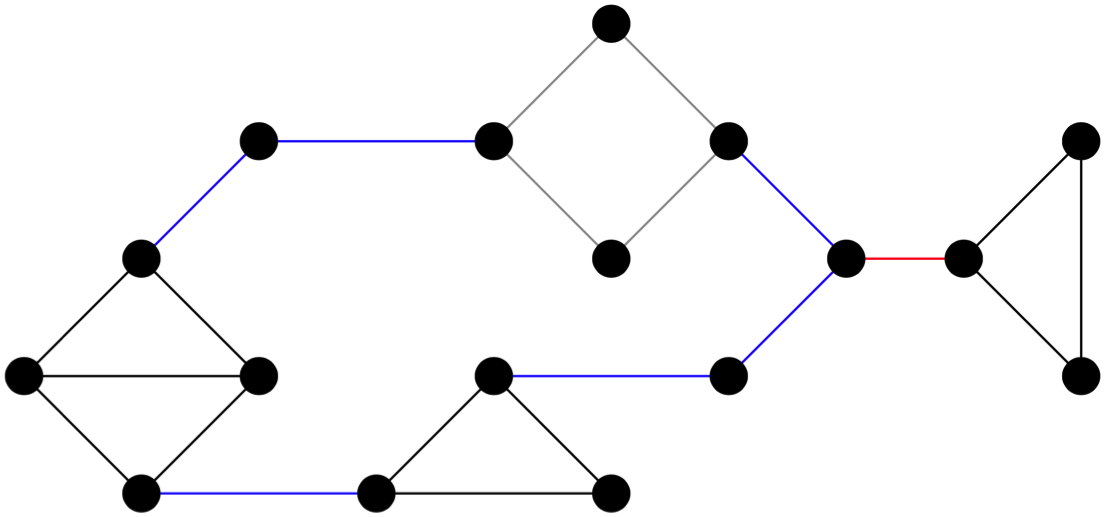
\includegraphics[width=0.85\textwidth]{imgs/networkbridge.png}
\caption[Strong ties, weak ties, and network bridges]{Network highlighting a network bridge in red, structurally weak ties in blue, medium strength ties in grey, and strong ties in black.}
\label{fig:networkbridge}
\end{figure}

Although Burts' theory focussed on an individual as opposed to a firm or other non-personal entity, there are perfect examples of institutions and other non-personal entities which act as network bridges or middlemen. These include financial institutions and firms such as Google and eBay. Indeed, eBay acts as a network bridge, or a middleman, between groups of buyers and sellers. In doing so, the agent reduces search costs (or more generally, transaction costs) between the two otherwise unconnected groups of individuals and receives network effects from the increasing use of eBay from both buyers and sellers. Because of the structural location of a Burtian entrepreneur, they could simply be seen as a market-maker, and thus a direct middleman of relational interaction and trade.

The network bridge theory of the entrepreneur does not explicitly express the creation of new products, processes or professions in society. It is simply a story of arbitrage and resource allocation through the entrepreneurial function. However, the dissemination of information and the exchange of ideas are typically required for the development of new technologies which can be easily integrated into this perspective. Indeed, it is notable that Burt's postulation did not come to an end with providing the positional theory of the entrepreneur. He extended the structural hole theory in a more philosophical and less formal way; primarily focusing on the generation of new, innovative ideas \citep{Burt2004}.

The core of his argument was that agents with bridge relations are critical to learning, creativity, and dissemination. Agents whose set of links span structural holes have unique access to diverse and even contradictory information and interpretations provides them an advantageous opportunity in forming and exploiting good ideas. Undoubtedly, ideas come from a variety of sources, divisions of labour, and over a variety of paths; but idea generation at some point involves moving specific knowledge and information from one group to another, bringing agents together, or combining knowledge across groups. This process of the entrepreneur alludes not just to the brokerage of information, but rather to the arbitrage, recombination and practical application of specific knowledge and information; the result of which may lead to the formation of a new firm. Burt furthers his proposition by suggesting that agents who have network bridges across multiple structural holes and multiple divisions of labour are more likely to have their ideas evaluated \citep{Burt2005}. Indeed, social networks are amazing tools for filtering and criticising good ideas--with more people evaluating an idea there is a greater chance for a good idea to emerge. Moreover, value accumulates as an idea disseminates. Value accumulates as an idea moves through the social structure and divisions of labour; each transmission from one group to another has the potential to add value. This idea dissemination allows for the creation of a tight feedback loop, which is needed for successful invention.

Therefore, people whose links span multiple network groups have a competitive advantage in the creation of good ideas. An idea in one group may be extremely valuable in another. An idea is only really valuable to agents and entities when the audience credit it with being. This is more likely when ideas are diffused, discussed, and evaluated throughout society. Although Burt did not discuss it, this idea generation by spanning multiple networks could be the beginnings in which to investigate the disruptive Schumpeterian entrepreneur.

\section{Entrepreneurship in the relational perspective}

The established theories are of two main strands. The first describes entrepreneurial actions that are shorn of institutional surroundings but respect the importance of positional opportunities. The second describes the relationship between institutions and entrepreneurship, which we discuss immediately below. Institutions are seen to provide the relative payoff structure that guide entrepreneurial actions and thus affect the allocation of entrepreneurial talent. Further, entrepreneurial activities can impact the context of institutions and the incentives that they provide to the economy as a whole. Such theories complement the relational perspective; specifically, the theories follow the directions of the schematic given in Section~\ref{subsubsec:schematicRepresentation} of the dissertation. 

An important, and often missing, component is the acceptance that productive entrepreneurship stimulates an extension of the division of labour and facilitates increased specialisation---as discussed by \citet{Smith1776}. This leads to the development of new socio-economic roles, new exchange architectures, and new forms of interaction. This reengineering of the socio-economic space provides the basis for greater interactions and the development of new innovations. A feedback loop between the extension of the division of labour and entrepreneurial activity is implied. Entrepreneurship actively deepens the division of labour by both directly and indirectly providing more socio-economic roles through the alteration of the elements of the governance system. This is done through, for example, the provision of new products or processes or the reconstruction of exchange networks and the reorganisation of trade---much like the Schumpeterian perspective. By using the established theories of the entrepreneur we provide an integration of the notion of entrepreneurship to the relational perspective discussed. The focus in this section is on the interaction between entrepreneurs and the governance system, and how their activities generate new positions within the socio-economic space. We first elaborate on how institutions impact the incentives and actions of economic agents.

\subsection{Institutions and entrepreneurship} \label{entrepreneurshipInstitutions}

The governance system contains all established socio-economic roles within society and therefore defines the depth of the division of labour. Further, the structure of the accepted governance system and institutions provide relative payoffs to society and coordinate a socio-economic space of interacting agents to some steady state. The notion that institutions guide agents to some equilibrium is not a new phenomenon. It is well accepted in many schools of economic thought that institutions provide the payoff structure of society: that agents follow the payoffs provided by institutional frameworks, and that the rewards are generated by the actions correlate directly to institutional frameworks.

\subsubsection{Institutional impact on entrepreneurship}

Entrepreneurial activities are affected by the incentive structure provided by governance systems and institutional frameworks. One of the most influential discussions regarding the relationship between institutional environments and entrepreneurship derives from \citet{Baumol1990}. Baumol contests Schumpeter's perspective on the entrepreneur: that the entrepreneur is an individual who productively drives economic development and prosperity through waves of creative destruction. Baumol instead observes that the distinct form of entrepreneurship within a society is determined by the institutional structures of that society; and thus integrates institutional structures into the analysis of entrepreneurial action. Baumol's suggestion is that some institutional environments and arrangements, which provide their set of payoffs have historically been more compatible with productivity-increasing technological innovations than others, however notes that entrepreneurship has historically not always been of the productive variety. Institutions tend to determine both the level and type of entrepreneurship and Baumol identifies three types: productive, unproductive and destructive. Institutional pathologies may ensure that payoffs are skewed towards rewarding redistribution favouring sectional interests rather than in return for productive entrepreneurship. Dysfunctional institutions, those that they are ill-defined or provide poor incentives, may provide a basis for entrepreneurs to exploit. These institutional frameworks may provide incentives for entrepreneurs to rent-seek--lobbying for barriers to entry or exploiting employment loopholes--as opposed to expending resources into more productive and socially beneficial endeavours. Institutions may be operating with such malfunction that they are created only to be exploited by entrepreneurs that will ultimately damage the wider economic performance of the economy.

Others have extended Baumol's insights in more general terms. \citet{Murphy1991} is concerned with the allocation of talent within an economy and the impact that this has for economic growth. The authors are interested in how the most talented choose to seek returns and how incentives in a society promote rent-seeking or profit seeking. As such, they introduce factors that encourage rent seeking and productive entrepreneurship. Productive entrepreneurship, much like Baumol's discussion on the issue, requires large markets for goods, good communication and transportation infrastructures that facilitate trade, low barriers to entry and expansion, accessible capital markets and sources of finance, clear property rights, patent protection, and an ability to start firms that can make rents on talent. Again, talented individuals are, due to their embeddedness, assumed to abide by the institutional framework and respond appropriately to them. \citet{Acemoglu1995} extends the thesis posed by Baumol and the work of Murphy, Schleifer and Vishny by finding that the reward structures that determine the allocation of talent are endogenous. The endogeneity of this allocation of talent allows for the existence of path dependency such that initial differences in rewards and/or allocations will have long-run effects as allocations of one generation shape the rewards for the next. In concluding Acemoglu argues that there can exist situations in which two-way causality between the rewards structures of society and the allocation of talent. Indeed, these may occur in some historical examples.

\subsubsection{Interaction between institutions and entrepreneurship}

The schematic provided in Figure~\ref{spacestructure} claims that entrepreneurship works to affect the institutional environment of the economy, and thus works in the opposite direction of embeddedness. Institutional frameworks provide the payoff structures for individual agents; which ultimately provides a reinforced equilibrium for the society of agents. Institutions form an embeddedness that is unidirectional; abiding to pressures and payoffs from an existing set of institutions is the opposite of how entrepreneurship is perceived within our framework. As a consequence, we would contend that Baumol's perspective is not a perspective of the entrepreneur, and thus entrepreneurship, at all. We come to this contentious point due to two broad reasons. First, Baumol does not appropriately define what entrepreneurship is within his remodelled framework. The actual role of the entrepreneur is unclear. Of course, this is not necessarily a deficiency of Baumol's work as it is of notable debate in entrepreneurship literature as a whole. Second, Baumol perceives the entrepreneur as an agent that responds to the payoff structure defined by institutional pressures without actively altering the environment in which they operate. 

With regards the second point, Baumol's analysis indicates that institutions can determine the balance between productive, unproductive, and destructive actions undertaken by entrepreneurs. However, as noted by public choice theory and as was indicated by Acemoglu's work, feedback loops can exist whereby opportunistic individuals can actively alter the institutional environment they operate in to improve their own payoffs. This is indeed the essence of entrepreneurship illustrated in Figure~\ref{spacestructure}. Entrepreneurship acts in the opposite direction of embeddedness: entrepreneurs modify the institutional environment that they operate in; the outcome of which can lead to positive outcomes for themselves, and potentially for society as a whole. Whether the entrepreneurial agent alters the governance system in a productive or unproductive way will largely depend on the institutions already in existence within the economy.

This interaction between institutions and entrepreneurs is somewhat captured in the work of \citet{HenreksonSanandaji2011} who integrate James Buchanan's insights into Baumol's model of the entrepreneur. \citet{Buchanan1980} noted that entrepreneurs can affect institutions in multiple ways, by: 
\begin{itemize}
\item[(i)] Market innovations that alter institutions or the effect of institutions; 
\item[(ii)] Evasion of institutions; and 
\item[(iii)] Direct political entrepreneurship. 
\end{itemize}
Just as Baumol noted that the supply and allocation of entrepreneurial talent depends on the institutional framework of society and therefore the relative payoffs to profit seeking and rent-seeking activities, Henrekson and Sanandaji note that the allocation of entrepreneurship depends on the ability for agents to abide, evade, or alter institutional frameworks. Moreover, they acknowledge that the same individual can switch between different forms of behaviour.

This bidirectional relationship extends Baumol's perspective and leads to the notion of \emph{institutional and political entrepreneurship}. This is not a new notion as discussed by \citet{BoettkeCoyne2009}. Initially, \citet{Dahl1961} discussed individuals who recombine resources in an effort to bring about change in policies that effect the wider economy. Within Dahl's framework, political entrepreneurs are effectively Schumpeterian entrepreneurs acting within the political space. A distinction is made between so-called political entrepreneurs and market entrepreneurs, who, ``refer to traditional Schumpeterian entrepreneurs, distinct from political entrepreneurs'' \citet[p.~50]{HenreksonSanandaji2011}. The authors claim that not only is there a distinction between these types of entrepreneur, but that they are interdependent: political entrepreneurs must create the environment for market entrepreneurs. The economic system can thrive or collapse as an outcome of the actions provided by political entrepreneurship. \citet{Eisenstadt1980} and \citet{HwangPowell2005} discuss `institutional entrepreneurship' which involves entrepreneurship over the structure of government--i.e., decisions regarding the general institutions within which ordinary politics take place. Institutional entrepreneurship specifically involves changes to the fundamental constitution of the formal and informal rules of the game. \citet{DiMaggio1988} used the term institutional entrepreneurship in reference to those individuals who have the resources and ability to generate changes in institutions. Institutional entrepreneurs can be driven by a variety of factors including monetary gain, prestige or power. This discussion of the entrepreneur extends beyond the political sphere of the economy, and focuses on more ingrained institutional features, such as informal rules of the game, including beliefs, behavioural rules, religion, and scientific knowledge. Such institutional entrepreneurship may have a less obvious but more distinct and withstanding impact on society \citep{Abrutyn2013}.

In all there is some consensus regarding the phenomenon that entrepreneurs can impact the institutional architecture of an economy, whether that be from the political or the economic spheres of the economy. The impact of an entrepreneurs' actions on the institutional architecture can be either productive or unproductive depending on the payoffs of conducting these acts. A productive entrepreneurial impact provides an environment with greater market opportunities and subsequent wealth-generation within society, but requires the incentive structure for entrepreneurs to provide it. An unproductive or destructive entrepreneurial impact conversely provides an environment with more restricted economic activities and opportunities, where talent is allocated to rent-seeking as opposed to profit-seeking acts.

\subsection{The unique network positions of entrepreneurs}

In properly integrating the entrepreneur and entrepreneurship into the relational perspective we provide a discussion on the interaction between entrepreneurship, institutions, and the unique positional attributes that economic agents attain from the development of a new socio-economic role within the division of labour. Below we provide a deeper insight into entrepreneurship and the entrepreneurial function within the relational perspective by understanding the interdependencies between the advancement of socio-economic roles, the development of positional attributes, and the context of the institutions of the governance system.

\subsubsection{Entrepreneurship, new socio-economic roles, and unique positions}

Chapter~\ref{ch:relationalperspective} argued that the development of a social division of labour leads to the formation of social and economic positions, given by Lemma~\ref{con:positionalattributes}. This is due to the network of relationships that form as a consequence of an individuals' specialisation and subsequent trade relationships. As such, individual economic agents will have a tendency to form similar socio-economic relationships given that they have similar socio-economic roles; there is positive assortativity in social and economic networks. We can therefore stipulate that--due to the the positional attributes of socio-economic roles and the novel nature of entrepreneurship--the formation of new socio-economic roles leads to the formation of a unique set of socio-economic relationships and thus a unique position within the socio-economic space. The uniqueness of an entrepreneurs positional attributes and the development of these unique positions fits well within the relational perspective and integrates some aforementioned theories of the entrepreneur; such as those from Smith, Schumpeter, and Burt.

Entrepreneurs therefore have access to higher levels of social capital with regards the formation of global and local bridges. Moreover, in extending Burt's insight we note that the entrepreneur adds value to this unique set of relations through entrepreneurial actions: specifically through the provision of an innovative output or production process that requires a hitherto unrelated set of specialisations and socio-economic roles; or through the potential rent-seeking and increased bargaining power that comes with brokering information and outputs. In some cases the entrepreneurial socio-economic role has some incentive to allow information to flow through the entrepreneur to other agents and specialisations; particularly with the formation of a novel output and the generation of ideas. In other cases, the entrepreneurial socio-economic role has some incentive to block the flow of information from one agent to the other; this may be the case where the exchange of knowledge does not directly benefit the entrepreneurial agent, or where the agent wishes to exploit some bargaining power to influence the institutions of society. The inherent institutional structure may affect the strategies of entrepreneurial agents; the governance structure of the space determines the actions of the socio-economic role.

\subsubsection{The interaction of institutions and network positions}

We have expressed two aspects of entrepreneurship thus far. First, the process of entrepreneurship can lead to the development of new socio-economic roles. As the division of labour deepens potential specialisation is extended and new positions are formed within the socio-economic space. Second, entrepreneurial agents form unique positions within the connected fabric of the socio-economic space, due to their positional attributes they can either be rent-seeking or wealth-generating with their actions. \emph{Middlemen}, for example, can exploit their position within a network through the process of rent-seeking or can facilitate exchange between individuals and markets that were previously unconnected by providing a platform for interaction. Consequentially, entrepreneurial agents can act in a positive-sum, zero-sum, or negative-sum way \citep{Krakovsky2015}. Much depends on the context of the governance system and thus the relative payoffs to rent-seeking or profit-seeking actions. If institutions are ill-defined or if the rules of the game regarding the expropriation of rents from intermediating exchange are poorly enforced then the entrepreneurial agent has an incentive to act opportunistically. On the other hand, if institutions are imposed to effectively mitigate opportunistic behaviour, it incentivises these agents to be more productive with their positions and as a consequence add wealth to the network as a whole by facilitating exchange.
\begin{framed}
\paragraph{An example: Financial brokers during the Great Panic of 2007/2008.} The exploitive potential of agents in unique positions are particularly sensitive to the governance structure of the socio-economic space. As a simple illustrative example, \citet{Crotty2009} discusses the architecture of the financial system that evolved during the run-up to the Great Panic of 2007/2008. Whilst noting a number of theoretical problems that underpinned the financial crisis, Crotty also notes the perverse incentives and exploitative power given to mortgage and financial brokers. Without correct and well-defined institutional regulation on their actions clients were granted mortgages without being correctly scrutinied. Moreover, due to the commission basis in which mortgage brokers are remunerated, they have incentives to exploit their asymmetric information and unique role and connectivity in the financial structure. The rules of the game informed by the institutions of a socio-economic space provide incentives for the brokering middlemen to be opportunistic and therefore exploit their unique position. The brokers are pursuing destructive actions; they effectively rent-seek at the expense of society.
\end{framed}
The example relating to the mortgage brokers of the Great Panic of 2007/2008 contends that the institutional environment needs to be established in order to reduce the unproductive and destructive acts of the enterprising agents; particularly those actions of middlemen. However, the relationship between entrepreneurship and institutions is bilateral; we specifically contend that agents with high levels of social capital and unique positional attributes can influence a change to the governance system due to their increased bargaining power from their position. The institutional environment can be lobbied and modified by individuals and groups with unique positions in the socio-economic space. As such, productive entrepreneurship and profit seeking can naturally lead to unproductive or destructive entrepreneurship through rent seeking and the altering of institutions. Due to their positional attributes entrepreneurs will also have the opportunity to accumulate wealth and rents, potentially gaining economic prominence within the socio-economic space and using this prominence to impact the elements of the governance system.

In all, the creation of social and economic capital through entrepreneurial acts, the development of the division of labour, and the attainment of unique positions in the socio-economic space increase the bargaining power for individuals or groups that possess these positions. By monopolising the flow of information and/or outputs throughout a networked space one can gain economic prominence and affect the formal rules of the game. Unique positional attributes in a network of relationships through the extension of the division of labour are important for understanding the relationship between the three aspects of entrepreneurship, institutions, and networks.

\subsection{The fused nature of entrepreneurship}

The triple of network positions, entrepreneurship, and institutions are fundamental in the analysis of economic development through the extension of the division of labour. The notion of entrepreneurship under the relational perspective indicates that it is often difficult to partition these components of the triple: entrepreneurs create new socio-economic roles which provide them with new positional attributes and potentially high economic and social capital that can be leveraged to actively alter institutional elements of the governance system. Further still we can make the inference that, given the setup of the relational theory, elements of the established theories are fused. For example, disequilibriating product and process innovation has a fundamental impact on the elements of the governance system and also benefits from high levels of social capital through bridge formation specifically due to the acquisition of ideas and dissemination of innovations.

A purpose of this chapter is to illustrate how these concepts--network positions, entrepreneurship, and institutions--are interlinked. Their interlinked nature is captured by the rise of the House of Medici, which we turn to next. Further chapters provide measurements regarding the power of network positions and how individuals and coalitions of network agents attempt to gain network power, and how these individuals then influence changes to the institutional elements of the governance system.

\section{The relational entrepreneurship of the House of Medici} \label{ex:houseofMedici}

Modern capitalism based on private property rights owes its origins to the Italian Renaissance. A notable achievement from this period was the conception of modern banking, which economic prominence relies on today. We provide a brief analysis of the roots of capitalist banking and the fruition of the incorporated economy and relate this analysis to the theories of relational entrepreneurship as discussed above. Of specific interest are the entrepreneurial efforts of the Medici family, particularly Giovanni di'Bicci de'Medici and his son Cosimo di'Giovanni de' Medici, both of whom are considered to be the fathers of modern banking due to their innovations in financial accounting and financial organisation as well as their political dominance throughout the Renaissance and the industrial revolution.

To begin this analytic narrative, and to trace the roots of modern capitalism and the European banking system, we must first provide a brief account explaining the consequences of the Black Death on Western Europe--with a particular concentration on Florence Italy. We do this to provide a setting for explaining the current state of the socio-economic space itself; the institutional make-up and environment for entrepreneurial activity. In particular we elaborate on the subsequent power-struggles which persisted throughout Northern Italy during the late 14th Century, the political and economic network disjunctures which consequentially emerged and the fracturing control of the Catholic Church on the financial sector. All of these shocks to the socio-economic space of 14th century Florence provided the opportunities for the Medici banking house to reign supreme.

The plague was relatively egalitarian in its impact. As such, the plague affected the lower classes of society including the lowest ranking members of both the government and Church who were pivotal for the evangelism of Christ and the enforcement of formal societal rules. Moreover, due to the plague, cities such as Florence became inhabited and ruled by a relatively consolidated oligarchy of elitist families whose power became unconstrained by workers guilds; some of which had dissolved completely in response to the effects of the Black Death. Indeed, it turned that despite its egalitarian impact, some of the best-off in society were able to shelter themselves from the exogenous shock and thus strengthen their power at the detriment of the rest of society.

The population of Florence grew quite quickly a generation later as the devastating effects of the Black Death subsided. However, the re-inhabitance of Florence led to a neighbourhood split in terms of both social class and political power. A large and evident wealth gap emerged in Florence, which was exacerbated by geographical proximity and a lack of institutions to facilitate the poor and stop the exploitation by the elite. Indeed, the ruling oligarchy geographically separated themselves from the rest of society. This striking division was fuelled by inherited networks, class homophily, the confounding effects of the Black Death, and was also a sign of a societal tipping-point; a game theoretic equilibrium which reinforces segregation within society, also known as a separating equilibrium. However, such an equilibrium, although accepted in game theory was historically unsustainable in Florence due to the consequential perverse effects on fairness and the distribution of economic opportunities which were typically skewed to those already in power. Indeed, any government policy would inevitably be favourable to the oligarchic elite rather than those lower classes in society. It was a socially undesirable equilibrium and thus proved to be unsustainable due to collective counteraction. This became known as the Ciompi Revolt.

\subsection{The re-organisation of the Florentine society}

The unfair socio-economic environment after the Black Death led to the Ciompi Revolt in Florence 1378. This was a revolution of the lower classes--where groups of wool carders, vegetable sellers and crockery vendors, known as the Ciompi, lobbied to demand a voice in the Florentine community's order due to their non-representation by a guild. The Ciompi Revolt had a lasting effect on the social, political and economic networks in Florence. In short, the revolution brought with it a gradual and lasting deterioration of the social stratification through a restructuring of marriage and economic networks, a partial liberation of the poor, and a favourable lean towards a truly democratic political system. Importantly, the Revolt split the incumbent oligarchic elite in two: those who sympathised with and fought alongside the Ciompi, and those who didn't.

\subsubsection{The beginnings of the House of Medici}

The Ciompi Revolt in Florence is a fitting place in which to introduce the role of the Medici family. The roots of the Medici Bank stretch back to the Ciompi Revolt. Salvestro de'Medici (1331--1388), a cousin of Giovanni, was of extreme importance for initially paving the way for the ``House of Medici.'' His appointment as the \emph{Gonfaloniere of Justice} in July 1378 as a consequence of the Ciompi Revolt allowed him to begin promoting a reputable and respected name for the Medici. As the Gonfaloniere of Justice Salvestro was given a notable degree of power and subsequent access to the social network of the ruling elite. During the time of his rule the money-lending bank of Vieri di Cambio de' Medici, the first cousin of Salvestro, was in its maturation stages of growth and was accepted into the well-established \emph{Arte del Cambio} guild in Florence specifically due to the influence of Salvestro. Due to the consequentially increased reputation of the Medici name, Vieri was continually approached to provide financial services to the municipal government of Florence and the Curia of the Catholic Church located in what is now considered Vatican City in Rome. Due to the trusting functional relationship that was established, the financial trade continued even after Salvestro ceased to serve as the Gonfaloniere of Justice.

Giovanni di'Bicci de' Medici (1360--1429) came from a separate family line than both Salvestro and Vieri. Although once being celebrated in Florence, Giovanni's side of the family experienced a colossal fall from grace; being associated more with low-life criminal activity. Giovanni, however, reaped fortune from misfortune: the death of his father from the Black Death and his subsequent orphaned state led to a de facto adoption by Vieri, who provided Giovanni with a job in his moderately successful bank. Thus, from fortuitous opportunities and lucky networking came the beginnings of the Medici bank.

A few years after the Revolt, in 1382, the Ciompi and artisan alliance was successfully overthrown by the partisan elite. The counter-revolution conducted by the previous ruling oligarchs led to a further split between those elites who sympathised with the Ciompi and those who did not. Those who strictly opposed the Ciompi eventually reigned over Florence for the remainder of the 14th century despite further intra-elite conflicts between families. The intra-elite factional struggles of the 14th century were so intense that each neighbourhood became geographically polarised into competing patrician neighbourhoods. In response to the Ciompi escalation the ruling oligarchs pulverised the losing Ciompi sympathising patrician side into structural isolates--detached houses with little or no social and economic connections between them. The searing revolt of the Ciompi placed a strain on neighbourhood solidarities. The elitist neighbourhood solidarity thus dissolved in the decades following the Ciompi Revolt.

When considering the social structure of the oligarchs after the Revolt, it can be seen that the elite marriage networks shifted permanently during the period from 1385 to about 1420; from a quasi-feudal pattern of parallel, intra-neighbourhood marriage hierarchies, which had incorporated most patrician families, toward a citywide elitist pattern of intra-neighbourhood marriage cycles, which co-opted ``politically correct'' patrician families while structurally isolating patrician ``class-traitors'' who had collaborated with the Ciompi and artisan guild. The effect of this marriage transformation was to keep Ciompi-type challenges from ever arising again; to safeguard the now successful oligarchic elite from another uprising. No longer were there fluid elite factions to play off one another. The progressive fracturing of all facets of society led to the creation of structural holes in the social network and the opportunity to span them in an entrepreneurial manner according to Burt. The Medici played a pivotal role in the restructuring of the marriage and economic networks that followed the counter-revolution. However, in order to explain their importance, we must first elaborate on the success of the Medici Bank under the control of Giovanni.

Giovanni's intelligence and prudence excelled him in Vieri di'Cambio's bank. His natural ability, desire and dedication to re-establish legitimacy behind the Medici name promoted him to become the manager of the bank's Rome branch. In this position he became one of the most trusted and highest ranked Papal money-lenders. However, the Medici bank remained second to the Alberti bank--the largest bank in Italy and the main recipients of the Catholic Church's fortune. In this regard, the Alberti's were the Medici's biggest competitors at the time.

Vieri stepped down from his bank in 1392, later dying in 1394. On his death the bank was immediately liquidated and his fortune was divided into three separate parts. All three amounts went to individuals who were within the same family as Vieri and went on to establish their own banks. However, only Giovanni's bank, which was initially set up in Rome, survived for a notable length of time. There are a few initial reasons why Giovanni's entrepreneurial effort was successful. The first is that the Alberti bank collapsed and the Alberti family expelled from Rome in 1393. Its collapse mainly derived from its hierarchical organisational structure which did not allow for flexibility and correct oversight of its money-lending practices. Specifically, the banks dealings in civil wars throughout Italy prior to the wars in Lombardi during the 15th century cemented its political disrepute and eventual collapse. Moreover, the Alberti family was seen as Ciompi sympathising during the Revolt and was thus punished after the successful counter-revolution. Secondly, Giovanni essentially took over Vieri's Rome branch under a different name giving him immediate access to a source of funds from the church's Curia. Finally, Giovanni could use other relations he had created and extended knowledge he has amassed when working in Vieri's bank to secure banking services across Italy. Interestingly, it is clear that the Medici banking network under Giovanni expanded where the needs of his social ties were greatest as opposed to his needs for economic value generation. Giovanni therefore took advantage of the information and opportunities that arose within his social and economic network.

\subsection{The rise of the House of Medici}

The success of the Medici Bank has been largely attributed to the entrepreneurial actions and organisational architecture established by Giovanni di'Bicci. Specifically, two main factors are prominent when considering the rise of the Bank. One factor can attribute to the accounting practices administered; particularly in the area of double-entry bookkeeping and also the commission placed on foreign exchange trades, which made financial services more profitable and set the stage for interest payments to be accepted by Christian lenders later. The other factor relates to the partnership system that was established, which provided the basis for a decentralised banking system spawning from Florence and then being adopted throughout Europe. Such a structure allowed for a vastly spanning relational network of credit ties under the Medici name. The decentralised nature of the Medici banks organisational architecture was particularly novel relative to the traditional banking across Europe during the Middle Ages. In Florence, many of the dominant banks that collapsed in response to the Black Death were unitary banks that operated solely in Florence. We assess both of these innovative factors in more depth below.

The first innovation to be discussed concerns the accounting technique developed, which ultimately evaded the usury doctrine stated in the Old Testament and imposed as an embedded rule by the Catholic Church. The imposition of the usury doctrine discredited interest-burdened money lending throughout Europe and ultimately meant that the construction of modern banking systems was largely impossible. The Medici Bank did not strictly perform money lending services; rather they were foreign exchange dealers who relied on Bills of Exchange in order to trade in multiple currencies. Their accounts highlight their reliance on these Bills of Exchange specifically because of their ability to impose implicit usury. The Church strictly prohibited the collection of interest on loans; the formal and informal rules of the game influenced the nature of banking and the architecture of banking organisations. However, traders could make money from transactions that included the exchange of multiple currencies. Therefore, instead of charging interest, the Medici Bank imposed a commission which was deducted from transferring one currency into another. If the money was in the hands of the trader for any substantial period of time then the charged commission would be larger. Subsequently, if depositors put their money into the bank they were given \emph{discrezione}--which referred to the return paid by the banker for this privilege and the risk that the depositor accepted. This was considered to be `credit', again discretely concealing the interest charged. This was one of the first times that deposits were ever created.

To earn discrezione the bank would claim the transfer of currencies without a trade actually occurring. This act of creative accounting was used as a mechanism to bypass the laws of usury. It proved to be in society's best interest. It was a progressive act, particularly favouring the oligarchic elite and the Catholic Church who used the Medici to transfer money initially across Italy and then to the rest of Western Europe as Giovanni's banking network expanded. With the application and social acceptance of this entrepreneurial idea, Giovanni de' Medici evolved the institution of money lending into what would now be considered as the foundations of modern banking.

Henrekson \& Sanandaji suggest that entrepreneurs can evade and potentially alter society's institutions through their acts. We claim that the Medici Bank, particularly under Giovanni, altered the institutional configuration of Florence beginning with its embedded beliefs regarding the usury doctrine. The evasion substantially increased the payoffs of holding deposits and exchanging currency for bankers and allowed the Medici to amass supreme levels of wealth. From an evolutionary perspective, we may maintain that the evasion and ultimate alteration of the usury doctrine was a productive form of entrepreneurship. Moreover, discretzione was an embedded belief that became widely accepted throughout Florence and later adopted by other banking houses throughout Italy. Only through their elite social relations did the Medici's invention become socially recognised and embedded into the economic transactions of banking, therefore being accepted and imitated by the rest of society. We can see the acceptance of the Medici within Florence and the profession of money lending within society as a whole with the Renaissance paintings commission by banking houses, including the Medici. Indeed, Botticelli's \emph{Adoration of the Magi} and \emph{Portrait of a Man with a Medal of Cosimo the Elder} (shown in Figure~\ref{botticelli}) show the Medici family in a well-regarded and powerful manner. With the Medici family, banking went from being relatively stigmatised to being next to divinity.

\begin{figure}[h!]
\centering
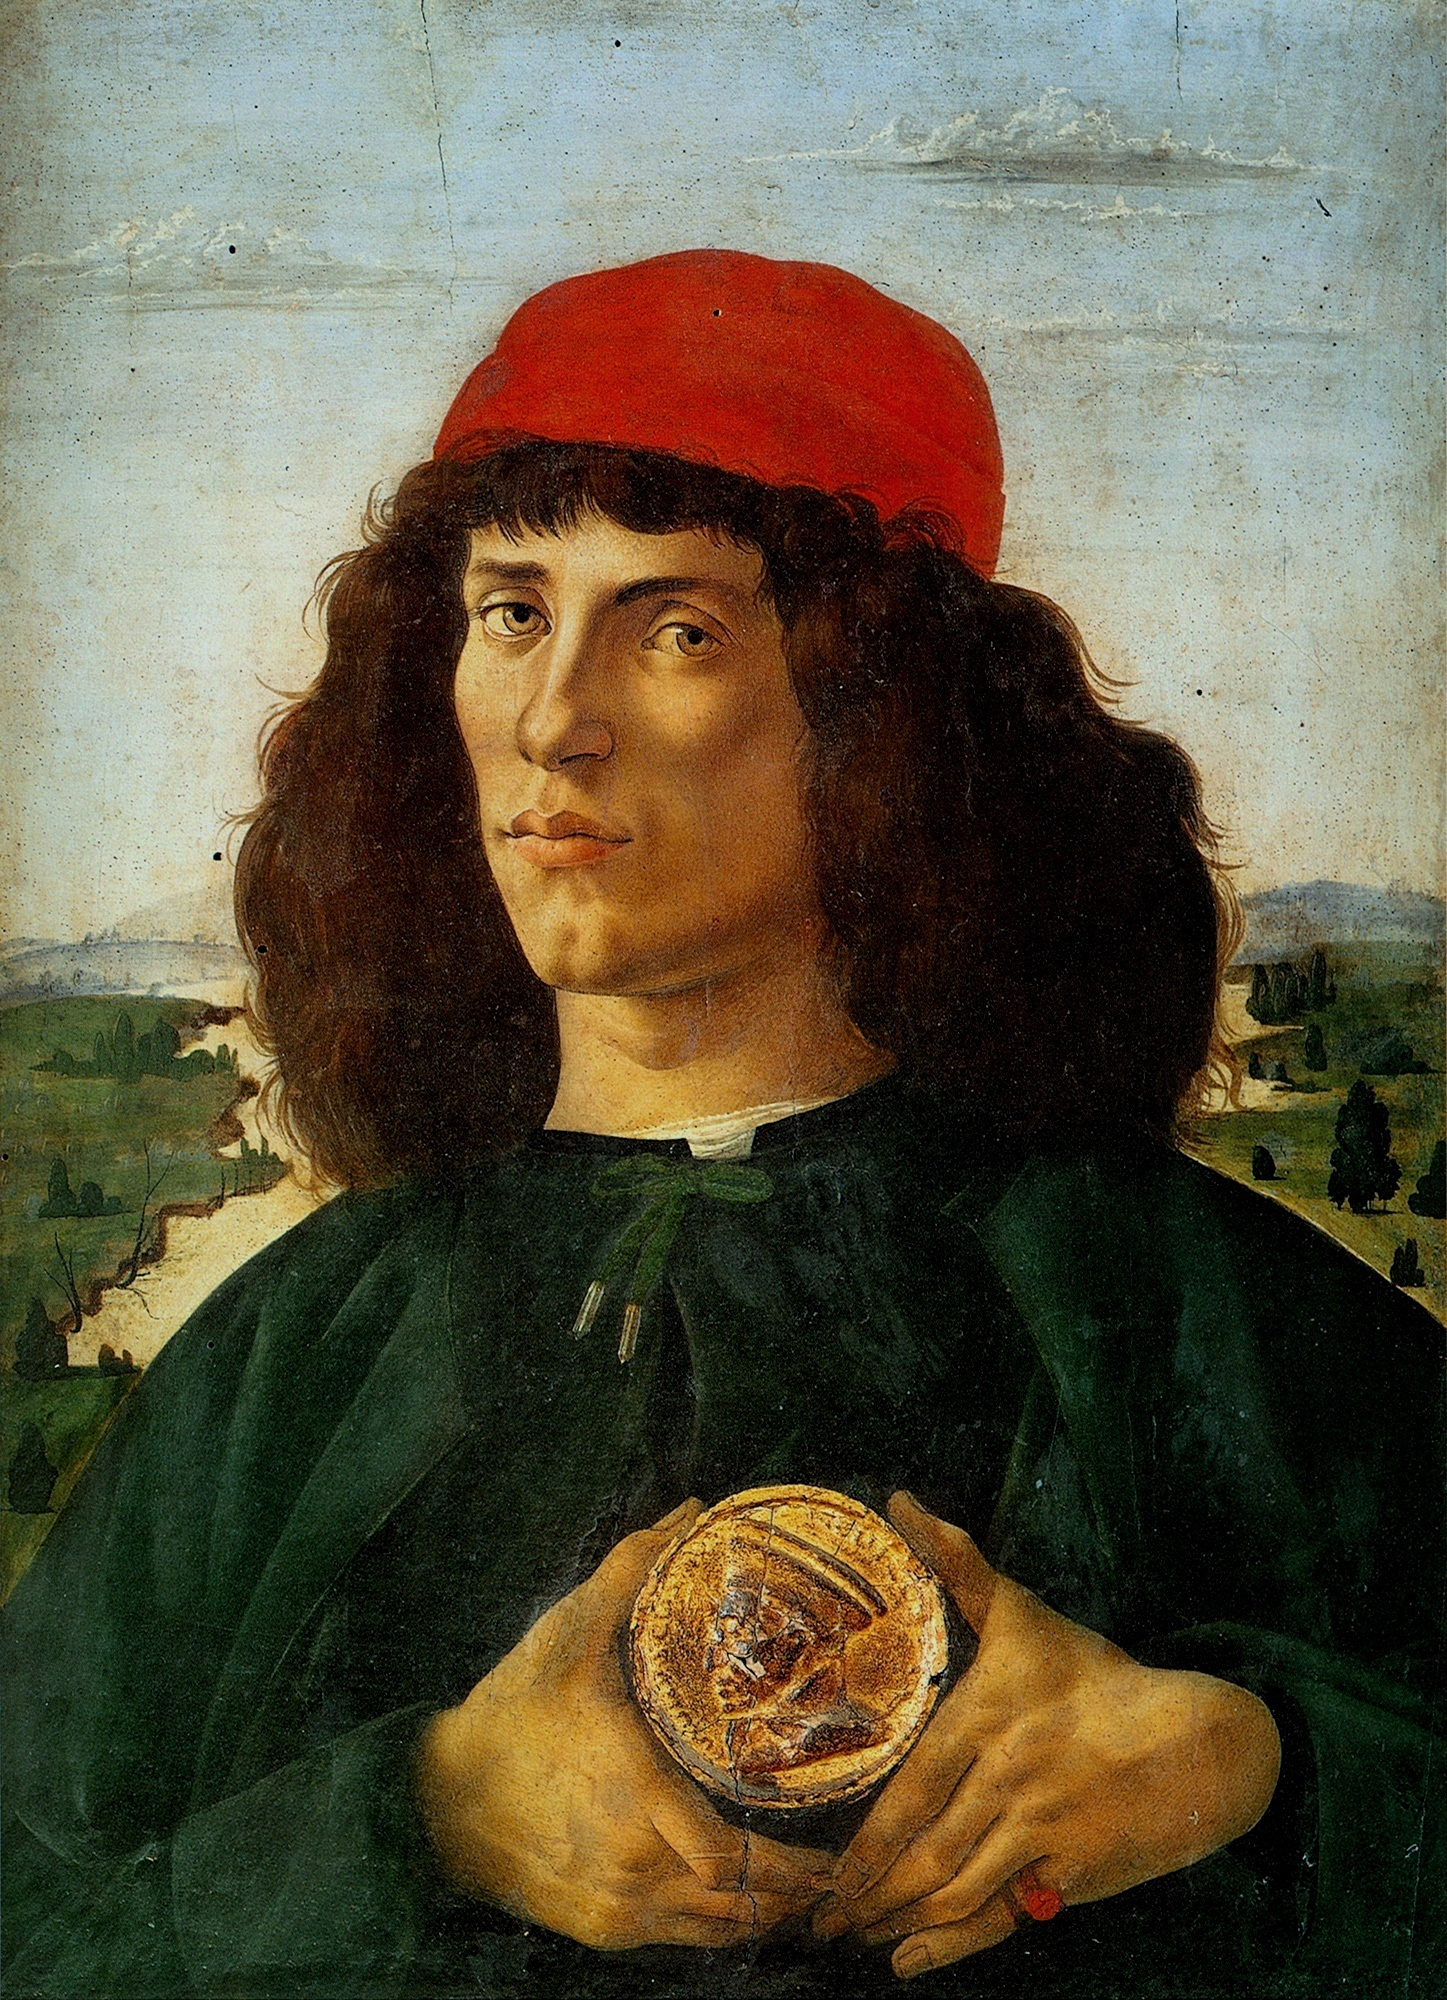
\includegraphics[width=\textwidth,height=0.75\textheight,keepaspectratio]{imgs/botticelli.jpg}
\caption{Botticelli's \emph{Portrait of a Man with a Medal of Cosimo the Elder}}
\label{botticelli}
\end{figure}

The second innovation was the organisational structure of the Medici Bank. The Medici used a different organisational structure than was typically seen in Florence during this time. Traditionally we would see centralised and hierarchical banking houses--like the Alberti bank. Due to the banks initial roots in Rome it quickly established a branch-based system in both Rome and Florence. Subsequently, the bank designed an organisational structure that was more decentralised and governed by a set of harmonised lending rules within all of its branches. This decentralised network allowed for the diversification of loans and ultimately the reduction of risk, which lowered the cost of banking. Their organisation reflected that of a joint stock company whereby the parent company, located in Rome, controlled the subsidiary partnerships by owning more than 50\% of the capital of its branches. Other partners also owned substantial amounts of stock within the subsidiary banks meaning that their compensation was tied in with the banks performance.

Instead of a salary branch managers were junior partners who received a share in the profits plus an allowance for living expenses. The system provided incentives for increasing effort levels and lowering risk-shifting. Moreover, a promotion system and hierarchy was obvious in that a satisfactory manager had a high chance of becoming a partner and thereby greatly increasing his earnings. The Medici did not have the power to dismiss the junior partners, but rather had the power to condemn partners at any time. In effect, the Medici Bank had created an organisational architecture similar to that of a limited liability holding company. Under this structure decision-making was decentralised and the risk burdened on the Medici was diluted by being differentiated across the activities of other branches. Moreover, the structure gave the Medici themselves easy oversight, a clear locus of control and therefore the ability to create rule sets that had to be accepted by the other branches.

It could be argued that the Medici's organisational structure evolved to adapt to transaction costs that were prevalent within the firm. Decision rights were decentralised throughout the organisation to make use of local information but, as a consequence, partners could be opportunistic with their resources and abilities. In particular, partners could damage the Medici's reputation and profitability through risk-shifting or through privately capturing the gains from lending activities. Partners within the organisation require monitoring and evaluation from central authorities; however monitoring and the transfer of information from Rome to Florence would be costly. The costs of monitoring partners were reduced through the incentive alignment that comes with providing partners from different branches stock in their branch. Decision management and control responsibilities become attached to the residual claimants of the firm.

\subsubsection{Social structure of the political and economic elite}

The theoretical perception of the entrepreneur developed above highlights the importance of the positional attributes of economic agents for the exploitation of power and influencing change. Although the process and organisational innovations were pioneered by Giovanni, the positional power of the Medici within the Florentine elite can be attributed mainly to Cosimo as a political networker. After laying the foundations, Giovanni stepped down from the bank due to illness and ownership transferred to Cosimo, Giovanni's son, who led the Medici family to political dominance. Cosimo consolidated political and economic power in an entrepreneurial manner by leveraging a central position in the networks of elite family inter-marriages, economic relationships and political patronage. 

Cosimo's success was not specifically due to his superior business leadership, but rather to his superior networking ability and patronage of the arts which became of increasing importance as the Renaissance began to flourish. He was therefore multiply embedded in various aspects of the socio-economic space, playing a role in complex and overlapping Florentine marriage, economic, and elite political patronage networks. He was riding herd on vast macro-political and macroeconomic forces far beyond his control. Yet he founded a political dynasty that dominated Florence for over three centuries. He consolidated a Europe-wide banking network that helped induce both international trade and state making elsewhere. And he oversaw and sponsored the Florentine intellectual and artistic effervescence that we now call the `Renaissance'. Such sprawling success of a single individual is largely due to two factors: the economic success of the Medici Bank and Cosimo's positional power within the socio-economic networks present in Florence at the time.

We defined multivocality as corresponding to an agent who specialises in a number of different roles and therefore may directly operate in a number of different aspects of a socio-economic space. We use this definition of multivocality with an application to Cosimo de'Medici to explain the prominence of his position in the socio-economic space. To do this we must first note that the Medici benefitted from the restructuring of the marriage networks which occurred over the decades following the Ciompi Revolt and subsequent counter-revolution. Marriage networks were strategically restructured in order to segregate those who sympathised with the Ciompi and those who did not: intra-elite marriages were conceived partially in political alliance terms and were used to strengthen the elite's position such that further revolutions by coalitions of workers could not emerge again. The elite families that did not sympathise with the Ciompi tended to marry with other non-sympathisers. This resulted in a tight-knit marriage network of socio-economic equals within their oligarchic neighbourhoods. Conversely, sympathisers called the ``New Men'', did not tend to marry into other sympathising families--each elite family remained relatively isolated.

\begin{figure}[h!]
\centering
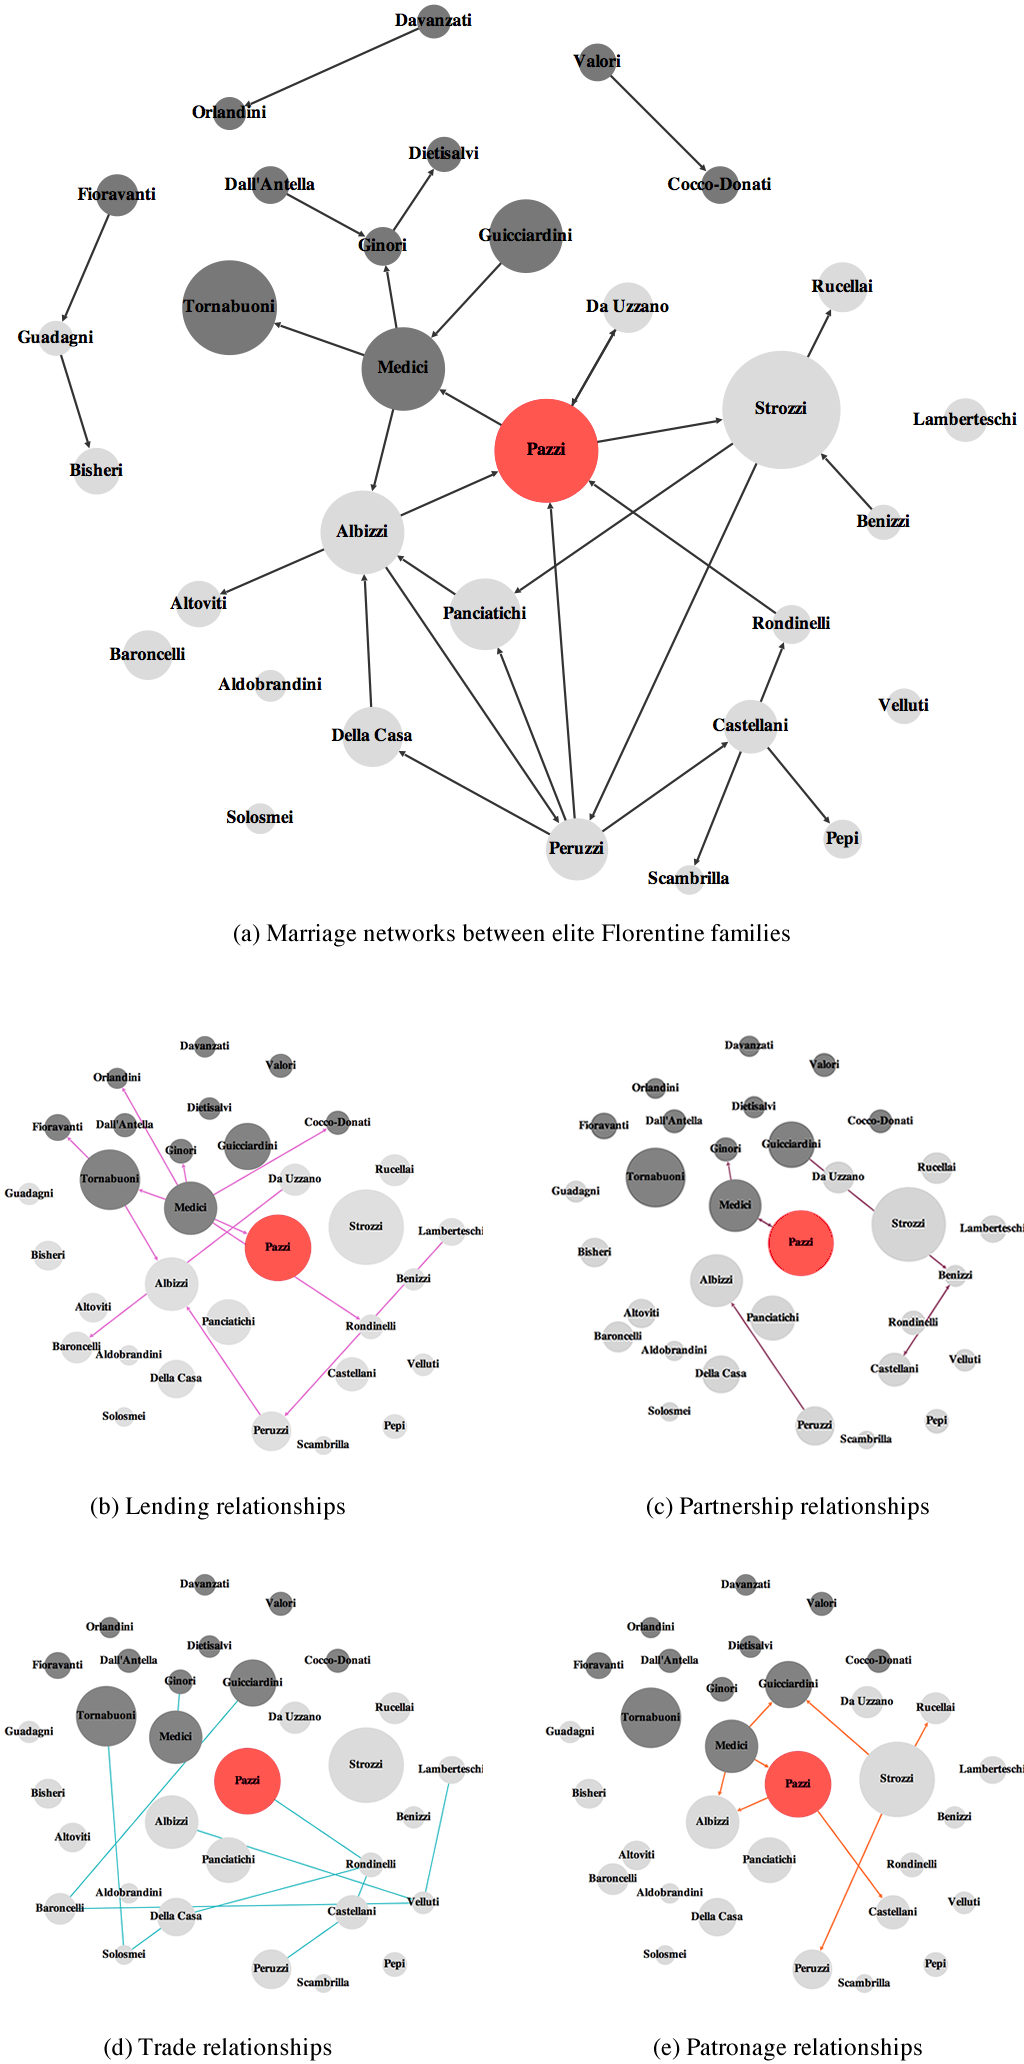
\includegraphics[width=\textwidth,height=0.9\textheight,keepaspectratio]{imgs/allnetworks.png}
\caption[Social and economic relationships between elite Florentine families]{Five network diagrams highlighting social and economic relationships that existed between elite Florentine families circa 1429.}
\label{florentinenets}
\end{figure}

The Medici's neutral stance during the period immediately after the Ciompi Revolt--as well as their aforementioned business and social success due to Giovanni's innovations--made them attractive to both sides of the oligarchic elite. Over time the Medici, both strategically and fortuitously married into both sides and the resulting position in the social network allowed the Medici family to build and control an early forerunner to a political party, while the other elite families of the time suffered from internal power-struggles. It must be reminded to the reader that all of the elite marriages recorded here were strategically arranged by patriarchs or their equivalents in the two families. As \citet[p.~1259]{Padgett1993} describe it, ``[the] Medician political control was produced by network disjunctures within the elite, which the Medici alone spanned''. Such a claim is evident with the aid of the set of graphs in Figure \ref{florentinenets}. This Figure provides five networks on the same set of families. Each network concentrates on a certain type of relationship. Specifically, network (a) shows marriage relationships that were strategically formed between families, network (b) shows the lending relationships between the families, network (c) shows partnership relationships, network (d) shows bilateral trade relationships between these families, and network (e) shows patronage relationships. The marriage network, the loan network, and the patronage network all indicate that the Medici filled a structural hole between the two opposing sides in both a social and an economic sense. Cosimo created a new and unique socio-economic role through his network position; a de facto ``president'' of Florence who, although never occupied office, had complete control of the political and therefore the institutional and economic environment of Florence and Northern Italy.

There are two interesting points to note with regard to the above marriage network. The first point highlights the importance of the composition of both marriage and economic linkages within the families in Florence. Each family's respective actions depended not only on independent rationalised decision-making, but also on how they are interlinked. It can be seen that power and influence reverberated through the marriage linkages meaning that the very composition of the marriage network within these families matters. When considering the ``New Man'' revolution of 1429, when the ostracised traitors rebelled against the oligarchic elite, it became apparent that the dense structural interconnectivity of the oligarchic elite rendered them highly disorganised as control was decentralised through the marriage network. Power struggles emerged with so many intertwined socio-economic equals. The collective-action problem remained as they failed to realise a focal point in the form of a leader who could strategise and initiate action. The composition of their network thus affected their cohesiveness in times of crisis; each family schemed with other families to which they were tied as to the best course of action. Opposing stratagems arose between the different inter-linked families, ultimately generating tensions between the ruling elites as opposed to the necessary robust action. In effect, they became bound by their own network. Social ties can provide constraints as well as opportunities when individuals pursue their own self-interest without any clear governing rule-sets or leaders.

Whilst the oligarchs hesitated, the Medici was able to solve their collective action problem and mobilise their party. This was largely because of the composition of the marriage network underlying the party which centralised around the Medici. Indeed, the Medici were married into three other families directly, the Tornabuoni, the Ginori and the Guicciardini; this was combined with the fact that the other member families were not heavily interlinked through marriage as was witnessed with the oligarchic partisans. This provided a focal point which allowed for collective action. Such a situation provides an empirical basis in which to appreciate the power-dependence literature \footnote{For a seminal discussion on this literature see \citet{Emerson1962}}. It is easy to appreciate how the dependence on a powerful and respectable family would be needed for collective action.

The second point highlights the entrepreneurial characteristic which brought the Medici family and Cosimo to power. The characteristic specifically refers to the Medici's centralised position within the social network of the ruling elite. As seen above, the Medici family developed a star network which spanned both the oligarchic partisans and the Ciompi sympathisers. Such a position meant that followers of the Medici could only interact with the rest of the followers through mediation of the Medici. Moreover, if they wished to discuss issues with the oligarchic rulers, all information had to pass through the Medici and vice versa. From their strategic position in the social network they were able to remain in power as brokers of important information. To signify the powerful role of the Medici Pope Pius II claimed: "Political questions are settled in his [Cosimo's] house. The man he chooses holds office... He it is who decides peace and war and controls the laws... He is King in everything but name" \citep{Hibbert1980}.

\subsection{The interaction of networks, institutions, and entrepreneurs}

Henrekson \& Sanandaji highlight the interaction between political and market entrepreneurship. In doing so they explain how the economic and political spheres of the socio-economic space can interact with each other and facilitate development. Particular attention is paid to how institutional entrepreneurs can affect the rules of the game and therefore the relative payoffs to, and allocation of, entrepreneurial activity within the economy. This interdependent development is illustrated by the authors specifically with the example of Silvio Berlusconi, who used his economic power from market activities to fuel his political dominance in Italy. His media empire throughout Italy provided him a platform to advertise himself, distribute his policies and influence the beliefs of the voting citizens of Italy. The outcome of Berlusconi's efforts can be labelled as unproductive and potentially destructive to society's welfare: indeed, there is evidence to show that throughout his business career he has used his political ties to seek and capture rents. Through market innovation the actions of entrepreneurs can influence a change to the institutional setting of the economy: this can be a consequence of direct or indirect effects. The interaction between market and political spheres of the socio-economic space is also notable with respect to the success of the Medici family. Furthermore, although not discussed by Henrekson \& Sanandaji, we suggest that the positional attributes of individual agents impact their power to influence the institutional environment of the socio-economic space. This is particularly apparent with the aforementioned network regarding the Florentine elite and the theory of relational entrepreneurship: Cosimo and the House of Medici influenced institutional change and the actions of elite Florentine factions primarily due to their positional attributes, which was formed as a consequence of their market entrepreneurship.

The above perspective of relational entrepreneurship extended the insights of Henrekson \& Sanandaji, noting that the position of an individual agent within a networked socio-economic space can inform their ability to broker information and exchange, and thus potentially gain a powerful position within a network. As such, entrepreneurial agents can form and exploit unique positions within a network, which can subsequently have an institutional impact. The unique position attained by economic agents, as discussed throughout the dissertation, can emerge as a consequence of the development of new socio-economic roles. As such, the relational perspective provides a way to investigate the interaction between these three important elements: institutions, socio-economic networks, and entrepreneurship. The interacting elements of institutions, socio-economic networks, and entrepreneurship can be easily applied to the case of the Medici as discussed thus far.

% \section{Concluding points and future discussions on socially structured economies}

    % Add some concluding points

    % Introduce the next Part
\part{Entrepreneurship in a Platonian Economy} 
\label{part:entrepreneurshipPlatonianEconomy}

\section*{Overview of Part II}

When discussing the representative states of the socio-economic space we defined the Platonian economy as an organic state within which the generation of wealth derives from social organisation founded on the horizontal division of labour. There does not exist hierarchical production organisations, firms, or platforms that generate economic wealth. Instead, wealth is generated through the interaction of specialised consumer-producers within a network of mutually beneficial bilateral exchanges. Economic agents are assumed to be equal within the trade such that there exists no exercise of authority within the exchange. The Platonian economy is, in a sense, the most simplistic social economy: there exists a juvenile, yet non-trivial, governance system and a set of economic interactions between individual consumer-producers, but no social organisation beyond this point. As a result the number of socio-economic roles are limited, the interaction inefficiency between agents is assumed to be large, and role-building costs are large.

Part~\ref{part:entrepreneurshipPlatonianEconomy} focuses on economic interaction and entrepreneurship within a Platonian socio-economic space. To do so we build on materials developed in Chapters~\ref{ch:relationalperspective},~\ref{ch:relationaltheory}, and~\ref {ch:entrepreneurship}. Focus is placed on the interaction between entrepreneurs, the development of new socio-economic roles, and the impact that entrepreneurship has on the interaction infrastructure of the socio-economic space and the positional attributes of individual consumer-producers. Lemma~\ref{con:positionalattributes}, as well as the discussion in the previous chapter plays an important role throughout. Above, we noted that an entrepreneur can manipulate different layers of the socio-economic space: focus here is on identifying a relationship between entrepreneurship, unique relational positions of entrepreneurial agents within an interaction infrastructure, and how entrepreneurs attain and exploit power within a Platonian economy.

\subsection*{Chapter breakdown}

To express unique positions and power within a networked interaction infrastructure we extend the mathematical definition of the socio-economic space to include network theory as initially discussed in Section~\ref{sec:socialeconomicnetworks}. Chapter~\ref{ch:criticalnodes}, \emph{Middlemen as entrepreneurs}, introduces these theoretical network concepts as well as a set of metrics to measure the positional power of economic agents within a Platonian socio-economic space. The metrics are defined over critical nodes; which we claim represent entrepreneurs that have developed a unique socio-economic role and thus position within the interaction infrastructure. These metrics are applied to the empirical application of the elite Florentine families introduced in Section~\ref{ex:houseofMedici}.

Chapter~\ref{ch:blocks}, \emph{The formation of extractive structures in networks}, directly extends the notions discussed in Chapter~\ref{ch:criticalnodes} to multiple economic agents and thus sets of nodes. Non-cooperative game theory the main methodological tool used to assess the individualistic cooperation of economic agents within a networked environment. An important aspect of entrepreneurship is the alteration of the interaction infrastructure of the socio-economic space. The formation of `blocks' within an interaction infrastructure is a direct representation of network-oriented entrepreneurial action; the outcome of which is the formation of new socio-economic roles. Furthermore, this form of entrepreneurial action can be viewed in terms of merger, cartel, and acquisition activity.
\chapter{Middlemen as entrepreneurs}
\label{ch:criticalnodes}

Research has recognised networks as important descriptors of social and economic processes \citep{Watts2004,Jackson2008,Newman2010}. The outcome of the agent-based simulations in Chapter~\ref{ch:relationaltheory} showed that as the networked interaction infrastructure develops the set of economic interactions and relationships can form an irregular topology where individual agents hold heterogeneous positions in the infrastructure. As a consequence of their interactions some economic agents hold more `central' positions in the infrastructure than others: the centrality of individual economic agents is distributed unevenly across the network. We noted in the previous chapter that the formation of a new socio-economic role through entrepreneurial effort comes with it the formation of a unique set of economic interactions and thus a unique position in the socio-economic space. The unique position of individual agents is closely related to the discussion of the middleman here.

This chapter makes a contribution to the analysis of economic agents, depicted generally as nodes, that are critical for the flow of information and trade in a network. Such critical agents---or ``middlemen''---have been solely considered for undirected networks. Here, we consider these nodes in the more general context of directed networks. We introduce a middleman as a specific type of node that can block the information flow from at least one node to another. If one applies this definition to undirected networks, one arrives at the standard notion of a middleman as a singleton node cut set. In the context of directed networks this is no longer the case: Its removal does not necessarily break up the whole network; it just compromises the information flow for at least one pair of nodes. In networked economies, the essential brokerage position of middlemen allows them to be highly extractive to both directly and indirectly connected nodes. On the other hand, their involvement lowers transaction costs in terms of search and the formation of beneficial links \citep{Burt1992}.

Naturally, the existence of middlemen is closely related to the competitive environment represented by that network. \citet{GillesDiamantaris2013} show in a very simple setting that middlemen have the potential to be highly exploitive given a lack of competition combined with a pessimistic outlook regarding their potential contestability in a network. The main conclusion from this research is a non-trivial extension of how economists and social scientists perceive the architecture and dynamics of exchange systems, how the presence of a middleman can knit a system together, and, as a consequence of their position, can act as rent-extracting monopolists with excessive bargaining power \citep[Chapter~11]{EasleyKleinberg2010}.

We extend these notions to a more general definition of contestability in directed networks. In a directed network, a node is contested if alternative pathways are available to establish exchange between pairs of nodes in the network. Our main result shows that there is a formal duality between the existence of middlemen and network contestability. In particular, an intermediary node is a middleman if and only if it is uncontested.

One would expect that betweenness centrality measures would capture the influence that such middlemen exert. However, we show that this is not the case. Instead, we propose a new \emph{middleman power measure} that exhibits the desired properties. We devise an algorithm that applies the adjacency matrix of any directed network to identify and measure the middlemen in that network. We apply this algorithm to study two very well known (historical) directed networks from the literature. These applications allow us to make an in-depth comparison with well-established centrality measures such as betweenness centrality and Bonacich centrality \citep{Bonacich1987}.

In the Florentine marriage network of the early renaissance \citep{Padgett1993,Padgett1994}, we conclude that our middleman power measure clearly ranks the more powerful middlemen higher than the less powerful, confirming with historical analysis. In \citet{Krackhardt1987}'s advice network, again our measure confirms Krackhardt's original assessment of the most influential node. Furthermore, we show that, despite the importance of middlemen in these networks, this positional feature is not properly and fully identified by conventional centrality measures.

\paragraph{Middlemen as entrepreneurs.}

In complementing our claim regarding the relationship between middlemen and competition, we consider middlemen as entrepreneurs. Middlemen are regarded as economic agents that form a new socio-economic role and therefore possess a unique position within society; they connect to otherwise disconnected agents and gain from the bridging of communities and the integration of ideas and specialisations.

We note that the economic state of the Platonian economy is used throughout the assessment of the next two chapters; and as such we concentrate on the existence of a horizontal division of labour\footnote{However, some easy extension can be made to capture phenomena in more vertical divisions of labour.}. The horizontal division of labour allows for the production of relatively complex consumption goods, which are only realised through a sequence of intermediate stages performed by distinct individuals. This is exactly what is depicted throughout this chapter as we consider such concepts as \emph{contestability} in networks. From the flow of exchange through intermediation, some economic agents may be considered as more powerful and influential than other agents. \emph{Node centrality} can help to identify the most influential economic agents in the socio-economic space.

\subsubsection{Standard measures of node centrality}

Middlemen have been investigated in both sociology and economics during the past three decades. The specific interest in economics was initiated by \citet{KalaiMiddlemen1978} who investigated the payoffs to middlemen in an intermediated trade environment. These insights were extended by \citet{RubinsteinWolinsky1987} who applied them to a model of market search. \citet{JacksonWolinsky1996} and \citet{GillesChakrabarti2006} further analysed middlemen in the context of economic interaction.

Many of the general findings in the economics literature have been independently verified in the social sciences. In social network analysis, middlemen are seen as social actors that bridge structural holes in the social fabric. Due to their position these middlemen have access to more diverse information; are able to broker information and ideas between agents and affiliations; will have a tendency to be more entrepreneurial; are able to exploit their intermediating opportunities; and have better ideas which are then evaluated by others within a society or organisation \citep{Burt1992, Burt2004,Burt2005,Burt2010}. Moreover, by virtue of their weak ties in the network, middlemen are able to exploit unique opportunities that are not afforded to other, more socially embedded, nodes in the network \citep{Granovetter1973, Granovetter2005}.

Despite the wide acknowledgement within social network analysis of the significance of middlemen, centrality measures do not necessarily identify these critical nodes as being important even though their removal may deteriorate the functionality of the network as a whole. As the notion of centrality came to the fore, \citet[p.~219]{Freeman1979} argued that central nodes were those ``in the thick of things''. To exemplify this, he used an undirected star network consisting of five nodes. The middle node, at the centre of the star, has three advantages over the other nodes: It has more ties; it can reach all the others more quickly; and it controls the flow between the others. Freeman developed three simple measures of node centrality based on the prevalent features of the center node: degree, closeness and betweenness.

More complex centrality measures have been proposed. \citet{Bonacich1972,Bonacich1987,Bonacich2001} proposed the use of the largest eigenvalue of the adjacency matrix as the basis for the measurement of network centrality. This measure expresses the idea that a node is more central if it is connected to nodes that are themselves central. Other measures, including Katz centrality \citep{Katz1953} take advantage of the same mechanism as Bonacich centrality by analysing the number of all nodes that a given node can be connected through a path, while contributions from linking distant nodes are progressively penalised. A node has a larger centrality if it has neighbours with a high Katz centrality. PageRank \citep{BrinPage1998} is a variant of Katz centrality, which recently gained application to the World Wide Web. Moreover, these common measures of centrality have been applied to many different social and economic contexts, and have had application to directorate networks (Khanna et al., 2015; El-Khatib, 2015).

The most common centrality measures do not provide a proper account of network power and, usually, overlook middlemen. Two exceptions are noted: First, the $\beta$-measure \citep{BrinkGilles1996, BrinkGilles2000} is founded on an axiomatic approach to measuring centrality. This measure is one of a few that measures dominance, and therefore power, in directed networks. \citet{BormBrink2002} develop an iterated $\beta$-measure which, much like the eigenvector and PageRank centralities, develops a score based on the dominance of the nodes that it dominates. Again, this lacks a specific application to directorate networks. Applications are mainly focussed on how nodes are dominated by others in hierarchical organisations. Second, \citet{Bozzo2015} provide both a vulnerability and power measure based on the number of nodes that can be victimised by so-called ``executioners''. The power of a node set is comparable to how integral the set is to the robustness of an undirected network.

\paragraph{Chapter outline.}

This chapter is partitioned into four sections. The first provides the required preliminaries for our analysis and introduces strong and weak middlemen within networked socio-economic spaces. We also consider the notion of network contestability, which is shown to be the dual notion to that of middlemen. The second section discusses a measure of middleman power, which assigns a quantitative expression to a node's brokerage power. The third section provides a variety of measures in which to assess the competitiveness of a network in both a static and dynamic sense. The final section investigates two empirical case studies of social networks where middlemen have tended to have importance: the Florentine marriage network and Krackhardt's advice network.

\section{Middlemen and contestability}

Our initial discussion focuses on the definition of a critical nodes in a directed network, which we denote as \emph{middlemen}. We introduce middlemen in relation to the connectivity in a network. In doing so we identify two related notions of middlemen, denoted as strong and weak middlemen depending on their network position.

\subsection{Preliminaries}

We formally defined a socio-economic space as a set of economic interactions between a population of consumer-producers or economic agents, the result of which forms a network of relations. This definition infers that all social and economic interaction is two-way and thus symmetric. In reality, not all interactions and relationships are bilateral; especially when considering the flow of intermediate goods or information in a network. This distinction between symmetric and asymmetric relationships can be represented by undirected and directed relationships.

\paragraph{Directed and undirected networks.}

The network that is described through the formal definition of a socio-economic space is considered as an \emph{undirected network} such that all interactions are symmetrical. For example, given an undirected relationship between two agents, both agents can interact with each other. Many fundamental social and economic engagements can be considered in this symmetric manner.

A more generalised version of an undirected network is a \emph{directed network} which consists of directed relationships. A directed relationship between two agents is considered asymmetric such that one agent can interact with the other, but this interaction is not reciprocated. We note that a directed relationship is more general than an undirected relationship because a reciprocated directed relationship leads to an undirected relationship. Directed relationships and networks are also useful to describe social and economic networks. Specifically they can be used to describe the flow of information and economic goods and commodities within social and economic relationships.

We analyse social and economic interactions in terms of a set of directed relationships that forms a directed network. A directed network is a pair $(N,D)$ where $N = \{1,2, \ldots ,n\}$ is a finite set of economic agents, or \emph{nodes}, and $D \subset \{ (i,j) \mid i,j \in N$ and $i \neq j \}$ is a set of \emph{arcs}, being directed relationships from one node to another. Note that $(i,i) \notin D$ for any $i \in N$, which is a technical requirement\footnote{An \emph{undirected} network can be interpreted as a directed network $(N,D)$ such that all arcs are reciprocated: $(i,j) \in D$ if and only if $(j,i) \in D$.}. We denote a directed network $(N,D)$ by $D$ unless $N$ is ambiguous. Also, we denote $(i,j) \in D$ by $ij$. We next introduce some auxiliary concepts in directed networks.

\paragraph{Walks.}

A \textit{walk} from $i$ to $j$ in a directed network $D$---or, simply, a $(i,j)$-\emph{walk}---is a set of connected nodes $W_{ij} (D) = \{ i_{1}, \ldots ,i_{m} \} \subset N$ with $m \geqslant 3$, $i_1 =i$, $i_m =j$, and $i_{k}i_{k+1} \in D$ for every $k=1, \ldots ,m-1$. Therefore, a walk is a sequence of adjacent nodes in the network. Walks might revisit nodes and, therefore, might contain loops.

In many cases there are multiple walks from $i$ to $j$ in a directed network $D$. If this is required, we denote $W_{ij}^{v}(D)$ as the $v^{\mbox{th}}$ distinct walk from $i$ to $j$ in $D$.

The class $\mathcal{W}_{ij}(D)= \{ W_{ij}^{1}(D), \ldots ,W_{ij}^{V}(D) \}$ consists of all distinct walks from $i$ to $j$ in $D$, where $V$ is the number of distinct walks. $\mathcal{W}_{ij}(D)= \varnothing$ denotes that there is no walk from $i$ to $j$ in $D$.

\paragraph{Connectedness.}

Nodes $i,j \in N$ are \textit{strongly connected} if $\mathcal{W}_{ij}(D) \neq \varnothing$ as well as $\mathcal{W}_{ji}(D) \neq \varnothing$. A directed network $D$ is \emph{strongly connected} if $\mathcal{W}_{ij} \neq \varnothing$ and $\mathcal{W}_{ji} \neq \varnothing$ for all nodes $i,j \in N$.

Node $i$ is \textit{weakly connected to} $j$ if $\mathcal{W}_{ij}(D) \neq \varnothing$. A directed network $D$ is weakly connected if for all $i,j \in N$ either $i$ is weakly connected to $j$, or $j$ is weakly connected to $i$, or both. Clearly, strongly connected networks are always weakly connected.

A subset $M \subset N$ is a \emph{weakly connected component} of $D$ if $(M, D_M)$ with $D_M = D \cap (M \times M)$ is weakly connected and and there is no $i \in N \setminus M$ with $(M+i, D_{M+i})$ being weakly connected.

\paragraph{Successors and predecessors.}

If $\mathcal{W}_{ij} (D) \neq \varnothing$ then $j$ is called the \textit{successor} of $i$ and $i$ is called the \textit{predecessor} of $j$ in $D$.

For $i \in N$ we define $s_{i}(D) = \{ j \in N \mid (i,j) \in D \}$ being all of the \textit{direct successors} of $i$ in $D$, and $p_{i}(D)=\{j \in N \mid (j,i) \in D\}$ being all the \textit{direct predecessors} of $i$ in $D$. The \emph{out-degree} of $i$ is given by $d_{i}^{+} = \# s_{i}(D)$ and its \emph{in-degree} by $d_{i}^{-}= \# p_{i}(D)$. Now, $i$'s overall degree is given by $d_{i} = \# \{ s_{i} (D) \cup p_{i} (D) \}$.

We also use $P_{i}(D)=\{j \in N \mid \mathcal{W}_{ji}(D) \neq \varnothing \}$ which denotes $i$'s \textit{predecessor set}, and $S_{i}(D)= \{j \in N \mid \mathcal{W}_{ij}(D) \neq \varnothing \}$ being $i$'s \textit{successor set}\footnote{We emphasise that we do not include $i$ in its own predecessor or successor set.}. Node $k$ is an \emph{indirect successor} of $i$ in $D$ if $k \in S_{i}(D) \setminus s_i (D)$ meaning that $\mathcal{W}_{i,k}(D) \neq \varnothing$. Thus, $i$'s successor set includes all of $i$'s direct and indirect successors.

Likewise, node $k$ is an \emph{indirect predecessor} of $i$ in $D$ if $k \in P_{i}(D) \setminus p_{i}(D)$, i.e., $\mathcal{W}_{k,i}(D) \neq \varnothing$. $i$'s predecessor set consists of all of $i$'s direct and indirect predecessors.

\begin{definition}[Origin and reach] \label{coverage}
Consider a directed network $(N,D)$ and a node $i \in N$.
\begin{itemize}
\item The \textbf{origin} of node $i$ denotes the fill set of $i$'s predecessors including node $i$
\begin{equation}
\overline{P}_{i}(D) = P_{i}(D) \cup \{i\}.
\end{equation}
\item The \textbf{reach} of node $i$ denotes the fill set of $i$'s successors including node $i$
\begin{equation}
\overline{S}_{i}(D) = S_{i}(D) \cup \{i\}.
\end{equation}
\end{itemize}
\end{definition}

The node set $N$ can be partitioned into three disjoint subsets: sources, sinks, and intermediaries. Node $i$ is a \emph{source} if $d_{i}^{-} = 0$ and $d_{i}^{+} \geqslant 1$; $i$ is a \emph{sink} if $d_{i}^{-} \geqslant 1$ and $d_{i}^{+} = 0$; and $i$ in an \emph{intermediary} if $d_{i}^{-} \geqslant 1$ and $d_{i}^{+} \geqslant 1$.

Finally, we let $i \in N$ and $D-i$ be equivalent to:
\begin{equation}
D - i = D_{N \setminus i} = \left\{ (j,h) \in D \mid j,h \in N \setminus i \right\} .
\end{equation}

Therefore $D_{N \setminus i}$ is the restricted network that removes all nodes in node set $i$ and all arcs to and from the nodes in $i$.

\subsection{Connectivity and middlemen}

We identify \textit{critical nodes} as those having the ability to broker information flows in a network. Following \citet{GillesChakrabarti2006}, a critical node in an undirected network can disrupt and manipulate the typical operations on a network by disconnecting two or more nodes---which is equivalent to the property that removing a critical node partitions a given network into multiple disconnected components.

Here, we extend this concept to directed networks. In this context our definition focusses on the disruption of connectivity of two nodes.

\begin{definition}[Middleman] \label{middleman}
Let $D$ be a network on node set $N$, where $h \in N$.
\begin{itemize}
\item Node $h$ is an \textbf{$(i,j)$--middleman} if for some pair $i,j \in N$ $\mathcal{W}_{ij} (D) \neq \varnothing$ and
\begin{equation} \label{ijmiddleman}
h \in \bigcap \mathcal{W}_{ij}(D) \setminus \{i,j\} = W_{ij}^{1}(D) \cap  \ldots  \cap W_{ij}^{V}(D) \setminus \{i,j\},
\end{equation}
where $V \geqslant 1$ is the number of walks from $i$ to $j$. Here, $M_{i,j}(D) \equiv \cap \mathcal{W}_{ij}(D)$ denotes the \textbf{$(i,j)$--middleman set} containing all $(i,j)$--middlemen.

\item The \textbf{middleman set} for $D$ is the set of all middlemen in $D$ given by
\begin{equation} \label{middlemanseteq}
M(D) = \bigcup_{i,j \in N \colon i \neq j} M_{i,j}(D)
\end{equation}
Node $h$ is a \textbf{middleman} if $h \in M(D)$ and $h$ is a \textbf{non-middleman} if $h \notin M(D)$.
\end{itemize}
\end{definition}

A middleman is an intermediary node that is a member of \emph{all} walks between at least two other nodes within a given network. Therefore, a middleman brokers the flow of all information between at least two nodes. Obviously, a middleman connects two or more agents that would not be connected otherwise. Indeed, by definition $M_{i,j} (D) \neq \varnothing$ if and only if $\mathcal{W}_{ij} (D) \neq \varnothing$.

Converse to a middleman, a non-middleman is an intermediary that if removed from the network does not affect the connectivity of any two or more other nodes and, therefore, does not impose a negative externality on other nodes when removed.

The following properties can be deduced directly from the above definition.

\begin{proposition}\label{TheoremIntermediary}
Let $D$ be a directed network on the node set $N = \{ 1, \ldots ,n \}$.
\begin{numm}
\item Every middleman $i \in M(D)$ is an intermediary in $D$. 

\item If $n < 3$, there might exist intermediaries, but there are no middlemen.

\item For $n \geqslant 3$ and $i \in N$, $p_{i}(D) \subset \left[ p_{j}(D) \cup \{ j \} \, \right]$ for every direct successor $j \in s_{i}(D)$ implies that $i \notin M(D)$.

\item For all $i,j \in N$ with $j \in s_{i}(D)$ it holds that $M_{i,j}(D) = \varnothing$.
\\
This implies that the complete directed network has no middlemen.

\item Every middleman $i \in M(D)$ has a local clustering co-efficient of less than $1$.

\item If $D$ is undirected in the sense that $(i,j) \in D$ if and only if $(j,i) \in D$, then $M_{ij} (D) = M_{ji} (D)$ for all $i,j \in N$.
\end{numm}
\end{proposition}

From (vi), in an undirected network a node is a middleman if it rests on all walks from node $i$ to node $j$. This means that the removal of a middleman disrupts the any communication between nodes $j$ and $i$. Hence, a middleman indeed is a singleton cut set in an undirected network, as traditionally understood.

On the other hand, in a directed network, a middleman rests on all walks from node $i$ to node $j$, but does not have to rest on all walks from $j$ to $i$. This implies that given the removal of a middleman in a directed network the interaction from $i$ to $j$ will become disconnected, but the interaction from node $j$ to node $i$ may still be present. Indeed, even with the removal of a middleman in a directed network, nodes $i$ and $j$ can still remain weakly connected. This insight motivates a further refinement of the notion of a middleman in a directed network.

\begin{definition}[Strong and weak middlemen] \label{strongweakmiddlemen}
Let $D$ be a weakly connected directed network on node set $N = \{ 1, \ldots ,n \}$ with $n \geqslant 3$.
\begin{itemize}
\item A middleman $h \in M(D)$ is a \textbf{strong middleman} in $D$ if the network $D - \{h\}$ contains two or more weakly connected components.

\item A middleman $h \in M(D)$ is a \textbf{weak middleman} in $D$ if network $D - \{h\}$ does not contain two or more weakly connected components.
\end{itemize}
\end{definition}

Weak middlemen exist in both cyclic and acyclic directed networks. Example~\ref{identifyingmiddlemen} highlights the existence of both weak and strong middlemen in an acyclic network.

\begin{figure}[t]
\begin{center}
\begin{tikzpicture}[scale=0.5]
\draw[thick, ->] (0,2.5) -- (4.4,4.5);
\draw[thick, ->] (0,2.5) -- (4.4,0.4);
\draw[thick, ->] (5,5) -- (9.3,5);
\draw[thick, ->] (5,0) -- (9.3,0);
\draw[thick, ->] (5,5) -- (9.3,0.5);
\draw[thick, ->] (10,5) -- (14.3,2.8);
\draw[thick, ->] (10,0) -- (14.3,2.2);
\draw[thick, ->] (15,2.5) -- (19.3,2.5);

\draw (0,2.5) node[circle,fill=black!20] {$1$};
\draw (5,5) node[circle,fill=purple!40] {$2$};
\draw (5,0) node[circle,fill=black!20] {$3$};
\draw (10,5) node[circle,fill=black!20] {$4$};
\draw (10,0) node[circle,fill=purple!40] {$5$};
\draw (15,2.5) node[circle,fill=purple!40] {$6$};
\draw (20,2.5) node[circle,fill=black!20] {$7$};

\end{tikzpicture}
\end{center}
\caption[Acyclic directed network highlighting strong, weak, and non-middlemen]{Acyclic directed network, $D$, highlighting strong, weak, and non-middlemen}
\label{weakmm}
\end{figure}

\begin{example} \label{identifyingmiddlemen}
Consider a directed network $D$ on the node set $N=\{1,2,3,4,5,6,7\}$, which is depicted in Figure~\ref{weakmm}. We can determine that $M(D)=\{2,5,6\}$, where nodes 2 and 5 are weak middlemen and node 6 is a strong middleman. For an explanation first consider node 2. Node 2 lies on all walks from node 1 to node 4, therefore $2 \in M_{1,4}(D)$ and $\mathcal{W}_{1,4}(D - \{2\}) = \varnothing$. However, $D - \{2\}$ remains weakly connected meaning that node 2 must be a weak middleman. An analogous argument could be made for node 5 because $5 \in M_{3,6}(D) \cap M_{3,7}(D)$ and, therefore, $\mathcal{W}_{3,6}(D - \{5\}) = \mathcal{W}_{3,7}(D - \{5\}) = \varnothing$. Moreover, $D - \{5\}$ is weakly connected.

Finally, $6 \in M_{1,7}(D) \cap M_{2,7}(D) \cap M_{3,7}(D) \cap M_{4,7}(D) \cap M_{5,7}(D)$. Indeed, node 6 is the sole broker of all interaction to node 7. In the network $D - \{6\}$ there emerge two weakly connected components: $\{ 1,2,3,4,5 \}$ and $\{ 7 \}$.

All other intermediaries are non-middlemen. Indeed, even the removal of either node 3 or 4 does not affect the connectivity in the network\footnote{It is worth noting that if all arcs were reciprocated in network $D$ from Figure~\ref{weakmm} to form an undirected network, nodes 2 and 5 would no longer be middlemen. However, node 6 would still be a strong middleman and would subsequently broker twice as many interactions, i.e. all connections to node 7 and all connections from node 7 to the rest of the network.}.
\end{example}

Theorem~\ref{undirectedmiddlemen} below naturally leads from the insights resulting in Definition~\ref{strongweakmiddlemen} and Example~\ref{identifyingmiddlemen}.

\begin{theorem} \label{undirectedmiddlemen}
Every middleman in an undirected network is a strong middleman.
\end{theorem}

\begin{proof}
Without loss of generality we can restrict ourselves to connected undirected networks only. First note that every connected undirected network is a strongly connected directed network $D$ with $ij \in D$ if and only if $ji \in D$ and there exists at least one walk from $i$ to $j$ for all $i \neq j$.
\\
Therefore, consider a strongly connected directed network $(N,D)$ where $\# N =n \geqslant 3$. According to Definition~\ref{middleman}, a node $h \in N$ is a middleman if it rests on all walks between at least two other nodes, say $i$ and $j$. Since $W_{ij}(D) = W_{ji}(D)$, the property that $h \in \bigcap_{i,j \in N} \mathcal{W}_{ij}(D)$ implies that $h \in \bigcap_{i,j \in N} \mathcal{W}_{ji}(D)$.
\\
Thus, in $D - \{h\}$ all walks from $j$ to $i$ are disconnected. This in turn implies that $i$ and $j$ cannot be weakly connected and $D - \{h\}$ must contain at least two weakly connected components, separating $i$ and $j$ in different components. This implies that $h$ is actually a strong middleman in $D$.
\end{proof}

\medskip \noindent It should be intuitive why Theorem~\ref{undirectedmiddlemen} holds. Weak middlemen exist in directed networks due to the distinction between weakly connected and strongly connected nodes. The distinction collapses in an equivalent undirected network as all nodes are effectively strongly connected. This implies the following.

\begin{corollary} \label{corundirectedmiddleman}
Weak middlemen only exist in directed networks.
\end{corollary}

The distinction between weak and strong middlemen is natural and enhances our understanding of the functionality of directed versus undirected networks. We enhance this understanding further in the following discussion that allows the measurement of middleman control, in which it is shown that weak middlemen can actually be more powerful than strong middlemen.

\subsection{Contestability in directed networks}

Next we examine the relationship between critical nodes and competition in networks. Based on the model of network competition in \citet{GillesDiamantaris2013}, such competition rests on the ability of actors to circumvent intermediaries in their pursuit of value-generating interaction. Thus, competition in a network is understood as the ability to prevent an intermediary from becoming a middleman.

In directed networks, contestability is modelled as the ability of a group of nodes to service the \emph{coverage} of an intermediary, given by the product of the nodes' predecessor and successor set. A node is contested by other nodes if this group of nodes can cover all connections facilitated by that node.

\begin{definition}[Contested] \label{Contested}
Let $D$ be a directed network on node set $N=\{1, \ldots ,n\}$ where $n \geqslant 4$ and let $i \in N$.
\begin{abet}
\item Node $i$ is \textbf{contested} by node set $C_{i} \subset N$ if $i \notin C_i$ and it holds that
\begin{equation} \label{Group Contested}
P_{i}(D) \times S_{i}(D) \subseteq \bigcup_{j \in C_{i}} \left( \, \overline{P}_{j}(D - \{i\}) \times \overline{S}_{j}(D - \{i\}) \, \right).
\end{equation}

\item Node $i$ is \textbf{directly contested} by $j \neq i$ if the singleton node set $\{ j \}$ contests $i$ in $D$.

\item Node $i$ is \textbf{uncontested} if there are no sets of nodes that contest $i$.
\end{abet}
\end{definition}

There may exist multiple node sets that contest $i$ in a network $D$. This justifies the introduction of a class $\mathcal{C}_i (D) \subset 2^N$ of such contesting node sets. Furthermore, a \emph{minimal} contesting node set is given by $C_{i}^{*}(D) \in \arg \min \{ \#C_{i} \mid C_{i} \in \mathcal{C}_{i} \}$.

\begin{corollary}
A node $i$ is directly contested by node $j$ in network $D$ if and only if\begin{equation} \label{Directly Contested}
P_{i}(D) \subseteq P_{j} (D - \{i\}) \cup \{j\} \quad \mbox{and} \quad S_{i} (D) \subseteq S_{j} (D - \{i\}) \cup \{j\}.
\end{equation}
\end{corollary}

The corollary states the explicit nature of contestation in a network in that a node can completely take over the functionality of the contested node. Thus, node $i$ is directly contested by node $j$ only when all of node $i$'s predecessor set can be connected to $i$'s successor set either through or from node $j$ when $i$ is removed from the network. The exact same intuition is used with respect to contestation by a group of nodes.

\begin{example} \label{Simple Contestability}
We consider a network to illustrate the notion of contestability. Consider directed network $D$ on node set $N = \{1,2,3,4,5,6,7\}$ shown in Figure~\ref{weakmm} on page \pageref{weakmm}. Table 1 below provides the predecessor and successor sets of all nodes in the network.

\begin{table}[h]
\begin{center}
\label{network1stats}
\begin{tabu}{ l c c }

\\[-1.8ex]\hline
\hline \\[-1.8ex]
Node & Predecessor Set                 & Successor Set                     \\ \hline
1    & $P_{1}(D)=\varnothing$          & $S_{1}(D)=\{2,3,4,5,6,7\}$        \\
2    & $P_{2}(D)=\{1\}$                & $S_{2}(D)=\{4,5,6,7\}$            \\
3    & $P_{3}(D)=\{1\}$                & $S_{3}(D)=\{5,6,7\}$              \\
4    & $P_{4}(D)=\{1,2\}$              & $S_{4}(D)=\{6,7\}$                \\
5    & $P_{5}(D)=\{1,2,3\}$            & $S_{5}(D)=\{6,7\}$                \\
6    & $P_{6}(D)=\{1,2,3,4,5\}$        & $S_{6}(D)=\{7\}$                  \\
7    & $P_{7}(D)=\{1,2,3,4,5,6\}$      & $S_{7}(D)=\varnothing$            \\ \hline
\end{tabu}\par
\caption{Predecessor and successor sets of nodes in Figure~\ref{weakmm}}
\end{center}
\end{table}

\noindent
Using this information we deduce that intermediaries 3 and 4 are contested, whereas intermediaries 2, 5, and 6 are uncontested.

Here, node 3 is contested by node 2: The predecessor set of node 3 is given by $P_{3}(D) = \{1\} \equiv P_{2}(D)$ and the successor set of node 3 is given by $S_{3}(D) = \{5,6,7\} \subset S_{2}(D) = \{4,5,6,7\}$. It is also true that $P_{3}(D) \subseteq P_{2}(D - \{3\}) \cup \{2\} = \{ 1,2 \}$ and $S_{3}(D) \subseteq S_{2}(D - \{3\}) \cup \{2\} = \{ 2,4,5,6,7 \}$.

This case introduces \textit{asymmetric contestability}, meaning that although node $i$ contests node $j$, it may not be true that node $j$ contests node $i$. Here, node 2 directly contests by node 3, although node 2 is not directly contested by node 3. Only in rare cases will there exist \textit{symmetric contestability} where node $i$ contests node $j$ and node $j$ contests node $i$.
\end{example}

The next example highlights group contestability where a highly connected node asymmetrically contests two others, while these two nodes in turn contest the highly connected node.

\begin{example} \label{Group Contestability}
Consider directed network $D'$ on node set $N = \{1,2,3,4,5,6\}$, shown in Figure~\ref{Complex Contestability}, where $M(D') = \varnothing$. Here, node $4$ connects nodes $1$ and $2$ to nodes $5$ and $6$, and therefore directly contests node $2$ while not being directly contested by any other individual node. However, node $4$ is not a middleman and indeed the set $ C= \{ 2,3 \}$ contests node $4$.

\begin{figure}[h]
\begin{center}
\begin{tikzpicture}[scale=0.5]
\draw[thick, ->] (5,13) -- (9.5,5.6);
\draw[thick, ->] (5,13) -- (5,2.9);
\draw[thick, ->] (10,10) -- (0.8,10);
\draw[thick, ->] (10,10) -- (0.8,5.5);
\draw[thick, ->] (10,10) -- (5.6,2.6);
\draw[thick, ->] (10,5) -- (0.8,5);
\draw[thick, ->] (10,5) -- (0.8,9.7);
\draw[thick, ->] (5,2) -- (0.7,4.5);
\draw[thick, ->] (5,2) -- (0.5,9.3);

\draw (5,13) node[circle,fill=black!20] {$1$};
\draw (10,10) node[circle,fill=purple!40] {$2$};
\draw (10,5) node[circle,fill=purple!40] {$3$};
\draw (5,2) node[circle,fill=purple!40] {$4$};
\draw (0,5) node[circle,fill=black!20] {$5$};
\draw (0,10) node[circle,fill=black!20] {$6$};

\end{tikzpicture} 
\caption[Network where node set $C = \{ 2,3 \}$ contests node $4$]{Network $D'$ where node set $C = \{ 2,3 \}$ contests node $4$}
\label{Complex Contestability}
\end{center}
\end{figure}

\noindent
Clearly, the coverage and reach of nodes $2$ and $3$ encapsulate the coverage of node $4$. Therefore, although nodes $2$ and $3$ do not contest node $4$ individually, the node set $C = \{ 2,3 \}$ contests node $4$. Indeed, the condition for group contestability holds:
\begin{equation}
P_{4}(D) \times S_{4}(D) \subset \left( \, \overline{P}_{2}(D - \{4\}) \times \overline{S}_{2}(D - \{4\}) \cup \overline{P}_{3}(D - \{4\}) \times \overline{S}_{3}(D - \{4\}) \, \right).
\end{equation}
If node $4$ is removed from the network its function can be fully replaced by the combination of nodes $2$ and $3$ and therefore all other nodes that were connected can still be connected in the same way.
\end{example}

Example~\ref{Group Contestability} highlights the requirement for $\overline{P}_{j}(D - \{i\})$ used in the definition of contestability instead of the predecessor set, $P_{j}(D - \{i\})$, only. Consider the network in Figure~\ref{Complex Contestability}. As noted, there exist no middlemen and all intermediaries are contested given the definition of contestability provided above. With a more restricted definition it would be seen that node $4$ would not be a contested intermediary and also not a middleman. The more elaborative version provided in Definition~\ref{Contested} adjusts for predecessors of a given node, $i$, that can connect to the successors of $i$, therefore fulfilling the same function and thus contesting $i$. 

Examples~\ref{Simple Contestability} and~\ref{Group Contestability} give an indication that if an intermediary is contested, it cannot be a middleman. For example, in Figure~\ref{weakmm} agent $3$ is a non-middleman because his function is directly contested by the presence of node $2$, and node $2$ is a middleman because its function is not contested by any other node in the network.

Our main result states that there is a duality between contestation and the presence of critical nodes.
\begin{theorem}[Duality of middlemen and contestability] \label{duality}
Consider any directed network $(N,D)$ with $n \geqslant 3$. Then:
\begin{numm}
\item Every middleman $i \in M(D)$ is uncontested.

\item If an intermediary $i \in N$ is uncontested, then it must be a middleman, i.e., $i \in M(D)$.
\end{numm}
\end{theorem}
\begin{proof}
Let $(N,D)$ be a directed network with $n \geqslant 3$.
\smallskip\noindent
\emph{Proof of (i):}
The condition for contestability stated in equation (\ref{Group Contested}) on page \pageref{Group Contested} contends that a node $h \in N$ is contested in network $D$ if its coverage, determined by the nodes it intermediates, is a subset of the coverage and the reach of the nodes in $C_{h} \subset N \setminus \{ h \}$.
\\
Now consider an intermediary $i$ in $D$ that is contested by a set of agents, $C_{i} \subset N \setminus \{ i \}$. Since $i$ is contested, it must be true that all of $i$'s predecessors can be connected to all of $i$'s successors by a walk that does not include $i$. Therefore, $i$ cannot be a middleman. This implies the assertion that every middleman is uncontested.

\smallskip\noindent
\emph{Proof of (ii):}
Consider an intermediary $h \in N$ who is uncontested in the network $D$. Then $h$'s coverage is not a subset of the coverage of any set of nodes plus the respective reach of each of these nodes. This implies that $h$ itself has to rest on at least one walk that no other nodes in the network rest on when $h$ is removed from the network. Hence, in the network $D$ there exists at least one pair of nodes, say $i$ to $j$, with $h \in \cap \mathcal{W}_{ij} (D)$ and $\mathcal{W}_{ij}(D - \{h\}) = \varnothing$. This implies that $h$ is actually a middleman concerning the walks from $i$ to $j$.
\end{proof}

\medskip\noindent
From this assertion all middlemen are never contested; if a node is contested then all of its intermediation functions can be replaced by the coverage of other nodes. From this, it is contended that a middleman is an intermediary that has a unique function and is, in some way, more effective than non-middlemen with respect to their connectivity and thus coverage in the network.

\paragraph{Relationship with market competition.}

Considering an economic network in which all nodes produce an homogeneous output, the notion of contestability is linked to that of market competition. Traditional market theory contends that one agent competes against another if they produce the same output and subsequently sell this output to the same set of consumers. If two or more agents operate in a given market with access to the same set of suppliers and the same consumers, then all consumers could technically be supplied by another agent if one of the agents were removed from the network, or failed due to some exogenous shock.

Bertrand competition suggests that firms producing an homogenous output will be prone to compete with each other with respect to the price attached to their respective outputs \citep{Edgeworth1881}. Much of the analysis in market competition in economics has derived from this simple concept. Firms operating in this way will have no market power; potentially a price above the long-term marginal cost would be unsustainable since a competitor will be able to undercut it. Our notion of contestability is related to Bertrand competition in the sense that, if a given node is contested, its coverage and functions are contested, meaning that a contested node has no power in the network\footnote{Note that if all nodes provided a heterogeneous output then the notion of contestability and market competition breaks down. Furthermore, if we were to assume that all agents had highly differentiated information and ideas then individual nodes could technically not contest one another since they would all perform different functions and provide different insights into the network; indeed, all nodes will be unique.}.

\section{Measuring middleman power}
\label{networkpower}

A middleman occupies a critical position in a network since her removal disconnects at least two or more agents and, in the most extreme case, might have the ability to separate the network into multiple disconnected components. Therefore, it seems logical to ask how we can measure this power. After examining established measures, we propose a measure of middleman power based on the disconnections that emerge when middlemen are removed from the network.

\subsection{Betweenness centrality and middlemen}

We first examine whether betweenness centrality could be a tool to assess middleman power. \emph{Betweenness centrality} was proposed independently by \citet{Anthonisse1971} for edges and rephrased by \citet{Freeman1977} for nodes in undirected networks. \citet{White1994} proposed an extension to directed networks.

This measure seems specifically relevant since it explicitly considers the role of a node in connecting other nodes in the network. It may be expected that the betweenness centrality score of a node provides an indication of what nodes are middlemen by having a greater betweenness centrality than non-middlemen in the network.

To define the betweenness centrality measure, let $\pi(hj)$ be the number of shortest walks---or \emph{geodesics}---from node $h$ to node $j$. Furthermore, let $\pi_{i}(kj)$ be the number of geodesics that pass through node $i$. Betweenness centrality is now defined as

\begin{equation} \label{betweennesscentrality}
BC_{i}(D) = \sum_{h,j \neq i \colon \pi(hj) \neq 0} \frac{\pi_{i}(hj)}{\pi(hj)}
\end{equation}

Equation \ref{betweennesscentrality} indicates that a middleman $i$ between nodes $k$ and $j$ would always have a high betweenness centrality since by Definition~\ref{middleman} a middleman is on all walks between these two nodes. However, this formulation only considers geodesics. As the next example illustrates, the betweenness centrality of non-middlemen may even surpass that of middlemen.
\begin{example} \label{ex:BC}
Consider the acyclic directed network $D''$ depicted in Figure~\ref{mmnmm}.

\begin{figure}[h]
\begin{center}
\begin{tikzpicture}[scale=0.5]
\draw[thick, ->] (0,10) -- (4.3,10);
\draw[thick, ->] (0,0) -- (4.3,0);
\draw[thick, ->] (0,5) -- (4.3,5);

\draw[thick, ->] (5,10) -- (9.2,8);
\draw[thick, ->] (5,10) -- (9.2,3);

\draw[thick, ->] (5,5) -- (9.2,7.3);
\draw[thick, ->] (5,5) -- (9.1,2.5);

\draw[thick, ->] (5,0) -- (9.5,6.8);
\draw[thick, ->] (5,0) -- (9.2,2);

\draw[thick, ->] (10,7.5) -- (14,7.5);
\draw[thick, ->] (10,2.5) -- (14,2.5);

\draw[thick, ->] (10,7.5) -- (14,2.7);
\draw[thick, ->] (10,2.5) -- (14,7.4);

\draw (0,0) node[circle,fill=black!20] {$3$};
\draw (0,5) node[circle,fill=black!20] {$2$};
\draw (0,10) node[circle,fill=black!20] {$1$};
\draw (5,0) node[circle,fill=purple!40] {$6$};
\draw (5,5) node[circle,fill=purple!40] {$5$};
\draw (5,10) node[circle,fill=purple!40] {$4$};
\draw (10,7.5) node[circle,fill=black!20] {$7$};
\draw (10,2.5) node[circle,fill=black!20] {$8$};
\draw (15,7.5) node[circle,fill=black!20] {$9$};
\draw (15,2.5) node[circle,fill=black!20] {$10$};

\end{tikzpicture}
\end{center}
\caption[Differentiating betweenness and middlemen]{The directed network $D''$ considered in Example~\ref{ex:BC}}
\label{mmnmm}
\end{figure}

\noindent Here $M(D'') = \{ 4, 5, 6 \}$, and nodes $7$ and $8$ are contested intermediaries. All middlemen have the same non-normalised betweenness centrality measures due to their equivalent positions: $BC_{4}(D'')=BC_{5}(D'')=BC_{6}(D'')=4$. However, both contested intermediaries have larger non-normalised betweenness centrality scores: $BC_{7}(D'')=BC_{8}(D'')=6$.

In the underlying undirected network, $U''$, where all arcs in $D''$ are reciprocated, the non-middlemen still have a higher betweenness centrality than middlemen: $BC_{4}(U'')=BC_{5}(U'')=BC_{6}(U'')=16.4$ and $BC_{7}(U'')=BC_{8}(U'')=25$. Table 2 provides a comparison of common centrality measures all of which indicate that nodes $7$ and $8$ are more central, therefore underrating the nodes with powerful middleman properties.
\end{example}

This deficiency concerning the identification and measure of middlemen, highlighted in Figure~\ref{mmnmm} and Table 2, extends to other less common centrality measures. Indeed, no measure for undirected networks specifically identifies and highlights middlemen, instead the measures tend to over-inflate the power and importance of contested intermediaries in networks.

The reason for the high betweenness centrality of non-middlemen, for example, is because of the underlying assumptions of the measure. First, only geodesic paths are counted between two given nodes, and the second is that these geodesic paths are considered to have an equal weight. The combination of these assumptions implies that the betweenness centrality measure does not necessarily measure the ``power'' of a node in negotiating between two others.

\begin{table}[t]
\begin{center}
\label{network2stats}
\begin{tabu}{ X[l] X[c] X[c] X[c] X[c] X[c] X[c]}

\\[-1.8ex]\hline
\hline \\[-1.8ex]
Node & Degree 	& PageRank	& Betweenness 	& Closeness 	& Bonacich 	& $\beta$-Measure\\ \hline
1    & 1    	& 0.112 	& 0.000    		& 0.360  		& 0.328 	& 0.333\\
2    & 1    	& 0.112 	& 0.000    		& 0.360  		& 0.328 	& 0.333\\
3    & 1    	& 0.112 	& 0.000    		& 0.360  		& 0.328 	& 0.333\\
4    & 3    	& 0.330 	& 0.456    		& 0.474  		& 1.047 	& 1.400\\
5    & 3    	& 0.330 	& 0.456    		& 0.474  		& 1.047 	& 1.400\\
6    & 3    	& 0.330 	& 0.456    		& 0.474  		& 1.047 	& 1.400\\
7    & 4    	& 0.480 	& 0.694    		& 0.692  		& 1.565 	& 2.000\\
8    & 4    	& 0.480 	& 0.694    		& 0.692  		& 1.565 	& 2.000\\
9    & 2    	& 0.297 	& 0.011    		& 0.474  		& 0.863 	& 0.400\\
10   & 2    	& 0.297 	& 0.011    		& 0.474  		& 0.863 	& 0.400\\ \hline
\end{tabu}\par
\caption{Centrality results for the undirected network $U''$}
\end{center}
\end{table}

\subsection{A middleman power measure}

We provide a mechanism to identify middlemen and quantify their brokerage power in a meaningful way from basic information regarding the topology of the network. The proposed measure counts the disconnections that emerge when a given node is removed from the network.

Let $D$ be a directed network on node set $N = \{1, \ldots ,n\}$ and let $i \in N$ be an arbitrary node. The \emph{brokerage} of node $i$ is quantified as

\begin{equation} \label{brokerage}
b_{i}(D) = \sum_{j \in N} \# S_{j}(D) - \sum_{j \neq i} \# S_{j}(D - \{i\}) - \#S_{i}(D) - \#P_{i}(D) .
\end{equation}

Note that the successor set of a node contains all other nodes that can be reached by a directed walk from the node. The first part of Equation \ref{brokerage}, $\sum_{j \in N} \# S_{j}(D)$, counts the total number of successors of all $n$ nodes in the network. Hence, it provides an indication of the total connectivity of the network as a whole.

Given the intuition of the first part of the equation, it can be implied that the second part, $\sum_{j \neq i} \# S_{j}(D - \{i\})$, refers to the total connectivity of the network when node $i$ is removed. We remark that $\sum_{j \in N} \# S_{j}(D) > \sum_{j \neq i} \# S_{j}(D - \{i\})$ if $d_{i}(D) \geqslant 1$, and $\sum_{j \in N} \# S_{j}(D) = \sum_{j \neq i} \# S_{j}(D - \{i\})$ if $d_{i} = 0$.

Thus, $\sum_{j \in N} \# S_{j}(D) - \sum_{j \neq i} \# S_{j}(D - \{i\})$ expresses the \emph{connectivity differential} between the full network $D$ and the subnetwork $D - \{i\}$. The connectivity differential captures two features: (1) The direct connectivity of node $i$ in terms of its successor and predecessor set. Indeed, the larger the predecessor and successor sets of node $i$ the larger the differential will be regardless of whether $i$ is a middleman or not. (2) The lost connectivity to other nodes not including $i$.

When considering the impact of a middleman, we are only interested in the lost connectivity (2) and, therefore, we compensate the connectivity differential with the connectivity of $i$ in the network. Specifically, the predecessor set and successor set of node $i$ is removed from the connectivity differential, thus adjusting for (1) and resulting in Equation~\ref{brokerage} above. The brokerage of a node therefore counts the number of third-party disconnections that occur due to the removal of a node; or in other words, counts the number of $(i,j)$-middleman sets that a node is a member of.

If $b_{i}(D) = 0$ then the removal of $i$ from the network makes no change to the network's connectivity---when compensating for the connectivity of $i$. Hence, all nodes that are connected by a directed walk in $D$ can still be connected in $D - \{i\}$. In essence, compensating for their connection to $i$ in $D$, the number of successors of all $j$ nodes is the same in $D - \{i\}$ as in $D$.

On the other hand, if $b_{i}(D) \geqslant 1$, there exists at least one pair of connected nodes that are now not connected in $D - \{i\}$, and $i$ must be a middleman.

\medskip\noindent We normalise the brokerage of a node by calculating the total number of potential opportunities for brokerage in the network. Brokerage---and, therefore, middleman positions---can only emerge if a pair of nodes are a minimum distance of two or more away from each other. Intuitively, by calculating the indirect successors of all nodes in the network, the total number of brokerage opportunities can be derived.

The set of indirect successors of $i$ in $D$ is given by $S_{i}(D) \setminus s_{i}(D)$. Therefore, the number indirect successors for node $i$ is given by $\# S_{i}(D) - \# s_{i}(D)$. Given this, the maximal potential brokerage in $D$ is computed as

\begin{equation} \label{normalisation}
B'(D) = \sum_{i \in N} \left[ \# S_{i}(D) - \# s_{i}(D) \right] .
\end{equation}

By normalising a node's brokerage score, the \emph{middleman power} of a node can be defined.

\begin{definition}[Middleman power] \label{middlemanpower}
Let $D$ be a directed network on node set $N$. The \textbf{middleman power} of node $i \in N$ is given as
\begin{equation} \label{mmpowerindex}
\nu_{i}(D) = \frac{b_{i}(D)}{B(D)} ,
\end{equation}
where $B(D) = \max \{ B'(D) , 1\}$.
\end{definition}

Empty and complete networks have to be assigned an artificial normalisation factor of unity as they would otherwise have no brokerage opportunities. 

A middleman has a network power of 1 if it brokers all potential opportunities in the network. This includes nodes at the centre of star networks; however, even if some of the leaf nodes form a connection between each other, the middleman power of the centre node remains 1.

The next example explicitly computes the middleman power for an undirected star and a directed cycle.

\begin{example} \label{starcycle}
For an arbitrary undirected star network, $D^{\star}$, where $n \geqslant 3$, $b_{i}(D^{\star}) = (n-1)(n-2)$ for the centre node, and $b_{j}(D^{\star})=0$ for all other nodes. The potential brokerage for an undirected star is computed as $B(D^{\star}) = (n-1)(n-2)$. Therefore, the middleman power of the centre node is
\begin{equation}
\nu_{i}(D^{\star}) = \frac{(n-1)(n-2)}{(n-1)(n-2)} = 1 .
\end{equation}

\noindent Next, consider a directed cycle $D^{\circ}$ for arbitrary $n\geqslant 3$. Each node has an in-degree of 1 and an out-degree of 1, implying that all nodes are middlemen. We now derive that $b_{1}(D^{\circ}) = \ldots = b_{n}(D^{\circ}) = \frac{(n-1)(n-2)}{2}$. The number of potential brokerage opportunities is $B (D^{\circ}) = n(n-2)$, implying $\nu_i = \frac{n-1}{2n}$ for all $i \in N$ where $n \geqslant 3$.
\end{example}

We derive several properties for the middleman power measure stated in (\ref{mmpowerindex}).

\begin{theorem} \label{middlemanpowert}
Let $D$ be a network on node set $N=\{1, \ldots ,n\}$.
\begin{abet}
\item[(i)] For any contested intermediary, $\nu_{i}(D) = 0$.
\item[(ii)] For any network $0 \leqslant \nu_{i} \leqslant 1$ for all $i \in N$.
\end{abet}
\end{theorem}

\begin{proof}
\emph{Proof of (i):}
Theorem~\ref{duality} asserts a duality between a contested intermediary and a non-middleman. Definition~\ref{middleman} implies that an intermediary $k$ is not a middleman if there is no pair $i,j \in N$ with $i \neq j$ such that $k$ lies on all walks from $i$ to $j$ in $D$. Hence, $k \notin \cap \mathcal{W}_{i,j}(D)$ for all $i,j \in N$ with $i \neq j$.
\\
Since $k$ is an intermediary it holds that $\# P_{k}(D) > 0$, $\# S_{k}(D) > 0$ as well as $\sum_{i \in N} \# S_{i}(D) > \sum_{i \in N \setminus \{k\}} \# S_{i}(D - \{k\})$ since the nodes in $D - \{k\}$ can obviously not connect to $k$. Also, since the connectivity of the network $D$ is not affected by the removal of node $k$, it holds that the removal of $k$ only affects the connectivity with $k$ itself. Hence, $\sum_{i \in N} \# S_{i}(D) - \sum_{i \in N \setminus \{k\}} \# S_{i}(D - \{k\}) = \# S_{k}(D) + \# P_{k}(D)$. Therefore, $b_k (D) =0$, implying that $\nu_{k} = 0$.
\\[1.5ex]
\emph{Proof of (ii):}
We omit a mathematical proof of (ii), due to its tedious nature. Instead, we provide an intuitive, more descriptive reasoning. 
\\
A middleman cannot take advantage of more than all brokerage opportunities present in a network; therefore $B'(D) \geqslant b_{i}(D)$, implying $\nu_{i}(D) \leqslant 1$\footnote{Only in a network where a middleman rests on all geodesic walks of length two, for example an undirected star, it holds that $B'(D) = b_{i}(D)$.}.
\\
Furthermore, neither $b_{i}(D) < 0$ nor $B(D) < 0$. The minimum brokerage of some node $k$ is in an empty network where $\# S_{k}(D) = \# P_{k}(D) = 0$. In that case, $\sum_{i \in N} \# S_{i}(D) = \sum_{i \neq k} \# S_{i}(D - \{k\})$ since $k$ has no connectivity in the network. Therefore, $\nu_i (D) \geqslant 0$ for any node $i \in N$.
\end{proof}

\medskip\noindent For large directed networks the calculation of the middleman power measure of a node can be tedious. The appendix to this paper contains a two-step algorithm based on the adjacency matrix of a directed network to identify middlemen and compute the middleman power measure of each node in an arbitrary directed network.

\subsubsection*{Distance-based brokerage}

We extend our discussion of the criticality of nodes with a measure that combines middleman power with node proximity. Consider a directed network $D$ on $N$ and $i,j,h \in N$ with $h \in M_{ij}(D)$. The brokerage power of middleman $h$ could be less effective due to the geodesic distance from $i$ to $j$.

Consider an amended brokerage score to capture this effect given by

\begin{equation}
\Delta_{ij}(h) = \frac{1}{\delta_{ih} \cdot \delta_{hj}},
\end{equation}
where $\delta_{ij}$ is the geodesic distance from $i$ to $j$ in $D$. Here, nodes closer to $h$ provide a greater brokerage power to node $h$ than those at larger distances. Indeed, $h$ receives maximal brokerage power if $i \in p_{h}(D)$ and $j \in s_{h}(D)$.

Now a \emph{distance based middleman power measure} for $h \in M(D)$ can be introduced as
\begin{equation}
\nu^{\ast}_h (D) = \sum_{i,j \in N \colon h \in M_{ij} (D)} \Delta_{ij} (h) .
\end{equation}

Reassessing the directed network in Figure~\ref{weakmm}, the distance-based middleman power measure provides a convergence of the middleman power scores for the nodes: $\nu^{\ast}_{6}(D) = 3 \frac{1}{3}$; $\nu^{\ast}_{5}(D) = 1 \frac{1}{2}$; $\nu^{\ast}_{2}(D) = 1$; $\nu^{\ast}_{1}(D) = \nu^{\ast}_{3}(D) = \nu^{\ast}_{4}(D) = \nu^{\ast}_{7}(D) = 0$.

It may be particularly beneficial to use this modified measure to assess costly trade in a network or the diffusion of information that can degrade as it is being passed through a network. This assumption of information degradation and even complete truncation over a certain distance has been widely used in literature regarding social networks \citep{JacksonRogers2005}.

\medskip \noindent We note that the middleman power measure should not be considered as a replacement for other centrality measures---it is itself not just a measure of centrality---rather it identifies a certain type of node in a network and measures brokerage. Instead, the measure can be complimented with other measures of centrality. The above example of distance-based brokerage is one of many augmentations that makes use of closeness centrality.

\section{Measuring competitiveness}

The competitiveness of a network is defined in terms of how much competition each individual player has on its functions. If a middleman exists in a network, then a conclusion can be drawn that the network is uncompetitive and resulting resource allocation can be highly distorted by powerful agents in exploitive positions. Moreover, the presence of more middlemen has the potential to be even more disruptive. If, on the other hand, all intermediary nodes are highly contested then it can be concluded that the network is competitive.

We measure the competitiveness of a network in two ways. First, we measure the competitiveness of a network in a static manner through the use of threshold sets and a derived notion of network thickness. Using these metrics the competitive state of each node can be determined by counting the minimum number of other nodes that need to be removed in order for the given node to become a middleman. By analysing how close each node is to becoming a middleman an indication for the competitiveness of the network becomes apparent. Secondly, we measure the competitiveness of a network in a dynamic manner. We discuss a complimentary notion of middleman robustness which measures how robust a middleman's exploitive position is to a change in the topology of the network; this in turn measures how easily other nodes can contest it.

\subsection{Threshold set}

The threshold set of some node, $i \in N$, reflects the number of other nodes that must be removed in order for $i$ to become a middleman. In essence the threshold set provides a measure for how contested the node is: the fewer the number of other nodes in a given nodes' threshold set, the less contested that node is, and the more potential power that an individual has. The threshold set of a node is defined as below.

\begin{definition}[Threshold set] \label{Threshold Set}
Let $D$ be a directed network on node set $N=\{1, \ldots, n\}$ with $n \geqslant 3$ and $i \in N$.

\begin{itemize} 
\item A node set $T_{i}(D) \subset N$ is a \textbf{threshold set} of the node $i$ if $i \in T_{i}(D)$, $1 \leqslant \# T_{i}(D) \leqslant n-2$ and node $i$ is a middleman in the subnetwork $D_{F_i}$, where $F_{i} = ( N \setminus T_{i}) \cup \{i\}$.

\item The \textbf{threshold environment} of node $i \in N$ is defined as the collection of all threshold sets of node $i$ given by 
\begin{equation}
\mathcal{T}_{i}(D) = \{T_{i} \mid T_{i} \subset N \mbox{ is a threshold set of } i \in N\}
\end{equation}
\item The \textbf{minimum threshold set} of $i$ is given by 
\begin{equation}
T_{i}^{\star}(D) = min \{ T_{i} \mid T_{i} \in \mathcal{T}_{i}(D)\}.
\end{equation}
There may exist a number of minimum threshold sets for a node, and therefore a set of minimum threshold sets is required, given as $\mathcal{T}_{i}^{\star}(D)$.
\end{itemize}
\end{definition}

The cardinality of a threshold set is between $1$ and $\infty$. If $T_{i} = \{i\}$ for some node $i \in N$ then $i \in \mathcal{M}(D)$, and if $T_{i} = \varnothing$ then we set $\# T_{i} = \infty$ meaning that $i$ can never be middleman. Example~\ref{5node} below illustrates the concept of a threshold set.

\begin{figure}[t]
\begin{center}
\begin{tikzpicture}[scale=0.5]
\draw[thick] (0,2.5) -- (5,5);
\draw[thick] (0,2.5) -- (5,0);
\draw[thick] (5,5) -- (10,2.5);
\draw[thick] (5,0) -- (10,2.5);
\draw[thick] (10,2.5) -- (15,2.5);

\draw (0,2.5) node[circle,fill=black!20] {$1$};
\draw (5,5) node[circle,fill=black!20] {$2$};
\draw (5,0) node[circle,fill=black!20] {$3$};
\draw (10,2.5) node[circle,fill=purple!40] {$4$};
\draw (15,2.5) node[circle,fill=black!20] {$5$};

\end{tikzpicture}
\end{center}
\caption{Undirected network $D$ with a strong middleman}
\label{Fig:5node}
\end{figure}

\begin{example} \label{5node}
Consider the network $D$ on the node set $N= \{1,2,3,4,5\}$ depicted in Figure~\ref{Fig:5node}. In this network $\mathcal{M}(D) = \{4\}$ which brokers all relations to and from node 5. The threshold environments of the network are given as follows:
\begin{align*}
&\mathcal{T}_{1}(D) = \{14, 145\}\\
&\mathcal{T}_{2}(D) = \{23, 235\}\\
&\mathcal{T}_{3}(D) = \{23, 235\}\\
&\mathcal{T}_{4}(D) = \{4, 14, 24, 34, 124, 134, 145\}\\
&\mathcal{T}_{5}(D) = \varnothing .
\end{align*}
Since node $4$ is already a middleman, it is itself a threshold set. Node $5$ can never be a middleman since it is a leaf node.
\end{example}

The notion of a threshold set is closely linked to the notion of contestability. By definition all threshold sets cannot be contested: if there exists a collection of nodes that contest a threshold set, then the threshold set would not be a threshold set. We state a Theorem below that links the concepts of a threshold set and contestation.

\begin{theorem}
Let $D$ be a network on node set $N$, where $i \in N$. If $T_{i}(D) \setminus \{i\} \neq \varnothing$ then the set $T_{i}(D) \neq \{i\}$ at least partially contests $i$.  
\end{theorem}

A number of propositions can be made regarding the concept of threshold sets, these are noted below.

\begin{proposition}
Let $D$ be some connected network on the node set $N$. Then the following properties must hold.

\begin{abet}
\item[(i)] All minimum threshold sets are symmetric in the sense that if $T^{\star} \in \mathcal{B}_{i}(D)$ for some $i \in N$, then for every node $j \in T^{\star} \colon T^{\star} \in T_{j}(D)$.

\item[(ii)] If $n \geqslant 3$ and the network $D$ is incomplete in the sense that $\# D < n(n-1)$, then for at least one node $i \in N$ it holds that $\mathcal{T}_{i}(D) \neq \varnothing$, i.e., $i$ has at least one threshold set.

\item[(iii)] For the complete network $D_{N}$ and every node $i \in N \colon \mathcal{T}_{i} (D_{N}) = \varnothing$.

\item[(iv)] Let $n > 3$. If node $i \in N$ is a leaf in the network $D$ with $d_{i}(D) = 1$, then $\mathcal{T}_{i}(D) = \varnothing$.

\item[(v)] For every node $i \in N \colon \mathcal{T}_{i} (D) = \varnothing$ if $d_{i} \leqslant 1$ or $\mathfrak{C}_{i}=1$.
\end{abet}
\end{proposition}

The notion of a threshold set forms the basis of a simple index that measures the power of a node in a network. This power index indicates how many competitors a node has in a given network.

\subsection{Network Thickness}

Above we introduced an index that reflects how many competitors a certain individual has within a network. The fewer competitors, the more power an individual has. The smallest threshold set of an individual $i \in N$ in a network $D$ is that case that $\{i\} \in T_{i}^{\star}(D)$. This corresponds to the case where $i$ is a middleman in the network $D$.

Here we introduce a metric that measures the number of competitors that an individual has within a given network. The index is zero if there are no competitors that an individual has within a given network. The index is maximal if the individual is completely powerless and can never be in a powerful position regardless of which nodes are removed from the network. This metric is termed as the 

\begin{definition}[Thickness index]
Let $D$ be a network on node set $N$ where $\# N \geqslant 3$ and $i \in N$ is some node.

\begin{abet}
\item[(a)] The \textbf{thickness index} of the node $i$ in network $g$ is defined as
\[ 
\tau_{i}(g) = \left\{ \begin{array}{ll}
              \min \{\# T_{i} \mid T_{i} \in \mathcal{T}_{i}(D)\} - 1 & \mbox{if $\mathcal{T}_{i}(g) \neq \varnothing$}\\
         	 \infty & \mbox{if $\mathcal{T}_{i}(g) = \varnothing$}.\end{array} \right. 
\]
\item[(b)] The \textbf{network thickness index} of $D$ is defined as
\begin{equation*}
\tau(D) = \min \{ \tau_{i}(D) \mid i \in N \} . 
\end{equation*}
\end{abet}
\end{definition}

The thickness index indicates the competitiveness that a node is facing in the context of her network environment. A lower thickness index indicates fewer competitors and, therefore, a higher potential to attain power. The lowest thickness index of zero implies that the given node has no competitors and is a middleman.

\begin{definition}[Network thickness]
Let $D$ be a network on node set $N=\{1, \ldots, n\}$. If $\mathcal{M}(D) = \varnothing$ then the network $D$ is \textbf{thick}. If $\mathcal{M}(D) \neq \varnothing$ then the network $D$ is \textbf{thin}, meaning that all nodes have some competition attached.
\end{definition}

A network has a thickness index of zero if and only if it contains at least one middleman. Conversely, a network as a thickness index of 1 or more if all nodes are contested by at least one other node.

How contested an individual is is particularly important for the dynamic perception of competition and contestability. If all nodes are contested middlemen then if a single node is removed at random a middleman would inevitably appear. Moreover, within a social or economic context, there is more diversity when nodes are increasingly contested. Indeed, there are many alternative walks and pathways that trade, ideas, and information can flow through, and therefore diversity exists within the network. Characteristics of the thickness index are given below:

\begin{proposition}
Let $D$ be some network on node set $N$ and let $i \in N$ be some node. Then the following properties hold.

\begin{abet}

\item[(i)] If $\tau_{i}(D) \neq \infty$, then $\tau_{i}(g) \leqslant n-3$.

\item[(ii)] The node $i$ is a middleman in $D$ if and only if $\tau_{i}(D) = 0$.

\item[(iii)] The network $D$ contains a middleman if and only if $\tau_{i}(D) = \infty$.

\item[(iv)] Every leaf node $i$ of network $D$ has $\tau_{i}(D)=\infty$.

\item[(v)] If node $i$ has perfect clustering $\mathfrak{C}_{i}(D) = 1$, then $\tau_{i}(D) = \infty.$

\item[(vi)] The network is thick if and only if it has thickness index $\tau(g) \geqslant 1$.
\end{abet}
\end{proposition}

The relationship between thickness and clustering is interesting; it is natural to realise that networks with high clustering rarely have middlemen and that if a node is removed from a triad, no remaining nodes can become middlemen.

There is an immediate problem with the measure of thickness above. The problem is that even if the network only has one middleman the thickness will be rendered as zero regardless of how much more competition there is in the network. The measure misses a lot of other information about the topology of the network.

Is there a way to measure instead the thickness of all nodes in the network that have the potential to be middlemen divided by the maximal thickness of a node in the network that is not infinity. So, given a network of $n$ nodes the maximal thickness of each node will be $n-3$.

\subsection{Middleman robustness}

The exploitive position of a middleman can have varying levels of \emph{robustness} irrespective of its power. We perceive middleman robustness to infer how a given node can maintain an exploitive position even when there is a shock to the structure of the network due to the addition or deletion of arcs, links or nodes. There are a number of ways in which to measure the robustness of a given middleman. We provide three ways in which to measure middleman robustness: the first two measures assess the robustness of a nodes exploitive position given the deletion and addition of arcs; and the third assess middleman robustness given the removal of nodes from the initial network.

It is stipulated that a more robust middleman position is less sensitive to a change in the structure of the network. As social and economic relationships are formed between existing nodes, a middleman will be more prone to losing its powerful position if it is less robust. It is worth noting that the measurement of robustness is not easily applicable to networks that remain static over long periods of time such as neural and biological networks, nor networks in which individual nodes do not have autonomy to add or remove arcs and links such as technological infrastructures. However, the measure is directly applicable to social and economic networks where the structure can be highly volatile.

\subsubsection{Link robustness measures}

The \emph{$\alpha$-robustness} of a middleman is defined as the minimum number of arcs that need to be formed in the network in order for a middleman to be completely circumvented by all predecessors, and therefore lose its middleman position. From this we note the dual of $\alpha$-robustness, given as $\gamma$-robustness, which measures the minimum number of links that have to be removed from the network such that a given middleman loses its brokerage power.

\begin{definition}[$\alpha$- and $\gamma$-robustness measures] \label{robustness}
Let $D$ be some network on node set $N = \{1,\ldots,n\}$ where $i \in \mathcal{M}(D) \subseteq N$. 
\begin{itemize}
\item[(a)] The \textbf{$\alpha$-robustness} of $i$ is given by:
\begin{equation} 
\alpha_{i} = \min \, \left\{ \, \# D' \mid D \subset D' \mbox{ and } i \notin \mathcal{M}(D') \, \right\} - \# D , 
\end{equation}
where $\# D' > \# D$.

\item[(b)] The \textbf{$\gamma$-robustness} of $i$ is given by:
\begin{equation} 
\alpha_{i}^{\star} = \# D - \max \, \left\{ \# D' \mid D' \subset D \mbox{ and } i \notin \mathcal{M}(D) \, \right\} , 
\end{equation} 
where $\# D' < \# D$.
\end{itemize}
\end{definition}

In our case $D$ refers to the the set of arcs in a network, therefore the cardinality of $D$ provides a figure for the number of arcs in the network. The $\alpha$-robustness of a middleman is clearly given as the minimum number of arcs that need to be added to the initial network $D$ in order for a middleman to be completely circumvented and subsequently lose its position as a middleman. The dual of the $\alpha$-robustness is the $\gamma$-robustness which measures the minimum number of arcs that need to be removed from the initial network $D$ such that a given middleman no longer has an exploitive position in the resulting network $D' \subset D$.

If a node is a middleman then the value of both the $\alpha$-robustness and the $\gamma$-robustness will always be a positive integer. However, neither of the robustness measures will necessarily be correlated with its middleman power, in many situations there can exist an increasing middleman power with a constant $\alpha$-robustness and $\gamma$-robustness.

An alternative way in which to interpret the $\alpha$-robustness measure is based on how easily a middleman can be contested by sets of other nodes. A low value for $\alpha_{i}$ means that it takes few relationships to be activated in order for a given middleman, $i$, to be contested. We would consider a relatively small network to have low values of $\alpha$ for all middlemen. Finally it is worth noting that the $\alpha$-robustness is always finite and bounded by $(n-1)$ and $\gamma$-robustness is also always finite and bounded by $\min \{ \# s_{i}, \# p_{i} \}$. 

\subsubsection{Node robustness measure}

The $\beta$-robustness of a middleman is an extension of the $\gamma$-robustness measure. The $\beta$-robustness of a middleman is defined in terms of the minimum number of nodes that need to be deleted in order for a given node to lose its middleman position.

\begin{definition}[$\beta$-robustness measure]
Let $D$ be a network on node set $N$ and let $D'$ be a network on node set $N'$ where $N' \subset N$. There exists some node $i \in N' \cap N$ such that $i \in \mathcal{M}(D)$. The \textbf{$\mathbf{\beta}$--robustness} of node $i$ is given as:
\begin{equation}
\beta_{i} = \# N - \max \, \{ \, \# N' \mid N' \subset N \mbox{ and } i \notin \mathcal{M}(D') \, \} . 
\end{equation}
\end{definition}

Much like before, if a node is a middleman then the $\beta$-robustness of the node will always be a finite positive integer bounded by $n-2$, however the measure is not necessarily positively correlated with the middleman power of the node. An extension of the $\beta$-robustness measure is to assume that node deletion is based on some probability distribution.

\medskip \noindent A result from the assessment of middleman power and robustness is that there can emerge cases in which middlemen with an extremely high middleman power can have a low robustness. If this is so then it is either easily circumvented or it can easily lose its position if there are shocks to the network that lead it to losing nodes. Given this, a low robustness means that irrespective of the middleman power of the node there is a large opportunity for it to become contested or not an intermediary.

The middleman power of a node provides a good indication of its robustness, however it is not necessarily true that a higher middleman power indicates a higher robustness. A higher middleman power provides a greater potential for having a larger robustness. A higher middleman power allows for the potential for a higher complexity in the middleman's predecessor and successor set. Indeed, the robustness of the middleman is increased if a greater number of its successors require the presence of the middleman to be connected to each other, and likewise for its predecessors.


\section{An application to two empirical networks}

In this section we apply our two middleman power measures to two well-known social networks. From the assessment of these networks we provide a discussion regarding the potential of middlemen in these networks. The results of middleman power are compared with other measures of centrality. This is done in terms of reference; we refrain from correlating the results of these measures because we showed above that middleman power measures different aspects of a node than other measures.

\subsection{The elite Florentine marriage network}

The investigation of the marriage network of renaissance Florence has been extensively used to assess the effectiveness of many centrality measures to highlight positions of importance and influence \citep{Newman2003betweenness}. Following from our discussion of the House of Medici to introduce our notion of entrepreneurship in chapter~\ref{ch:entrepreneurship}, and the socio-economic networks shown there, we apply our analysis of critical nodes to this network as well.

\begin{figure}[t]
\centering
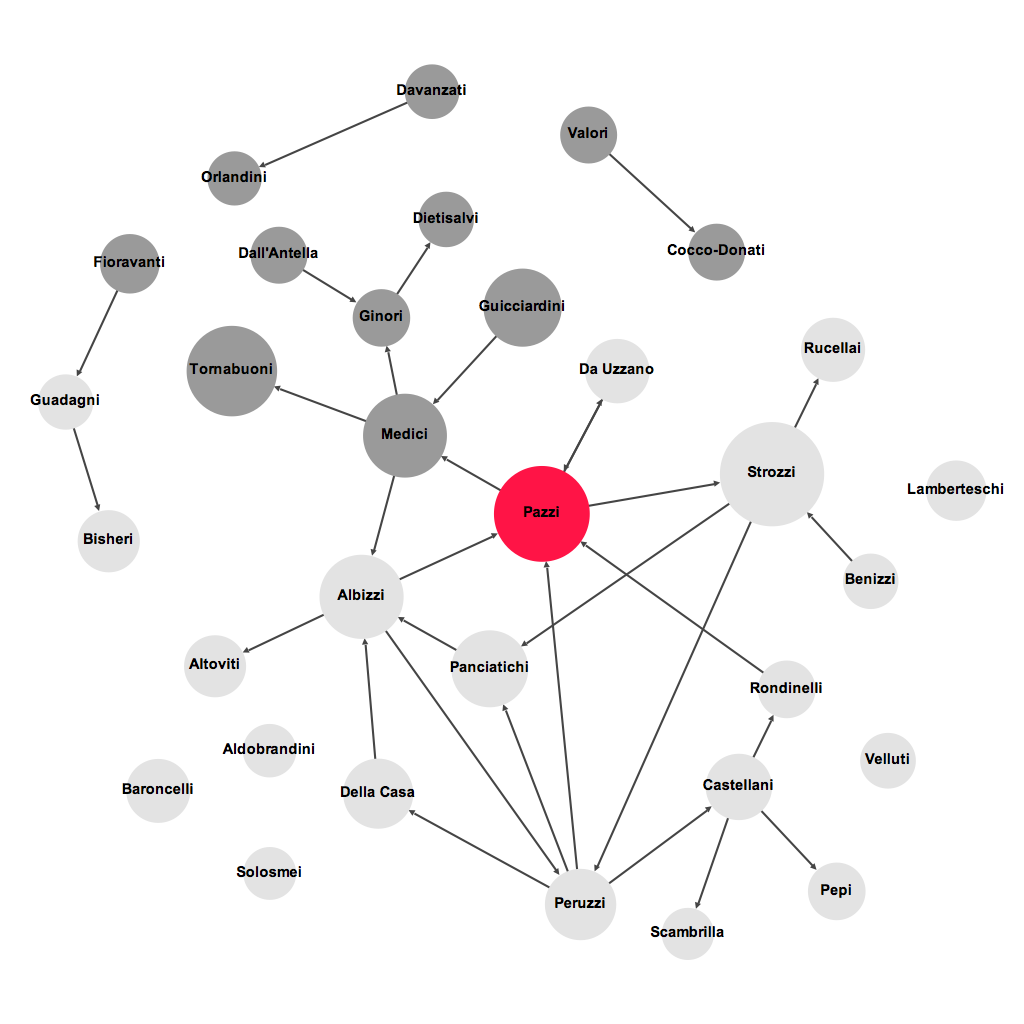
\includegraphics[scale=0.37]{imgs/Florentine-marr.png}
\caption{Directed network of Florentine marriages (c. 1434)}
\label{Fig:FlorentineFamilies}
\end{figure}

It has been shown in contemporary studies of the marriage network that the Medici family have the highest degree, closeness, and betweenness centralities. However, \citet{Roover1963}, \citet{Padgett1994} and \citet{Goldthwaite2009} explain that their importance and power in the marriage network especially is derived from their ability to access diverse sources of information between separate factions of the Florentine elite and subsequently broker relationships between families of separate factions. As such, the Medici family filter information by allowing or not allowing pieces of information to spread to other factions; thus largely monopolising informational spread. Powerful brokerage opportunities, which the Medici took advantage of, emerged due to the inherent ``network disjunctures within the elite'' \citep[p.~1259]{Padgett1993}. In particular, \citet{Padgett1993} show that Cosimo de'Medici was able to gain access to, and control, the flow of diverse information between opposing political factions and also between families in the same faction. Thus, a middleman position allowed the Medici family to attain power within Florentine society; especially, the Medici's ability to act as broker between a large number of families crossing opposing political factions.

Unlike more recent renditions of the Florentine marriage network where the marriage network is depicted as a reduced undirected graph---but keeping in line with the format initially provided by \citet[p.~1276--1277]{Padgett1993}---we represent this network as a directed graph. In doing so we draw an arc from family $i$ to family $j$ to represent a female from family $i$ married into family $j$. The resulting marriage network can be seen in Figure~\ref{Fig:FlorentineFamilies}\footnote{The data was initially gathered by \citet{Kent1978} and a blockmodel network was constructed and used in \citet{Padgett1993} and \citet{Padgett1994}. The network provided in Figure~\ref{Fig:FlorentineFamilies} is derived from these studies. Both provide an extremely rich analysis of the elite in Florence at this time.}. The intuition for this representation is that families were strategically married in order to build trust, inherit wealth, property, and business, as well as influence the political and economic decisions of other families. Information will have flowed through these relationships and these marriage will have often supported economic relationships in the form of trade, employment and loan provision. Moreover, unlike more recent assessments of the Florentine marriage network we include families as groups; thus all nodes represent a group of families under the same name. The groups of families are coloured depending on the factions that the families were affiliated: dark grey nodes are families affiliated with the Medician faction; light grey nodes are families affiliated with the opposing Oligarch faction; and the only family with clear split loyalties (which became increasingly oligarchical over time) is the Pazzi family coloured in red. Finally the size of the node corresponds to the relative cumulative gross wealth of the family in the group: a node of a relatively large size is considered to have a relatively large gross wealth. For reference, the node of the smallest size is the Scambrilla family.

Data was gathered regarding the cumulative gross wealth of groups of all families. This data can be derived from the census and property survey of Florentine dominions in the province of Tuscany, 1427--1480. The data has also been posted online as the \emph{Online Catasto of 1427} and can be found in Appendix B of \citet{Padgett1993}. The Medici family, despite their political and cultural prominence, are only considered as the fifth wealthiest elite family in Florence during this time. The Medici are not even the wealthiest family in their own faction; they are second to the Tornabuoni family. This information expresses two features: first, this was not the zenith period of the Medici; and second, it can be argued that it was specifically the Medici's superior position in the marriage network as opposed to just their economic presence that allowed them to gain command in Florence during this time. Elaborating on the first point we note that although the Medici had established a considerable banking dynasty by 1427 it was still under the command of Giovanni di'Bicci de'Medici. We know from  It wasn't until the reign of Cosimo di'Giovanni de'Medici in 1929 that the House of Medici rose to phenomenal economic and political prominence. The argument made by the second point provides the basis for our discussion regarding the structure of the network and the centrality of families with respect to the strategic marriages.

\subsubsection{Network structure}

There are 11 families in the Medician faction and 21 families in the oligarchic faction. The marriage network contains 9 weakly connected components and 23 strongly connected components. The giant weakly connected component contains 62.5\% of all elite families in the analysis. The network diameter is 6 with an average path length of 2.881 and the directed network density is 0.031. The average degree is 0.969, and the distribution is similar to that of a power law. The maximal $k$-core is 4 and contains the Pazzi, Peruzzi, Strozzi, and Albizzi families: these families form a \emph{rich club}. The network thickness index is 0.

A non-technical analysis of the network produced in Figure~\ref{Fig:FlorentineFamilies} highlights a clear distinction between the connectivity of the two main factions. If we were to include the Pazzi as a member of the Oligarch faction then only $\frac{3}{31}$ of the marriages formed were marriages between families of different factions. It is also clear that the families of the Pazzi, Albizz and Madici are clear gate-keepers to information flows between the factions within the main component. However, the Medici is the only family that acts as a (strong) middleman between both factions; the removal of the Medici leads to the partitioning of the factions in the main component.

The structure of the Medician faction takes the form of a rooted tree---a hierarchical construct---where the Medici family exist at the root. Such a structure provides a better basis for top-down organisation and the distribution of command throughout the elite families. This structure contrasts with the Oligarchic faction where individual agents are more densely connected and thus more structurally equivalent. It was explained that the Oligarchic faction suffered from ill-defined leadership and inter-faction power struggles. This more decentralised structure is certainly reflected in the marriage network. Specifically, \citet{Padgett1993} and \citet{PadgettMcLean2006} noted that the Oligarchic faction was less cohesive and more disorganised than the Medician faction. From our analysis it is seen that there are more brokerage opportunities in the Oligarchic faction highlighting that they were more disjunctured. We see that $\tfrac{7}{16}$ of the connected Oligarchs are middlemen against $\tfrac{2}{11}$ of the families in the Medician faction. Thus, the presence of more middleman positions within the Oligarchs decentralised structure allows for more brokering of information flows and, as such, a greater ability to manipulate information flows between members of the faction. This potential for the manipulation of information derived from the positional attributes of a family was not as prominent a feature within the Medician faction.

Further, we note that when running Newman's Q-measure of network modularity \citep{Newman2004detecting, Newman2006}---which gives the value of 0.521---the different factions can be easily partitioned. More specifically, Oligarchic faction is deconstructed into three distinct communities whereas the Medician faction remains as one district community. Moreover, the partitioning of the communities are determined by the middlemen within the faction. This measure of modularity reinforces the disjunctured nature of the Oligarchic faction. The community structure of the giant weakly connected component can be seen in Figure~\ref{Fig:Florentinemodu} in the appendices of this chapter.

\subsubsection{Centrality and power}

We analyse the resulting directed network in Figure~\ref{Fig:FlorentineFamilies} in a more technical way using in-degree $\left(d^-\right)$, out-degree $\left(d^+\right)$, \citet{Bonacich1987} eigenvector centrality ($E$), betweenness centrality ($BC$), and the normalised middleman power ($\nu$) of each family. The results of the analysis on middlemen is presented in Table~\ref{tabFlorence}. A full table of centrality analysis can be found in Table~\ref{tabFlorenceA} in the appendices of this chapter. In both tables the (*) and (**) after the family's name denotes a weak middleman and strong middleman. Throughout the analysis below we discuss the centrality and power of a family in both the directed and undirected network.

\begin{table}
\begin{center}
\begin{tabu} to \textwidth {X[l]  X[c]  X[c]  X[c]  X[c]  X[c]}
\\[-1.8ex]\hline
\hline \\[-1.8ex]
	            & Gross   &								 &			 &		   &		  \\
Name 		    & wealth  & $d^+_i$ $\left(d^-_i\right)$ & $BC_i$    & $E_i$   & $\nu_i$  \\ \hline
Albizzi(**)     & 249,940 & 3(3) 						 & 0.066 	 & 0.701   & 0.357 	  \\
Castellani(**)  & 111,355 & 3(1) 						 & 0.034 	 & 0.310   & 0.187 	  \\
Ginori(**)      & 42,333  & 1(2) 						 & 0.014 	 & 0.257   & 0.076    \\
Guadagni(**)    & 25,179  & 1(1) 						 & 0.001 	 & 0.001   & 0.006 	  \\
Medici(**)      & 248,105 & 3(2) 						 & 0.058 	 & 0.506   & 0.269 	  \\
Pazzi(**)       & 341,198 & 3(4) 						 & 0.093 	 & 1.000   & 0.503    \\
Peruzzi(*)      & 150,375 & 4(2) 						 & 0.070 	 & 0.612   & 0.287    \\
Rondinelli(*)   & 43,588  & 1(1) 						 & 0.014 	 & 0.157   & 0.076    \\
Strozzi(**)     & 407,296 & 3(2) 						 & 0.053 	 & 0.506   & 0.152    \\ \hline
\end{tabu}%\par
\caption{Analysis of middlemen in the elite marriage network of Renaissance Florence}
\label{tabFlorence}
\end{center}
\end{table}

The simplest measurement of the centrality and power of a node is the number of links it has in a network. In a directed network the connections that a node has can be partitioned into the number of direct successors (node out-degree) and the number of direct predecessors (node in-degree). The Peruzzi family has the greatest number of direct successors (4) and the Pazzi have the greatest number of direct predecessors (4); the Pazzi family also have the greatest sum of direct successors and direct predecessors (7). In an undirected network the connections that a node has is simply the total number of links that a node has; this is not necessarily the same as the sum of direct predecessors and direct successors as some node may be both a direct predecessor and direct successor. If the network were transformed to its undirected form then the Pazzi, the Albizzi, and Peruzzi families are connected to 6 families each. The Medici and Strozzi families are connected to 5 families each. 

There are two aspects to note from the assessment of node degree. First we note that, in general, families with a relatively higher degree are more prone to be middlemen in the network. This is true for most families apart from the Guadagni who are conveniently positioned such that their single in-degree and single out-degree forms a middleman position. Second, we note that the Medici faction does not have the highest degree centrality relative to other families in the Oligrahic faction.

Assessing the marriage network with the middleman power index highlights the Medici family as a strong middleman, along with the prominent Albizzi, Castellani, Ginori, Pazzi, and Strozzi families. It is, however, the Pazzi and Albizzi families that have a greater middleman power (0.503 and 0.357, respectively) than the Medici (0.269). The diversity of the Medici's brokered relationships extend further than those of the Albizzi and Pazzi families as the Medici brokers between factions. If, however, the direct marriage network is transformed into an undirected network such that information can flow in both directions then the Medici becomes the most powerful middleman with a normalised middleman power of 0.470; they are followed by the Ginori, Castellani and Strozzi families who have a normalised middleman power of 0.213. if the marriage network were converted into its undirected form, the Medici retains its strong middleman position maintaining the highest middleman power in the marriage network, and therefore control the flow of information and influence between more families.

The betweenness centrality measure ranks the Pazzi family as the most central in the directed marriage network. The measure favours middlemen thus typically ranking them higher; eight out of the top ten families in terms of their betweenness score are either weak or strong middlemen. In the undirected representation of the network the Medici have the highest betweenness centrality (0.166) followed by the Pazzi (0.142).

Unsurprisingly, the Bonacich centrality measure also ranks the Pazzi family highly, but also ranks many non-middlemen highly; specifically the Panciatichi family. From the network topology alone there is no indication to suggest that the Panciatichi family should have had a prominent role in the Florentine elite. Although the Medici rank highly with this measure, the relevance of an eigenvector centrality measure is questionable: there is no real reason to believe why the importance of a family would come from its degree and the degree of its neighbours alone. However, despite that the eigenvector centrality correlates highly with the gross wealth of the 

\subsubsection{Threshold sets, thickness and middleman robustness}

Due to the low density of the directed marriage network only one elite family---the Panciatichi family---is a non-middleman that can potentially become a middleman from the removal of other families in the network. Specifically, given the removal of the Peruzzi family the Panciatichi family becomes a middleman in the directed network. The Panciatichi family therefore has a thickness of 1. All other nodes either have a thickness of 0, since they can never be a middleman, or a thickness of $\infty$, since they already are middlemen.

We finally discuss the robustness of each middleman position in terms of the $\alpha$-robustness, $\beta$-robustness, and $\gamma$-robustness measures that were developed in this chapter. We provide information on the robustness of middlemen in both the directed and undirected marriage networks and the results can be seen in Table~\ref{FlorenceRobust}. In general we find that the $\beta$- and $\gamma$-robustness measures provide extremely similar results. The directed network highlights the Albizzi and Pazzi families as being robust; especially in terms of the $\beta$-robustness and $\gamma$-robustness measures. Both families are followed by the Medici, who are substantially robust across all measures. The results of the robustness measures suggests that there is a clear distinction between the consistency of some middlemen over others. All robustness measurements provide the same result with respect the the undirected form of the marriage network. The Medici is highlighted as being the most robust strong middleman in the undirected network. Notably, even though the Pazzi and Albizzi were robust in the directed network they both perform poorly in terms of the undirected representation of the marriage network.

\begin{table}[]
\centering
\caption{Robustness analysis of middlemen in Renaissance Florence}
\begin{tabu} to \textwidth {X[l]  X[c]  X[c]  X[c] || X[c]  X[c]  X[c]  X[c]} 
\hline \hline
               &              & Directed    &              &              & Undirected  &              \\
Name           & $\alpha_{i}$ & $\beta_{i}$ & $\gamma_{i}$ & $\alpha_{i}$ & $\beta_{i}$ & $\gamma_{i}$ \\ \hline
Albizzi(**)    & 6            & 3           & 3            & 1            & 1           & 1            \\
Castellani(**) & 3            & 1           & 1            & 2            & 2           & 2            \\
Ginori(**)     & 2            & 1           & 1            & 2            & 2           & 2            \\
Guadagni(**)   & 1            & 1           & 1            & 1            & 1           & 1            \\
Medici(**)     & 6            & 2           & 2            & 3            & 3           & 3            \\
Pazzi(**)      & 6            & 3           & 3            & 1            & 1           & 1            \\
Peruzzi(*)     & 2            & 2           & 2            & 0            & 0           & 0            \\
Rondinelli(*)  & 1            & 1           & 1            & 0            & 0           & 0            \\
Strozzi(**)    & 4            & 2           & 2            & 2            & 2           & 2            \\ \hline
\end{tabu}
\label{FlorenceRobust}
\end{table}

The robustness and centrality measures do not highlight the factions that exist within this network, and therefore simply assumes that relationships can be made without social or institutional pressures. As a consequence it could be argued that, regardless of the robustness measures, the Medici has the highest middleman robustness due to the fact that they are middlemen across both factions. Indeed, social and marriage relationships cannot be formed so seamlessly between families of opposing factions, therefore the robustness of the Medici's position is further strengthened due to the institutional pressures of society itself. This is, as previously discussed, a convincing reason for why the Medici's powerful position was stable for such a long time.

\medskip\noindent The Medici attained control in Florence because they not only brokered relationships between elite families in the network, but because they brokered relationships between two opposing factions. Therefore, they were not only able to gather and intercept information between the factions but also use it to their advantage. This is the prerogative of middlemen in social networks; to not only intercept and facilitate information between agents, but to manipulate and exploit it.

\begin{figure}[t]
\centering
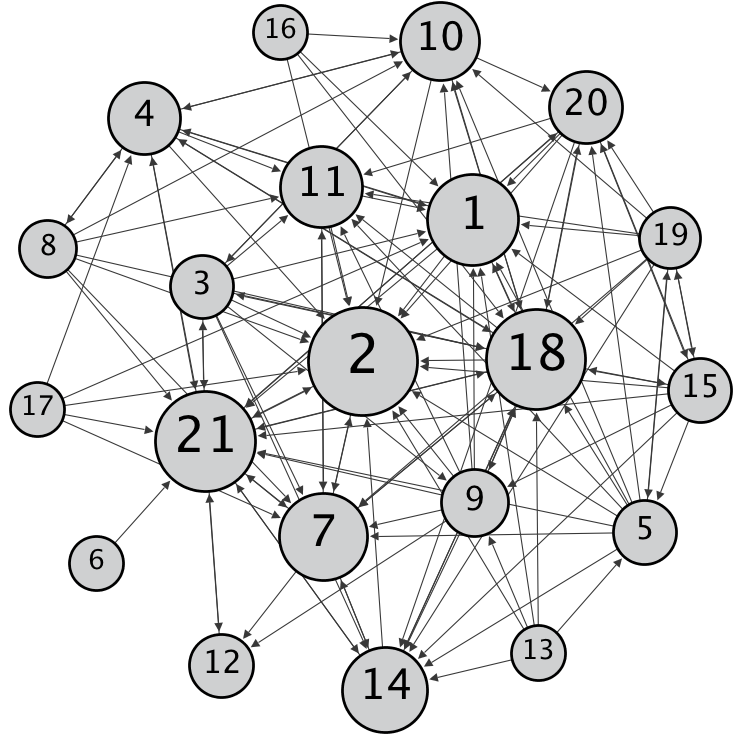
\includegraphics[scale=0.45]{imgs/krack.png}
\caption{Krackhardt's network of advice among managers}
\label{krackhardtnetwork}
\end{figure}

\subsection{Middlemen in Krackhardt's advice network}

Next we consider an example of a well-known organisational advice network in which \citet{Krackhardt1987} investigated the relationships between managers in a given firm\footnote{We use data in the ``LAS'' matrix from p.~129 in the Krackhardt article as it seems to be the most objective measure.}. He considered an organisation of about 100 employees and 21 managers. Krackhardt collected information from the managers about who sought advice from whom, depicted in Figure~\ref{krackhardtnetwork} on page \pageref{krackhardtnetwork}. An arc from $i$ to $j$ denotes that manager $i$ has sought advice from manager $j$; therefore, an arc from $j$ to $i$ denotes that manager $j$ has provided advice to manager $i$. In this depiction the size of the node reflects its in-degree.

\begin{table}[h]
\begin{center}
\label{tabkrackhardt}
\begin{tabu} to \textwidth {X[l]  X[c]  X[c]  X[c]  X[c]  X[c]}

\\[-1.8ex]\hline
\hline \\[-1.8ex]
Manager       & $d^-_i$ $\left(d^+_i\right)$& $E_i$    & $BC_i$   & $\nu_i$  & $\nu_{i}^{*}$\\ \hline
1             & 12 (4)           & 0.068    & 0.035    & 0.000    & 0.000		 \\
2             & 18 (2)           & 0.306    & 0.011    & 0.000    & 0.000		 \\
3             & 3 (9)            & 1.271    & 0.018    & 0.000    & 0.000		 \\
4(*)          & 6 (7)            & 1.001    & 0.071    & 0.090    & 0.034		 \\
5             & 3 (10)           & 1.463    & 0.009    & 0.000    & 0.000		 \\
6             & 0 (1)            & 0.172    & 0.000    & 0.000    & 0.000		 \\
7             & 11 (6)           & 0.776    & 0.048    & 0.000    & 0.000		 \\
8             & 1 (7)            & 1.013    & 0.001    & 0.000    & 0.000		 \\
9             & 4 (9)            & 1.171    & 0.011    & 0.000    & 0.000		 \\
10            & 8 (5)            & 0.820    & 0.018    & 0.000    & 0.000		 \\
11            & 9 (3)            & 0.344    & 0.004    & 0.000    & 0.000		 \\
12            & 3 (1)            & 0.172    & 0.000    & 0.000    & 0.000		 \\
13            & 0 (6)            & 0.938    & 0.000    & 0.000    & 0.000		 \\
14            & 10 (4)           & 0.625    & 0.002    & 0.000    & 0.000		 \\
15(*)         & 3 (9)            & 1.265    & 0.092    & 0.161    & 0.064		 \\
16            & 0 (4)            & 0.580    & 0.000    & 0.000    & 0.000		 \\
17            & 0 (5)            & 0.673    & 0.000    & 0.000    & 0.000		 \\
18            & 15 (12)          & 1.745    & 0.231    & 0.000    & 0.000		 \\
19            & 2 (10)           & 1.493    & 0.002    & 0.000    & 0.000		 \\
20            & 6 (7)            & 1.028    & 0.028    & 0.000    & 0.000		 \\
21(**)        & 15 (8)           & 1.348    & 0.176    & 0.147    & 0.051		 \\ \hline
\end{tabu}
\caption{Influence, centrality, and middlemen in Krackhardt's advice network}
\end{center}
\end{table}

In Table 4, using the same centrality measures as before, we identify two weak middlemen, managers 4 and 15, and one strong middleman, manager 21\footnote{As before, (*) indicates a weak middleman and (**) indicates a strong middleman.}. Middlemen are important for this network for a number of intuitive reasons: First, a middleman can block ideas, advice, and information from being transmitted from one group of managers to another. Second, a middleman can manipulate the information transferred from one group of managers to another.

The weak middleman, Node 15, has the highest brokerage in the organisation controlling a total of 34 relationships. This is also reflected in that \citet{Krackhardt1987} highlighted manager 15 as an important agent in the organisational advice network. However, Node 15 does not have the highest betweenness or Bonacich centralities. Instead, Node 18 is the most prominent in terms of Bonacich and betweenness scores but is not a middleman in the network; instead this may be a function of the in- and out-degree of node 18.

Both Bonacich and betweenness centralities are also seen to be poor indicators for ranking middlemen: Node 15 is the most powerful middleman in the network, but has a Bonacich and betweenness centrality lower than Node 21. The Bonacich influence model does not consider the fact that middlemen are potentially able to exploit their position by using information from others and blocking the transmission of certain information and ideas.

\subsubsection{Concluding comments}

Due to the formation of new socio-economic roles entrepreneurial agents can assume unique positions in a network. These unique positions can intuitively be seen with respect to their connectivity in the socio-economic space and can be defined accurately as middleman positions. Positioning oneself in a unique way in the socio-economic space is the essence of a network entrepreneur as discussed in chapter~\ref{ch:entrepreneurship}. Middlemen possess an ability to connect pairs of agents who would otherwise be disconnected from each other; these can have liberating externalities for those directly or indirectly connected to middlemen in the form of opening new exchange routes and channels of information, but middlemen can exploit their position and as such act in a highly extractive way to their neighbourhood. Whether a middleman behaves in an exploitive or facilitating manner is ambiguous and not covered here, however the middleman power measure provides a mechanism in which to measure the positional power of the middleman and therefore provides a quantitative value to the potentially extractive nature of the agent.

The assessment of middlemen is purely individualised. We can extend the assessment to collective economic interaction and thus cooperative economic activities to include coalitions of economic agents who as a whole form a middleman position in a network.


\begin{subappendices}

\section{Power and centrality tables for Renaissance Florence networks} \label{A}

\begin{table}
\begin{center}
\begin{tabu} to \textwidth {X[l]  X[r]  X[c]  X[c]  X[c]	X[c]  X[c]}
\\[-1.8ex]\hline
\hline \\[-1.8ex]
          & Gross  &  &  &  & \\
Family 			    & wealth & $d^+_i$ $\left(d^-_i\right)$   	&  $BC_i$		&  $E_i$		&  $\nu_i$        \\ \hline
Albizzi(**)     & 249,940 & 3(3) & 0.066 & 0.701 & 0.357      \\
Aldobrandini    & 10,805  & 0(0) & 0.000 & 0.000 & 0.000      \\
Altoviti        & 77,621  & 0(1) & 0.000 & 0.355 & 0.000      \\
Baroncelli      & 92,615  & 0(0) & 0.000 & 0.000 & 0.000      \\
Benizzi         & 26,093  & 1(0) & 0.000 & 0.000 & 0.000      \\
Bisheri         & 78,729  & 0(1) & 0.000 & 0.002 & 0.000      \\
Castellani(**)  & 111,355 & 3(1) & 0.034 & 0.310 & 0.187      \\
C-Donati        & 37,260  & 0(1) & 0.000 & 0.001 & 0.000      \\
Da Uzzano       & 96,131  & 1(1) & 0.000 & 0.506 & 0.000      \\
Dall'Antella    & 37,914  & 1(0) & 0.000 & 0.000 & 0.000      \\
Davanzati       & 19,887  & 1(0) & 0.000 & 0.000 & 0.000      \\
Della Casa      & 140,624 & 1(1) & 0.001 & 0.309 & 0.000      \\
Dietisalvi      & 26,274  & 0(1) & 0.000 & 0.132 & 0.000      \\
Fioravanti      & 57,674  & 1(0) & 0.000 & 0.000 & 0.000      \\
Ginori(**)      & 42,333  & 1(2) & 0.014 & 0.257 & 0.076      \\
Guadagni(**)    & 25,179  & 1(1) & 0.001 & 0.001 & 0.006      \\
Guicciardini    & 203,087 & 1(0) & 0.000 & 0.000 & 0.000      \\
Lamberteschi    & 64,775  & 0(0) & 0.000 & 0.000 & 0.000      \\
Medici(**)      & 248,105 & 3(2) & 0.058 & 0.506 & 0.269      \\
Orlandini       & 16,315  & 0(1) & 0.000 & 0.001 & 0.000      \\
Panciatichi     & 193,878 & 1(2) & 0.005 & 0.566 & 0.000      \\
Pazzi(**)       & 341,198 & 3(4) & 0.093 & 1.000 & 0.503      \\
Pepi            & 43,100  & 0(1) & 0.000 & 0.157 & 0.000      \\
Peruzzi(*)      & 150,375 & 4(2) & 0.070 & 0.612 & 0.287      \\
Rondinelli(*)   & 43,588  & 1(1) & 0.014 & 0.157 & 0.076      \\
Rucellai        & 93,891  & 0(1) & 0.000 & 0.256 & 0.000      \\
Scambrilla      & 148     & 0(1) & 0.000 & 0.157 & 0.000      \\
Solosmei        & 5,757   & 0(0) & 0.000 & 0.000 & 0.000      \\
Strozzi(**)     & 407,296 & 3(2) & 0.053 & 0.506 & 0.152      \\
Tornabuoni      & 299,878 & 0(1) & 0.000 & 0.257 & 0.000      \\
Valori          & 37,842  & 1(0) & 0.000 & 0.000 & 0.000      \\
Velluti         & 28,108  & 0(0) & 0.000 & 0.000 & 0.000      \\ \hline
\end{tabu}%\par
\caption{Measuring the importance of Florentine families (c. 1434)}
\label{tabFlorenceA}
\end{center}
\end{table}



\begin{figure}[t]
\centering
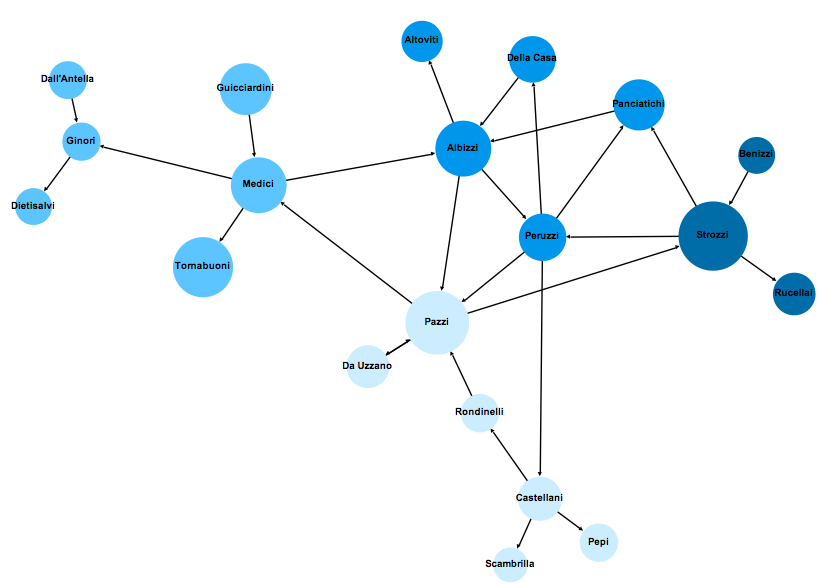
\includegraphics[scale=0.4]{imgs/Florentine-modu.png}
\caption{Community structure detection on elite Florentine marriages}
\label{Fig:Florentinemodu}
\end{figure}

\end{subappendices}
\chapter{The formation of extractive structures in networks}
\label{ch:blocks}

In extending the notions discussed in Chapter~\ref{ch:criticalnodes} we investigate how sets of economic agents in certain network positions can manipulate flows of information and traded goods in the network and extract rents from their position. The resulting extractive structures affect many processes in our globalised economy, such as investment and loan provision \citep{Gai2010, ElliotGolubJackson2014}, shareholdings and corporate ownership \citep{Vitali2011}, learning and information dissemination \citep{GolubJackson2010}, advice and influence \citep{Krackhardt1987}, as well as favour exchange \citep{Jackson2012}.

\subsection{A motivating example: The Florentine elite in the 15th Century}

To motivate our discussion we return to the well-known network of elite marriages in Florence, Italy circa 1435 \citep{Kent1978,Padgett1993}. Such marriages were the main political instrument to exert control and build trust among the major houses that make up the Florentine elite. It is clear that even though these Florentine houses had other social relations, a marriage indicated a high degree of trust and transparency between the two houses that were party to it.

As above, the collection of marriage relationships between the various medieval Florentine houses as a directed network rather than an undirected network. In the network depicted in Figure~\ref{Flocrit} an arc $ij$---represented by an arrow from node $i$ to node $j$---describes that a male in house $i$ marries a female in house $j$. Such an arrow represents the likely flow of information between the two houses: A female gathered information regarding the house $i$ into which she married and pass it back to the house $j$ from which she originated.

From the directed network representation of these marriage relationships, we can glean the power and control exerted by the various houses in medieval Florence. The resulting network analysis should corroborate the historical evidence of power brokerage in medieval Florence. In particular, there were two opposing factions in the Florentine society in the 15th Century: The \emph{Medician} and the \emph{Oligarchic} factions. There was a long-standing power struggle between both factions, but also \emph{within} both factions houses were striving for control. The opposing factions are highlighted in Figure~\ref{Flocrit}: The Medician faction consists of the dark grey nodes and the Oligarchic faction are represented as the light gray nodes in Figure~\ref{Flocrit}.
\begin{figure}[h] \label{Flocrit}
\begin{center}
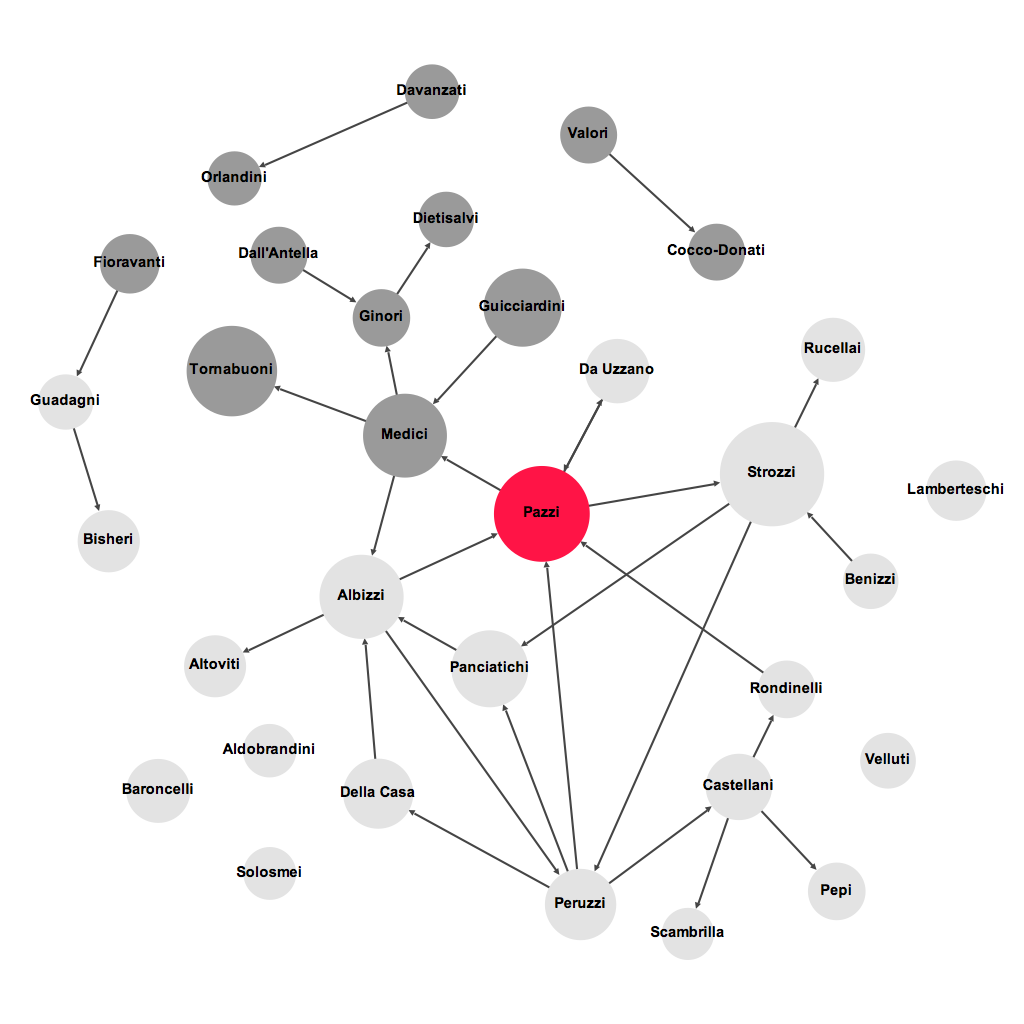
\includegraphics[width=0.9\textwidth]{imgs/Florentine-marr.png}
\end{center}
\caption{The Florentine marriage network}
\end{figure}
Historical analysis by \citet{Roover1946, Roover1963}, \citet{Padgett1993}, and \citet{Goldthwaite2009} attribute the success of the Medician faction during this time to how well organised the Medician faction was relative to the Oligarchic faction. \citet{Padgett1993} suggest that it was common for a member of the oligarchic faction to attempt to overthrow the leadership of its faction and filter information shared with other members. These are indications that there existed a power struggle within the Oligarchic faction. It may be reasonable to assume that more middlemen exist in the Oligarchic faction than the Medician faction. Indeed, when considering the directed network we identify that more middlemen exist in the oligarchic faction where power is more distributed. Conversely, in the Medician faction, power is more centralised in the House of Medici itself. Below we look at each faction individually and analyse middleman power in each reduced network.

It is well accepted that much power was held by the House of Medici, during much of the 15th Century until the Medicis were banished from Florence due to inappropriate lending, leading to war. There are many reasons for the Medici reign, one of which was that the Medician faction was well organised. There existed a hierarchical organisation that centred around the House of Medici with little power attributable to other member houses of the Medician faction.

This is confirmed in the depicted network: The Medici were positioned at the centre of a star. Although the House of Salviati also has a middleman position, it is clear that the Medici control the Salviati; indeed, the Medici had the ability of separating the Salviati from the rest of the faction.

The Oligarchic faction were less well-organised. The faction acted more disruptively as power was more distributed throughout the network; this is illustrated by the widespread presence of middlemen in this network. Consequently, it was less centralised with multiple competing houses at various local power centres. In particular, the Houses of Guadagni, Bischeri, Peruzzi, and Castellan all occupy critical nodes in Figure~\ref{Flocrit}. Therefore, up to half of the faction have the potential to control certain channels of communication. Furthermore, the houses of Peruzzi and Strozzi have an incentive to form a coalition to control information flows in the Oligarchic subnetwork.

Therefore, there exists more opportunities for power struggles in the oligarchic faction than the Medician faction. This is representative of the time. It is worth noting that a power struggle occurred within the Medician faction later with respect to the \textit{Pazzi Conspiracy}. And this is conducted through the intervention of the Salviati house, which intermediates the Pazzi and Medici houses in the network.

\paragraph{Chapter outline.}

In this chapter we introduce analytical concepts that try to measure these features in any arbitrary directed network. These concepts are supported by two analytical methods, one based on identifying contestation of critical node sets and the other founded in a non-cooperative game theoretic analysis that identifies the stable critical structures that emerge in a network. We report that the resulting measures corroborate the historical analysis of the medieval Florentine marriage network presented above.

\subsection{Relationship to the literature}

The work here broadly applies the notions of critical nodes and node cut sets, originally developed in graph theory, to situations in economics and sociology. In social and economic terms, the graph theoretic notion of a critical node is analogous to that of a \emph{middleman}. There exists much work assessing the importance of critical nodes in economics. We specifically note seminal work developed by \citet{KalaiMiddlemen1978} which was extended by \citet{JacksonWolinsky1996} and further elaborated upon by \citet{GillesChakrabarti2006} with respect to undirected networks. This literature showed that middleman positions are important in networked intermediation and that such critical nodes can extract significant gains from their positions within a cooperative game theoretic framework. Indeed, the insights were analogous to those found by \citet{RubinsteinWolinsky1987}. There also exists much work in sociology regarding critical nodes and power. \citet{Emerson1962} illustrates a theory of power relations by assessing the dependence of each player on the other, and thus the number of alternatives that each player has at their disposal for the achievement of a given task. The notions of power--dependence relations were extended to analyse the power of agents in exchange networks by \citet{CookEmersonGillmoreYamagishi1983}. \citet{GouldFernandez1989} note that there can exist multiple types of broker, which acts as a critical node, and provide quantitative measurements for these nodes primarily based on the notion of betweenness centrality. \citet{Gould1989} builds on these early insights, developing a measure for an agents inter--clique brokerage. More recent research has investigated more dynamics of brokerage \citep{Spiro2013}. Despite the vigorous research from both fields into the interlinked notions of middlemen, brokerage, and critical nodes, he notion of node cut sets still require intuitive application to scenarios in both sociology and economics. This article provides one application of cut sets in the form of block formation.

Exploitation and power is closely related to the notion of \emph{competition} in economic systems. Competition has been at the heart of market theory and traditional economics since the formal introduction of Bertrand competition, which claims that if there exists two or more producers for some homogeneous product in a given market then the producers will continually reduce their price levels so that all producers are selling their outputs at the marginal cost of production. The assumption of competitive systems is at the heart of both micro and macroeconomic modelling, however there does not yet exist a broad range of literature regarding competition in networked markets.

\citet{EasleyKleinberg2010} provide a baseline model regarding three classes of players exchanging with each other in a tripartite network subsequently highlighting potential notions of perfect competition and monopolisation. These competitive notions are built from a combination of Bertrand competition and more implicitly from insights of power introduced by \citet{Emerson1962}. \citet{GillesDiamantaris2013} note the importance of middlemen, or \emph{platforms}, regarding their ability to extract rents from its users that use the platform to interact. The previous chapter provided a formal definition of both strong and weak middlemen in directed networks and in doing so turn applying this to a network--centric notion of competition which is effectively a generalisation of Easley and Kleinberg's notion of competition.

\citet{GoyalVega-holes} provides an elaborate example of network formation with surplus--generating economic exchange. The surplus from exchange is split evenly between players that are directly connected and any indirect exchange is split with the set of intermediaries. Players that span structural holes, \'{a} la \citet{Burt1992}, can therefore be highly extractive depending on the players whose exchange they intermediate.

To this point there is a serious deficiency regarding groups of agents collectively attaining extractive positions in networks, comparable to the notion of a \emph{cartel} in economic theory. A procedure proposed by \citet{Aspremont1983} studies the formation of a cartel whereby players announce their willingness to participate in the cartel. A cartel is formed by all players that have announced their willingness to do so. The equilibria of the cartel formation game is characterised by internal and external stability. A cartel is internally stable if no members of the cartel wish to leave, and a cartel is externally stable if no outsider wishes to join the cartel. Drawbacks of the study include that the formation of only a single cartel is considered, and there exists no insights from networks. The integration of a network provides an insightful take on the incentives of cartel formation. Furthermore, we extend the concept to include transfers between players.

We note that the formation of blocks in networks is analogous to the formation of cartels in market economies. However, when applied to networks we find that there can emerge situations where monopolists have an incentive to form a block with other monopolists as well as other powerless players.

\section{Extractive structures in networks}

We introduce the concepts that describe extractive structures in a directed network.

\subsection{Social networks: Basic concepts}

We set out some basic definitions from network theory. The concepts and notation are mainly taken from \citet{Jackson2008}. Other standard sources on network theory are \citet{Newman2006book}, \citet{Goyal2007}, \citet{Newman2010} and \citet{Gilles2010}.

We consider a \emph{directed network} as a pair $(N,D)$ where $N=\{1 , 2 , \ldots , n\}$ is a finite set of \emph{nodes}, embodying self-motivated decision-makers, and $D \subset \{(i,j) \mid i,j \in N \mbox{ and } i \neq j\}$ is a set of \emph{arcs}, representing directed links from one node to another.\footnote{We use the notational convention that for two sets $S$ and $T$, we denote by $S \subset T$ that $S$ is included as a subset in $T$ or that $S=T$. Strict inclusion is denoted by $S \subsetneq T$.}

An arc from node $i$ to node $j$ is also denoted by $ij = (i,j)$ which is distinct from $ji = (j,i)$. We remark that our analysis can equally be applied to undirected networks in which all arcs are reciprocated such that $ij \in D$ if and only if $ji \in D$ for all $i,j \in N$.

A \textit{walk} from $i$ to $j$ in a directed network $D$---or an $ij$--\textit{walk}---is an ordered set of nodes $W_{ij} = \{ i_{1}, \ldots ,i_{m} \} \subset N$ with $m \geq 2$, $i_1 =i$, $i_m =j$, and $i_{k}i_{k+1} \in D$ for all $k=1, \ldots ,m-1$. An $ij$--walk $W_{ij}$ from node $i$ to node $j$ in network $D$ is a $ij$--\textbf{path} if there is no $ij$--walk $W'_{ij}$ in $D$ such that $W'_{ij} \subsetneq W_{ij}$. Hence, a path from $i$ to $j$ is a walk from $i$ to $j$ without any loops or cycles.\footnote{This implies that the removal of a node from a $ij$--path will break the connection between $i$ and $j$.}

In many cases there exist multiple paths from $i$ to $j$ in a directed network $D$. Therefore, we denote $W_{ij}^{v}$ as the $v^{th}$ distinct path from $i$ to $j$ in $D$. The class $\mathcal{W}_{ij} (D) = \left\{ W_{ij}^{1}, \ldots ,W_{ij}^{V} \right\}$ consists of all distinct paths from $i$ to $j$ in $D$, where $V = \# \mathcal{W}_{ij}(D)$ is the total number of distinct paths.  If there are no paths from $i$ to $j$, i.e., $V=0$, then $\mathcal{W}_{ij}(D)= \varnothing$. An $ij$--path is a \emph{geodesic path} from $i$ to $j$ in $D$ if it is the path in $\mathcal{W}_{ij} (D)$ with the least number of nodes.

The directed network $D$ is (weakly) \emph{connected} if $\mathcal{W}_{ij}(D) \neq \varnothing$ or $\mathcal{W}_{ji}(D) \neq \varnothing$ or both for all nodes $i,j \in N$. The network $D$ is \emph{strongly connected} if $\mathcal{W}_{ij}(D) \neq \varnothing$ as well as $\mathcal{W}_{ji}(D) \neq \varnothing$ for all nodes $i,j \in N$. Clearly, strongly connected networks are always connected and connected undirected networks are necessarily strongly connected.

If $\mathcal{W}_{ij} (D) \neq \varnothing$, then $j$ is denoted as a \textit{successor} of $i$ in $D$ and $i$ is denoted as a \textit{predecessor} of $j$ in $D$. We let $S_{i}(D)= \{j \in N \mid \mathcal{W}_{ij}(D) \neq \varnothing \}$ as $i$'s \textit{successor set}, where $i \notin S_{i}(D)$. Also, we let $\overline{S}_{i}(D) = S_{i}(D) \cup \{i\}$. Finally, we define $s_{i}(D) = \left\{\, j \in N \,\middle|\, (i,j) \in D \,\right\}$ as the set of \textit{direct successors} of $i$ in $D$. Likewise, $P_{i}(D)=\{j \in N \mid \mathcal{W}_{ji}(D) \neq \varnothing \}$ denotes $i$'s \textit{predecessor set}, where $i \notin P_{i}(D)$ and $\overline{P}_{i}(D) = P_{i}(D) \cup \{i\}$. Here, $p_{i}(D)=\{j \in N \mid (j,i) \in D\}$ is the set of \textit{direct predecessors} of $i$ in $D$.

For a connected network $D$, the node set $N$ can be partitioned into three node classes: Sources; Sinks; and Intermediaries. Node $i \in N$ is a \textbf{source} if $S_{i}(D) \neq \varnothing$ and $P_{i}(D) = \varnothing$; node $i \in N$ is a \textbf{sink} if $S_{i}(D) = \varnothing$ and $P_{i}(D) \neq \varnothing$; and node $i \in N$ in an \textbf{intermediary} if $S_{i}(D) \neq \varnothing$ as well as $P_{i}(D) \neq \varnothing$. In particular, the set of intermediaries in $D$ is introduced as
\begin{equation}
M_D = \{ i \in N \mid S_{i}(D) \neq \varnothing \mbox{ as well as } P_{i}(D) \neq \varnothing \}
\end{equation}
Finally, for any subset of nodes $B \subset N$, we let $D-B$ be defined by
\begin{equation}
D - B = D_{N \setminus B} = \left\{ (j,h) \in D \mid j,h \in N \setminus B \right\} .
\end{equation}
Therefore, $D - B$ is the \emph{restricted} network that results from removing the node set $B$ and all arcs to and from the nodes in $B$.

\subsection{Critical nodes and sets}

Power in social and economic networks tends to rest on individual nodes and sets of nodes that have an ability to broker relationships and control the flows that occur between nodes in a directed network. These nodes and node sets are known as ``critical''.
\begin{definition} \label{Block}
Let $D$ be a directed network on node set $N$ and let $i,j,h \in N$ be distinct nodes.
\begin{abet}

\item A subset of nodes $B \subset N$ is an $ij$--\textbf{critical set} in $D$ if $B \subset \cup \mathcal{W}_{ij}(D) \setminus \{i,j\}$ and $B \cap W_{ij} \neq \varnothing$ for every $ij$--path $W_{ij} \in \mathcal{W}_{ij}(D)$.

\item Node $h$ is an $ij$--\textbf{critical node} in $D$ if the singleton set $\{ h \}$ is a $ij$--critical set in $D$.

\item The collection of critical sets in the network $D$ is given as
\begin{equation}
\mathcal{B}(D) = \left\{ B \subset M_D \mid B \subset N \mbox{ is an $ij$--critical set for some } i,j \in N \, \right\} .
\end{equation}
Also, the set of critical nodes in the network $D$ is defined by
\begin{equation}
\mathcal{M}(D) = \left\{ h \in M_D \mid h \mbox{ is an $ij$--critical node for some } i,j \in N \, \right\} .
\end{equation}

\end{abet}
\end{definition}
An $ij$--critical node set consists of $ij$--intermediaries that control all flows, communication or intermediation between nodes $i$ and $j$ in network $D$. This implies that these nodes can exercise some form of control in the interaction between the nodes $i$ and $j$.

A critical node is a singleton critical set for some pair of nodes. This implies that such a node exercises complete control over all interaction between these two nodes in the network. A critical node is also referred to as a ``middleman'' in the literature.

Definition~\ref{Block} has equal application to undirected as well as directed networks. A critical node set may also contain a middleman or multiple middlemen, but that is not necessary. Also, in an undirected network a critical node set is equivalent to a cut set which removal partitions a network into multiple connected components. In particular, a middleman is a cut node in an undirected network.

\begin{figure}[t]
\begin{center}
\begin{tikzpicture}[scale=0.65]
\draw[thick, ->] (0,2.5) -- (4.4,4.5);
\draw[thick, ->] (0,2.5) -- (4.4,0.4);
\draw[thick, ->] (5,5) -- (9.3,5);
\draw[thick, ->] (5,0) -- (9.3,0);
\draw[thick, ->] (5,5) -- (9.3,0.5);
\draw[thick, ->] (10,5) -- (14.3,2.8);
\draw[thick, ->] (10,0) -- (14.3,2.2);
\draw[thick, ->] (15,2.5) -- (19.3,2.5);

\draw (0,2.5) node[draw,circle,fill=white] {$1$};
\draw (5,5) node[draw,circle,fill=red!40] {$2$};
\draw (5,0) node[draw,circle,fill=white] {$3$};
\draw (10,5) node[draw,circle,fill=white] {$4$};
\draw (10,0) node[draw,circle,fill=red!40] {$5$};
\draw (15,2.5) node[draw,circle,fill=red!40] {$6$};
\draw (20,2.5) node[draw,circle,fill=white] {$7$};

\draw[thick, color=blue!60!black,rounded corners] (9,-1) rectangle (11,6) ;
\draw[color=blue!75!black] (10,2.5) node {$B_2$} ;

\draw[thick, color=blue!60!black,rounded corners] (4,-1) rectangle (6,6) ;
\draw[color=blue!75!black] (5,2.5) node {$B_1$} ;

\end{tikzpicture}
\end{center}
\caption{Illustration of critical sets in a network}
\label{Net1}
\end{figure}

\begin{example} \label{ex:Figure1}
To illustrate the concepts introduced here, consider the directed network depicted in Figure 2 on node set $N = \{ 1,2,3,4,5,6,7 \}$. There are three middlemen---or singleton critical sets---in this network, namely node 2 is a $14$--middleman, node 5 is a $36$--middleman and node 6 is a $i7$--middleman for any $i \in \{ 1,2,3,4,5 \}$. These middlemen are represented as the red-shaded nodes in Figure 2.
\\
We also indicate two other critical sets, both supersets of singleton critical sets. The critical set $B_1 = \{ 2,3 \}$ completely controls all connections from node 1 to all other nodes in this network. Similarly, $B_2 = \{ 4,5 \}$ controls the connections of all nodes in $\{ 1,2,3 \}$ with the nodes 6 and 7.
\\
Finally, we mention that connected nodes can form a critical set. Indeed, $B_3 = \{ 2,5 \}$ controls all interaction between nodes in $\{1,3 \}$ and all nodes in $\{ 4,6,7 \}$ and, therefore, is a critical set.
\end{example}
A number of characteristics can be derived for critical sets in a directed network. We state the next properties without proof.
\begin{property} \label{prop:blocks}
Let $D$ be a network on node set $N$ and let $i,j \in N$ with $i \neq j$.
\begin{itemize}
\item[(i)] A node $h \in N$ is a $ij$--critical node in $D$ if and only if
\[
h \in \left[ \, \cap \mathcal{W}_{ij} (D) \, \right] \setminus \{i,j\} .
\]

\item[(ii)] The critical collection $\mathcal{B} (D)$ on network $D$ has properties similar to a \emph{filter} on the set of intermediaries $M_D \subset N$ in the sense that if $B \subset M_D \setminus \{ i,j \}$ is an $ij$--critical set in $D$, then any $B' \subset N$ with $B \subset B' \subset M_D \setminus \{ i,j \}$ is an $ij$--critical set in $D$.

\item[(iii)] Critical sets can be defined in terms of their connectivity role in the network:
\\
If $B \subset N$ is an $ij$--critical set, then it holds that $\mathcal{W}_{ij}(D) \neq \varnothing$ and $\mathcal{W}_{ij}(D - B) = \varnothing$.

\item[(iv)] Let $h \in N$ be an $ij$--critical node and $B \subset N$ such that $h \in B$. Then, $B$ is an $ij$--critical set if and only if $i,j \notin B$.
\end{itemize}
\end{property}
The following theorem addresses the existence of critical sets in a network.
\begin{theorem} \label{thm:noblock}
Let $D$ be a (weakly) connected directed network on $N$. Then $\mathcal{B} (D) \neq \varnothing $ if and only if there exist $i,j \in N$ with $i \neq j$ with a geodesic distance of at least 3, i.e.,
\begin{equation}
\min \left\{ \left. \# W_{ij} \, \right| \, W_{ij} \in \mathcal{W}_{ij} (D) \right\} \geqslant 3 .
\end{equation}
\end{theorem}
\begin{proof}
Let $B \subset N$ be some arbitrary node set. From its definition we deduce that for $B$ to be a critical set between two nodes $i,j \in N$, $i \neq j$, it must be that for all $i,j \notin B \colon B \cap W_{ij}(D) \neq \varnothing$ for every $W_{ij}(D) \in \mathcal{W}_{ij}(D)$. 
\\[1ex]
\textbf{Only if:} Suppose to the contrary that $\min \left\{ \# W_{ij} \mid W_{ij} \in \mathcal{W}_{ij}(D) \right\} = 2$. This is the case where $j \in S_{i}(D)$ and, thus, $i \in P_{j}(D)$. Let $W^{\min}_{ij} \in \arg\min \left\{ \# W_{ij} \mid W_{ij} \in \mathcal{W}_{ij}(D) \right\}$ be a geodesic path from $i$ to $j$. Clearly, $\# W^{\min}_{ij}(D) = 2$ implies that $W_{ij}^{\min} \setminus \{i,j\} = \varnothing$. Therefore, $\cap \mathcal{W}_{ij} (D) \setminus \{ i,j \} = \varnothing$ meaning that both there are no nodes to form a critical set for $i$ and $j$.
\\[1ex]
\textbf{If:} Suppose that there exists some $i,j \in N$ where $i \neq j$ such that $\min \left\{ \#W \mid W \in \mathcal{W}_{ij}(D) \right\} \geqslant 3$. Then for every $ij$-path $W \in \mathcal{W}_{ij} (D)$ there exists some node $h_W \in N$ such that $h_W \in W \setminus \{i,j\}$. Define
\begin{equation}
B_{ij} = \left\{ h_W \, \left| \, W \in \mathcal{W}_{ij} (D) \, \right. \right\} \subset N \setminus \{ i,j \} .
\end{equation}
We claim that $B_{ij}$ is a $ij$--critical set in $D$. Indeed, note that for any $ij$--path $W \in \mathcal{W}_{ij} (D)$ it holds that $h_W \in B_{ij} \cap W \neq \varnothing$.
\\[1ex]
This concludes the proof of Theorem \ref{thm:noblock}.
\end{proof}

\bigskip\noindent
We note that this insight identifies an extremely weak requirement for the existence of critical sets in a network. The corollary below indicates this and follows from Theorem~\ref{thm:noblock}.
\begin{corollary}
The following properties hold:
\begin{itemize}
\item[(i)] Let $D$ be any incomplete, non-empty network with at least $3$ nodes that are all connected by a path. Then $\mathcal{B} (D) \neq \varnothing$.

\item[(ii)] $\mathcal{B} (D) = \varnothing$ for both the empty and complete networks.
\end{itemize}
\end{corollary}
\begin{proof}
Following from the proof of Theorem \ref{thm:noblock}, $\mathcal{B}(D) \neq \varnothing$ if and only if there exists a pair $(N,D)$ such that $\# N \geqslant 4$ and at least $4$ nodes are either directly or indirectly connected together such that for some $i,j \in N \colon \min \left\{ \# W_{ij}(D) \mid W_{ij}(D) \in \mathcal{W}_{ij}(D) \right\} \geqslant 3$. Therefore, assertion (i) is shown.
\\[1ex]
Furthermore, Theorem~\ref{thm:noblock} implies that $\mathcal{B} (D) = \varnothing$ if the maximum geodesic path from one node to another in the network is less than $3$, suggesting that there needs to be indirect intermediation between nodes for critical sets to emerge.
\\
In the case of an empty network $D_0 = \varnothing$ on node set $N$, $\mathcal{W}_{ij}(D) = \varnothing$ for all $i,j \in N$. Thus, $\# W_{ij} = 0$ for all $i,j \in N$ and from the above we have that $\mathcal{B} (D) = \varnothing$.
\\
Furthermore, for the complete network $D_N = N \times N$, it holds that $P_{i}(D) = N \setminus \{i\}$ and $S_{i}(D) = N \setminus \{i\}$ for every $i \in N$. Hence, $\min \left\{ \# W_{ij}(D) \mid W_{ij}(D) \in \mathcal{W}_{ij}(D) \right\} = 2$ for all pairs $i,j \in N$. Therefore, $\mathcal{B} (D) = \varnothing$.
\\
This shows assertion (ii).
\end{proof}

\subsection{Network contestability}

In this section we set out to show that the notion of a critical set introduces a topological perspective on competition in networks. Indeed, the nodes that make up these sets are of critical importance to the structure and functioning of a network since their removal leads to both direct and indirect disconnections, propagating a deterioration of the network's functionality. Previously we introduced the notion of network contestability as a descriptor of node-based competition in directed networks. Here we enhance this concept to describe anti-competitive coalition structures in directed networks.

Contestability of a node in a network refers to replacing a node's brokerage function with an alternative arrangement, possibly consisting of multiple nodes. Let $D$ be a network on node set $N$. The \emph{coverage} of a node $i \in N$ is simply defined as $P_{i}(D) \times S_{i}(D)$, i.e., all node pairs that node $i$ serves as an intermediator. A node is now contested if any pair in its coverage can be intermediated by other nodes in the network.

By extension, we can define similar concepts for arbitrary node sets. This is formalised as follows:
\begin{definition}
Let $B \subset N$ be some node set in the directed network $D$. Then the \textbf{coverage} of the node set $B$ in $D$ is given by
\begin{equation}
\Gamma_D (B) =\bigcup_{i \in B} \left[ \, ( P_{i} \left( D \right) \setminus B ) \times \left( S_{i} \left( D \right) \setminus B \right) \, \right].
\end{equation}
The \textbf{brokerage} of the node set $B$ in $D$ is defined as
\begin{equation}
\Delta_D (B) = \{ (i,j) \in \Gamma_D (B) \mid \mathcal{W}_{ij} (D-B) = \varnothing \}
\end{equation}
\end{definition}
The coverage of a node set $B \subset N$ consists of pairs of nodes that can be intermediated by the nodes in $B$. The brokerage consists of those pairs in the coverage of $B$ that critically depend on the intermediation provided by $B$-members. The following properties of the coverage and brokerage of node sets are stated without proof.
\begin{property}
Let $D$ be some connected network on node set $N$. Then the following properties hold:
\begin{itemize}
\item[(i)] If $B \subset M_D$ consists of intermediaries only, then $\Gamma_D (B) \neq \varnothing$.

\item[(ii)] $B \in \mathcal{B} (D)$ is a critical set if and only if $\Delta_D (B) \neq \varnothing$.
\end{itemize}
\end{property}
As stated, any critical set $B \in \mathcal{B} (D)$ has the property that at least one pair of nodes in its coverage critically depends on the intermediation of members of that critical set, i.e., $\Delta_D (B) \neq \varnothing$. This property can be formulated by its dual formulation as that the intermediation by its members cannot be contested by nodes outside the critical set. This is set out in the next definition.
\begin{definition} \label{contest}
Let $D$ be a network on node set $N$ and let $B,C \subset N$.
\begin{abet}
\item The node set $C$ \textbf{contests} the node set $B$ if $B \cap C = \varnothing$ and
\begin{equation}
\Gamma_D (B) \subset \bigcup_{j \in C} \left( \, \overline{P}_{j}(D - B) \times \overline{S}_{j}(D - B) \, \right) .
\end{equation}

\item The node set $C$ \textbf{partially contests} the node set $B$ if $B \cap C = \varnothing$ and there is some $j \in C$ such that
\begin{equation}
\Gamma_D (B) \cap \left[ \, \overline{P}_{j}(D - B) \times \overline{S}_{j}(D - B) \, \right] \neq \varnothing.
\end{equation}

\item Node set $B$ is \textbf{uncontested} in $D$ if there is no node set $C \subset N$ such that $C$ contests $B$. Similarly, node set $B$ is \textbf{strongly uncontested} if there is no node set $C \subset N$ such that $C$ partially contests $B$.
\end{abet}
\end{definition}
The distinction between full and partial contestation is that all node pairs in the coverage of a node set $B$ can be intermediated completely by the nodes in $C$ if the nodes in $B$ are removed from the network. Therefore, the intermediation function of the nodes in $B$ can be served fully by nodes in $C$.

Under partial contestation the node set $C$ only can broker the intermediation between a certain number of pairs in $B$'s coverage. The concept of partial contestability allows us to consider the notion of competition in networks in a deeper way. For example, we note that there are networks in which there is \emph{asymmetric contestation} in that node $i$ can contest $j$, but $j$ can only partially contest node $i$.
\begin{example}
Consider the network depicted in Figure~\ref{Net1} and discussed in Example \ref{ex:Figure1}. Clearly, node 2 as a critical node (fully) contests node 3, i.e., node 2 can intermediate all connections between node 1 and the nodes in $\{ 5,6,7 \}$ that are also intermediated by node 3. However, node 3 only partially contests node 2, facilitating the connections between node 1 and nodes 5, 6 and 7, but not that between node 1 and node 4.
\\
We remark that although node 2 is a critical node, it is partially contested by node 3, implying it is not strongly uncontested. However, the interaction between nodes 1 and 4 is always intermediated by critical node 2; therefore, node 2 is uncontested.
\\
In the example depicted in Figure~\ref{Net1}, critical node 6 is strongly uncontested, since any interaction with node 7 requires intermediation by node 6.
\end{example}
Contestability is a topological representation of a form of competition in a network: It refers to the specific connectivity of nodes in the network as opposed to the actual socio-economic function of these nodes, which is the main focus of traditional ``market competition'' discussed in economic market theory. Therefore, node contestability considers neither the activities of each node, nor the values generated by each node in the network. Instead, we take into consideration the ability of nodes to pass some unchanging output or information through a network.

Critical sets in a network have at least one intermediation that is uncontested by some alternative set of nodes and, therefore, have full control over this intermediation.
\begin{theorem} \label{thm:blockduality}
Let $D$ be some connected network on node set $N$ and let $B \subset N$. The node set $B \in \mathcal{B} (D)$ is a critical set if and only if $B$ is uncontested in $D$.
\end{theorem}
\begin{proof}
Consider a connected network $D$ on $N$. Hence, for every pair $i,j \in N$ it holds that either $\mathcal{W}_{ij} (D) \neq \varnothing$ or $\mathcal{W}_{ji} (D) \neq \varnothing$ or both.
\\[1ex]
\textbf{If:} Let $B \subset N$ be uncontested in $D$. Therefore, $\Gamma_D(B) \neq \varnothing$ and without loss of generality we may assume that $B$ consists of intermediaries only.
\\
Now suppose to the contrary that node set $B$ is not a critical set. Then for \emph{every} pair of nodes $i,j \notin B$ with $i \neq j$, there exists an $ij$-path $\widehat{W}_{ij} \in \mathcal{W}_{ij} (D) \colon B \cap \widehat{W}_{ij} = \varnothing$. We now define
\begin{equation}
C = \bigcup_{i,j \notin B \colon i \neq j} \widehat{W}_{ij} \subset N
\end{equation}
Then $B \cap C = \varnothing$ and any pair $i,j \notin B$ can be intermediated by $C$. Hence,
\[
\Gamma_D (B) \subset \bigcup_{h \in C} \left[ \, \overline{P}_h (D-B) \times \overline{S}_h (D-B) \, \right]
\]
which in turn implies that $C$ contests $B$. This is a contradiction to the hypothesis, proving the assertion.
\\[1ex]
\textbf{Only if:} Suppose that $B \subset N$ is a critical set in $D$. Then there exist some $i,j \notin B$ with $i \neq j$ and $B \cap W \neq \varnothing$ for every path $W \in \mathcal{W}_{ij} (D)$ from $i$ to $j$. This implies that $i$ and $j$ are not connected in $D-B \colon \mathcal{W}_{ij} (D-B) = \varnothing$.
\\
Therefore, it holds that $(i,j) \in \Delta_D (B) \subset \Gamma_D (B)$ as well as that for every node set $C \subset N$ with $B \cap C = \varnothing$ we have
\[
(i,j) \notin \bigcup_{h \in C} \left[ \, \overline{P}_h (D-B) \times \overline{S}_h (D-B) \, \right] .
\]
This shows that $B$ is indeed uncontested.
\end{proof}

\bigskip\noindent
We collect a number of auxiliary properties of critical sets in terms of contestability in the following statement. These properties are quite straightforward and their proofs are therefore omitted.
\begin{property}
Let $D$ be a connected network on node set $N$ with $n \geqslant 3$.
\begin{itemize}
\item[(i)] If $B \subsetneq N \setminus \{ i \}$ for some $i \in N$ is a critical set, then the node set $C = N \setminus \{ i \}$ is contested by $i$, implying that $C$ is not a critical set.

\item[(ii)] Sources have no coverage but have the ability to contest other nodes due to their reach.

\item[(iii)] Let $B \subset N$ be a critical set in the network $D$. Then $B$ must contain all nodes that either contest each other for at least one node pair in its coverage $(i,j) \in \Gamma_D (B)$.
\end{itemize}
\end{property}

\section{Intermediation centrality}

There can exist a large number of critical sets in a network. In fact, the number of critical sets increases proportionally with the number of structural holes \citep{Burt2002} in the network. However, not all of these critical sets in a given network are equally compelling. Here we present a methodology that identifies those critical sets---denoted as \emph{blocks}---that are maximally effective following some plausible measure. In some sense these blocks exercise maximal central control over the intermediation in the network. This allows a game theoretic analysis of selfish control of intermediated connections in a network that lead to these blocks.

The objective function at the foundation of this game theoretic analysis is essential in determining the blocks. This objective function measures the effectiveness of a critical set to control the intermediation it facilitates. Blocks are now exactly the critical sets that in some well-formulated way maximise this objective function.

Formally, an objective function is introduced as an \textbf{intermediation measure}, being a function $\sigma_D \colon \mathcal{B} (D) \to \mathbb{R}$ that assigns to every critical set $B \in \mathcal{B}(D)$ in the network $D$ a number $\sigma_D (B)$ that measures the value of the intermediation provided by $B$'s members to the other nodes in the network. Another interpretation would be that the intermediation measure quantifies the control exercised by members of $B$ over the connections it facilitates in the network $D$.

Examples of intermediation measures are the following measures.
\begin{description}
\item[Filter measure:] As stated in Property \ref{prop:blocks}(ii) the collection of critical sets $\mathcal{B} (D)$ forms a filter on the set of intermediary nodes $M_D$ in the network $D$. The inverse of the number of members of a critical set, therefore, aims to identify the base-elements of that filter.
\\
Formally, the filter measure $\phi_D \colon \mathcal{B}(D) \to \mathbb{R}_+$ is defined as
\begin{equation}
\phi_D (B) = \frac{1}{\# B}
\end{equation}
for every critical set $B \in \mathcal{B} (D)$.

\item[Coverage measure:] A slightly more sophisticated intermediation measure is the one that measures the number of intermediated pairs of nodes. Formally, the \emph{coverage counting measure} is defined as the function $\gamma'_D \colon \mathcal{B} (D) \to \mathbb{N}$ defined by
\begin{equation}
\gamma'_D (B) = \# \Gamma_D (B)
\end{equation}
for every critical set $B \in \mathcal{B} (D)$. The \emph{coverage measure} can be introduced as the function $\gamma_D \colon \mathcal{B} (D) \to \mathbb{Q}$ given by
\begin{equation}
\gamma_D (B) = \frac{\# \Gamma_D (B)}{\# B}
\end{equation}
for every critical set $B \in \mathcal{B} (D)$. It assigns the per-capita number of pairs in the coverage of the critical set in question.

\item[Brokerage measure:] A plausible intermediation measure is founded on the introduced notion of brokerage, which steps up from the coverage measure introduced above. As above, the \emph{brokerage counting measure} is defined as the function $\beta'_D \colon \mathcal{B} (D) \to \mathbb{N}$, which assigns to every critical set $B \in \mathcal{B} (D)$ the size of its brokerage
\begin{equation}
\beta'_D (B) = \# \Delta_D (B) .
\end{equation}
The \emph{brokerage measure} is introduced as the function $\beta_D \colon \mathcal{B}(D) \to \mathbb{Q}$, which assigns to every critical set $B \in \mathcal{B} (D)$ 
\begin{equation} \label{eq:brokerage}
\beta_D (B) = \frac{\# \Delta_D (B)}{\# B}
\end{equation}
the per-capita number of node pairs that are brokered by $B$ in the network $D$. We remark here that $\beta_D (B) >0$ for all critical sets $B \in \mathcal{B}(D)$.

Clearly, the brokerage measure $\beta_D$ ranks the critical sets in the network $D$ according to the number of node pairs that these critical sets broker, taking account of the size of the critical set considered. Clearly, the brokerage measure introduces a measurement of the desirability of the membership of the critical set if the critical set is viewed as a collaborative coalition of decision makers that try to control the information flows in the network between pairs of connected nodes.

The brokerage measure is used in several applications and examples in the remainder of this paper.

\item[Criticality measure:] The brokerage measure just counts the number of brokered node pairs. A modification of this measure takes into account the effectiveness of this brokerage.
\\
A critical set $B \in \mathcal{B} (D)$ is \emph{non-redundant} if there is no alternative critical set $B' \in \mathcal{B} (D)$ with $B' \subsetneq B$ such that $\Delta_D (B) \subset \Delta_D (B')$. The collection of optimal critical sets is denoted by $\widetilde{\mathcal{B}} (D) \subset \mathcal{B} (D)$.
\\
The \emph{criticality measure} is the intermediation measure $\rho_D \colon \mathcal{B} (D) \to \mathbb{R}$ such that
\begin{equation}
\rho_D (B) = \frac{\max \, \{ \# \Delta_D (B') \mid B' \in \widetilde{\mathcal{B}} (D) \mbox{ and } B' \subset B \, \}}{\# B} .
\end{equation}
The criticality measure assigns to every critical set the per-capita brokerage of its most effective or optimal subset in terms of brokerage. It refers to the widest brokerage that is offered by its members in the network.

\end{description}
The introduction of the general class of control measures allows for the study of alternative ways to quantify the control exercised by a node set in a network.

\subsection{Block structures}

If an intermediation measure quantifies the effectiveness of the brokerage provided by the members of a critical set in a network, then the critical sets that maximise this intermediation measure can be identified as the most effective brokerage node sets. We denote these critical sets as \emph{blocks}.
\begin{definition} \label{def:block}
Let $D$ be a network on the node set $N$ such that $\mathcal{B} (D) \neq \varnothing$ and let $\sigma \colon \mathcal{B} (D) \to \mathbb{R}$ be an intermediation measure on $D$.
\\
We define a $\sigma$-\textbf{block structure} as a finite collection $\mathcal{P} (\sigma ) = \left\{ \, B^1, \ldots ,B^K \, \right\} \subset \mathcal{B} (D)$ of critical sets in the network $D$, which is constructed through the following algorithm:
\begin{itemize}
\item[(i)] Select
\[
B^1 \in \arg\max \left\{ \, \sigma (B) \, \middle| \, B \in \mathcal{B} (D) \, \right\} 
\]
and define
\[
\mathcal{A}^1 = \left\{ \, B \in \mathcal{B} (D) \, \middle| \, B \cap B^1 = \varnothing \, \right\} .
\]

\item[(ii)] Let $\{ B^1 , \ldots ,B^m \}$ be selected and let $\mathcal{A}^m$ be as constructed. Then select
\begin{equation}
B^{m+1} \in \arg\max \left\{ \, \sigma (B) \, \middle| \, B \in \mathcal{A}^m \, \right\}
\end{equation}
and construct
\begin{equation}
\mathcal{A}^{m+1} = \left\{ \, B \in \mathcal{A}^m \, \middle| \, B \cap \left( \cup^{m+1}_{k=1} B^k \right) = \varnothing \, \right\} .
\end{equation}

\item Continue with \emph{(ii)} until $\mathcal{A}^K = \varnothing$.
\end{itemize}
The collection of all $\sigma$-structures in $D$ as defined above is denoted by  $\mathbf{P} ( \sigma )$.
\\
Every critical set that is part of a $\sigma$-block structure $B \in \cup \mathbf{P} (\sigma ) \subset \mathcal{B} (D)$ is called a $\sigma$-\textbf{block}. The collection of all $\sigma$-blocks is denoted by $\widehat{\mathcal{B}} (\sigma ) \subset \mathcal{B} (D)$.
\end{definition}
A $\sigma$-block structure is a collection of critical sets $B \in \mathcal{B} (D)$ with a maximal intermediation measure $\sigma (B)$ in the network $D$. The notion of a block now captures those critical sets that are members of at least one $\sigma$-block structure. These are the most preferred critical sets in the sense that nodes in these critical sets exercise maximal control over the connections that they mediate.

The properties of the network $D$ and selected control measure $\sigma$ determine how many blocks there emerge. The next theorem states the exact condition under which there emerges a minimal number of blocks, namely a collection of critical sets that make up a unique maximal control pattern. The following properties are again stated without proof.
\begin{property}
Let $D$ be a network on node set $N$ such that $\mathcal{B} (D) \neq \varnothing$ and let $\sigma \colon 2^N \to \mathbb{R}$ be some intermediation measure on $D$. Then the following properties hold.
\begin{itemize}
\item[(i)] If $\sigma$ is discerning in the sense that $\sigma (B) \neq \sigma_D (B')$ for all distinct critical sets $B,B' \in \mathcal{B} (D)$ with $B \neq B'$, then there exists a unique $\sigma$-block structure on $D$.

\item[(ii)] The $\phi$-blocks based on the filter measure $\phi \colon \mathcal{B} (D) \to \mathbb{R}_+$ form the base elements of the filter system of critical sets $\mathcal{B} (D)$ on the set of intermediaries $M_D$ in $D$. Hence, the $\phi$-blocks are exactly the set-theoretically minimal critical sets in the network $D$; this includes the set of middlemen $\mathcal{M} (D)$.
\end{itemize}
\end{property}
We conclude the discussion of block structures and blocks with a simple example that exemplifies the different block structures that are supported by different intermediation measures in the same network.

\begin{figure}[h]
\begin{center}
\begin{tikzpicture}[scale=0.5]
\draw[thick, ->] (0,2.5) -- (4.35,4.65);
\draw[thick, ->] (0,2.5) -- (4.35,0.25);
\draw[thick, ->] (5,5) -- (9.35,0.5) ;
\draw[thick, ->] (5,5) -- (9.25,5);
\draw[thick, ->] (5,0) -- (9.25,0);
\draw[thick, ->] (10,5) -- (14.25,5);
\draw[thick, ->] (10,0) -- (14.25,0);

\draw (0,2.5) node[draw,circle,fill=white] {$1$};
\draw (5,5) node[draw,circle,fill=white] {$2$};
\draw (5,0) node[draw,circle,fill=white] {$3$};
\draw (10,5) node[draw,circle,fill=white] {$4$};
\draw (10,0) node[draw,circle,fill=white] {$5$};
\draw (15,5) node[draw,circle,fill=white] {$6$};
\draw (15,0) node[draw,circle,fill=white] {$7$};

\end{tikzpicture}
\end{center}
\caption{The network $D_1$ considered in Example \ref{ex:comparison}}
\label{Fig2}
\end{figure}

\begin{example} \label{ex:comparison}
Consider the network $D_1$ depicted in Figure~\ref{Fig2} on the node set $N = \{ 1,2,3,4,5,6,7 \}$. We remark that node $3$ is the only contested node among the four intermediary nodes in this network. We consider a subclass of critical sets in the network $D_1$: The middlemen $\{ 2 \}$, $\{ 4 \}$ and $\{ 5 \}$ and the multi-node critical sets $B_1 = \{ 2,3 \}$, $B_2 = \{ 2,5 \}$, $B_3 = \{ 3,4 \}$ and $B_4 = \{ 4,5 \}$. Other critical sets are supersets and unions of these listed (relevant) critical sets.
\\
We now consider all block structures in the network $D_1$ that are generated for the coverage measure $\gamma$ and the brokerage measure $\beta$.\footnote{It is remarked here that there is no difference between the criticality measure $\rho$ and the brokerage measure $\beta$ in the network $D$ used this example, i.e., $\rho_D (B) = \beta_D (B)$ for all critical sets $B \in \mathcal{B} (D)$.}
\begin{itemize}
\item With regard to the coverage measure $\gamma$ on $D_1$ we remark that $\gamma (2) =4$, $\gamma (4) = 2$ and $\gamma (5) =3$. Furthermore, $\gamma (B_1) = \gamma (B_2) = \gamma (B_3) = \tfrac{4}{2}=2$ and $\gamma (B_4) = \tfrac{5}{2}=2 \tfrac{1}{2}$.
\\
There emerge two $\gamma$-block structures in the network $D_1$ given by
\begin{align*}
\mathcal{P}_1 (\gamma ) & = \{ \, 2, 5 , B_3 \, \} \\
\mathcal{P}_2 (\gamma ) & = \{ \, 2, 4 , 5 \, \}
\end{align*}

\item The brokerage measure $\beta$ applied to the network $D_1$ results in the assignment $\beta (2) = \beta (4) =2$, $\beta (5) =3$, $\beta (B_1) = \beta (B_2) = \tfrac{4}{2} =2$, $\beta (B_3) = \tfrac{2}{2}=1$ and $\beta (B_4) = \tfrac{5}{2} = 2 \tfrac{1}{2}$. Given these brokerage values we deduce that there emerge two $\beta$-block structures:
\begin{align*}
\mathcal{P}_1 (\beta ) & = \{ \, 2, 4 , 5 \, \} \\
\mathcal{P}_2 (\beta ) & = \{ \, B_1 , 4 , 5 \, \}
\end{align*}
\end{itemize}
These computations show that different intermediation measures might lead to the identification of the same block structure ($\mathcal{P}_2 (\gamma ) = \mathcal{P}_1 (\beta )$) or different block structures in the network. In particular, $B_1$ is a $\beta$-block, but not a $\gamma$-block, while $B_3$ is a $\gamma$-block, but not a $\beta$-block.
\end{example}

\subsection{A game-theoretic approach to intermediation centrality}

An intermediation measure assigns to every critical set the perceived power of control it exercises in the network. Therefore, if the nodes are controlled or occupied by intelligent decision makers, such an intermediation measure can act as an objective function in a ``block formation process''. Indeed, these decision makers seek membership of critical sets that exercise maximal control over connections between other nodes in the network.

There is direct relationship between such a block formation process and the creation of a multi-sided platform in the sense of \citet{HagiuWright2015}. The resulting block can be interpreted as the provision of a platform provided by its members through which node pairs interact.

The formation of a block requires consent from all members. As such the block formation game described is considered to be an augmented version of \citeauthor{Myerson1991}'s network formation game \cite[see][page 448]{Myerson1991}. We argue that this is the most natural format to describe the process of block formation: If there exists no consent between players then the block becomes dysfunctional and its exploitive properties are nullified. Some characteristics from \citeauthor{Myerson1991}'s game remain, however by implementing the game on an existing network some new characteristics are observed. Specifically we note that individual beliefs and expectations can be formed from knowledge of the network's topology which leads to more convincing self-confirming equilibria \citep{GillesSarangi2010}.

\subsubsection*{Block formation games}

Let $D$ be some network on node set $N$ and let $\sigma_D \colon \mathcal{B} (D) \to \mathbb{R}$ be some intermediation measure that assigns every critical set a commonly accepted measurement of its control power in the network $D$. Also, introduce $c \geqslant 0$ be a cost parameter. Formally, the corresponding \textbf{block formation game} is now introduced as a strategic form game $G (D, \sigma_D ,c ) = (N,S, \pi )$ where $N$ is the set of nodes, interpreted as the set of decision makers or ``players''; $S = (S_1, \ldots ,S_n )$ is an assignment of a strategy set to every player $i \in N = \{ 1, \ldots ,n \}$; and $\pi \colon \prod_{i \in N} S_i \to \mathbb{R}^N$ is a game-theoretic payoff function that assigns to every strategy tuple $s = (s_1, \ldots ,s_n)$ a payoff vector $\pi (s) = (\pi_1 (s), \ldots ,\pi_n (s))$ such that the following holds:
\begin{itemize}
\item For every player $i \in N$ the strategy set is defined as
\begin{equation}
S_i = \mathcal{B}_i (D) \cup \{ i_0 \} ,
\end{equation}
where $\mathcal{B}_i (D) = \{ B \in \mathcal{B} (D) \mid i \in B \}$ is the set of critical sets of which $i$ is a member. The status quo strategy $i_0 \in S_i$ means that node $i$ chooses to be no member of any critical set in the network $D$.
\\
If $i \in N$ is a middleman, then clearly $\{ i \} \in \mathcal{B}_i (D)$ and the strategy $\{ i \}$ refers to the choice of $i$ to exercise control over her intermediated node pairs.

\item For every player $i \in N$ the payoff function $\pi_i \colon \prod_{i \in N} S_i \to \mathbb{R}$ is given by
\begin{equation}
\pi_i (s) = \sum_{B \in \mathcal{B}_i (D)} \kappa (s,B) \cdot \sigma_D (B) - \left( \, \# s_i -1 \, \right) c
\end{equation}
where $c \geqslant 0$ is a block formation cost parameter and $\kappa \colon \left( \prod_{i \in N} S_i \right) \times \mathcal{B} (D) \to \{ 0,1 \}$ is an indicator function with
\begin{equation}
\kappa (s,B) = \left\{
\begin{array}{ll}
1 & \mbox{if } s_j = B \mbox{ for all } j \in B \\
0 & \mbox{otherwise}
\end{array}
\right.
\end{equation}
We remark that $\kappa (s,B)$ indicates whether a critical set is actually formed through the consent of its members or not. Hence, $\kappa (s,B)=1$ signifies that the critical set $B$ is formed by consent from all its member nodes. Since $s_i$ is unique, it is clear that the payoff $\pi_i (s)$ only emanates from the chosen critical set of which node $i$ wants to become a member.
\end{itemize}
The given formulation of a block formation game represents that nodes as decision makers aim to optimise the returns on the control-exercise activities they participate in. We assume that such blocking is exclusive and nodes can only participate in a single active critical set.

The game-theoretic payoff function is based on that all players use the same assessment of the power of control potentially exercised by a critical set, expressed by the intermediation measure $\sigma_D$. All nodes are assumed to pay for the coordination of their blocking activities and to pay a communication cost of $c \geqslant 0$ to each other member of the selected block. Critical sets only emerge when all of the constituting nodes consent and agree to participate.

Finally, we emphasise that it is costless to exercise one's middleman position or to remain inactive completely. Indeed, in the case, $s_i = \{ i \}$ the resulting payoff is simply given by $\pi_i (s) =\sigma_D ( \{ i \} )$ irrespective of the strategies selected by the other players in the block formation game. Together with the above, this implies that every strategy tuple in a block formation game generates a coalition structure on the set of nodes given by the following:
\begin{definition}
Let $G (D, \sigma_D ,c ) = (N,S, \pi )$ be the block formation game on the network $D$ based on the intermediation measure $\sigma_D \colon \mathcal{B} (D) \to \mathbb{R}$ and communication cost parameter $c \geqslant 0$.
\\
The \textbf{coalition structure} corresponding to a strategy tuple $s \in \prod_{i \in N} S_i$ is the collection $\mathcal{C} (s) = \{ B^1, \ldots ,B^M \} \subset 2^N$ of mutually disjoint subsets of $N$ defined for every $m \in \{ 1, \ldots ,M \}$ by the rule that for every node $i \in B^m$ it holds that either $B^m \in \mathcal{B}_i (D)$---in case that $\kappa (s, B^m)=1$ and $s_i = B^m$---or $B^m = \{ i \}$---in case that $\kappa (s,B^m) =0$.
\\
For every node $i \in N$ we denote by $C_i (s) \subset N$ the set $B \in \mathcal{C} (s)$ such that $i \in B$.
\end{definition}
The coalition structure corresponding to some strategy tuple consists of the subsets of nodes that either form a critical set and all of its members agree on forming it, or form a singleton if there is no agreement on the formation of a critical set.

We now can derive the following properties of a block formation game.
\begin{theorem}
Let $G (D, \sigma_D ,c ) = (N,S, \pi )$ be some block formation game on the network $D$ based on the intermediation measure $\sigma_D \colon \mathcal{B} (D) \to \mathbb{R}$ and the communication cost parameter $c \geqslant 0$. Then the following properties hold.
\begin{itemize}
\item[(i)] The block formation game $G (D, \sigma_D ,c ) = (N,S, \pi )$ is a potential game in the sense of \citet{MondererShapley1996} for the potential function $\mathbf{P} \colon \prod_{i \in N} S_i \to \mathbb{R}$ given by
\[
\mathbf{P} (s) = \sum_{B \in \mathcal{B} (D)} \kappa (s,B) \cdot \sigma_D (B) - \sum_{i \in N} \# C_i (s) \, c .
\]

\item[(ii)] The block formation game $G (D, \sigma_D ,c) = (N,S, \pi )$ admits at least one Nash equilibrium.

\item[(iii)] In particular, the trivial strategy $s^0 \in \prod_{i \in N} S_i$ given by $s^0_i = i_0$ is a Nash equilibrium in the block formation game $G (D, \sigma_D ,c) = (N,S, \pi )$ such that $\mathcal{C} (s^0) = \{ \, \{ i \} \mid i \in N \}$.

\item A critical set $B \in \mathcal{B} (D)$ emerges through some Nash equilibrium in $G (D, \sigma_D ,c) = (N,S, \pi )$ if and only if there is no node $i \in B \colon \sigma_D (\{ i \}) > \sigma_D (B) - (\# B -1)c$.
\end{itemize}
\end{theorem}
\begin{proof}
Assertion (i) follows immediately from checking the potential function properties of $\mathbf{P}$ in relationship to the game theoretic payoff function $\pi$.
\\[1ex]
Assertion (ii) is implied by assertion (iii), which rests on the fact that if all players select the status quo strategy, then no non-middleman critical set can be formed by modification of a single player's strategy. Thus, $s^0_i \equiv i_0 \in S_i$ is a best response to $s^0_{-i}$ irrespective of the values generated by $\sigma_D$ and the cost level $c \geqslant 0$.
\\[1ex]
It remains to show assertion (iv).
\\
The formation of a critical set $B \in \mathcal{B} (D) \setminus \mathcal{M} (D)$ requires consent from all of its members. Hence, if there is some $i \in B \colon \sigma_D (\{ i \}) > \sigma_D (B) - (\# B -1)c$, then $\pi_{i}(s) > \pi_{i}(s')$ where $s_{i} = \{ i \}$, $s'_{i} = B \in \mathcal{B}_i (D)$, and $s_{-i} = s'_{-i}$. This implies that $B$ cannot be supported through a Nash equilibrium in the block formation game.
\\
If there is no $j \in B \colon \sigma_D (\{ j \}) > \sigma_D (B) - (\# B -1)c$, then player $i$ will have no incentive to exploit her own position unless there is some $j \in B$ such that $s_{j} \neq B$ and $c > 0$. In either case $B$ will not form in a Nash equilibrium.
\\
This implies assertion (iv) and completes the proof of the theorem. 
\end{proof}

\subsection{Stability in the formation of block structures}

Consider the block formation game $G (D, \sigma_D ,c) = (N,S, \pi )$ on network $D$ based on intermediation measure $\sigma_D$ and communication cost parameter $c \geqslant 0$. Then a strategy tuple $s^* \in \prod_{i \in N} S_i$ is a \emph{strong Nash equilibrium} \citep{Aumann1959} if for every non-empty coalition of players or nodes $B \subset N$ with $B \neq \varnothing$ and every $s_B \in \prod_{j \in B} S_j$ it holds that if $\pi_j (s_B, s^*_{N \setminus B}) > \pi_j (s^*)$ for some player $j \in B$, then there is some player $h \in B \colon \pi_h (s_B, s^*_{N \setminus B}) < \pi_h (s^*)$.

Our main result is that $\sigma$-structures exactly correspond to the strong Nash equilibria of the zero-cost block formation game. Hence, all coalitions generated in a strong Nash equilibrium of a zero-cost block formation game are indeed $\sigma$-blocks.
\begin{theorem} \label{thm:SNE-block}
Let $D$ be a connected network on $N$ with $\mathcal{B} (D) \neq \varnothing$ and let $\sigma_D \colon \mathcal{B} (D) \to \mathbb{R}$ be an intermediation measure on the network $D$. Assume that communication is costless $(c=0)$. Then the following hold:
\begin{itemize}
\item[(i)] Every $\sigma_D$-block structure as introduced in Definition \ref{def:block} can be supported through a strong Nash equilibrium in the corresponding zero-cost block formation game $G (D, \sigma_D ,0)$.

\item[(ii)] For every strong Nash equilibrium $s^*$ in the zero-cost block formation game $G (D, \sigma_D ,0)$, the generated structure $\mathcal{C} (s^*) \cap \mathcal{B} (D)$ is a $\sigma_D$-block structure on $D$.
\end{itemize}
\end{theorem}
\begin{proof}
Let $\sigma_D \colon \mathcal{B} (D) \to \mathbb{R}$ be an intermediation measure on $D$ and let $G (D, \sigma_D ,0) = (N,S, \pi )$ be the corresponding zero-cost block formation game.
\\[1ex]
\textbf{Proof of (i):}
Let $\mathcal{P} (\sigma_D) = \left\{ \, B^1, \ldots ,B^K \, \right\} \subset \mathcal{B} (D)$ be a $\sigma$-block structure as in Definition \ref{def:block}.
\\
In the zero-cost block formation game $G (D, \sigma_D ,0) = (N,S, \pi )$ define a strategy tuple $\hat{s} \in \prod_{i \in N} S_i$ that is given as follows:
\begin{itemize}
\item For any $k \in \{ 1, \ldots ,K \}$ and any player $i \in B^k$ select $\hat{s}_i = B^k \in \mathcal{B}_i (D)$, and

\item for any player $j \in N \setminus \left( \cup_{k=1}^K B^k \right)$ select $\hat{s}_j = j_0$.
\end{itemize}
We now claim that $\hat{s}$ is a strong Nash equilibrium of $G (D, \sigma_D ,0)$ and that $\mathcal{P} (\sigma_D) \subset \mathcal{C} (\hat{s})$. Suppose to the contrary that there exists some $B \subset N$ and some strategy tuple $s_B \in \prod_{i \in B} S_i$ with $\pi_i (s_B, \hat{s}_{N \setminus B}) > \pi_i (\hat{s})$ for all players $i \in B$. Without loss of generality, due to the payoff function, we may assume that $B \in \mathcal{B} (D)$ and that $s_B (i) = B$ for every $i \in B$. Therefore, for every $k \in \{ 1, \ldots ,K \}$ and every $i \in B \cap B^k$ it holds that $\pi_i (s_B , \hat{s}_{N \setminus B}) = \sigma_D (B) > \pi_i (\hat{s}) = \sigma_D (B^k)$.
\\
But this contradicts the definition of $\mathcal{P} (\sigma_D)$ as a $\sigma_D$-block structure. Indeed, the critical set $B$ identified above should have emerged from the algorithmic selection process described in Definition \ref{def:block} and, thus, $B^{k'} =B$ for some $k' \in \{ 1, \ldots ,K \}$.
\\[1ex]
\textbf{Proof of (ii):}
Let $s^* \in \prod_{i \in N} S_i$ be a strong Nash equilibrium in $G (D, \sigma_D ,0)$. Let the corresponding structure be denoted by $\mathcal{C} (s^*) \cap \mathcal{B} (D) = \{ \widehat{B}^1, \ldots , \widehat{B}^M \}$.
\\
Suppose to the contrary that $\mathcal{C} (s^*) \cap \mathcal{B} (D)$ is not a $\sigma_D$-block structure on $D$. Then for some $m \in \{ 1, \ldots ,M \}$ there exists some $\sigma_D$-block $B \in \mathcal{B} (D)$ such that $\sigma_D (B) > \sigma_D (\widehat{B}^m)$ and $B \cap \widehat{B}^m \neq \varnothing$. But then all $j \in B$ could improve upon $s^*$ by coordinating on the formation of $B$. This contradicts the hypothesis that $s^*$ is a strong Nash equilibrium in $G (D, \sigma_D ,0)$.
\end{proof}

\subsection{Brokerage centrality analysis}

As an interesting case of the framework developed here is that of the brokerage intermediation measure $\beta$ defined in equation (\ref{eq:brokerage}). This intermediation measure results some interesting properties and can be applied to study data from historic socio-economic networks.
\begin{theorem} \label{thm:beta-block}
Let $\beta_D \colon \mathcal{B} (D) \to \mathbb{R}_+$ be the brokerage measure on the network $D$. Then the following properties hold:
\begin{itemize}
\item[(i)] Every $\beta_D$-block $B \in \cup \mathbf{P} (\beta_D)$ is non-redundant in the sense that $B \in \widetilde{\mathcal{B}} (D)$, i.e., there is no strictly smaller critical set $B' \subsetneq B$ such that $\Delta_D (B) \subset \Delta_D (B')$.

\item[(ii)] Let $B \in \mathcal{B} (D)$ be a critical set such that it contains a strongly uncontested node $i \in B$. If $\beta_D (\{ i \}) \neq \beta_D (B) - (\# B-1) c$ for some $c \geqslant 0$, then $B$ is not supported to form in any strong Nash equilibrium in the block formation game $G (D, \beta_D ,c)$.
\end{itemize}
\end{theorem}
\begin{proof}
Let $D$ be some network on node set $N$. \\[1ex]
\textbf{Proof of assertion (i):}
Let $B \subset N$ be a redundant $\beta_D$-block in the sense that there exists a strict subset $B' \subsetneq B$ with $\Delta_D (B) \subset \Delta_D (B')$. Since $\# B' < \# B$ and $\# \Delta_D (B) \leqslant \# \Delta_D (B')$ it follows by definition that $\beta_D (B') > \beta_D (B)$. But this contradicts that $B$ is assumed to satisfy the definition of a $\beta_D$-block given in Definition \ref{def:block}.
\\[1ex]
\textbf{Proof of assertion (ii):} Note that the node $i \in B$ is a middleman, since it is strongly uncontested. Hence, $\{ i \} \in \mathcal{B} (D)$.
\\
First consider the case that $\beta_D (\{ i \}) = \# \Delta_D (i) > \beta_D (B) - (\# B-1)c$. Then, obviously, the middleman $i$ rather forms a status quo singleton cialition $\{ i \}$ by herself than being member of $B$. Therefore, $B$ is never a best response for $i$, excluding $B$ from forming in a Nash equilibrium at costs level $c$.
\\
Next consider the case that $\beta_D (\{ i \}) = \# \Delta_D (i) < \beta_D (B) - (\# B-1)c$. Let $B-i = B \setminus \{ i\}$. Since $i$ is strongly uncontested, it follows that $\Delta_D (B) = \Delta_D (B-i) \cup \Delta_D (i)$ and $\Delta_D (B-i) \cap \Delta_D (i) = \varnothing$. Thus, $\# \Delta_D (B) = \# \Delta_D (B-i) + \# \Delta_D (i)$. Therefore,
\begin{align*}
\beta_D (B-i) - (\# (B-i) -1)c & = \frac{\# \Delta_D (B-i)}{\# B-1} - (\# B-2) c = \\[1ex]
 & = \frac{\# \Delta_D (B) - \# \Delta_D (i)}{\# B-1} - (\# B-2) c > \\[1ex]
 & > \frac{\# \Delta_D (B) - \left[ \, \tfrac{\# \Delta_D (B)}{\# B} - (\# B-1)c \, \right]}{\# B-1} - (\# B-2) c = \\[1ex]
 & = \frac{\# \Delta_D (B)}{\# B} - (\# B-3)c > \frac{\# \Delta_D (B)}{\# B} - (\# B-1)c = \\[1ex]
 & = \beta_D (B) - (\# B-1)c
\end{align*}
Hence, in the block formation game $G (D, \beta_d ,c)$, the coalition $B-i$ provides a strictly higher payoff than the coalition $B$ for its member nodes. Therefore, $B$ can never be resulting in a strong Nash equilibrium in the block formation game. This shows the assertion.
\end{proof}

\subsubsection*{An illustrative example}

Consider network $D$ on node set $N=\{1,2,3,4,5,6,7\}$ originally shown in Figure~\ref{Net1}. Players $2$, $5$, and $6$ are middlemen and there exists $66$ distinct critical sets. However, only $3$ of these critical sets are non-redundant in the sense of Theorem \ref{thm:beta-block}.

\begin{figure}[h]
\begin{center}
\begin{tikzpicture}[scale=0.65]
\draw[thick, ->] (0,2.5) -- (4.4,4.5);
\draw[thick, ->] (0,2.5) -- (4.4,0.4);
\draw[thick, ->] (5,5) -- (9.3,5);
\draw[thick, ->] (5,0) -- (9.3,0);
\draw[thick, ->] (5,5) -- (9.3,0.5);
\draw[thick, ->] (10,5) -- (14.3,2.8);
\draw[thick, ->] (10,0) -- (14.3,2.2);
\draw[thick, ->] (15,2.5) -- (19.3,2.5);

\draw (0,2.5) node[draw,circle,fill=white] {$1$};
\draw (5,5) node[draw,circle,fill=red!40] {$2$};
\draw (5,0) node[draw,circle,fill=white] {$3$};
\draw (10,5) node[draw,circle,fill=white] {$4$};
\draw (10,0) node[draw,circle,fill=red!40] {$5$};
\draw (15,2.5) node[draw,circle,fill=red!40] {$6$};
\draw (20,2.5) node[draw,circle,fill=white] {$7$};

\end{tikzpicture}
\end{center}
\caption{Middlemen in network $D_1$}
\end{figure}

We now consider the block formation game $G (D, \beta_D ,c)$ based on the brokerage measure $\beta_D$ and communication cost parameter $c \geqslant 0$. For different cost levels there emerge different stable block structures in the network and different critical sets emerge in the resulting strong Nash equilibria.\footnote{We recall that only for zero-cost communication, the strong Nash equilibria in the block formation game results into $\beta_D$-blocks in this network.} We explore these patterns below.
\begin{description}
\item[For $\mathbf{0 \leqslant c < 1}$:]
There exists a unique strong Nash equilibrium in $G (D, \beta_D ,c)$ in which there emerges the partitioning $\langle \{ 1 \} , \{2,3\} , \{4,5\} , \{ 6 \} , \{ 7 \} \rangle$. Player $6$ will never have any incentive to form a larger block since it is strongly uncontested.
\\
There exist multiple Nash equilibria (NE) in $G (D, \beta_D ,c)$. Without going through all different combinations of these equilibria we can instead note that the only critical sets that can form in a Nash equilibrium are the following: $B = \{2,3\}$, $B' = \{4,5\}$, $B'' = \{2,5\}$ for $c \leqslant 0.5$; and $B''' = \{2,3,4\}$ for $c=0$. Block $B''$ is notable as it consists of middlemen only. Block $B'''$ is notable as it is non-redundant and still stable in the resulting Nash equilibria.

\item[For $\mathbf{c = 1}$:]
There exist four strong Nash equilibria: 
\begin{itemize}
\item[(1)] The partitioning $\langle \{ 1 \} , \{2,3\} , \{4,5\} , \{ 6 \} , \{ 7 \} \rangle$; 
\item[(2)] An SNE resulting in the partitioning $\langle \{ 1 \} , \{2,3\} , \{4 \}, \{5\} , \{ 6 \} , \{ 7 \} \rangle$; 
\item[(3)] An SNE resulting in the partitioning $\langle \{ 1 \} , \{2\} , \{3\} , \{4,5\} , \{ 6 \} , \{ 7 \} \rangle$; and 
\item[(4)] An SNE that results in the trivial non-cooperation equilibrium in which all nodes act solitary given by $\langle \{ 1 \} , \{ 2\} ,\{ 3\} , \{ 4 \} , \{ 5 \} , \{ 6 \} , \{ 7 \} \rangle$.
\end{itemize}
In this case the set of Nash equilibria in $G (D, \beta_D ,c)$ are equal to the set of SNE. Indeed, only two blocks are stable in NE: $B=\{2,3\}$ and $B'=\{4,5\}$. Obviously the situation in which all agents exploit their own network position is also a NE.

\item[For $\mathbf{c > 1}$:]
There exists a unique strong Nash equilibrium in $G (D, \beta_D ,c)$ where every node $i \in N$ acts solitary. Indeed, if $c > 1$ then players $2$ and $5$ strictly prefer to exploit their own middleman positions as opposed to participating in some block. Under this situation the only agents that earn a payoff above zero are the middlemen. Again, the unique Nash equilibrium is equal to the unique SNE such that all agents exploit their own position only.
\end{description}
The illustration and discussion highlights a number of points made through the discussion. First, that non-redundant critical sets can emerge in a Nash equilibrium, but not in a strong Nash equilibrium. Second, that the emerging blocks can contain solely middlemen, or non-middlemen, or a combination of both.

\section{Some applications}

Next we apply the framework developed in the previous sections to two cases, namely to the medieval Florentine marriage network---depicting the information flows between houses in the Florentine elite in the 15th century---and to the 9/11 terrorist network as it developed between 1999 and 2001.

In order to apply the developed notions we introduce a method to derive a node centrality measure from any intermediation measure introduced in Section 3. We use intermediation measures to measure and quantify the control critical sets of nodes have in the prevailing network. We can allocate this measure to the individual nodes in these critical sets.

For that purpose we recall that $\mathcal{B} (D)$ denotes the collection of all critical sets in network $D$ and that $\mathcal{B}_i (D)$ denotes the collection of critical sets that node $i \in N$ is a member of. Furthermore, $\widetilde{\mathcal{B}} (D) \subset \mathcal{B} (D)$ is the collection of non-redundant critical sets.

Now, an intermediation measure $\sigma_D \colon \mathcal{B} (D) \to \mathbb{R}$ \emph{induces} a centrality measure $\overline{\sigma} (D) \colon N \to \mathbb{R}$ given by
\begin{equation}
\overline{\sigma}_i (D) = \frac{1}{S (\sigma_D)} \sum_{B \in \mathcal{B}_i (D)} \sigma_D (B) \quad \mbox{where } S(\sigma_D) = \sum_{B \in \mathcal{B} (D)} \sigma_D (B)
\end{equation}
This naturally introduces the coverage and brokerage centrality measures $\overline{\gamma}$ and $\overline{\beta}$, respectively, derive from the coverage intermediation measure $\gamma_D$ and the brokerage intermediation measure $\beta_D$, respectively.

Furthermore, the intermediation measure $\sigma_D$ induces a collection of $\sigma_D$--blocks denoted by $\widehat{\mathcal{B}} (\sigma_D) \subset \mathcal{B} (D)$. This naturally leads to a brokerage centrality measure that is restricted to these blocks:
\begin{equation}
\widehat{\beta}_i (D) = \sum_{B \in \widehat{\mathcal{B}}_i (D)} \beta_D (B) =  \sum_{B \in \widehat{\mathcal{B}}_i (D)} \frac{\# \Delta_D (B)}{\# B}
\end{equation}
Here, as before, $\widehat{\mathcal{B}}_i (D)$ denotes the collection of $\sigma_D$--blocks that $i \in N$ is a member of.

Finally, for completeness, we introduce a centrality measure founded on the collection of non-redundant critical sets $\widetilde{\mathcal{B}} (D) \subset \mathcal{B} (D)$. Similar as above, we define
\begin{equation}
\widetilde{\beta}_i (D) = \frac{1}{\widetilde{S} (\sigma_D)} \sum_{B \in \widetilde{\mathcal{B}}_i (D)} \beta_D (B) \quad \mbox{where } \widetilde{S} (\sigma_D) = \sum_{B \in \widetilde{\mathcal{B}} (D)} \beta_D (B) .
\end{equation}
We apply these centrality measures to analyse different directed networks. First, we show through application to the Florentine elite network that the centrality brokerage measure based on non-redundant critical sets is actually redundant.

\subsection{The Florentine elite network: A further analysis}

The results of the brokerage and criticality of all Families and banking Houses in the Florentine elite as well as the factions that each were affiliated with are given in Table 1. The rank of each family in this table is based on their criticality.

\begin{table}[h]
\begin{center}
\begin{tabular}{llcccc}
\toprule
House & Faction & $\overline{\gamma} (i)$ & $\overline{\beta} (i)$ & $\widetilde{\beta} (i)$ & $\widehat{\beta} (i)$ \\
\midrule
Medici  & Medician   & 0.043  & 0.482  & 0.210  & 68  \\
Pazzi  & Medician  & 0.085  & 0.000  & 0.000 & 0   \\
Salviati  & Medician   & 0.050 	 & 0.415  & 0.211 & 12    \\
Acciaiuol   & Medician   & 0.068  & 0.000  & 0.000 & 0     \\
Tournabuon & Medician   & 0.073  & 0.391 & 0.108 & 22    \\
Ridolfi  & Medician   & 0.061 	& 0.412 & 0.180  & 48    \\
Ginori  & Medician   & 0.086  & 0.000  & 0.000 & 0     \\
Albizzi  & Oligarchic & 0.088  & 0.401 & 0.175  & 22    \\
Barbadori & Oligarchic & 0.053  & 0.000 & 0.000  & 0     \\
Castellan & Oligarchic & 0.049  & 0.380  & 0.135   & 10    \\
Strozzi & Oligarchic & 0.061 	& 0.409   & 0.224  & 43    \\
Peruzzi  & Oligarchic & 0.063 	 & 0.375  & 0.072  & 9     \\
Bischeri  & Oligarchic & 0.087  & 0.400 & 0.236  & 37    \\
Guadagni  & Oligarchic & 0.049  & 0.439  & 0.268 	 & 49    \\
Lambertes  & Oligarchic & 0.077  & 0.000  & 0.000  & 0   \\
\bottomrule
\end{tabular}
\end{center}
\caption{Centrality measures for the Florentine elite network in Figure~\ref{Flocrit}}
\end{table}

There are a total of $32,474$ potential critical sets in this network which can potentially form, most of these include sources and sinks, though. There result a total of 1,020 critical sets consisting of intermediaries only. Only 36 of these critical sets are non-redundant.

From the table there emerges that the Medici family have the largest brokerage centrality $\overline{\beta}$ relative to all other Florentine families. This is specifically because of their substantial middleman position in the network and the size of their membership of critical sets: The total number of critical sets that they are members of, is 512. The Guadagni, Salviati and Ridolfi houses have brokerage scores close to that of the Medici's. These were obviously important families during this time and participate in as many critical sets as the Medici. However, we note that the Tournabuon and Albizzi families are only seen as modestly important with respect to the brokerage measure, despite the families forming the unique non-singleton block in the network. We note that all sources and sinks of the directed marriage network attain a brokerage score of 0 and will, as such, never be the member of a block.

Surprisingly, the coverage centrality $\overline{\gamma}$ as well as the non-redundant brokerage centrality $\widetilde{\beta}$ measures of the Medici are diminished relative to the same measures of all other houses in the network. The family is ranked as fifth highest according to the non-redundant brokerage centrality measure $\widetilde{\beta}$ and even lower according to the coverage centrality measure $\overline{\gamma}$. This can be explained specifically due to their prominence of the House of Medici as a \emph{middleman}. They only participate in 4 non-redundant critical sets specifically as a consequence of their powerful middleman position in the network. Indeed, any critical set that the Medici are a member of, becomes redundant because the Medici could achieve a superior payoff by operating independently. Thus, as a consequence of this middleman power, for any critical set that the House of Medici is a member of, there always exists a subset that contains the Medici family and has a superior brokerage than the initial critical set. These two centrality measures give a higher value to houses that have a less substantial middleman positions and are in many more (non-redundant) critical sets, such as the Guadagni, Bischeri and Strozzi families.

Finally, despite the large number of blocks in the network there exists a brokerage block structure whereby all families exploit their own position apart from the Albizzi and the Tournabuon who form the unique non-trivial $\beta$--block. Unfortunately, however, both families are in opposing factions and there exists no direct relationship between the families. It should be noted, though, that the families formed a relationship during the prolonged fall of the Medici. As the legacy of the \textit{Pazzi Conspiracy} became ingrained into the Florentine elite and the Medici began to lose their stronghold in Florence, families between factions became connected through marital ties. One such marriage was between the house of Albizzi and the house of Tournabuon as Giovanna degli Albizzi married to Lorenzo Tornabuoni. The Albizzi family were at the centre of the Oligarchic faction and the main family to rival the Medici. As the Medici's power declined the members of the Albizzi family began to befriend members of the Medici family and took some of the roles of the Medici when they were banished from Florence. Indeed, Luca Albizzi became the \textit{Gonfalonier of Justice} and later remained a key ally of the Medici.

We conclude that the coverage centrality measure $\overline{\gamma}$ as well as the non-redundant brokerage centrality measure $\widetilde{\beta}$ are less descriptive than the brokerage centrality measure $\overline{\beta}$ and the $\beta$--block centrality measure $\widehat{\beta}$. The following analysis of the 9/11 terrorist network is therefore restricted to those two measures.

\subsection{The 9/11 terrorist networks}

The notions of blocks and criticality are applied to a network of terrorists involved in the organisation and attack of the World Trade Centre and the Pentagon on September 11, 2001 (hereby addressed as ``9/11''). We consider the terrorist cell as an evolving social construct, highlighting four time periods that show how the terrorists became connected to one another during the lead-up to the attack. The network is constructed to allow us to investigate the role of middlemen and blocks in the organisation of the terrorist attack.

Whereas the Florentine marriage network investigated information flows in a non-cooperative environment, the network of 9/11 terrorists is an example of information flows in a cooperate environment. As a consequence the notion of blocks can be perceived in a different manner: in this case blocks highlight sets of individuals that are required for the stability of the terrorist operation. The removal of blocks would deteriorate the cooperation and information flow between a large number of terrorists in the network. The blocks that are formed in the Strong Nash equilibrium (SNE) therefore represent sets of nodes that are important for network dismantlement and destruction; which is a core topic in much of network science \citep{Carley2002, Carley2006, KovacsBarabasi2015, MoroneMaske2015}. Indeed, the algorithm for defining blocks could equally be used for network dismantlement and costly optimised vaccination strategies.

As before, the brokerage of a node represents the number of relationships that the node brokers through all of the critical sets that they can participate in. The criticality of a node represents the number of relationships that the node brokers in all non-redundant critical sets that the node can participate in. This criticality measure therefore provides a better indication of the number of relationships that the individual node will broker. Here, we assess the brokerage and criticality of all individual terrorists in order to see the terrorists most instrumental to the coordination and information flow throughout the terrorist network. Unlike other assessments of the terrorist network \citep{Krebs2002, Farley2003, Lindelauf2013, Flores2014} we investigate the evolution of the network over time. Specifically, we assess the criticality of the individuals across four time periods during the run-up to the terrorist attack, these time periods are: January 1999, December 2000, May 2001, and August 2001. The social structure of the 9/11 terrorists across these time periods are seen in chronologically in Figures~6.A.1,~6.A.2,~6.A.3, and~6.A.4.

\paragraph{Data.}

Data was gathered from a number of sources. The largest source of data regarding the development of the terrorist cell network over time was from \emph{The History Commons}\footnote{The complete 9/11 timeline can be found on The History Commons website at \href{http://www.historycommons.org}{http://www.historycommons.org}.} and \citet{Thompson2004}. However, information was also collected from The 9/11 Commission Report, from a technical report on the \emph{Joint Inquiry into Intelligence Community Activities Before and After the Terrorist Attacks of September 11}, from a technical report provided by the CIA on \emph{11 September: The Plot and the Plotters} and from a working paper by \citet{MassonWilkins2013}. The information gathered from these sources allowed us to reconstruct the social network of the terrorist cell.

We first provide some summary statistics on the evolution of the network structure over the time periods, then provide some discussion on the criticality of individual terrorists in the network.

\subsubsection*{Network structure}

The summary statistics of all networks are given in Table~\ref{TerroristSS}. We analyse the social relationships between 32 distinct terrorists, all of which are connected to the 9/11 attacks. The initial network contains 27 terrorists, this increases to 31 terrorists, then 32 terrorists by August 2001. By May 2001 the 4 strongly connected components in January 1999 reduce down to a single strongly connected component by August 2001. The effective diameter of the network\footnote{The effective diameter of a network is the 90th percentile distance between any two nodes. See \citet{Leskovec2005a} for more details on this measure.} remains close to 4 for all time periods. And the average path length shortens from a peak of 2.510 in December 2000 to 1.991 in August 2001.

Over time the average number of connections per node in the social network increases, indicating a greater integration of the social network. The measures of density and modularity can look misleading without the context of the number of nodes and the number of network components and communities. As the network evolves the original nodes become more connected to each other and broad bridges between communities exist. The maximal $k$-core is 7 for all networks due to the existence of the dense community of eight terrorists\footnote{Containing the individuals Mamoun Darkazanli, Mohammad Atta, Mohammed Haydar Zammar, Marwan Al-Shehhi, Said Bahaji, Ziad Jarrah, Mounir El Motassadeq, and Zakariya Essabar.}, all of which met previously as members of a terrorist cell operating in Hamburg. This indicates the existence of a network of terrorists existed prior to the plans and implementation of the 9/11 attack, and also indicates the inability for a subset of this group to broker information across all other members.

\begin{table}[h]
\begin{center}
\begin{tabular}{lcccc}
\toprule
& \multicolumn{4}{c}{Terrorist network} \\[1ex]
Statistic	& Jan 1999 & Dec 2000 & May 2001 & August 2001 \\
\midrule
Size ($n$)  & 27	& 31	& 31 & 32	 \\ 
\# of links & 62 & 82 & 99 & 127 \\
\# of components	& 4 & 2 & 1 & 1 \\
\# of communities & 6 & 5 & 3 & 3 \\
Avg. degree  & 4.593  & 5.290 & 6.392 & 8.000 \\
Avg. path length & 2.332	 & 2.510 & 2.283 & 1.991 \\
Effective diameter & 4 & 5 & 4 & 4 \\
Density & 0.183 & 0.171 & 0.214 & 0.253 \\
Modularity  & 0.463  & 0.472 & 0.430 & 0.362 \\
Critical sets  & 589,709 & 886,772 & 1,109,989 & 1,181,994	\\
$\beta$-blocks & 27 & 168 & 217 & 68 \\
\bottomrule
\end{tabular}
\end{center}
\caption{Summary statistics describing the evolution of the 9/11 terrorist network}
\label{TerroristSS}
\end{table}

The modularity of the network decreases as more links are made between nodes and the operation becomes more cohesive. Moreover, the number of non-redundant blocks falls substantially given the increased cohesion of the terrorist network in August 2001 prior to the September attacks, even though the number of critical sets containing all intermediaries increases.

\subsubsection*{Brokerage and criticality}

The brokerage and criticality results for all 9/11 terrorists are provided in Table~\ref{allterrorists} for reference. A shorter table of the most critical terrorists across all time periods can be seen in Table~\ref{criticalterrorists}.

The criticality of each individual node, denoted by $\tilde{\beta}(i)$, corresponds well with the brokerage of the node, denoted by $\overline{\beta}(i)$, such that the overall correlation coefficient between the average brokerage and average criticality of the set of terrorists is 0.7. This positive relationship is also seen with respect to the power of the node in terms of the blocks that form from the SNE of each network, given by $\hat{\beta}(i)$. A number of terrorists have persistently high brokerage and criticality across all time periods, indicating that their requirement for the functioning and coordination of the terrorist cell. These are Hani Hanjour, Ramzi Bin Al-Shibh, Hamza Alghamdi, Khalid Sheikh Mohanned (KSM), and Nawaf Al-Hazmi. It is satisfying to note that these men were seen as key implementers by \emph{The Office of the Director of National Intelligence}, and other studies noted above. The social structure and the tools that we developed in order to analyse the criticality of individual nodes in networks are able to highlight these key coordinators.

\begin{table}[t]
\begin{center}
\begin{tabular}{lccc}
\toprule
 & \multicolumn{3}{c}{Average across all years} \\[1ex]
Name & $\overline{\beta}(i)$ & $\widetilde{\beta}(i)$ & $\widehat{\beta}(i)$\\
\midrule
Hani Hanjour           &0.553	               &0.428	            &0.463	\\
Nawaf Al-Hazmi         &0.370	               &0.427	            &0.459	\\
Mohamed Atta           &0.211	               &0.403	            &0.399	\\
KSM                    &0.276	               &0.383	            &0.136	\\
Ahmed Alghamdi         &0.255	               &0.373	            &0.000	\\
Hamza Alghamdi         &0.310	               &0.367	            &0.182	\\
Ramzi Bin Al-Shibh     &0.208	               &0.364	            &0.180	\\
Waleed Al-Shehri       &0.307	               &0.289	            &0.331	\\
Mustafa Al-Hisawi      &0.218	               &0.250	            &0.060	\\
Said Bahaji            &0.203	               &0.233	            &0.163	\\
\bottomrule
\end{tabular}
\end{center}
\caption{Top 10 ranked terrorists in terms of average $\hat{\beta}(i)$ across all time periods}
\label{criticalterrorists}
\end{table}

Consider the network graphs regarding the evolution of the terrorist network over the four time periods assessed. The coloured nodes distinguish blocks that form as a result of the SNE of the game described in the article: nodes of a given solid colour represents the nodes that participate in a given block together. We can see that as the network densifies the size of the blocks that appear in the SNE become larger. The largest in January 1999 is 3 and the largest in May and August 2001 is 5; this suggests that as the network grows information transmission between any two nodes becomes more robust and that dismantling the network becomes more costly. However, individual brokers still exist; specifically, Hani Hanjour maintains his position as a middleman from December 2000 to August 2001, being the pilot and coordinator of the American Airlines Flight 77 to crash into the Pentagon.

It is often found that members of a block in the SNE are not connected to each other directly, but connected through a single intermediary. Consider the example of Nawaf Al-Hazmi and Waleed Al-Shehri who are always a member of a significant SNE block, but are never connected to one another directly. This may have been considered as a strategic move: if terrorists were captured or removed then it is more likely for their neighbours to be removed also due to tracking and interrogation; if members of significant blocks are closely connected to each other then the block as a whole is prone to removal thus fracturing communication throughout the network.

\begin{subappendices}

\section{Depictions of 9/11 terrorist networks}

The network diagrams regarding the evolution of the 9/11 terrorist network is given below.

\begin{figure}[h]
\label{Terrorist-Jan99}
\begin{center}
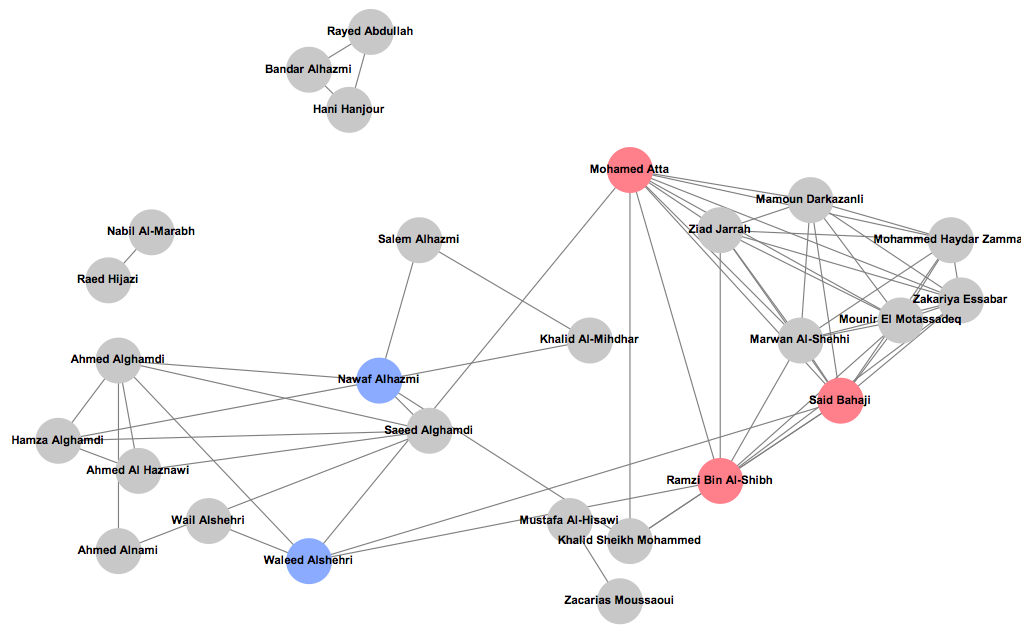
\includegraphics[scale=0.4]{imgs/T1999-01.png}
\end{center}
\caption{The 9/11 terrorist network in January 1999}
\end{figure}

\begin{figure}[h]
\label{Terrorist-Dec00}
\begin{center}
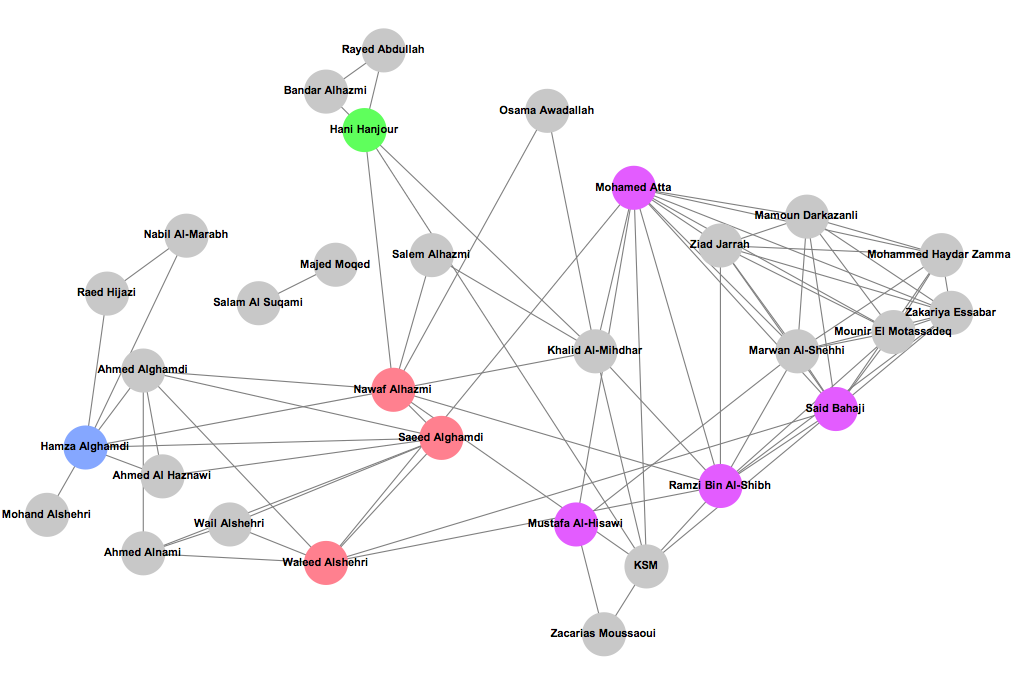
\includegraphics[scale=0.4]{imgs/T2000-12.png}
\end{center}
\caption{The 9/11 terrorist network in December 2000}
\end{figure}

\begin{figure}[h]
\label{Terrorist-May01}
\begin{center}
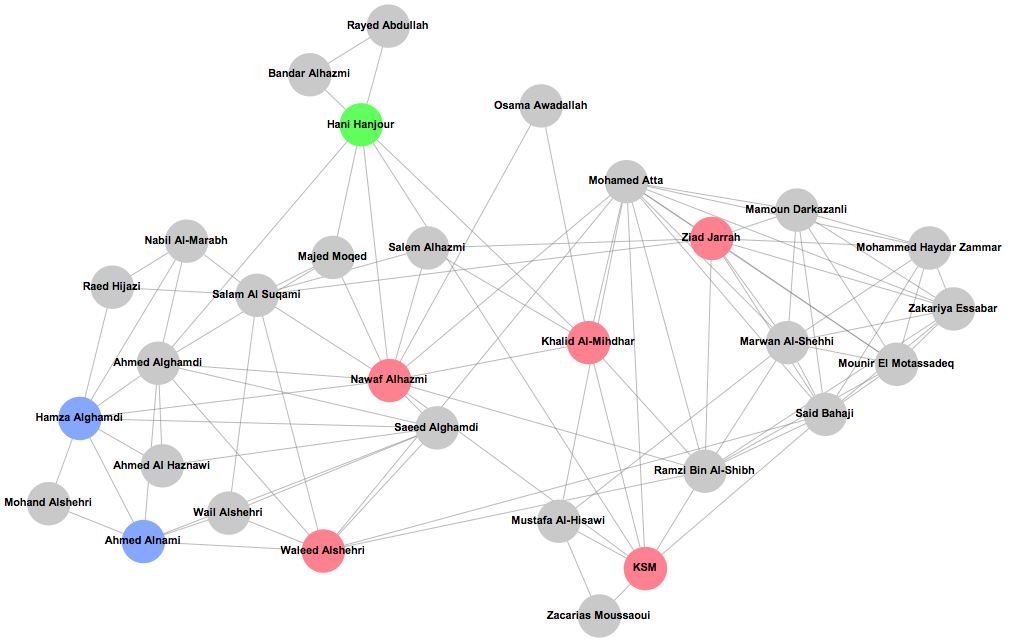
\includegraphics[scale=0.4]{imgs/T2001-05.png}
\end{center}
\caption{The 9/11 terrorist network in May 2001}
\end{figure}

\begin{figure}[h]
\label{Terrorist-Aug01}
\begin{center}
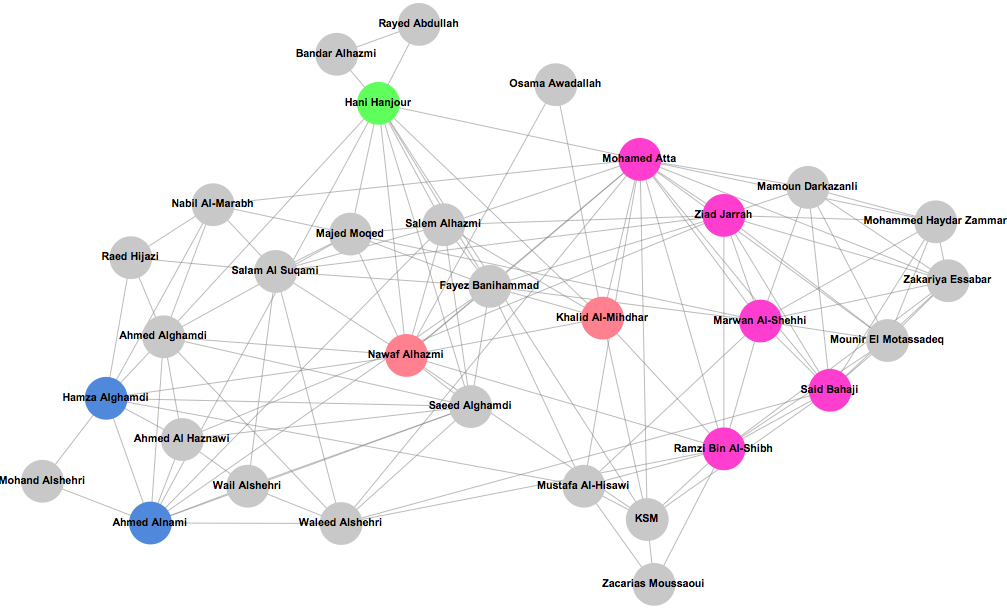
\includegraphics[scale=0.4]{imgs/T2001-08.png}
\end{center}
\caption{The 9/11 terrorist network in August 2001}
\end{figure}

\newpage

\begin{sidewaystable}[t]
\begin{center}
\begin{tabular}{l cc cccccccc}
\toprule
 & \multicolumn{2}{c}{Jan 1999} & \multicolumn{2}{c}{Dec 2000} & \multicolumn{2}{c}{May 2001} & \multicolumn{2}{c}{Aug 2001} & \multicolumn{2}{c}{Average} \\[1ex]
\midrule
Name  & $\overline{\beta}(i)$ & $\widetilde{\beta}(i)$ & $\overline{\beta}(i)$ & $\widetilde{\beta}(i)$ & $\overline{\beta}(i)$  & $\widetilde{\beta}(i)$ & $\overline{\beta}(i)$ & $\widetilde{\beta}(i)$ & $\overline{\beta}(i)$ & $\widetilde{\beta}(i)$ \\
\midrule
Ahmed Al-Haznawi       & 0.195     & 0.000       & 0.198     & 0.000       & 0.181     & 0.000        & 0.183     & 0.058       & 0.189            & 0.015             \\
Ahmed Alghamdi         & 0.388     & 0.422       & 0.224     & 0.323       & 0.221     & 0.508        & 0.185     & 0.237       & 0.255            & 0.373              \\
Ahmed Alnami           & 0.191     & 0.000       & 0.202     & 0.043       & 0.241     & 0.264        & 0.250     & 0.327       & 0.221            & 0.159              \\
Bandar Alhazmi         & 0.219     & 0.407       & 0.175     & 0.000       & 0.118     & 0.000        & 0.109     & 0.000       & 0.155            & 0.102              \\
Hamza Alghamdi         & 0.200     & 0.063       & 0.510     & 0.448       & 0.278     & 0.445        & 0.252     & 0.510       & 0.310            & 0.367             \\
Hani Hanjour           & 0.219     & 0.407       & 0.392     & 0.350       & 0.751     & 0.456        & 0.851     & 0.500       & 0.553            & 0.428            \\
Khalid Al-Mihdhar      & 0.172     & 0.000       & 0.254     & 0.273       & 0.244     & 0.406        & 0.250     & 0.230       & 0.230            & 0.227              \\
Mamoun Darkazanli      & 0.202     & 0.000       & 0.201     & 0.000       & 0.182     & 0.000        & 0.183     & 0.000       & 0.192            & 0.000               \\
Marwan Al-Shehhi       & 0.202     & 0.003       & 0.213     & 0.228       & 0.201     & 0.142        & 0.184     & 0.384       & 0.200            & 0.189            \\
Mohamed Atta           & 0.226     & 0.229       & 0.232     & 0.571       & 0.203     & 0.312        & 0.184     & 0.500       & 0.211            & 0.403            \\
Mounir El Motassadeq   & 0.202     & 0.003       & 0.201     & 0.011       & 0.182     & 0.008        & 0.183     & 0.023       & 0.192            & 0.011              \\
Mustafa Al-Hisawi      & 0.219     & 0.407       & 0.223     & 0.164       & 0.237     & 0.203        & 0.194     & 0.225       & 0.218            & 0.250              \\
Nabil Al-Marabh        & 0.219     & 0.407       & 0.175     & 0.000       & 0.189     & 0.102        & 0.185     & 0.180       & 0.192            & 0.172             \\
Nawaf Al-Hazmi         & 0.563     & 0.405       & 0.403     & 0.444       & 0.264     & 0.600        & 0.250     & 0.257       & 0.370            & 0.427            \\
Raed Hijazi            & 0.219     & 0.407       & 0.175     & 0.000       & 0.179     & 0.028        & 0.183     & 0.000       & 0.189            & 0.109              \\
Ramzi Bin Al-Shibh     & 0.226     & 0.226       & 0.225     & 0.500       & 0.186     & 0.214        & 0.195     & 0.515       & 0.208            & 0.364              \\
Rayed Abdullah         & 0.219     & 0.407       & 0.175     & 0.000       & 0.118     & 0.000        & 0.109     & 0.000       & 0.155            & 0.102              \\
Saeed Alghamdi         & 0.221     & 0.124       & 0.228     & 0.366       & 0.195     & 0.236        & 0.183     & 0.084       & 0.207            & 0.203            \\
Said Bahaji            & 0.226     & 0.229       & 0.215     & 0.312       & 0.185     & 0.168        & 0.184     & 0.221       & 0.203            & 0.233             \\
Salem Alhazmi          & 0.172     & 0.000       & 0.196     & 0.000       & 0.183     & 0.093        & 0.183     & 0.042       & 0.184            & 0.034             \\
Wail Alshehri          & 0.171     & 0.000       & 0.198     & 0.000       & 0.183     & 0.057        & 0.183     & 0.023       & 0.184            & 0.020             \\
Waleed Al-Shehri       & 0.492     & 0.439       & 0.346     & 0.288       & 0.205     & 0.264        & 0.183     & 0.163       & 0.307            & 0.289            \\
Zacarias Moussaoui     & 0.219     & 0.407       & 0.201     & 0.107       & 0.169     & 0.000        & 0.181     & 0.000       & 0.193            & 0.129             \\
Zakariya Essabar       & 0.202     & 0.003       & 0.201     & 0.011       & 0.182     & 0.008        & 0.183     & 0.023       & 0.192            & 0.011              \\
Ziad Jarrah            & 0.202     & 0.003       & 0.201     & 0.011       & 0.189     & 0.237        & 0.184     & 0.332       & 0.194            & 0.146              \\
KSM                    & 0.397     & 0.261       & 0.251     & 0.468       & 0.262     & 0.429        & 0.195     & 0.372       & 0.276            & 0.383             \\
Mohammed Haydar Zammar & 0.202     & 0.000       & 0.201     & 0.000       & 0.182     & 0.000        & 0.183     & 0.000       & 0.192            & 0.000               \\
Mohand Alshehri        & --        & --          & 0.000     & 0.000       & 0.171     & 0.000        & 0.170     & 0.000       & 0.085            & 0.000               \\
Satam Al-Suqami        & --        & --          & 0.000     & 0.000       & 0.232     & 0.578        & 0.185     & 0.271       & 0.104            & 0.212             \\
Majed Moqed            & --        & --          & 0.000     & 0.000       & 0.182     & 0.054        & 0.183     & 0.000       & 0.091            & 0.014               \\
Osama Awadallah        & --        & --          & 0.196     & 0.000       & 0.171     & 0.000        & 0.170     & 0.000       & 0.134            & 0.000               \\
Fayez Banihammad       & --        & --          & --        & --          & --        & --           & 0.183     & 0.099       & 0.046            & 0.025            \\
\bottomrule
\end{tabular}
\end{center}
\caption{Normalised brokerage and criticality results for all 9/11 terrorists across all observed time periods}
\label{allterrorists}
\end{sidewaystable}

\end{subappendices}
\part{Entrepreneurship in a Platform Economy} 
\label{part:entrepreneurshipPlatformEconomy}

\section*{Overview of Part III}

Out of the economic states discussed within the monograph, the Platform economy is the one most closely related to that of contemporary society. Within this economy hierarchical production organisations become more developed and sprawling structures such that platforms are created: hierarchical production organisations that exists in multiple aspects of the socio-economic space and facilitates interaction between agents within multiple aspects of the economy. The existence of platforms expresses the presence of more sprawling economic interactions between agents embedded in multiple aspects of the socio-economic space. Platforms can, therefore, facilitate economic interaction between aspects of the socio-economic space and, in doing so, can potentially broker these relations.

Part~\ref{part:entrepreneurshipPlatformEconomy} formally illustrates the notion of aspects and platforms---and the interaction between these notions---through the use of hypergraphs and hyperlinks. Empirically, we illustrate aspects, platforms, and entrepreneurship within this environment with an analysis of directorate networks. Of specific interest are the directorate networks of New York City during its development in the early 20th century.

\subsection*{Chapter breakdown}

This Part is comprised of two interlinked chapters. The first, \emph{Measuring control in hypergraphs}, provides a formal investigation into how aspects and platforms are considered in terms of hypergraphs, and how influence and positions of power can be identified and measured in a formal manner.

The second chapter, \emph{Control in the Platform economy: The case of New York City}, uses the theory and measures developed in the previous chapter. A specific application is on the assessmenet of the tangled directorate network within the financial, insurance, and railroad industries of New York City between 1902 and 1912. We show the evolving network of relationships and analyse how individuals and firms attained power within the network by forming relationships with other firms between multiple industries of the economy and, in doing so, bridging structural holes. Further, the final chapter investigates the relationship between the economic performance of a firm and the position of the firm within the directorate network. It is found that firms that orientate themselves to fill a structural hole will tend to have better economic performance. A specific example of this is the Banker's Trust.
\chapter{Measuring control in hypergraphs}

Hierarchical production organisations are often characterised by a distinction between ownership and control \citep{JensenMeckling1976, FamaJensen1983}. This separation leads to a distinction between the roles of `shareholders' and the `directors' within a firm. Shareholders and directors can own and control many firms across many different industries of the economy. As such, a set of firms can have \emph{overlapping} and \emph{interlocking} directorates depending on how their directors form memberships to multiple firms within the set. Note that we consider an overlapping directorate and an interlocking directorate as different notions. When a director sits on the boards of multiple firms we suggest that the directorates of these firms `overlap' due to the presence of at least one identical director. If firm $A$ has an overlapping directorate with firm $B$, and firm $B$ has an overlapping directorate with some other firm $C$ then we claim that firms $A$ and $C$ are `interlocked' due to their mutual overlap with firm $B$'s directorate. According to the definition of the interlocks during the time in which they were initially debated, the directorate of firms $A$ and $C$ need not overlap for there to be an interlock; it must simply be that directors from firm $A$ and firm $C$ be connected by some intermediary in which they both have a mutual overlap with.

The structure of interlocking and overlapping directorates has gained much interest in both industry and academia over the past century. This research has focused on the relationship between overlapping and interlocking directorates, the positional power of well-connected firms and directors, and the spread of corporate governance through sprawling directorate networks \citep{RoyBonacich1988}. The consequence of the research is a raft of accepted stylised facts and policy implications suggesting that tightly-knit directorate networks within an industry, and between related industries, is an uncompetitive practice. The epitome of this being the unbridled power of J.P. Morgan and his associates. This chapter uses novel methodology in network theory to test the stylised facts surrounding interlocking directorates during the height of Morgan's influence. Specifically, by using directorate data we elaborate on the actions of network entrepreneurship within a platform economy using the example of New York City at the beginning of the twentieth Century. We also feed the notion of network entrepreneurship into a discussion of institutional entrepreneurship by elaborating on how the capitalists at the time forced a change to the institutional design of American business. Furthermore, the chapter finds that whereas the number of interlocks are largely irrelevant for a firms performance, the weights and context of the interlocks matters significantly to the profitability of the firm.

\subsubsection{J.P. Morgan and the \emph{Money Trust}}

The structure and potential influence of directorate networks were brought to the fore within industry in 1912 when the United States House Committee on Financial Services organised a special committee---named the \emph{Pujo Committee}---to investigate a so-called `Money Trust'. This was seen to be a \emph{de facto} monopoly of control by a handful of financial institutions and bankers across multiple industries. Specifically, John Peirpont Morgan and his financial institution, J.P. Morgan \& Co., were accused of holding and exercising excessive economic power across the United States of America through directorial ties and shareholdings in other firms. The hearing concluded in 1913 and Morgan was found capable of exercising monopoly power over a number of industries---including the railway industry, the financial services industry and insurance---and exercising excessive bargaining power when writing contracts through his own shareholdings and board memberships, and the board memberships of his employees of J.P. Morgan \& Co \footnote{Evidence of the investigation can be found at \href{https://fraser.stlouisfed.org/title/?id=80}{https://fraser.stlouisfed.org/title/?id=80}.}.

The outcome of this investigation lead to the passing of the \emph{Federal Reserve Act of 1913} and the \emph{Clayton Antitrust Act of 1914}. The Federal Reserve Act immediately lead to the establishment of the Federal Reserve Central Bank; which had been discussed for several years prior to the investigation as a reaction to the panics of 1907 and 1911 \citep{Silber2007}. The Clayton Antitrust Act, built upon the Sherman Antitrust Act of 1890, was an effort to reduce monopolisation and other anti-competitive practices such as price discrimination, exclusive dealing agreements, tying agreements, and mergers and acquisitions that would reduce market competition. Title 15, Chapter 1, Section 19 of this Act concerned interlocking directorates and officers. It aimed to reduce the number of overlapping and thus interlocking directorates of competing firms within the same industry and across industries. Although the law was not strictly enforced, it gradually lead to a weakening of the American directorial elite throughout the early and mid twentieth Century \footnote{Note, however, that other social and economic phenomena occurred during this time which would dilute the power of directors, such as a developing stock market and social, economic, and financial globalisation}. This was indeed a pivotal time in financial and economic history throughout the developed world. These anticompetitive institutions were later adopted by other economies, including in the UK, where there had been a swathe of industrial mergers and acquisitions in the financial and railway industry. Undeniably Morgan, and those associated with him and his company, had some power over the economic success of others.

One of Morgan's known interests was the establishment of the Northern Securities Company in 1901
\citep{Langdell1903}. The company was a railroad trust specifically purchasing shares of other important railroad companies, such as the Burlington and Quincy Railroad, which was a vital railroad hub in Chicago. The reason for its establishment was in response to a bidding war between Hill, Morgan, and Edward H. Harriman, the then President of the Union Pacific Railroad, for the shares of Northern Pacific Railway, owned by Hill and Morgan. Subsequently this bidding war transferred into competition for the shares of Burlington and Quincy Railroad. Hill created the Northern Securities Company to control all three railroads. The company was established and capitalised at \$400 million, with James J. Hill serving as its President, who was also the President of the Great Northern Railway.

The establishment of the company was considered by the Department of Justice as being anti-competitive, specifically breaching the Sherman Antitrust Act of 1890. There were multiple reasons as to why the Northern Securities Company was seen to be anti-competitive: first, due to a \emph{de facto} monopolisation through merger from a harmonisation of incentives and cooperation between directors of multiple rival railway companies; second, diluting competition regarding the the purchasing of shares of other railroad companies; and third, it reduced the potential for new competitor railroads that could easily be subsumed by the Northern Securities Company. In 1904 the Department of Justice ruled five votes to four in favour of dissolving the Northern Securities Company. This was one of the first uses of the Sherman Act, and set the foundation for 44 other Federal Antitrust cases.

This was an important time in the development of the United States and the mentality surrounding mergers, monopolies, and overlapping directorates. However, in general, regulation was lax surrounding the structure of directorate networks. It is therefore interesting to see whether the structure of the directorate network is reflective of economically powerful and anti-competitive practices, and to develop measures in an effort to identify powerful and influential directors and firms.

\medskip\noindent This chapter follows on from the discussion of network and institutional entrepreneurship, and previous interest in the structure of directorate networks. We also research whether the control of a firms' directorate has an impact on its economic performance. To answer this we develop a bespoke measure---the $\sigma$-score---which regards the control of individual directors and firms. Moreover, we characterise elite directors and assess whether the presence of so-called \emph{elites} within a firm has an impact on its performance.

Two issues of identification and measurement are resolved in this chapter. The first pertains to the identification of nodes and affiliations that have control in a directorate network, which is represented in the most general context as a \emph{hypergraph}. A hypergraph is a generalisation of a network that contains a set of links and a set of nodes. In a hypergraph a link---called a \emph{hyperlink}---can connect to multiple nodes, suggesting that all nodes are connected with each other. This provides a good setting for defining boards of directors whereby a node represents an individual director and a hyperlink represents a firms. From this we test whether a firms control has causality on its economic performance. The second pertains to the identification of elites; nodes that are embedded in all aspects of a socio-economic space. Due to their multiplicity of embeddedness and their ability to directly gather and use diverse and complimentary information we assess whether the presence of elites organise the evolution of the directorship network over time. Whereas the $\sigma$-score is a degree-based centrality measure, and therefore increases in a strictly monotonic fashion with the degree of the node, the measure of elites is not.

The process of parsing out sets of elites uncovers an \emph{elite network structure} whereby elites are connected through all aspects of the network. From the resulting elite network structure we assess elite power through brokerage measures and identify important subsets of nodes who hold controlling positions within elite structures, possessing some hierarchy over the set of elites. Using this information regarding the elites and influence of individual nodes and affiliations we use this information as inputs for a regression analysis that measures whether these factors have an impact on the value of a firms assets. There are a number of derived questions, such as whether the influence and connectivity of a financial institution has an impact on their lending, borrowing, and stability over time.

In this chapter we further argue that networks regarding firm directorships lend themselves to a multidimensional analysis. In such networks we consider a dimension to be equivalent to a specific industry of an economy. How related dimensions are measured by the nodes embedded within them and the consistency of the linkages between the nodes. Power between dimensions is therefore held by nodes that have access to information between them.

\paragraph{Chapter outline.}

First, we provide a literature review on the interaction between how connected directorates are within firm boards and the firms performance. Section~\ref{Theory:Influence} introduces hypergraphs, networks, and other preliminary concepts. The section then provides some bespoke ways in which to measure the influence of individual nodes and affiliations in hypergraphs and network projections. Section~\ref{Theory:Elites} introduces aspectual hypergraphs, analyses and provides measures for the relatedness between aspects, and finally defines elites and elite structures.

\section{Corporate connectivity and firm performance} \label{Literature}

Economics and sociology have investigated the relationship between an individuals' social structure and their economic outcomes \citep{Granovetter1985}. This literature includes analysis into the diffusion and adoption of innovation \citep{Coleman1966}, coalition formation \citep{Kapferer1969}, elite decision making and community structure \citep{LaumannGalaskiewiczMarsden1978}, information diffusion in labor markets \citep{Granovetter1973}, and decisions regarding the level of education that an individual pursues and whether or not to undertake criminal activity \citep{BallesterZenou2006, Jackson2007}. The types of networks examined in these papers include social communities, powerful families and political and economic systems \citep{Padgett1993, Padgett1994}. More recently, \citet{Banerjee2013} discussed the social structure regarding the diffusion of micro-finance practices that depends on the structure of society.

%%

There have been numerous studies on the social structure produced by members of boards of directors. For example, \citet{Levine1972} documents the existence of interlocked directorates between the boards of major banks and the boards of major industrials. Related to our study, \citet{Dooley1969} observes that an industrial company whose board is occupied by a banker can obtain capital at favourable rates. Much of this prior research documents how particular interlocks are created \citep{PfefferSalancik1978}, how they are maintained \citep{Palmer1983, PalmerFriedlandSingh1986}, the density or centrality of the network \citep{DavisYooBaker2003}, and the stability of the network though time \citep{BeckmanHaunschildPhillips2004}. However, relatively little work documents the economic consequences of these board networks on firm performance.

The association between a firm's centrality, connectedness, or importance in the interlocking boardroom network is ex-ante theoretically ambiguous. There is an abundance of arguments within organisational sociology and economics on why companies with well-connected boards may benefit from their position in the network. First, interlocking boardroom networks allow firms to improve the terms of contracts between firms \citep{SchoormanBazermanAtkin1981}. Second, because directors have important knowledge and contacts, being central in the boardroom network gives a firm better access to such useful knowledge, contacts and resources, which can benefit firms and particularly those that operate in uncertain business environments \citep{Mol2001, NicholsonAlexanderKiel2004}. Third, being central in the interlocking boardroom network could also allow for more or better means of information exchange, leading to a reduction in the costs of obtaining information and perhaps improving business decisions \citep{Mizruchi1990}. Fourth, board connections also represent a mechanism through which value-improving business innovations can spread in this way, being central in a network can add value to a firm \citep{HaunschildBeckman1998}. Finally, interlocking boardroom networks may facilitate cartel formation, which can yield private economic benefits within the cartel by restricting competition.

However, there are also plausible reasons why connectedness in the board network can negatively impact a firm. First, the extent that being well-connected in the boardroom network involves having boardroom members that take on many boardroom jobs, a firm may suffer economically from the deteriorating quality if their directors work in the firm \citep{FichShivdasani2006, FichWhite2005}. Second, it is possible that misleading or incorrect information is spread though the board network. The problems of misinformation are heightened with more sprawling interlock networks. If this information is used for strategic choices, it can easily result in a decrease in shareholder value. Finally, although collusion can have a positive impact on shareholder value, the resulting regulatory, litigation, and reputation costs can produce substantial losses of shareholder value.

This chapter is related to an emerging body of literature in economics, finance, and sociology demonstrating the role of personal and social connections in the spread of information. The chapter also contributes to the literature providing a link between social networks and favourable economic outcomes. For example, \citet{HwangKim2009} and \citet{HwangKim2012} demonstrate that socially connected CEO's enjoy higher compensation and retention rates; \citet{FaccioMcConnellMasulis2006} establish that politically connected firms have a higher likelihood of receiving bailout assistance; and \citet{StuartYim2010} find that connected firms have a higher propensity to be targeted in mergers and acquisitions deals. Our findings corroborate and extend this literature by providing additional evidence of the influence of social networks on firm-level economic outcomes. Specifically, our results suggest that firms central in the broader interlocking boardroom network experience improved operating and stock price performance.

Some prior research has delved into similar empirical questions. \citet{EngelbergGaoParsons2013} demonstrates that firms with connections to capital suppliers enjoy more favourable terms of lending, improved credit ratings, and superior stock price performance. \citet{Boyd1990} finds that among firms facing a more uncertain business environment, those with more connections to other companies through interlocks tend to perform better in terms of sales improvements and return on equity. Using a sample of 350 Brazilian firms, \citet{SantosSilveiraBarros2009} find that firm value is negatively affected by interlocking boards, particularly boards with busy boards and firms in which CEO's hold directorships in other companies. 

% Similarly, \citet{NonFrances2007} find a negative relationship between the number of interlocks and future performance for a sample of 101 Dutch firms.

These past studies are important. However, we suggest that there is a limitation to using standard centrality measures when applying them to specific environments such as boards of directors. Indeed, the outcomes witnessed from using off-the-shelf measures may be different from alternative, purpose-built centrality measures. In this chapter we provide a measure of a nodes influence, which we argue can be appropriately applied to directorate networks; this is extended to find the influence of firms to which the directors are members of. Of interest is the importance and influence of elites: directors who have influence in multiple industries.

% De Long (1990) finds that J.P. Morgan and Co., and those organisations associated with Morgan and his men, benefited from persistent economic benefits in the form of around a $30\%$ increase in common stock equity value. Ramirez (1995) further finds that organisations associated with Morgan benefited from decreased liquidity constraints. Chernow (2010) chronicles the rise of the House of Morgan, elaborating on J.P. Morgan's ability to monopolise lending and forming de facto oligopolies within the railway industry.

%\subsection{Measures of centrality}

%Freeman (1977) and Bonahich (1972) were first to develop measures of network centrality that are still commonly used network science \footnote{For more information on commonly used node centrality measures consider Jackson (2008).}. The degree and eigenvector centrality measures provide the foundation for other centrality measures that have been subsequently developed. The most common, the degree centrality, is determined by the number of links a given node has, and the eigenvector centrality measure is determined by the number of links that a node has and the number of links that each of its neighbours have. PageRank centrality (Brin and Page, 1998) develops a measure that is built from eigenvector centrality; it specifically discounts the importance of a nodes link by the number of other connections the node has. These common measures of centrality have been applied to many different social and economic contexts, and have had application to directorate networks (Khanna et al., 2015; El-Khatib, 2015). Sims and Gilles (2014) provide a measure brokerage attached to a node set, which is related to the economic notion of contestability.

%Of specific interest to this chapter is the work of Brink and Gilles (1996; 2000). The authors develop a measure of node dominance, known as the $\beta$-measure, which provides an axiomatic generalisation of degree centrality in a directed network. The measure has had specific application to tournaments and games, but has yet to be applied to directorate networks. Borm, Brink, and Slikker (2002) develop an iterated $\beta$-measure which, much like the eigenvector and PageRank centralities, develops a score based on the dominance of the nodes that it dominates. Again, this lacks a specific application to directorate networks.

%When considering directorate networks, the analysis of how industries are connected through a directorate is important. It can reveal complementaries and information sharing between industries unobservable by assessing outputs alone. A directors ability to have influence and share information between industries can reveal some importance. Corominas-Murtra and Thurner (2014) develop a mechanism in which to identify the weak core and the structure of important nodes within a multidimensional network. Nodes that exist within a $k$-core and within multiple dimensions of the network are termed as elites: these elites will exist within a so-called \emph{rich club} (Colizza et al., 2006).

\section{Centrality and influence in hypergraphs} 
\label{Theory:Influence}

Of specific interest to this chapter is the work of \citet{BrinkGilles1996, BrinkGilles2000}. The authors develop a measure of node dominance, known as the $\beta$-measure, which provides an axiomatic generalisation of degree centrality in a directed network. The measure has had specific application to tournaments and games, but has yet to be applied to directorate networks. \citet{BormBrink2002} develop an iterated $\beta$-measure which, much like the eigenvector and PageRank centralities, develops a score based on the dominance of the nodes that it dominates. Again, this lacks a specific application to directorate networks.

When considering directorate networks, the analysis of how industries are connected through a directorate is important. It can reveal complementaries and information sharing between industries unobservable by assessing outputs alone. A directors ability to have influence and share information between industries can reveal some importance. \citet{Corominas-MurtraThurner2014} develop a mechanism in which to identify the weak core and the structure of important nodes within a multidimensional network. Nodes that exist within a $k$-core and within multiple dimensions of the network are termed as elites: these elites will exist within a so-called \emph{rich club} \citep{Colizza2006}.

We construct a number of measures that compute the control of individual nodes and affiliations; particularly in the format of interlocking directorates. To do this we first introduce need to introduce some preliminary concepts, such as hypergraphs and its projections. From this we can investigate degree-based centrality measures, and extend these to incorporate the influence of individuals and affiliations. This provides the structure for this section.

\subsection{Preliminaries}

\subsubsection*{Hypergraphs}

Let $N = \{ 1, \ldots ,n \}$ be a finite set of \emph{nodes}. In this case, a node represents a director who serves on the board of one or more firms.

An \emph{affiliation} is any subset $H \subset N$ of nodes. Technically, an affiliation is defined as a hyperlink on node set $N$. In the case that we are interested in here an affiliation $H$ represents the board of directors of some firm.

A hypergraph is a node set endowed with a set of affiliations. Formally, a \emph{hypergraph} is now a pair $(N, \Gamma )$, where
\begin{equation}
\Gamma \subset \{ H \mid H \subset N \mbox{ and } H \neq \varnothing \} \equiv 2^N \setminus \{\varnothing\} ,
\end{equation}
and $| \Gamma | = h$ where $| \Gamma |$ denotes the number of elements in the finite set $\Gamma$.

A hypergraph thus represents an affiliation situation in which individuals, represented as nodes, are organised into affiliations, represented by hyperlinks. Usually we will use the shorthand notation $\Gamma$ as the hypergraph or affiliation situation where the node set $N$ is unambiguous.

We can formally define an ``affiliation situation'' as the class of all hypergraphs, $\mathbb{H}$, as
\begin{equation}
\mathbb{H}^N = \{ \Gamma \mid \Gamma \subset 2^N \mbox{ is an affiliation situation on } N \} .
\end{equation}

\paragraph{Neighbourhoods.}

Let $\Gamma \subset 2^N$ be some hypergraph. Then the \emph{affiliation set} of $i \in N$ is defined by
\begin{equation}
\Gamma_i = \{ H \in \Gamma \mid i \in H \}
\end{equation}
Thus, the affiliation set of a node is simply the collection of affiliations that it is a member of. This naturally leads to the identification of all nodes or individuals that a node encounters in its affiliations. The \emph{neighbourhood} of a node $i \in N$ is defined by
\begin{equation}
\overline{\Gamma}_i = \cup \Gamma_i \setminus \{ i \}
\end{equation}
The neighbourhood of a node is the set of nodes that are members of the affiliations that the node is involved with.

\paragraph{Overlapping affiliations.}

We allow that individual nodes can participate in multiple affiliations. The outcome is the overlap of multiple affiliations through a set of mutual nodes. It is clear that a set of affiliations, $\mathcal{H} \subseteq \Gamma$, are \emph{overlapping} if
\begin{equation}
\bigcap_{H \in \mathcal{H}} H \neq \varnothing .
\end{equation}
The \emph{environment} of $H \in \Gamma$, denoted by $\mathcal{E}_{H}$, is given as
\begin{equation}
\mathcal{E}_{H} = \{K \in \Gamma \, \mid \, K \cap H \neq \varnothing \mbox{ and } K \neq H \} .
\end{equation}
$\mathcal{E}_{H}$ is the largest set of overlapping affiliations containing $H$.

\paragraph{Weighted hypergraph.}

A hypergraph structure can be generalised by adding a weight to each affiliation; the result of which is a \emph{weighted hypergraph}, denoted by $\Gamma'$, in which the weight of some $H \in \Gamma$ is given by some real number which is denoted by $\nu_{H} \in \mathbb{R}$. A weighted hypergraph is therefore defined by the triple $\Gamma' = (N, \Gamma, \mathbf{v})$ where $N$ and $\Gamma$ are the set of nodes and affiliations respectively, as defined above, and $\mathbf{v} = (\nu_{1}, \ldots , \nu_{h})$ is a vector of weights that are attached to each affiliation.

Much like above, we can define a `weighted affiliation situation' as:
\begin{equation*}
\mathbb{L}^N = \{ \Gamma' \mid \Gamma' \subset 2^N \times \mathbf{v} \mbox{ is a weighted affiliation situation on } N \} ,
\end{equation*}
The weight of an affiliation can refer to the intensity of the relationship between its members, such that a larger weight denotes a greater intensity. Within our context, however, the weight of the affiliation specifically denotes the ``economic value'' of the affiliation. More specifically, as discussed in the application below, the weight of a firm refers to the value of the firms' total assets.

\begin{figure}[t]
\begin{center}
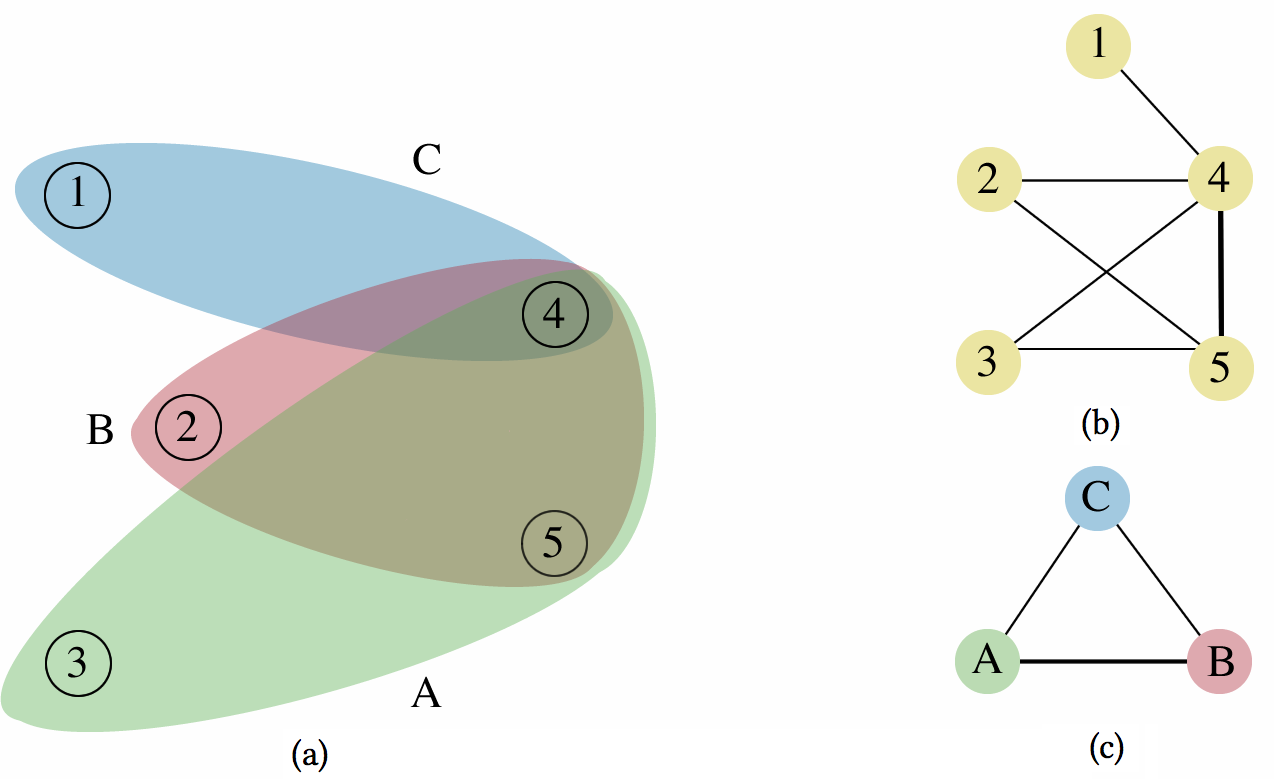
\includegraphics[scale=0.28]{imgs/hypergraph.png}
\end{center}
\caption[Hypergraph and network projections]{Figure (a) is a hypergraph containing five nodes and three affiliations. Network (b) is the affiliation projection of hypergraph (a). Network (c) is the node projection of hypergraph (a).}
\label{hypergraph}
\end{figure}

\subsubsection*{Networks}

A hypergraph can be projected into two networks: the first is a \emph{node projection} and the second is an \emph{affiliation projection}. The projections are represented as networks and therefore we use the term `network' and `projection' interchangeably. These projections are useful for assessing overlapping and interlocking directorates of firms, which will be assessed throughout the chapter.

\paragraph{Node projection.}

A hypergraph can be projected on the node set $N$. A node projection of the hypergraph $\Gamma$ is denoted by $g_N$, which refers to the set of relationships $g_N = \{ij \, \mid \, j \in \overline{\Gamma}_{i} \mbox{ and } i \neq j \}$, where $ij$ is an \emph{undirected link} between nodes $i$ and $j$, such that $ij = ji$, therefore if $ij \in g_{N}$ then $ji \in g_{N}$. The node network from the hypergraph in Figure~\ref{hypergraph} (a) can be seen in Figure~\ref{hypergraph} (b).

\paragraph{Affiliation projection.}

Furthermore, a hypergraph can be projected into an affiliation projection on the set of affiliations, $\Gamma$. An affiliation network of the hypergraph $\Gamma$ is denoted by $G_{\Gamma}$, which refers to a set of reciprocated \emph{arcs} $G_{\Gamma} = \{ HK \, \mid \, K \in \mathcal{E}_{H} \mbox{ and } H \in \Gamma \}$. The affiliation network from the hypergraph in Figure~\ref{hypergraph} (a) can be seen in Figure~\ref{hypergraph} (c).

The links between the nodes the in the node projection of a hypergraph can have a weight determined by the number of mutual affiliations between the nodes. Moreover, the arcs in the affiliation projection can have a weight determined by the number of mutual nodes between the affiliations. Formally, with respect to the node projection, the weight on an a link between a pair of nodes $i,j \in N$ is given by
\begin{equation} \label{eq:nodeweight}
\omega_{ij}(\Gamma) = | \overline{\Gamma}_{i} \cap \overline{\Gamma}_{j} | .
\end{equation}
Also, with respect to the affiliation projection, the weight on an arc from affiliation $H \in \Gamma$ to another affiliation $K \in \Gamma$ is given by
\begin{equation} \label{eq:affweight}
\omega_{HK}(\Gamma) = | H \cap K | .
\end{equation}
If $\omega_{ij}(g_{N}) = 0$ then there does not exist a weighted undirected link between nodes $i$ and $j$. Likewise, if $\omega_{HK}(G_{\Gamma}) = 0$ then there exists no weighted arc from $H$ to $K$.

\subsection{Degree-based centrality measures in affiliation situations} 
\label{degreecentralities}

We provide a centrality measure for nodes and affiliations within the context of a hypergraph to be used in the analysis of empirical situations. The measure is directly related to the dependence of the affiliation on the individual node and the value of the affiliation(s) that the node is a member of. We use this to measure the influence of individual nodes and affiliations within a hypergraph.

Within this chapter we define `influence' as the ability for agents to control resources; which has particular importance with regard to directorate hypergraphs whereby the influence of a director is given by the voting rights of the director and the size of the firm(s) that they are members of. Indeed, having proportionally more voting rights to the decisions of a firm and/or being a board member of a highly valued firm will increase a directors influence on the resources that the firm owns. From this we can derive the external influence of an affiliation or firm, which refers to the total amount of resources that it can potentially control beyond itself. We define the influence of an individual or affiliation---given by the $\sigma$-score---in its most general form as a centrality measure on a hypergraph.
\begin{definition}
Let $N = \{ 1, \ldots ,n \}$ be a given set of nodes. A \textbf{centrality measure} on $N$ is a function $\varphi \colon N \times \mathbb{H}^N \to \mathbb{R}^N$.
\end{definition}
A centrality measure on $N$ is a function that for every affiliation situation represented by a hypergraph $\Gamma \subset 2^N$ assigns to every individual node $i \in N$ a real number $\varphi_i ( \Gamma )$ representing the importance of $i$ in $\Gamma$. Ideally the measure should correctly represent the importance of an individual in the corporate situation represented by $\Gamma$.

There exists no specific measure of centrality for hypergraphs; most measures are either derived from the degree of the node or derived from the paths and walks that a node lies on. We specifically focus on degree-based measures, elaborating on the standard degree measure, the generalised $\beta$-measure, and influence.

\subsubsection*{Standard degree measure}

The \emph{standard degree measure} is the centrality measure $\delta \colon N \times \mathbb{H}^N \to \mathbb{R}^N$, which for every node $i \in N$ is defined by
\begin{equation}
\delta_i (\Gamma ) = \left| \overline{\Gamma}_i \right| .
\end{equation}
For general hypergraphs the sum of the standard degree across all nodes is computed as
\begin{equation}
\sum_{i \in N} \delta_i (\Gamma ) = \sum_{H \in \Gamma} | H | \, ( \, | H | - 1) - \sum_{H,H' \in \Gamma} | H \cap H' | \cdot \frac{| H \cap H' | - 1}{2} .
\end{equation}
For hypergraphs where $| H | = 2$ for all $H \in \Gamma$, this simplifies to $\sum_{i \in N} \delta_i (\Gamma ) = \sum_{H \in \Gamma} | H | \, ( \, | H | - 1) = 2 \, | \Gamma |$. These are networks.

If $\Gamma$ is projected as a node network, $g_N$, the standard degree measure simplifies to the standard degree concept defined and used in network analysis given by
\begin{equation}
\delta_i (\Gamma ) = d_i (g_N ) = | \, \{ j \in N \mid \, j  \in \Gamma_{i} \mbox{ where } j \neq i \}  \, |.
\end{equation}
Likewise, for node projected hypergraphs where $| H | = 2$ for all $H \in \Gamma$ in the initial hypergraph, $\sum_{i \in N} d_i (g_{N}) = 2 \, | \Gamma |$.

Finally, we denote the degree of an affiliation, $H \in \Gamma$, in the affiliation projection of $\Gamma$ as $\delta_{H}(G_{\Gamma}) = | \mathcal{E}_{H} |$, or simply as $\delta_{H}$.

\subsection{A hypergraph $\beta$-measure}

The \emph{hypergraph} $\beta$-\emph{measure} is the centrality measure $\beta \colon N \times \mathbb{H}^N \to \mathbb{R}^N$ given by
\begin{equation}
\beta_i (\Gamma ) = \sum_{j \in \overline{\Gamma}_i} \frac{1}{\left| \, \overline{\Gamma}_j \right|}
\end{equation}
In the case that $\Gamma$ is a network on $N$ this simplifies to
\begin{equation}
\beta_i (g_{N}) = \sum_{j \in \overline{\Gamma}_i} \frac{1}{d_j (\Gamma )} \equiv \beta_i (\Gamma ) .
\end{equation}
which is indeed equivalent to the original formulation of the $\beta$-measure for networks by van den Brink and Gilles (1994). The $\beta$-measure is a measure of dominance whereby some node, $i$, dominates another, $j$, if $ij \in g_{N}$ or $\Gamma_{i} \cap \Gamma_{j} \neq \varnothing$. The total dominance distributed across the node set of the hypergraph is given by the total number of nodes that participate in at least one affiliation. We note this formally as
\begin{equation}
\sum_{i \in N} \beta_{i}(\Gamma) = | ~ \{ i \in N ~ | ~ \Gamma_{i} \neq \varnothing \} ~ | .
\end{equation}
The standard $\beta$-measure can be supported as a Shapley value of a corresponding TU-game describing the power relations in an affiliation situation.\footnote{A \textbf{TU-game} or ``cooperative game with transferable utilities'' on the node set $N$ is a function $v \colon 2^N \to \mathbb{R}$ such that $v( \varnothing )=0$. It describes the values that can be generated by groups of nodes in the affiliation situation under consideration. The \emph{Shapley value} of a TU-game $v$ is defined as $\phi_i (v) = \sum_{S \colon i \in S} \frac{\Delta_v (S)}{|S|}$, where $\Delta_v (S) = \sum{T \subset S} (-1)^{|S|-|T|} v(T)$ is the \emph{Harsanyi dividend} of the coalition $S$ in the game $v$.}
\begin{theorem}
Let $\Gamma$ be some affiliation situation on node set $N$. We define $V_{\Gamma} \colon 2^N \to \mathbb{R}$ as the TU-game given by
\begin{equation}
v_{\Gamma} (S) = \left| \, \cup_{j \in S} \overline{\Gamma}_j \, \right| .
\end{equation}
Then the Shapley value of $V_{\Gamma}$ coincides with the $\beta$-measure for $\Gamma \colon$
\begin{equation}
\phi_i \left( V_{\Gamma} \right) = \beta_i (\Gamma ) .
\end{equation}
\end{theorem}
\begin{proof}
This proof follows the outline of the proof of a corresponding result for the $\beta$-measure for networks given in Gilles (2010).
\\
Let $\Gamma \subset 2^N$ be some affiliation situation on $N$. For every node $i \in N$ we define a TU-game $w_i \colon 2^N \to \mathbb{R}$ by
\begin{equation}
w_i (S) = \left\{
\begin{array}{ll}
1 & \mbox{if } S \cap \overline{\Gamma}_i \neq \varnothing \\
0 & \mbox{otherwise}
\end{array} \right. .
\end{equation}
Then it is clear that for every $S \subset N$
\begin{equation}
V_{\Gamma} (S) = \sum_{i \in N} w_i (S) \quad \mbox{or} \quad V_{\Gamma} = \sum_{i \in N} w_i
\end{equation}
and, therefore, by additivity of the Shapley value it holds that for every $j \in N \colon$
\begin{equation}
\phi_j \left( V_{\Gamma} \right) = \sum_{i \in N} \phi_j \left( w_i \right) .
\end{equation}
We can determine that the Harsanyi dividends for $w_i$ are given by $\Delta_{w_i} (S) = (-1)^{|S|+1}$. Therefore,
\begin{equation}
\phi_j (w_i) = \sum_{S \subset N \colon j \in S} \frac{\Delta_{w_i} (S)}{|S|} = \sum_{S \subset \overline{\Gamma}_i \colon j \in S} \frac{(-1)^{|S|+1}}{|S|} .
\end{equation}
Hence, for every $j \in N \colon$
\begin{align*}
\phi_j \left( V_{\Gamma} \right) & = \sum_{i \in N} \phi_j (w_i) = \sum_{i \in N} \, \sum_{S \subset \overline{\Gamma}_i \colon j \in S} \frac{(-1)^{|S|+1}}{|S|} \\[1ex]
& = \sum_{i \in \overline{\Gamma}_j} \, \sum_{S \subset \overline{\Gamma}_i \setminus \{ i \} } \frac{(-1)^{|S|}}{|S|+1} \\[1ex]
& = \sum_{i \in \overline{\Gamma}_j} \, \sum^{D_i-1}_{t=0} \binom{D_i-1}{t} \, \frac{(-1)^t}{t+1}
\end{align*}
where we use the shorthand $D_i = \left| \overline{\Gamma}_i \right|$. Now,
\begin{align*}
\sum^{D_i-1}_{t=0} \binom{D_i-1}{t} \, \frac{(-1)^t}{t+1} & = \frac{-1}{D_i} \, \left[ \, \sum^{D_i}_{t=1} \binom{D_i}{t} \cdot (-1)^t \, \right] = \\[1ex]
& = \frac{-1}{D_i} \, \left[ \, \sum^{D_i}_{t=0} \binom{D_i}{t} \cdot (-1)^t -1 \, \right] = \\[1ex]
& = \frac{-1}{D_i} \, \left[ \, (1-1)^{D_i} -1 \, \right] = \frac{1}{D_i} .
\end{align*}
Therefore,
\[
\phi_j \left( V_{\Gamma} \right) = \sum_{i \in \overline{\Gamma}_j} \frac{1}{D_i} = \sum_{i \in \overline{\Gamma}_j} \frac{1}{\left| \overline{\Gamma}_i \right|} = \beta_j (\Gamma )
\]
This shows the assertion.
\end{proof}

\paragraph{Generalised $\beta$-measure.}

The $\beta$-measure can be generalised such that there can exist weights on the relations between the nodes. This is for specific application to weighted directed or undirected networks, however we can derive the $\beta$-scores of nodes given that there can exist weighted relations between nodes in the node projection of the hypergraph.

Let $\Gamma$ be a hypergraph on node set $N$, where $i,j \in N$, the \emph{generalised $\beta$-measure}, denoted by $\beta^{\star}_{i}(\Gamma)$ for some node $i$, is given by
\begin{equation}
\beta^{\star}_{i}(\Gamma) = \sum_{j \in \overline{\Gamma}_{i}} \frac{\omega_{ij}(g_{N})}{W_{j}(\Gamma)} ,
\end{equation}
where $\omega_{ij}(g_{N}) = | \Gamma_{i} \cap \Gamma_{j} |$, as in Equation~\ref{eq:nodeweight}, and $W_{i}(\Gamma) = \sum_{i \in \overline{\Gamma}_{j}} \omega_{ij}(\Gamma)$. The generalised $\beta$-measure distributes the dominance weight of a node proportional to the weights of the relations on which node $j$ is dominated. These weights emerge, as noted above, in the node projection of the hypergraph. A non-weighted network is equivalent to the weighted network with
\[
\omega_{ij}(g_{N} ) = \left\{
\begin{array}{ll}
1 & \mbox{if } \Gamma_{i} \cap \Gamma_{j}  \\
0 & \mbox{otherwise .}
\end{array} \right.
\]
But then $W_{j}(\Gamma) = d_{j}(\Gamma)$ for all $j \in N$ and $\omega_{ij}(\Gamma) = \omega_{ij}(g) \in \{0,1\}$, so $\beta^{\star}_{i}(\Gamma) = \beta_{i}(\Gamma)$. Thus, the generalised $\beta$-measure is indeed a generalisation of the $\beta$-measure.

With respect to the set of affiliations, we can measure their $\beta$-score in much the same way as with the generalised $\beta$-measure for the node set. Let $\Gamma$ be a hypergraph where $H, K \in \Gamma$ are affiliations and let
\begin{equation}
W_{K}(\Gamma) = \sum_{H \in \mathcal{E}_{K}} \omega_{HK}(G_{\Gamma}) ,
\end{equation}
where $\omega_{HK}(G_{\Gamma})$ is given by Equation~\ref{eq:affweight}. The generalised $\beta$-measure for affiliations is now given by
\begin{equation}
\beta^{\star}_{H}(\Gamma) = \sum_{K \in \mathcal{E}_{H}} \frac{\omega_{HK}(G_{\Gamma})}{W_{K}(\Gamma)} .
\end{equation}
Much like above, this leads to the property that $\sum_{H \in \Gamma} \beta^{\star}_{H} (\Gamma) = | ~ \{ H \in \Gamma ~ | ~ H \neq \varnothing \} ~ |$.

\paragraph{Axiomatisation of the generalised $\beta$-measure.}

The generalised $\beta$-measure can be characterised through the use of four axioms. We present these axioms on an arbitrary relational power measure $f : \mathbb{H}^{N} \rightarrow \mathbb{R}^{N}$, where any hypergraph structure, $\Gamma$, can be drawn from $\mathbb{H}^{N}$, that uniquely determine the generalised $\beta$-measure. These axioms are as follows.

\begin{axiom}[Weighted dominance normalisation] \label{ax:1}
For every $\Gamma \in \mathbb{H}^{N}$ it holds that
\[
\sum_{i \in N} f_{i}(\omega) = | ~ \{ j \in N ~ | ~ \lambda_{\omega}(j) > 0 \} ~ |
\]
\end{axiom}

\begin{axiom}[Weighted dummy node property] \label{ax:2}
For every $\Gamma \in \mathbb{H}^{N}$ and every $i \in N$ with $\Gamma_{i} = \varnothing$ it holds that $f_{i}(\omega) = 0$.
\end{axiom}

\begin{axiom}[Weight proportionality] \label{ax:3}
For every $\Gamma \in \mathbb{H}^{N}$ and every pair $i,j \in N$ for which there is a constant $c_{i,j} \in \mathbb{R}$ such that $\omega(i,h) = c_{i,j} \cdot \omega(j,h)$ for every $h \in N$ it holds that
\begin{equation}
f_{i}(\omega) = c_{i,j} \cdot f_{j}(\omega) ~ .
\end{equation}
\end{axiom}

To state the fourth axiom we introduce a partition of a hypergraph $\Gamma$ as a collection of hypergraphs $\mathcal{G} = \{\Gamma_{1}, \ldots, \Gamma_{m}\}$ such that $\sum_{\ell = 1}^{m} \omega_{ij}^{\ell} = \omega_{ij}$ for every $ij \in g_{N}$.


\begin{axiom}[Additivity over weighted independent partitions] \label{ax:4}
For every $\Gamma \in \mathbb{H}^{N}$ and independent partition $\mathcal{G}$ of $\Gamma$ it holds that
\begin{equation}
f(\omega) = \sum_{\omega_{k} \in \mathcal{G}} f(\omega_{k})
\end{equation}
\end{axiom}

The generalised $\beta$-measure satisfies these four axioms.

\subsection{A standard $\sigma$-score}

An alternative centrality measure is the \emph{$\sigma$-score} defined as the centrality measure $\sigma \colon N \times \mathbb{H}^N \to \mathbb{R}^N$ with for every node $i \in N \colon$
\begin{equation}
\sigma_i (\Gamma ) = \sum_{H \in \Gamma_i} \frac{1}{|H|}
\end{equation}
\begin{proposition} \label{prop:SG-degree}
Let $\Gamma$ be a hypergraph. If $| H | = 2$ for all $H \in \Gamma$, the $\sigma$-score becomes
\begin{equation}
\sigma_i (\Gamma ) = \tfrac{1}{2} \delta_i ( \Gamma ) ,
\end{equation}
meaning that $\sigma_{i}(G_{\Gamma}) = \tfrac{1}{2} d_{i} (G_{\Gamma})$ in the affiliation projection.
\end{proposition}
Due to Proposition~\ref{prop:SG-degree} the $\sigma$-score is to be viewed as a degree-based measure. In fact, in comparison with the standard degree measure, it is an alternative generalisation of the degree concept used in network analysis to the realm of hypergraphs or affiliation situations. Further still, we will show that the \emph{weighted $\sigma$-score} is a further generalisation of the generalised $\beta$-measure.

The normalisation of the $\sigma$-score on the node set $N$ of general hypergraphs is different from the normalisation of the degree measure and the $\beta$-measure. This normalisation is given by
\begin{equation} \label{eq:sigmanorm}
\sigma_{N} = \sum_{i \in N} \sigma_i (\Gamma ) = | \Gamma | .
\end{equation}
Equation~\ref{eq:sigmanorm} clearly indicates that the $\sigma$-score is a normalised degree measure that normalises to the number of affiliations in hypergraph $\Gamma$.

Regardless of both measures being degree-based Example~\ref{comparedegree} shows that different centrality measures can provide substantially different outcomes of relative node centrality. Specifically we note that the relative centrality of nodes changes with the measure that is given, with node $1$ becoming relatively more important surpassing nodes $2$ and $3$ when considering the $\sigma$-score.

\begin{example} \label{comparedegree}
Consider the hypergraph, $\Gamma $, on node set $N = \{ 1, 2, 3, 4, 5\}$ shown in Figure~\ref{hypergraph} (a). The standard degree measure on all nodes is given by the vector, $\delta(\Gamma ) = ( 1, 2, 2, 4, 3)$, the generalised $\beta$-measure on all nodes is given by the vector, $\beta^{\star}(\Gamma) = ( \frac{1}{5}, \frac{9}{20}, \frac{9}{20}, \frac{5}{2}, \frac{7}{5} )$, and the $\sigma$-score on all nodes is given by the vector, $\sigma(\Gamma ) = ( \frac{1}{2} , \frac{1}{3}, \frac{1}{3}, \frac{7}{6}, \frac{2}{3} )$.
% Add the standard beta-score
\end{example}

The substantial differences mean that both measures concern different traits of node connectivity that influence the importance of a node. Specifically, the $\sigma$-score is fundamentally tied to the quantity and context of affiliations that a node is embedded, and is thus more attuned to the affiliations of the hypergraph. On the other hand the standard degree and $\beta$-measures is only concerned with the resulting network structure from the existence of affiliations and each nodes' membership to these affiliations \footnote{We highlight a restriction of the $\sigma$-score by noting that, unlike the standard degree measure, it cannot be used with respect to general projections of a hypergraph to a node network. Indeed, whereas the standard degree measure has direct application to a node network, this is only true with the $\sigma$-score where $| H | = 2$ for all $H \in \Gamma$.}.

\paragraph{Weighted $\sigma$-score.}

The $\sigma$-score can be generalised for use in weighted hypergraphs defined by the triple $\Gamma' = (N, \Gamma, \mathbf{v})$. The generalised $\sigma$-score is defined as the centrality measure $\sigma' : N \times \mathbb{L}^{N} \rightarrow \mathbb{R}^{N}$, with for every node $i \in N$:
\begin{equation}
\sigma'_{i}(\Gamma' ) = \sum_{H \in \Gamma_{i}' } \frac{\nu_{H}}{| H |} .
\end{equation}
The normalisation of the weighted $\sigma$-score subsequently becomes
\begin{equation} \label{sigmanorm}
\sum_{i \in N} \sigma'_{i}(\Gamma' ) = \sum_{H \in \Gamma' } \nu_{H} = V(\Gamma').
\end{equation}
\begin{example} \label{weightedSG}
Let the hypergraph on node set $N = \{ 1, 2, 3, 4, 5\}$ shown in Figure~\ref{hypergraph} (a) be a weighted hypergraph $\Gamma'$ where $\nu_{A} = 21$, $\nu_{B} = 15$, and $\nu_{C} = 8$, such that $V(\Gamma') = \sum_{H \in \Gamma'} \nu_{H} = 44$. The normalised weighted $\sigma$-score for all nodes is given by the vector, $\sigma'(\Gamma' ) = ( \frac{1}{11}, \frac{5}{44}, \frac{7}{44}, \frac{4}{11}, \frac{3}{11} )$.
\end{example}
Example~\ref{weightedSG} shows that the weight of an affiliation can have an impact on the centrality of a node. Specifically node $1$ now becomes relatively less important than both nodes $2$ and $3$, and there is a differential that emerges between nodes $2$ and $3$.

Where the value of an affiliation may matter, as in directorate networks, the initial $\sigma$-score bias the centrality of nodes. Specifically, nodes that are members of an affiliation with a small population (such as in the case with node $1$) may have a large centrality regardless of the value of the affiliation that they are members of. Further biases can emerge in the other direction whereby nodes that are members of affiliations with a large population could have a downward bias on their centrality.

\medskip \noindent To this point the $\sigma$-score has been applied to nodes only. This is extended to affiliations such that the $\sigma$-score of an affiliation within a weighted hypergraph is given by
\begin{equation}
\sigma_{H}(\Gamma') = \left( \sum_{K \in \mathcal{E}_{H}} \nu_{K} \cdot \frac{| H \cap K |}{| K |} \right) + \nu_{H},
\end{equation}
which simplifies to
\begin{equation}
\sigma'_{H}(\Gamma' ) = \sum_{i \in H} \sigma'_{i}(\Gamma ' ).
\end{equation}

\begin{example} \label{ex:influence}
Consider the weighted hypergraph, $\Gamma '$, on node set $N = \{ 1, 2, 3, 4, 5\}$ from Example~\ref{weightedSG} where $\nu_{A}(\Gamma' ) = 21$, $\nu_{B}(\Gamma' ) = 15$, $\nu_{C}(\Gamma' ) = 8$, and $V (\Gamma' ) = 44$. The normalised $\sigma$-score of each affiliation is given by the vector, $\Sigma(\Gamma' ) = ( \frac{35}{44}, \frac{3}{4}, \frac{5}{11} )$.

Furthermore we also highlight the relationship between the $\sigma$-score of the affiliations and the $\sigma$-scores of the individual nodes. From Example~\ref{weightedSG} we find that $A = \{3,4,5\}$ and $\sigma_{3}(\Gamma') + \sigma_{4}(\Gamma') + \sigma_{5}(\Gamma') = \frac{7}{44} + \frac{4}{11} + \frac{3}{11} = \frac{35}{44} \equiv \Sigma_{A}(\Gamma')$; $B = \{2,4,5\}$ and $\sigma_{2}(\Gamma') + \sigma_{4}(\Gamma') + \sigma_{5}(\Gamma') = \frac{5}{44} + \frac{4}{11} + \frac{3}{11} = \frac{3}{4} \equiv \Sigma_{B}(\Gamma')$; and finally $C = \{1,4\}$ and $\sigma_{1}(\Gamma') + \sigma_{4}(\Gamma') = \frac{1}{11} + \frac{4}{11} = \frac{5}{11} \equiv \Sigma_{C}(\Gamma')$.
\end{example}

Note that there does not always exist a relative relationship between the $\sigma$-score of an affiliation and its value in the weighted hypergraph. Moreover, this phenomenon may also not exist for the so-called external influence of the affiliation\footnote{The external influence of an affiliation only takes into consideration the influence that the affiliation has beyond itself.}. The \emph{external influence} of some affiliation $H \in \Gamma$ is given by
\begin{equation}
\sigma^{\star}_{H}(\Gamma' ) = \sigma'_{H}(\Gamma' ) - \nu_{H}
\end{equation}
In the case of Example~\ref{ex:influence} affiliation $B$ has the highest external influence even though affiliation $A$ has the highest value.

\begin{property} \label{prop:norm}
Let $\Gamma$ be a hypergraph on node set $N$ and $G_{\Gamma}$ be the affiliation projection of $\Gamma$.
\begin{abet}
\item $\sum_{i \in N} \sigma_{i}(\Gamma) = | ~ \{ H \in \Gamma~|~H \neq \varnothing \} ~ | = | \Gamma |$.

By extension, $\sum_{i \in N} \sigma_{i}(\Gamma') = \sum_{H \in \Gamma'} \nu_{H}$.

\item $\sum_{H \in \Gamma} \sigma_{H}(\Gamma) = | \Gamma | + \sum_{H \in \Gamma} \left( \sum_{K \in \mathcal{E}_{H}} \frac{| H \cap K |}{|K|} \right)$.

By extension, $\sigma_{\Gamma}(\Gamma') = \sum_{H \in \Gamma} \sigma_{H}(\Gamma') = V(\Gamma') + \sum_{H \in \Gamma} \left( \sum_{K \in \mathcal{E}_{H}} \nu_{K} \cdot \frac{| H \cap K |}{|K|} \right) $.

% This simplifies to $\sigma_{\Gamma}(\Gamma) = 2 | \Gamma |$ and $\sigma_{\Gamma}(\Gamma') = 2 V(\Gamma')$ if $| \Gamma_{i} | > 1$ and $\nexists ~ \mathcal{H} \subseteq \Gamma'$ such that $\cup \mathcal{H} = \varnothing$ and $| H | > 1$ for all $H \in \mathcal{H}$.
\end{abet}
\end{property}

In non-weighted hypergraphs, $\Gamma$, $\nu_{H} = 1$ for all $H \in \Gamma$. The weighted $\sigma$-score is equivalent to the $\sigma$-score when standardising all affiliation weights to 1, suggesting that the weighted $\sigma$-score is a generalised version of the $\sigma$-score.

\subsubsection*{Equivalence between the $\sigma$-score and the $\beta$-measure}

When considering the affiliation projection of the non-weighted hypergraph there emerges an equivalence between the $\sigma$-score and the $\beta$-measure of affiliations. We note that the $\beta$-score of some $H \in \Gamma$ in the affiliation projection $G_{\Gamma}$ is given by
\begin{equation}
\beta^{\star}_{H}(G_{\Gamma}) = \sum_{K \in \mathcal{E}_{H}} \frac{\omega_{HK}(G_{\Gamma})}{W_{K}(G_{\Gamma})} ,
\end{equation}
where $W_{K}(G_{\Gamma}) = \sum_{H \in \mathcal{E}_{K}} \omega_{HK} (G_{\Gamma})$.

The $\sigma$-score of an affiliation in the affiliation projection of a non-weighted hypergraph is given by
\begin{equation}
\sigma_{H}(G_{\Gamma}) = \left( \sum_{K \in \mathcal{E}_{H}} \omega_{HK}(G_{\Gamma}) \right) + 1
\end{equation}
Therefore, $\beta^{\star}_{H}(\Gamma) = \sigma_{H}(\Gamma) - 1$ if $W_{K}(G_{\Gamma}) = 1$ for all $K \in \mathcal{E}_{H}$. Example~\ref{ex:equiv} highlights this equivalence between the generalised $\beta$-measure and $\sigma$-score.

\begin{example} \label{ex:equiv}
Consider the hypergraph $\Gamma$ in Figure~\ref{hypergraph}(a) and the affiliation projection, $G_{\Gamma}$, in Figure~\ref{hypergraph}(c). The weights attached to the arcs were calculated in Example~\ref{comparedegree}; from these the generalised $\beta$-measure and $\sigma$-score for each affiliation can be calculated.

$W_{A}(G_{\Gamma}) = W_{B}(G_{\Gamma}) = W_{C}(G_{\Gamma}) = 1$ meaning that $\beta^{\star}_{A}(G_{\Gamma}) =\beta^{\star}_{B}(G_{\Gamma}) = \frac{7}{6}$ and $\beta^{\star}_{C}(G_{\Gamma}) = \frac{2}{3}$. Likewise, $\sigma_{A}(G_{\Gamma}) = \sigma_{B}(G_{\Gamma}) = \frac{13}{6}$ and $\sigma_{C}(G_{\Gamma}) = \frac{5}{3}$. Therefore, $\beta_{H}(G_{\Gamma}) = \sigma_{H}(G_{\Gamma}) - 1$ for all $H \in \Gamma$.
\end{example}

\section{Hypergraphs with aspects} \label{Theory:Elites}

We introduce the notion of \emph{aspectual hypergraphs}, i.e., hypergraphs with aspects. In general an \emph{aspect} refers to a set of nodes, or affiliations, categorised by a certain observable or well-defined characteristic. Specifically in our case we define an aspect as a certain division of labour that an affiliation specialises in; it is therefore comparable to an industry within which a set of firms operates in. The aspect(s) to which each individual node participates is derived from the set of affiliations that they are members of and the aspects that the affiliations are subsequently embedded in.

\subsection{Aspectual hypergraphs}

\paragraph{Aspectual hypergraphs.}

The set of \emph{aspects} in a hypergraph is given by
\begin{equation}
\mathcal{A} = \{ A ~ | ~ A \subseteq \Gamma \mbox{ and } A \cap A' = \varnothing \mbox{ for any } A' \subseteq \Gamma \} ,
\end{equation}
where $| \mathcal{A} | = a$. Subsequently, an \emph{aspectual hypergraph} is defined by the triple $\Gamma_{\mathcal{A}} = (\Gamma, N, \mathcal{A})$ and, for completeness, a \emph{weighted aspectual hypergraph} is defined by the quadruple $\Gamma'_{\mathcal{A}}= (\Gamma, N, \mathbf{v}, \mathcal{A})$.

We let $\mathcal{A}_{H} = \{ A \in \mathcal{A} \, \mid \, H \in A\}$ and $\mathcal{A}_{H} \neq \varnothing$ for all $H \in \Gamma$. We highlight the restriction such that $| \mathcal{A}_{H} | = 1$ for all $H \in \Gamma$, which provides disjointed partitions of affiliations into aspectual spaces\footnote{However the restriction could be weakened for future work.}.

Nodes also operate in at least one aspect as a consequence of being a member of more than one affiliation. The set of aspects that some $i \in N$ operates in is given similarly given by $\mathcal{A}_{i} = \{ A \in \mathcal{A}_{H} \, \mid \, i \in H \}$. The player set of a given aspect $A \in \mathcal{A}$ is given as $N(A) = \{ i \in N \, \mid \, i \in H \text{ and } \mathcal{A}_{H} = A \}$.

\subsubsection*{Aspectual distance}

Aspects can overlap with respect to their node set. The degree in which a pair of aspects overlap is determined by the number of nodes associated with both aspects.

\begin{definition}
The \textbf{distance} between a pair of aspects, $A$ and $A'$, is given by:
\begin{equation}
\mbox{dist}(A, A',\Gamma_{\mathcal{A}}) = 1 - \frac{| N(A) \cap N(A') |}{| N(A) |} ~ ,
\end{equation}
where $\mbox{dist}(A, A',\Gamma_{\mathcal{A}}) \in [0,1]$.
\end{definition}

If $N(A) \subseteq N(A')$, then $\mbox{dist}(A, A', \Gamma_{\mathcal{A}}) = 0$; therefore, the more overlapping a pair of aspects then the closer to $0$ the distance between the aspects will be. Note, $\mbox{dist}(A, A',\Gamma_{\mathcal{A}}) = \mbox{dist}(A, A',\Gamma_{\mathcal{A}}) \iff | N(A) | = | N(A') |$.

The overlap of aspects provides an indicator for how many bridge relations are contained between the aspects. As $\mbox{dist}(A, A',\Gamma_{\mathcal{A}}) \rightarrow 1$ then fewer bridge relations exist from aspect $A$ to aspect $A'$, meaning that if $\mbox{dist}(A, A',\Gamma_{\mathcal{A}}) = 1$ no bridges exist. If there are only a few nodes that intersect between aspects there must exist more power in those nodes to bridge relations between aspects. Conversely, if there are relatively many nodes in the intersection between the aspects, then there will be limited scope for brokerage between the aspects. Power to broker relations and information between aspects is centralised in the intersection between aspects.

\begin{example} \label{ex:dist}
Let the hypergraph on node set $N = \{1,2,3,4,5\}$ from Figure~\ref{hypergraph}(a) be an aspectual hypergraph $\Gamma_{\mathcal{A}}$. This hypergraph has an aspect set given by $\mathcal{A} = \{A_{1}, A_{2} \}$, where $A_{1} = \{A,B\}$ and $A_{2} = \{C\}$. Given this we calculate the asymmetrical distances to be $\mbox{dist}(A_{1}, A_{2}, \Gamma_{\mathcal{A}}) = \frac{1}{4}$ and $\mbox{dist}(A_{2}, A_{1}, \Gamma_{\mathcal{A}}) = \frac{1}{2}$. Node $4$ is the single broker between the two aspects.
\end{example}

The notion of aspectual bridging can be complemented with the `correlation' between aspects. Indeed, although power is centralised within the intersection of aspects---the bridging relations---they will be more valuable if the aspects are highly correlated with, and therefore complimenting of, each other.

\subsubsection*{Aspectual correlation}

Aspects can be alike such that fluctuations in their structure and value can be correlated with each other. The relationship to which aspects are correlated should therefore be considered in the context that they are analysed. Within this chapter we consider the correlation between aspects to be a function of how the value of an aspect and its affiliations change over time.

We let the value of some aspect, $A \in \mathcal{A}$, in some time period $t \in \{1,\ldots,T\}$ be given by
\begin{equation}
\mu(A_{t}) = \sum_{H \in A} \nu_{H}(\Gamma'_{\mathcal{A}} ) .
\end{equation}
The likeness between a pair of assets is computed in the conventional fashion through the calculation of the standard deviation and covariance of the values of each pair of aspects. Specifically, let the standard deviation of some aspect, $A$, be calculated as
\begin{equation}
\lambda(A) = \sqrt{\frac{\sum_{t=1}^{T} \left[ \mu(A_{t}) - \overline{\mu}(A) \right]^{2}}{T}} ~ ,
\end{equation}
where
\begin{equation}
\overline{\mu}(A) = \frac{\sum_{t=1}^{T} \mu(A_{t})}{T} ~ ,
\end{equation}
and $T > 0$ is the number of time periods. From this, the covariance of two aspects, $A,A' \in \mathcal{A}$, is calculated by:
\begin{equation}
Cov(A,A') = \frac{\sum_{t=1}^{T} \left[ \mu(A_{t}) - \overline{\mu}(A) \right] \cdot \left[ \mu(A'_{t}) - \overline{\mu}(A') \right]}{T} ~ .
\end{equation}
Thus, the \emph{aspectual correlation} between the two aspects is given as:
\begin{equation}
r(A,A',\Gamma'_{\mathcal{A}}) = \abs{ ~ \frac{Cov(A,A')}{\lambda(A) \cdot \lambda(A')} ~ } ~ ,
\end{equation}
such that $r(A,A',\Gamma'_{\mathcal{A}}) \in [0,1]$, since the absolute value of the correlation co-efficient is used. As $r(A,A',\Gamma'_{\mathcal{A}}) \rightarrow 1$ the relationship between aspects increases; a change in the value of one aspect is reflected in a change in the value of another. The absolute value of the correlation is used because, regardless of whether the relationship is positive or negative the relationship can be used to assess the connectivity of the aspects.

The relationship between a pair of aspects is therefore informed by the variance and covariance of the pairs values. This is a time-dependent measure, meaning that multiple time periods are required to provide a meaningful calculation. The calculation suggests that only the changes in the values over time are considered when measuring the relationship between aspects over time.

\medskip \noindent The importance of bridge relations between a pair of aspects is given by the product of the distance and correlation between them. Specifically, the importance of a bridge relation is formally given by:
\begin{equation}
\Lambda(A,A',\Gamma'_{\mathcal{A}}) = \mbox{dist}(A,A',\Gamma'_{\mathcal{A}}) \times r(A,A',\Gamma'_{\mathcal{A}}) ~ ,
\end{equation}
where $\Lambda(A,A',\Gamma'_{\mathcal{A}}) \in [0,1]$.

The power of the bridge relation is a scalar that corresponds to the benefit of operating within multiple aspects. The importance of bridge relations is therefore a positive function of the distance between the aspects that the relation is bridging and the correlation between those aspects.

If, for example, the distance between aspects increases with a given correlation, then the importance of bridge relations between the aspects will also increase. Conversely, if the correlation between aspects increases with a given distance, then the importance of the bridge relation increases.

\subsection{Elites and elite structures}

The importance of a node can be determined by both the structural attributes of the network--as shown by conventional measures of node centrality--and by the number of aspects that the node participates in. Section~\ref{degreecentralities} introduced and defined a number of measures of importance and centrality that were strictly increasing with the degree of the node or affiliation. Here we define a measure of importance that is not strictly increasing with the degree of the node. We consider the definition of an elite set of nodes as the collection of nodes that are embedded within all aspects of the network.

The set of elites, which can be derived from the aspectual hypergraph, is defined below.
\begin{definition}
Let $\Gamma_{\mathcal{A}}$ be an aspectual hypergraph on node set $N$ where affiliations are partitioned into aspects given by the class $\mathcal{A}$. The \textbf{elite set} is given by:
\begin{equation}
\mathcal{E} = \bigcap_{A \in \mathcal{A}} N(A) .
\end{equation}
Node $i \in N$ is an \textbf{elite} if and only if $i \in \mathcal{E} \subseteq N$, and therefore $\mathcal{A}_{i} = \mathcal{A}$.
\end{definition}
The notion of an elite is important because an elite will, by virtue of their direct links, have access to information regarding all aspects of the hypergraph. With respect to the application of directorate networks, a director who is a member of all aspects has direct access to information regarding all industries within the economy, and can therefore make more holistic and better informed decisions.

The measurement of elite is degree-based, but not strictly so. The relationship between the degree of a node in a hypergraph, i.e., the number of affiliations that it is a member of, and the likelihood that the node will be an elite is weakly monotonically increasing. Such a relationship can be seen in Appendix~\ref{A} whereby the probability of becoming an elite and the degree of the node is mapped. In Figure~\ref{RandSim1} the $x$-axes of the graphs show the proportion of affiliations that a node is a member of, and the $y$-axes show the probability of the node becoming an elite. We can see that it follows a typical binomial cumulative distribution function, which is characterised by the number of affiliations and the number of aspects for a given node degree.

\paragraph{Elite structure.}

The resulting set of elite nodes has a corresponding network structure. An \emph{elite structure} corresponds to the resulting network from the restricted set of nodes who are elite.

\begin{definition}
Let $\Gamma_{\mathcal{A}}$ be an aspectual hypergraph on node set $N$ and aspect class $\mathcal{A}$, where $g_{N}$ is the node projection of $\Gamma_{\mathcal{A}}$. The \textbf{elite structure} is given by the subnetwork $g_{\mathcal{E}}$, where
\begin{equation}
g_{\mathcal{E}} = \{ ij \in g_{N} ~ | ~ i,j \in \mathcal{E} \subseteq N \},
\end{equation}
\end{definition}

The elite structure is important with respect to directorate hypergraphs for two reasons. First, it highlights the proportion of directors, and their relations, that are embedded in multiple aspects of the economy. Second, if elites are embedded in multiple aspects together then they are more likely to have stronger relations and to share information between them; this structure is more likely to indicate a strong conduit of information dissemination. Arguably, centrality and brokerage in this network will be more reflective of power in the hypergraph.

%\paragraph{Eliteness:}
%
%The importance of an elite is reflected in their ability to access, use, broker, and potentially manipulate a diverse set of information. This notion of elites suggests that information is more diverse between aspects than within aspects; such a notion follows the fundamental assumption regarding \emph{structural holes} (Burt, 1992) and \emph{the strength of weak ties} (Granovetter, 1973; 1985). We also discussed the distance between aspects, highlighting that the distance would have an impact on the importance of being an elite within the economy. If, for example, the distance between aspects was high---i.e, $\mbox{dist}(A,A') \rightarrow 1$---then the importance of being an elite would be substantial because the access to this diverse information by an elite would be somewhat monopolised. Such a phenomena can be used to create a centrality measure that considers the degree to which an affiliation is elite.
%
%Let $G_{\Gamma}$ be an affiliation projection of a hypergraph $\Gamma$ whereby affiliations are partitioned in aspects. Let $\mathcal{A} \subseteq \Gamma$ be a class of aspects, the eliteness of an affiliation can be measured by
%\begin{equation*}
%\epsilon_{H} = \sum_{A' \in \mathcal{A} \setminus A} \varphi_{H}(A') \cdot \mbox{dist}(A,B)
%\end{equation*}
%where $\varphi_{H}(A') = \frac{| A'_{H} |}{| A' |}$ and $| A'_{H} | = N_{H} \cap A'$.

\chapter{Control in the Platform economy: The case of New York City}

To this point we have provided tools in which to measure the power of nodes and affiliations within a weighted aspectual hypergraph. These measures make use of both the structure of the hypergraph, the projected networks that emerge, and the value attached to certain affiliations. Although the measures are created in an abstract fashion, they have direct application to directorate hypergraphs. Specifically, nodes can be represented as directors and affiliations can be represented by firms such that the value of an affiliation is given by the book value of their assets, or capital stock. Assuming that each director has equal voting rights on the policies of the firm that they are a member of, the (weighted) $\sigma$-score can be appropriately used to measure the influence of individual directors on the policies of the set of firms that they are directors of. A director can therefore increase their $\sigma$-score by becoming a member of firms with fewer other directors in which to share voting rights, and/or by becoming a member of a set of firms with a higher value attached to them. This application is discussed in Section~\ref{Application:Network} below.

\paragraph{Chapter outline.}

Section~\ref{Application:Network} assesses the structure of the directorate network of New York City, providing an analysis of the elite network structure and centralisation of power. Specific focus is paid to the Northern Securities Company. Section~\ref{Application:Regression} provides an econometric analysis regarding the relationship between proposed measures of influence, centrality, and the economic performance of the firm. The final section concludes and provides future areas of research.

\section{Influence, elites, and the rise of the Empire State} \label{Application:Network}

We apply the measures of hypergraph centrality and the notion of elites to the directorate of New York City in 1902. We consider the network of directors as a weighted aspectual hypergraph whereby aspects correspond to the distinct industries that firms are considered to operate in. An individual is a member of an aspect if they are the director of a firm that operates in that aspect.

We use a historic application for multiple reasons. The first is due to the interesting time period as discussed in the introductory section of this chapter. Indeed, we noted the particular interest of spanning interlocking directorates during this time by Government leading to institutional changes. Second, due to more practical reasons regarding the assignment of aspects and computation. Within modern economies conglomerates---firms that operate in many different industries---exist and can therefore operate in many different aspects thus complicating the analysis; however these were not seen to be of any significance during the time period assessed. The historical data here thus provides the advantage of a much simpler economy in which to apply the measures of centrality and influence discussed above\footnote{Future research may focus on more contemporary economies. However, the sheer size of the network and institutional and organisational complexity inherent within modern directorate networks may lead to difficulty in parsing out useful information.}.

When considering directorship networks there exists a set of firms, which are equivalent to the set of affiliations, and a set of directors, which are equivalent to the set of nodes, as described above. Firms are partitioned into different aspects depending on the industry that they operate in as indicated by the \emph{Directory of Directors of New York City}.

The empirical study takes into consideration three industries that are known to be of importance in New York City in 1902, these are: (1) banking and trusts, (2) railways and railroads, and (3) insurance. The reason these industries were chosen was due to the known integration of finance and railroad transport during this time. During the beginning of the 20th Century it was continually speculated that control between the railroad and financial industries were becoming more concentrated in the hands of a few known financiers (New York Times, 1902a). Moreover, as noted above, a case of potential monopolisation was brought to court regarding the establishment of the National Securities Company (New York Times, 1902b).

Prior to 1914 there existed no restrictions regarding the make-up of firm directorates in America. This largely unrestricted formation of directorates suggests that directors will connect to firms that are, in some way, complementary. Thus, the existence of directors in multiple aspects suggests that there must exist some complementarity between aspects as there is something to be gained from being embedded in these aspects. This is reflected in a smaller distance between aspects.

The search for elites is also applicable here for two reasons. First regards the ``old boy'' nature of the directorate network during this time. It has been noted that there existed assortivity between directors, which suggests that there was an increased tendency for directors to be board members of the same set of firms when they were already members of at least one firm together, thus indicating nepotism in the directorship network. Due to this nepotism we would find that there would be an increased tendency for elite nodes to be connected to one another, thus forming more integrated networks. Second is the claim that there existed some control of directors that spanned multiple industries. As noted in the introduction, Morgan and others were considered to be influential players in the evolution of multiple industries, including banking and trusts, insurance, and railways, with widely spanning social and economic ties throughout the economy (Pan, 2012).

The layout of this section is as follows. First, we assess the context of the directorate network and provide summary statistics regarding the networks' structure and the aspectual distance between industries. Second, we introduce our proposed measures of centrality and influence, identifying elites, and analysing brokerage opportunities in this network. This assessment sets up the econometric analysis regarding the relationship between the centrality and influence of financial institutions and the economic performance of the firms.

\paragraph{Directorate data.}

The network data used is collected from the \emph{Directory of Directors in New York City} over this time period. This directory provides the population of directors and firms in the New York area. Note however, that although the network is extremely well populated it may not be fully because some directors, and the companies they are directors of, may be situated in other parts of the world. For example, Chicago and California contain many directors that are in positions in New York companies considered.

\subsection{Overview of the directorate hypergraph}

Financial institutions placed directors on the board of other financial institutions and firms that they were heavily indebted in (Pujo Committee, 1913). This makes the directorate membership network of New York City a proxy for closeness of cooperation between financial institutions and firms during this time. There are a number of immediate effects of such relationship building:
\begin{abet}
\item[(1)] To coordinate interest rates given to borrowers; and
\item[(2)] To call upon others for favours.
\end{abet}
The second effect is particularly relevant when considering the coordinated private bailout of firms during the Bankers Panic of 1907. Indeed, the contagious effect of the Knickerbocker Trusts' failure was quickly averted from a private injection of liquidity into primarily impacted financial institutions.

\subsubsection*{Network summary statistics}

Macroscopic network analysis focuses on the statistics regarding the structure of the network as a whole. We initially interpret the hypergraph of directors (nodes) and firms (affiliations) as an equivalent bipartite network. In total there are 3257 nodes, which consist of 251 firms and 3006 directors. Of the 251 firms, 210 are financial institutions, 29 are railroad companies, and 12 are insurance companies. There are three networks that have relevance in this analysis: the first is the bipartite network showing both the set of directors and firms, containing all 3257 nodes; the second is the affiliation (firm) projection of the hypergraph, consisting of 251 firms; and third is the node (director) projection of the hypergraph, consisting of 3006 directors. Table~\ref{summarystats} provides the summary statistics for each of the networks.

\begin{table}[t]
\resizebox{\textwidth}{!}{%
\centering
\begin{tabular}{ l c c c} \hline
Statistic                       & Affiliation projection         & Bipartite network        & Node projection  \\ \hline
Avg. degree                     & $11.619$                & $2.52$                   & $26.074$          \\
Avg. weighted degree            & $16.581$                & $2.52$                   & $27.169$          \\
Network diameter                & $8$                     & $18$                     & $9$               \\
Avg. path length                & $3.785$                 & $7.014$                  & $3.452$           \\
Density                         & $0.056$                 & $0.001$                  & $0.009$           \\
Density (k-core, 8)             & $0.689$                 & $-$                      & $0.009$           \\
Modularity                      & $0.436$                 & $0.823$                  & $0.694$           \\
Avg. clustering co-efficient    & $0.348$                 & $0$                      & $0.881$           \\ \hline
\end{tabular}
}
\caption{Summary statistics of New York directorate network in 1902.}
\label{summarystats}
\end{table}

Table~\ref{summarystats} suggests that firms are highly connected to each other though overlapping directors, with a network diameter of $8$ and an average path length between affiliations of $3.8$. We further note that $96.02\%$ of all firms considered are contained in a single component, suggesting that almost any director of a financial institution can be connected by a walk assuming that the directorate network provides a good proxy for the social structure of the financial elite. All other components consist of a single firm only; this can be seen in the firm projection shown in Figure~\ref{1902firms}. In this graph the size of the firm represents the firms book value and the colour of the node is reflective of the industry that the firm operates. The graph was arranged by a Yifan Hu multi-level graph drawing algorithm (Hu, 2005) whereby the closeness of a pair of nodes is proportional to the intensity of their relationship, i.e. the weight of the links between them. By eyeballing the data, we can note two features. The first is that railroad companies tend to have a higher value than both insurance companies and financial institutions; and the second is that there are only a handful of financial institutions that are well integrated into both railroad companies and insurance companies. Indeed, many of the financial institutions are connected to neither.

The formation of the network is non-random. In comparison to an Erd\"{o}s-Renyi random graph model, in which the same number of links and nodes in the firm projection are wired in a random fashion, we note that the properties of the firm projection differ from random. For example, the modularity of the network substantially of the firm projection ($0.436$) deviates from random modularity ($0.195$) given the same number of links. This increased modularity with a given number of links is translated into a greater network diameter than with random ($3$). Moreover, the key to noting a networks' deviation from randomness is the substantial difference between the networks density ($0.056$) and its clustering co-efficient ($0.348$). Indeed, in a random graph model these would be equal, specifically providing a number of $0.072$. Therefore, the network is more modular and clustered than a random network and it has a larger diameter than both a random and a small-world network.

In comparison to the directorate network of all firms in Victorian Britain during the same time period, in a working paper by Sims et al. (2015), the authors find that there exists a less inter-connectivity and density in Britain during the same time period. Further, in Britain there tended to be fewer connections within the directorate network and fewer interconnections between financial institutions and railways.

\begin{figure}[t]
\begin{center}
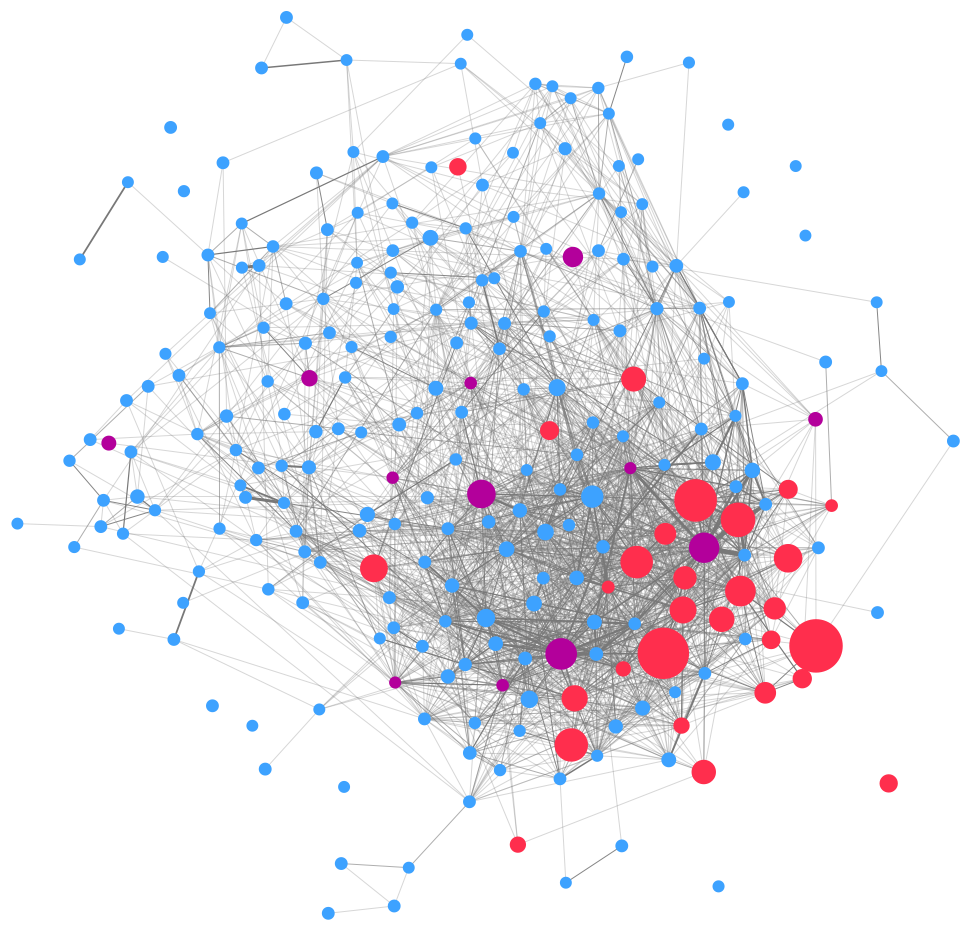
\includegraphics[scale=0.38]{imgs/Institutions.png}
\end{center}
\caption[Firm projection of the directorate network in New York City, 1902]{Firm projection of the directorate network in New York City, 1902. Blue nodes represent financial institutions, red nodes represent railways, and purple nodes represent insurance companies. The size of each node refers to its book value.}
\label{1902firms}
\end{figure}

The average membership in each aspect is calculated. For the financial industry the average membership is $17.21$, for the railroad industry the average membership is $12.76$, and the average membership for insurance companies is $26.17$. Therefore we note that railroads have, on average, lower number of directors and therefore a larger dependence on the directors that they have. Indeed, on average, a director of a railroad company will have a higher influence than a similar director of either a bank or an insurance company \emph{ceteris paribus}.

\paragraph{Aspectual distance.}

The distance of a pair of aspects measures their relatedness in terms of the number of connections that are similar in both aspects as a proportion of all connections in both aspects. During this time in America there existed no institutions regulating the formation of the directorate network. Given this free-market nature, one would expect that intertwining between aspects of the directorate network be reflective of complementarities between industries. Indeed, directors can attain a relatively large payoff from directly operating in industries that are have complementarities.

The distance between each pair of aspects was calculated. The distance from the banking industry to the railroad industry is given as $0.0127$ and $0.0249$ vice versa. The distance from the banking industry to the insurance industry is given as $0.0298$ and $0.0437$ vice versa. Finally, the distance from the railroad industry to the insurance industry is given as $0.0201$ and $0.0221$ vice versa.

\subsection{Centrality of directors and firms}

Microscopic network analysis focuses on the centrality of nodes. Of particular interest is the $\beta$-measure and standard degree measures, as discussed above. We provide an overview of the centrality of individual firms and directors.

\paragraph{$\beta$-measure of directors.}

With the original beta measure a number of directors are indicated as important, these include James Stillman ($1.436$), Edward H. Harriman ($0.988$) George F. Baker ($0.969$), Charles W. Morse ($0.8759$), and William Rockefeller ($0.861$).

It is undeniable that the men highlighted by the $\beta$-measure were highly influential during this time. On James Stillman's death in 1918 he was regarded as one of the wealthiest men in America, with an estimated fortune of \$100,000,000. Although closely tied to the activities of other influential financiers and industrialists such as J.P. Morgan, Edward H. Harriman, and William Rockefeller, his activities were never the subject of public discussion (New York Times, 1918). Between 1902 and the time of Edward H. Harriman's death in 1909 he remained President of the Union Pacific and the Southern Pacific railroad companies, and further controlled the Saint Joseph and Grand Island railway, the Illinois Central railroad, the Central of Georgia railroad, the Pacific Steamship Company, and the Wells Fargo Express Company. Indeed, all directors that have high beta are known to have some financial, speculative, and industrial influence in the early 20th Century. Also, during the beginning of the 20th Century Charles W. Morse organised the so-called \emph{Ice Trust} and made a move to banking, later being affiliated with F. Augustus Heinze during the Panic of 1907. William Rockefeller, brother of J.D. Rockefeller, was a prominent figure in finance, railways, and oil.

\paragraph{$\beta$-measure of firms.}

When aggregating the beta scores of all directors of each firm a number emerge as prominent. Specifically the American Surety Company ($4.21$), the Equitable Life Insurance Society ($3.157$), the Hanover National Bank ($3.111$) the Knickerbocker Trust Company ($2.868$), and the United States Trust Company ($2.623$). The measure of an affiliations beta in this circumstance provides an indication of the number of firms it influences beyond itself. All firms with a high beta are known to be large, however using this method there is little sign of J.P. Morgan and Company.

Importantly there is also little sign of railroad companies when using the original beta measure. Indeed, despite their size and value, railroad companies tended to have fewer directors on average compared to insurance companies and trusts. The original beta measure has an inherent bias toward firms with a large number of directors who themselves are members of other directorates that have a low number of directors. This bias is partially handled with the augmented measure of influence provided in Section~\ref{Theory:Influence}, which takes into consideration the value of firms. Furthermore, the original beta does not consider a multidimensional network.

% Standard degree measure...??

\subsection{Influence and elites in New York City}

Sections~\ref{Theory:Influence} and~\ref{Theory:Elites} introduced a number of tools to assess power and influence in a bipartite network, including the $\sigma$-score and elites. These are applied to the directorate network and the results are assessed below.

\subsubsection*{Firm value and influence}

With respect to the $\beta$-measure, we assumed that the value of all firms is equal to $1$. This assumption is dropped as we now note that the value of some firm $H \in \Gamma$ is equal to $\nu_{H}$. The use of a firms value with regards the $\sigma$-score diminishes the problem of the $\beta$-measure of over-biasing directors who are present on the boards of many small firms, or alternatively under-biasing firms that have a low number of directors but are also on the board of large and high valued firms.

\paragraph{Firm data.}

There are a number of ways to measure the \emph{value} of a firm. Here, we suggest that a firms' value is measured in terms of the book value of its resources. Data was collected from multiple sources. Specifically, data on the asset value of New York City trusts companies, safe deposit companies, and savings banks were gathered from the \emph{Reports of the Superintendent of Banks}, data on National Banks operating in New York were gathered from the \emph{Annual Reports of the Comptroller of the Currency to the Congress of the United States}, which were also published for each year of the analysis. Furthermore, data on the condition of commercial banks operating in New York was compiled by the New York Clearing House and published by the \emph{New York Times}\footnote{The New York Times have published their entire archive of newspapers since 1851 online.} alongside the publication of the Reports of the Superintendent of Banks. Data on the book value of insurance companies was gathered from the \emph{Annual Report of the Superintendent of Insurance to the New York Legislature}. More information regarding the sources can be seen in Table~\ref{vardesc}.

Each of these reports records the balance sheets of individual financial institutions. Specifically, the figures for the book value of resources and liabilities are provided and compartmentalised into separate types of assets and liabilities depending on the type of resources and liabilities in each banks balance sheet. Due to the fact that total resources and total liabilities are recorded for all financial institutions these values are used as the value of each firm.

Alternatively the Market Capitalisation of each firm could be used derived from the share value and number of shares outstanding in each company; however there are three main issues with using this data: (1) The majority of all recorded financial institutions were not publicly floated on the stock market, and therefore the share price and market capitalisation of these institutions are unknown; (2) Out of the financial institutions that were floated the information regarding the number of shares outstanding is still only partial; and (3) The reports published regarding the financial institutions adjusted the book value of their assets and liabilities such that they would better reflect their market values.

\paragraph{Influence of directors.}

The (weighted) $\sigma$-score measures the influence of directors in terms of dollar amounts\footnote{Note that these are non-normalised weighted $\sigma$-scores.}. Specifically, the influence of a director will be proportional to the value of all firms that they are a member of and the number of directors of each firm. When running the measurement, the directors with the highest influence include James Stillman ($222,163,741.5$), Edward H. Harriman ($221,102,348.2$), Hamilton Twombly ($167,033,722.2$), James J. Hill ($161,756,194.5$), and Samuel Rea ($141,321,877.5$).

Although Stillman and Harriman were notable with the beta measure, the introduction of Twombly, Hill, and Rea suggests the removal of bias against directors of railroads which were valued highly, but had a relatively low number of directors. Indeed, Hill was the CEO of Great Northern Railway during this time. Twombly was financial advisor to William Vanderbilt, and made a career in the railroad industry.

\paragraph{Influence of firms.}

The influence of each firm will be given by the $\sigma$-score calculated from the directorate hypergraph. The top firms that emerge from this analysis are the Equitable Life Assurance Society ($1,698,309,975$), the Southern Pacific Company ($1,385,947,753$), the Union Pacific Railroad Company ($1,364,554,939$), the Northern Pacific Railway Company ($1,385,947,753$), and Baltimore and Ohio Railroad Company ($1,301,836,214$).

The Equitable Life Assurance Society remains consistently high in the ranking. However, many of the top firms are railroad companies, which suggests that, despite having a relatively low number of directors, the directors are also directors in other highly valued companies such as other railways and highly valued banks.

\subsubsection*{The elites of New York City}

Elites refer to nodes that exist in all aspects of an aspectual hypergraph. With respect to a directorate network, an elite refers to an agent that is a director of a set of firms such that all firms collectively operate in all industries. An elite network refers to the subsequent network that results from parsing out the elite. Further analysis can be done with respect to the resulting elite structure; indeed, some elites may be more important than others. This can be measured with respect to known centrality measures.

\begin{figure}[t]
\begin{center}
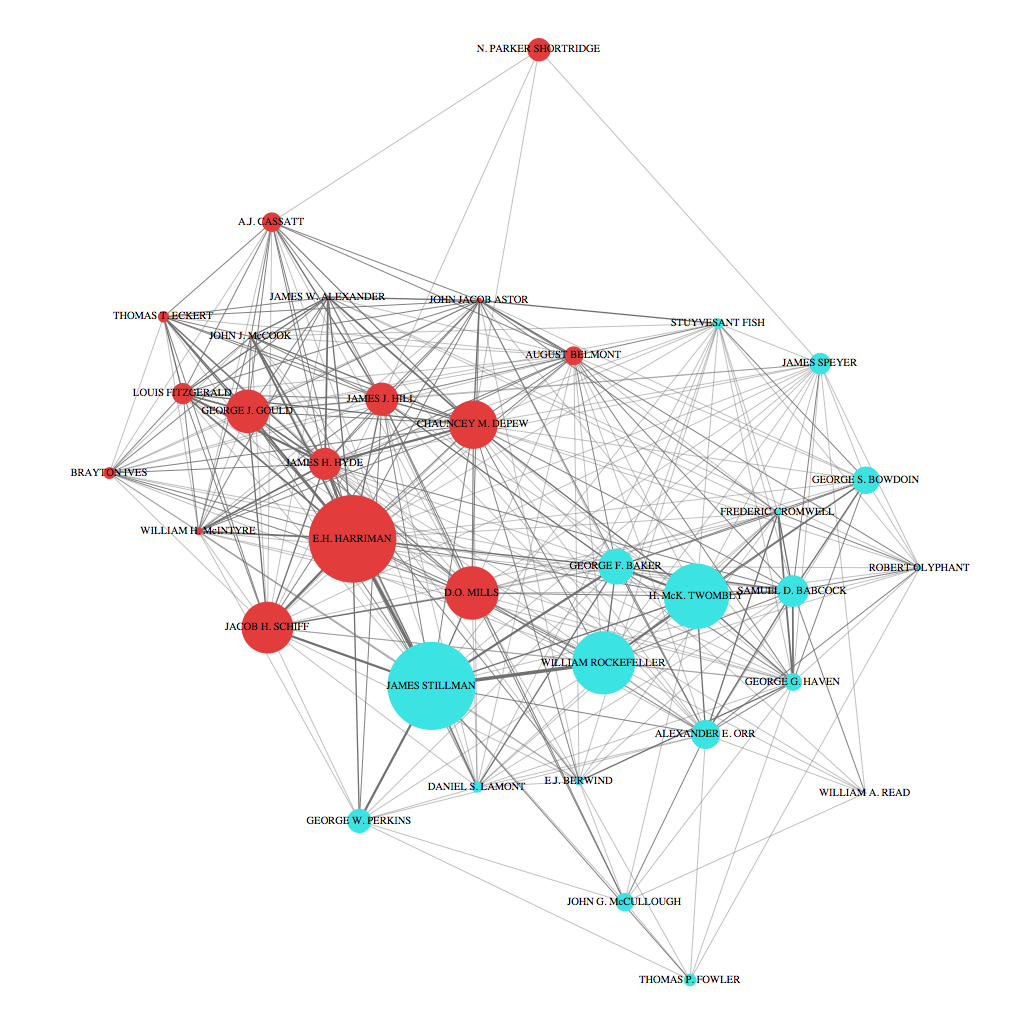
\includegraphics[scale=0.38]{imgs/Elite.png}
\end{center}
\caption[Elite directors in New York City, 1902]{Elite directors in New York City. The larger the node the greater the directors influence. The colour of the node represents the community it is a member of according to Newman's Q.}
\label{Fig:elite}
\end{figure}

The elite structure that emerges can be seen in Figure~\ref{Fig:elite}. There are a number of comments to be made. First, it is notable that from the initial network of $3006$ directors, only $35$ directors remain as elite. Second, the network much more dense with a density of $0.555$. There exists two tightly-knit cores resulting in two distinct communities when using Newman's Q-measure of modularity (Newman, 2006), which subsequently provides a value of $0.224$ for the entire network. These communities are highlighted in red and blue. Third, the diameter of the network is $3$, with an effective diameter of $2$, suggesting that any elite director can contact any other through a single intermediary\footnote{The notion of an effective diameter refers to the lowest resulting diameter after $10\%$ of the nodes in the network have been removed, and was initially proposed by Leskovec et al. (2005). When N. Parker Shortridge, William A. Read, and Thomas P. Fowler are removed from the elite network the diameter drops to 2.}. Finally, the average degree in the network is $18.857$, suggesting that on average each node is connected to over half the network, and the average weighted degree is $33.943$. The degree distribution is relatively normally distributed, with most directors having a degree between $16$ and $19$.

The emergence of elites and the resulting topology of the elite structure is notable due to its non-random nature. Indeed, although $99\%$ of the nodes and links have been removed from the director projection of the bipartite network the elite network that remains is both a single component and substantially more densely connected than the director projection of the bipartite network. This non-random nature indicates that there must exist some strategic network formation; specifically, there is utility to be gained from elites directly connecting to other elites. This could be in the form of both informational benefits and in the form of coordination benefits. Specifically, in this case, elites have direct access to information regarding the operations and the health of all industries and can therefore coordinate activities---such as investment, insurance, and funding---between and within industries.

As predicted, the elite directors have a high propensity to be influential. Specifically, eight out of the top ten most influential directors are elite and fourteen out of the top twenty-five are elite. Those directors who have a higher influence have a greater propensity to be more central in the elite structure when considering conventional centrality measures, whilst those directors with little influence are more peripheral.

The most central members of the elite also constitute a substantial number of the National Securities Company's members. Specifically, Stillman, Harriman, Schiff, Lamont, Baker, Hill, and Perkins were directors in the National Securities Company; and all play significantly central roles in the network. Even when removing the National Securities Company from the network and recalculating the elite, all directors remain notably central. This suggests, from purely case-study evidence, that elites were not only important for influence, but also control between industries.

\paragraph{Power and control in the elite.}

We look at measures of centrality for the elite network. There are a number of off-the-shelf measures to calculate the centrality of nodes within an undirected network. We also noted some measures, such as brokerage and criticality, which are specifically created to measure the power of individual nodes (brokerage) and sets of nodes (criticality).

We first look at off-the-shelf measures of centrality. Table~\ref{CentralElite} provides the centrality statistics for the 10 most central directors in the Elite structure. We note that although different centrality measures provide a slightly different ranking order than other centrality measures, there tends to be some consistency regarding the importance of Edward H. Harriman, James Stillman, Darius O. Mills, Chauncey M. Depew, and James J. Hill.

\begin{table}[t]
\resizebox{\textwidth}{!}{%
\centering
\begin{tabular}{ l c c c c c c} \hline
Director	           & $\delta_{i}$ 	& Weighted $\delta_{i}$ & Closeness   & Betweenness  & Eigenvector & Criticality \\ \hline
Edward H. Harriman	   &	$28$	&	$74$	       &	$0.850$	 &	$0.025$	    &	$0.997$	&	$0.401$\\
James H. Hyde	       &	$25$	&	$64$	       &	$0.790$	 &	$0.022$	    &	$0.898$	&	$0.364$\\
James Stillman	       &	$24$	&	$62$	       &	$0.772$	 &	$0.037$	&	$0.801$	&	$0.352$\\
Chauncey M. Depew	   &	$29$	&	$58$	       &	$0.871$	 &	$0.044$	&	$0.999$	&	$0.414$\\
George F. Baker	       &	$23$	&	$46$	       &	$0.755$	 &	$0.020$	&	$0.796$	&	$0.341$\\
James J. Hill	       &	$24$	&	$45$	       &	$0.772$	 &	$0.033$	&	$0.832$	&	$0.353$\\
Darius O. Mills	       &	$29$	&	$44$	       &	$0.871$	 &	$0.040$	&	$1.000$	&	$0.411$\\
John Jacob Astor	   &	$23$	&	$44$	       &	$0.755$	 &	$0.016$	&	$0.837$	&	$0.339$\\
Henry Twobley	       &	$19$	&	$43$	       &	$0.693$	 &	$0.009$	&	$0.677$	&	$0.288$\\
Jacob H. Schiff	       &	$24$	&	$41$	       &	$0.772$	 &	$0.016$	&	$0.870$	&	$0.340$\\ \hline
\end{tabular}
}
\caption{Centrality statistics of 10 most central directors in the elite structure.}
\label{CentralElite}
\end{table}

Due to the well-connected nature of the elite structure there are no middlemen and therefore no opportunity for brokerage. However, the incomplete nature of the network allows for the existence of blocks. When the criticality measure is applied the the elite structure we find that are the most important. Note that all but one of these individuals exist in the Northern Securities Company; indeed, it is acceptable to conclude that these directors could collectively control and manipulate main trusted channels of information between all industries of the economy.

\section{Economic performance and centrality} \label{Application:Regression}

Thus far we have developed tools to measure influence and elites and applied these to the directorate network of New York City. It was noted through the anecdotal evidence of the Northern Securities Company that elites have significant power in multiple industries of the economy, and that highly influential firms, i.e., firms with a large $\sigma$-score, were economically dominant. Here we assess whether these are general phenomena and thus answer the initial research question of whether the influence of a firms' directorate has an impact on its economic performance.

Of specific interest is the ability for a financial institution to generate profit and increase its size as a consequence of the centrality of a firms' directorate. As hypothesised above, the size and influence of the firms' directorate network should have an impact on the performance and profitability of the firm. This relationship may emerge from a number of sources, for example, from the ability for firms to borrow funds from other financial institutions to invest in entrepreneurial opportunities. Indeed, we would expect that a more connected financial institution would be able to exploit social relations, indicated by overlapping portfolios, and therefore reduce any uncertainty in the loan and investment opportunity. Although data from insurance, railroads, and banking are gathered the specific interest of this research is in financial institutions only.

\subsection{Overview of data}

The data gathered and analysed can be partitioned into two types: the first is the network data, and the second is balance-sheet data. The source of the network data has been discussed above; all centrality measures, apart from influence and external influence, were calculated from this data. This centrality data is complete for all firms and financial institutions. Balance-sheet data was acquired from multiple sources as discussed before. Data on the value of all financial institutions resources was attained, however data on the full balance sheet of each financial institution is incomplete.

\subsubsection*{Variable descriptions}

Descriptions of all variables used in the regression analysis are provided in Table~\ref{vardesc}. This table includes all relevant balance sheet data used in the analysis as well as dummy variables. There are two sets of dummy variables, the first set relates to the type of financial institution which includes State banks, National banks, Savings bank, and a Trust, and the second set relates to the location of the headquarters of the financial institution in either one of five boroughs of New York City, either Manhattan, Brooklyn, Queens, the Bronx, or Staten Island.

\begin{table}[t!]
\resizebox{\textwidth}{!}{%
\begin{tabular}{lll} \hline
{\bf Variable name}         & {\bf Description}                                                                                                                                                                    & {\bf Source} \\ \hline
Profits ($\pi_{i}$)               & Profits made by firm as indicated on January 1st 1903. & \emph{b,c,d}        \\
Size ($\nu_{i}$)                  & Size of the firm measured by the book value of the firms total assets.                                                                                                                                                             & \emph{b,c,d}        \\
\begin{tabular}[c]{@{}l@{}}Interbank\\ Borrowing\end{tabular}  & \begin{tabular}[c]{@{}l@{}}Total amount of money due to all other financial institutions in January\\ 1st 1903. This includes all money lent out to trust companies, savings banks,\\ State banks and National banks.\end{tabular} & \emph{b,c,d}        \\
Liquid                & \begin{tabular}[c]{@{}l@{}}Total amount of cash on hand. This includes all liquid assets such as specie,\\ banknotes, checks, and other cash items.\end{tabular}                                                                    & \emph{b,c,d}        \\
Illiquid              & Total amount of money held in the form of stocks, bonds, and mortgages.                                                                                                                                                             & \emph{b,c,d}        \\
\begin{tabular}[c]{@{}l@{}}Interbank\\ Lending\end{tabular} & \begin{tabular}[c]{@{}l@{}}Total amount of money lent out to all other banks including Savings banks,\\ State banks, National banks, and trust companies. Amounts recorded in \\ January 1st 1903.\end{tabular}                    & \emph{b,c,d}        \\
Year                  & The number of years that the firm has been operating.                                                                                                                                                                              & \emph{a}            \\
Directors             & Number of directors in the firm in September 1902.                                                                                                                                                                                 & \emph{a}            \\
$\sigma_{i}$              & The influence of a firm given by its $\sigma$-score.                                                                                                                                                                               & \emph{a,b,c,d,e}            \\
$\sigma^{\star}_{i}$                 & The external influence of a fir.                                                                                                                                                                                                  & \emph{a,b,c,d,e}            \\
Elites                & The number of elite directors in the firm.                                                                                                                                                                                         & \emph{a,e}            \\
$\beta^{\star}_{i}$   & The generalised $\beta$-measure of a firm in the affiliation projection.                                                                                                                                                                       & \emph{a,e}            \\
Criticality           & The criticality score of a firm in the affiliation projection.                                                                                                                                                                     & \emph{a,e}            \\
$\delta_{i}$          & \begin{tabular}[c]{@{}l@{}}The degree of the firm in the affiliation projection. The total number of \\ other firms that the firm has direct interlocks with.\end{tabular}                                                         & \emph{a, e}            \\
Weighted $\delta_{i}$ & The sum of all weighted interlocks with other firms in the affiliation network.                                                                                                                                                    & \emph{a,e}            \\
Cluster               & The local clustering coefficient of the firm in the affiliation projection.                                                                                                                                                        & \emph{a,e}            \\
PageRank              & The PageRank centrality of the firm in the affiliation projection.                                                                                                                                                                 & \emph{a,e}            \\
Closeness             & The normalised closeness centrality of the firm in the affiliation projection.                                                                                                                                                     & \emph{a,e}            \\
Betweenness           & The normalised betweenness centrality of the firm in the affiliation projection.                                                                                                                                                   & \emph{a,e}            \\
Eigenvector           & The weighted eigenvector centrality of the firm in the affiliation projection.                                                                                                                                                     & \emph{a,e}            \\
StateDum              & Dummy variable. Equal to $1$ if firm is a State Bank and $0$ otherwise.                                                                                                                                                                 & \emph{b,c,d}        \\
NatDum                & Dummy variable. Equal to $1$ if firm is a National Bank and $0$ otherwise.                                                                                                                                                            & \emph{b,c,d}        \\
SavingsDum            & Dummy variable. Equal to $1$ if firm is a Savings Bank and $0$ otherwise.                                                                                                                                                               & \emph{b,c,d}        \\
TrustDum              & Dummy variable. Equal to $1$ if firm is a Trust and $0$ otherwise.                                                                                                                                                                    & \emph{b,c,d}        \\
BronxDum              & Dummy variable. Equal to $1$ if firm is situated in the Bronx and $0$ otherwise.                                                                                                                                                      & \emph{a}            \\
BrookDum             & Dummy variable. Equal to $1$ if firm is situated in Brooklyn and $0$ otherwise.                                                                                                                                                       & \emph{a}            \\
ManhatDum             & Dummy variable. Equal to $1$ if firm is situated in Manhattan and $0$ otherwise.                                                                                                                                                      & \emph{a}            \\
QueensDum             & Dummy variable. Equal to $1$ if firm is situated in Queen's and $0$ otherwise.                                                                                                                                                        & \emph{a}            \\
StatenDum             & Dummy variable. Equal to $1$ if firm is situated in Staten Island and $0$ otherwise.                                                                                                                                                  & \emph{a}  \\ \hline
\end{tabular}
}
\begin{flushleft}
\emph{Note: `a' refers to the Directory of Directors of New York City, `b' refers to the Annual Report of the Superintendent of Banks 1903, `c' refers to the Annual Report of the Comptroller of the Currency 1902, `d' refers to the New York Times, and `e' refers to calculation.}
\end{flushleft}
\caption{Description of variables used for regression analysis}
\label{vardesc}
\end{table}

Data from bank balance sheets was analysed. Of specific interest was the total value of all liquid assets, such as specie, banknotes and other cash items, and illiquid assets, in the form of securities. So too were the financial institutions' interbank borrowing and lending characteristics.

A notable omission from the data is a measure of Tobin's Q, due to the inability to attain full stock market data of all institutions during this time. Other notable papers use Tobin's Q as an indicator to the health and economic performance of the firm. Indeed, future research regarding the relationship between directorate centrality and firm performance should take advantage of stock market data and derived measures such as Tobin's Q.

\subsubsection*{Data summary statistics}

The summary statistics of all variables used can be seen in Table~\ref{fin-ss} in Appendix~\ref{B}. The full network of financial institutions includes $63$ State banks, $49$ National banks, $51$ Savings banks, and $47$ trusts. Despite there being fewer trusts, they are more substantially connected than any other type of firm, including railroads and insurance companies. Indeed, firms are connected to $4.35$ different trusts on average, compared to $3.13$ National banks, $2.44$ State banks, and $1.7$ Savings banks.

On average financial institutions are connected to $15.51$ other firms through an overlapping directorate, however, much like other social and natural systems, the degree distribution is non-normal. Specifically, the frequency of nodes' degrees follows a distribution more akin to a power-law. Subsequently, most of the centrality measures, which are derived from the structure of the directorate hypergraph and affiliation projection, follow the same power-law distribution. All centrality measures have a skewed distribution suggesting that many firms have a low centrality, with a few having a relatively high centrality. Closeness centrality nor the $\beta$-measure follow the same power-law distributions as the other centrality measures. Closeness centrality is reflective of the density and average path length in the network, thus, with a well-connected network, many of the closeness centralities of individual firms are similar and converge to $1$ as the network densifies. The distribution of the $\beta$-measure has a negative kurtosis.

Data on the size and centrality of financial institutions is complete. However, balance sheet data was incomplete especially with respect to the interbank borrowing of savings banks.

\paragraph{Correlation matrix.}

The matrix in Table~\ref{fin-corr} shows dependence relationships of variables in the form of Pearson correlation coefficients between all pairs of financial data variables and important centrality measures used throughout the analysis.

A number of points are notable here. First, there exists only a weak positive correlation between the interbank borrowing and interbank lending of a financial firm, suggesting a a potential imbalance between the amount an institution borrows and the amount it lends, which implies the existence of surplus and deficit institutions. Second, there exists a high correlation between the size of a firm (the value of its total assets) and the interbank borrowing, the amount of liquid and illiquid assets of the firm. The inclusion of size and interbank borrowing, or any pairs of highly correlated variables, may bias the analysis. Third, all centrality measures are very highly correlated with each other. Again, the inclusion of all highly correlated centrality measures can bias the coefficients of the regression. Fourth, there exists high correlation between the size of the firm and all centrality measures. Finally, the relationship between the number of directors and profit is relatively low.

\begin{table}[t!]
\begin{onehalfspace}
\centering
\resizebox{\textwidth}{!}{%
\begin{tabular}{@{\extracolsep{5pt}} lcccccccccccccc}
\\[-1.8ex]\hline
\hline \\[-1.8ex]
                                                              & \begin{tabular}[c]{@{}c@{}}Profit\\($\pi_{i}$)\end{tabular} & \begin{tabular}[c]{@{}c@{}}Interbank\\borrowing\end{tabular} & Liquid & Illiquid & \begin{tabular}[c]{@{}c@{}}Interbank\\lending\end{tabular} & Years  & Directors & \begin{tabular}[c]{@{}c@{}}Size\\($\nu_{i}$)\end{tabular} & $\sigma_{i}$ & Elite & $\delta_{i}$ & \begin{tabular}[c]{@{}c@{}}Weighted\\ $\delta_{i}$\end{tabular} & Eigenvector & $\beta^{\star}_{i}$ \\ \hline
Profit ($\pi_{i}$)                                                        & 1.000  &                                                               &        &          &                                                             &        &           &       &              &       &              &                                                                 &             &             \\
\begin{tabular}[c]{@{}l@{}}Interbank\\ borrowing\end{tabular} & 0.181  & 1.000                                                         &        &          &                                                             &        &           &       &              &       &              &                                                                 &             &             \\
Liquid                                                        & 0.283  & 0.861                                                         & 1.000  &          &                                                             &        &           &       &              &       &              &                                                                 &             &             \\
Illiquid                                                      & 0.131  & 0.586                                                         & 0.113  & 1.000    &                                                             &        &           &       &              &       &              &                                                                 &             &             \\
\begin{tabular}[c]{@{}l@{}}Interbank\\ lending\end{tabular}   & 0.091  & 0.340                                                         & 0.200  & 0.342    & 1.000                                                       &        &           &       &              &       &              &                                                                 &             &             \\
Years                                                         & 0.142  & 0.321                                                         & 0.338  & 0.387    & 0.125                                                       & 1.000  &           &       &              &       &              &                                                                 &             &             \\
Directors                                                     & 0.045  & 0.028                                                         & -0.118 & 0.461    & 0.462                                                       & -0.091 & 1.000     &       &              &       &              &                                                                 &             &             \\
Size ($\nu_{i}$)                                                & 0.325  & 0.829                                                         & 0.708  & 0.600    & 0.384                                                       & 0.370  & 0.220     & 1.000 &              &       &              &                                                                 &             &             \\
$\sigma_{i}$                                                      & 0.185  & 0.391                                                         & 0.410  & 0.229    & 0.329                                                       & 0.087  & 0.298     & 0.612 & 1.000        &       &              &                                                                 &             &             \\
Elite                                                         & 0.108  & 0.260                                                         & 0.265  & 0.103    & 0.221                                                       & -0.014 & 0.276     & 0.441 & 0.902        & 1.000 &              &                                                                 &             &             \\
$\delta_{i}$                                                  & 0.168  & 0.320                                                         & 0.318  & 0.253    & 0.330                                                       & 0.048  & 0.352     & 0.535 & 0.860        & 0.789 & 1.000        &                                                                 &             &             \\
Weighted $\delta_{i}$                                         & 0.177  & 0.323                                                         & 0.327  & 0.237    & 0.314                                                       & 0.042  & 0.362     & 0.556 & 0.917        & 0.875 & 0.968        & 1.000                                                           &             &             \\
Eigenvector                                                   & 0.179  & 0.339                                                         & 0.354  & 0.231    & 0.298                                                       & 0.102  & 0.275     & 0.536 & 0.885        & 0.814 & 0.967        & 0.948                                                           & 1.000       &             \\
$\beta^{\star}_{i}$                                                   & 0.173  & 0.235                                                         & 0.188  & 0.211    & 0.260                                                       & -0.078 & 0.421     & 0.404 & 0.558        & 0.503 & 0.729        & 0.712                                                           & 0.592       & 1.000       \\
\hline \\[-1.8ex]
\end{tabular}
}
\caption{Correlation matrix of financial data and network centralities.}
\label{fin-corr}
\end{onehalfspace}
\end{table}


The assessment of the correlation matrix suggests that the $\sigma$-score, weighted degree, and eigenvector centralities should be most relevant in explaining the relationship between directorate centrality and economic performance. This is indeed highlighted with the regression analysis.

\subsection{Comparing financial institutions, insurance companies and railroads}

Before the regression analysis we provide a comparison of financial institutions, insurance companies, and railroads, noting fundamental differences between them. Figure~\ref{firm-type1} highlights differences in the variance between the size of the firms, the number of directors in the firm, and its influence. Notably, we find that the variance of the number of directors and value of banks is low relative to insurance companies and railroads. Insurance companies have a relatively high variance in the number of directors and railroads have a relatively high variance in the value of its assets.

\begin{figure}[t]
\label{firm-type1}
\centering
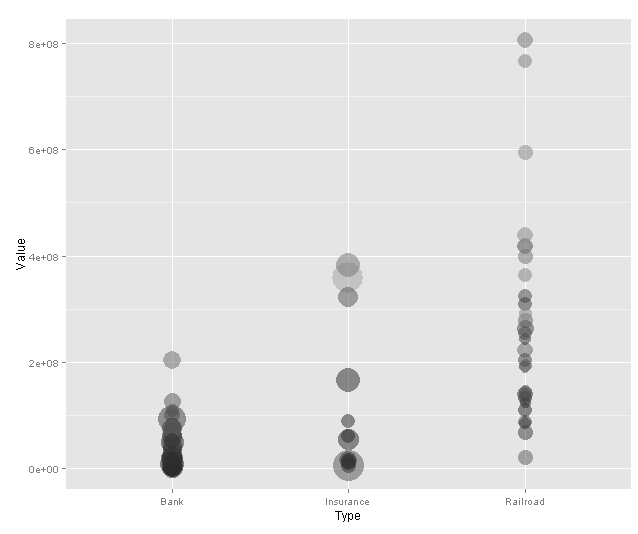
\includegraphics[width=0.7\textwidth]{imgs/firm-type2.png}
\caption{Distribution of firm value per industry}
\end{figure}

This assessment highlights that different types of firm can have substantially different fundamental characteristics. Notably, as is found below, the type of directorial overlap may matter more than the number of directorial overlaps.

\subsection{Regression analysis}

We use OLS regressions to assess the relationship between the centrality of the firm and the profits generated by it. A number of relationships are assessed; the first looks at the profits generated by the financial institutions and the centrality of the institutions' directorate, and the second investigates the size or value of the financial institutions assets and the centrality of the institution.

\subsubsection*{Profit and centrality}

The Regression model in Equation~\ref{eq:regprofit} is used to derive the relationship between a firms' directorate centrality and its profitability. Multiple centrality measures are used independent of each other and, as a consequence, we allow $Centrality_{i}$ to denote a form of centrality used in the specific regression. The centrality measures used in this analysis include the $\sigma$-score and number of Elites from the directorate hypergraph, the degree of the firm ($\delta$), eigenvector, $\beta$-measure and weighted degree from the affiliation projection. As a consequence, multiple regressions are used to find the relationship between profit and individual centrality measures. The regression equation is given by:

\begin{multline} \label{eq:regprofit}
\pi_{i} = b_{0} + b_{1}~Liquid_{i} + b_{2}~Illiquid_{i} + b_{3}~IBLending_{i} + b_{4}~Years^{2}_{i}\\
+ b_{5}~Directors_{i} + b_{6}~Centrality_{i} + \epsilon_{i}
\end{multline}
where $b_{v}$ is the co-efficient of the corresponding $v^{th}$ explanatory variable and $b_{0}$ is the intercept.

\paragraph{Interpretation of results.}

The result of the regressions can be seen in Table~\ref{regress:profit}. Each OLS regression includes 117 observations where all relevant data on financial institutions is complete. The total value of all liquid assets is quite consistent and highly statistically significant in all regressions regardless of centrality measure used. This suggests that as a firms' liquid assets increase by \$1,000,000 then the firms' profits should increase by approximately \$120,000. Moreover, the square of the number of years in operation is also consistent and statistically significant to 10\% and 5\% levels. This suggests that for every new year a firm is in operation its profit should increase by approximately \$10,000. All other variables, such as the total amount of Interbank lending, the total amount of Illiquid assets, and the number of directors all remain statistically insignificant at 10\% levels.

\begin{table}[t!] \centering
\resizebox{\textwidth}{!}{%
\begin{tabular}{@{\extracolsep{5pt}}lD{.}{.}{-3} D{.}{.}{-3} D{.}{.}{-3} D{.}{.}{-3} D{.}{.}{-3} D{.}{.}{-3} }
\\[-1.8ex]\hline
\hline \\[-1.8ex]
 & \multicolumn{6}{c}{\textit{Dependent variable:}} \\
\cline{2-7}
\\[-1.8ex] & \multicolumn{6}{c}{Profit ($\pi_{i}$)} \\
\\[-1.8ex] & \multicolumn{1}{c}{(1)} & \multicolumn{1}{c}{(2)} & \multicolumn{1}{c}{(3)} & \multicolumn{1}{c}{(4)} & \multicolumn{1}{c}{(5)} & \multicolumn{1}{c}{(6)}\\
\hline \\[-1.8ex]
 Liquid & 0.113^{***} & 0.117^{***} & 0.120^{***} & 0.118^{***} & 0.121^{***} & 0.123^{***} \\
  & (0.015) & (0.015) & (0.015) & (0.015) & (0.016) & (0.016) \\
  Illiquid & 0.002 & 0.004 & 0.008 & 0.005 & 0.008 & 0.010 \\
  & (0.013) & (0.013) & (0.013) & (0.013) & (0.013) & (0.013) \\
  IBLending & 0.043 & 0.042 & 0.040 & 0.044 & 0.037 & 0.037 \\
  & (0.034) & (0.034) & (0.035) & (0.035) & (0.035) & (0.036) \\
  Years$^2$ & 0.0001^{*} & 0.0001^{**} & 0.0001^{**} & 0.0001^{**} & 0.0001^{**} & 0.0001^{**} \\
  & (0.00003) & (0.00003) & (0.00003) & (0.00003) & (0.00003) & (0.00003) \\
  Directors & 0.004 & 0.005 & 0.007 & 0.003 & 0.009 & 0.009 \\
  & (0.013) & (0.013) & (0.013) & (0.013) & (0.013) & (0.015) \\
  $\sigma_{i}$ & 11.234^{***} &  &  &  &  &  \\
  & (3.727) &  &  &  &  &  \\
  $\sigma^{\star}_{i}$ &  & 10.589^{***} &  &  &  &  \\
  &  & (3.882) &  &  &  &  \\
  Elites &  &  & 0.070^{**} &  &  &  \\
  &  &  & (0.032) &  &  &  \\
  Weighted $\delta_{i}$ &  &  &  & 0.006^{**} &  &  \\
  &  &  &  & (0.002) &  &  \\
  $\delta_{i}$ &  &  &  &  & 0.006 &  \\
  &  &  &  &  & (0.004) &  \\
  $\beta^{\star}_{i}$ &  &  &  &  &  & 0.087 \\
  &  &  &  &  &  & (0.105) \\
  Constant & 0.071 & 0.062 & 0.044 & 0.030 & -0.021 & -0.019 \\
  & (0.188) & (0.190) & (0.191) & (0.189) & (0.191) & (0.193) \\
 \hline \\[-1.8ex]
Observations & \multicolumn{1}{c}{117} & \multicolumn{1}{c}{117} & \multicolumn{1}{c}{117} & \multicolumn{1}{c}{117} & \multicolumn{1}{c}{117} & \multicolumn{1}{c}{117} \\
R$^{2}$ & \multicolumn{1}{c}{0.625} & \multicolumn{1}{c}{0.620} & \multicolumn{1}{c}{0.612} & \multicolumn{1}{c}{0.615} & \multicolumn{1}{c}{0.602} & \multicolumn{1}{c}{0.597} \\
Adjusted R$^{2}$ & \multicolumn{1}{c}{0.605} & \multicolumn{1}{c}{0.599} & \multicolumn{1}{c}{0.591} & \multicolumn{1}{c}{0.594} & \multicolumn{1}{c}{0.580} & \multicolumn{1}{c}{0.575} \\
\hline
\hline \\[-1.8ex]
\textit{Note:}  & \multicolumn{6}{r}{$^{*}$p$<$0.1; $^{**}$p$<$0.05; $^{***}$p$<$0.01} \\
\end{tabular}
}
\caption{Results of profit-centrality regressions}
\label{regress:profit}
\end{table}

A number of centrality measures are tested, which include the $\sigma$-score of the financial institution, the number of elite directors in the institution, the degree and weighted degree of the institution, the institutions eigenvector and its $\beta$-measure. The $\sigma$-score has a positive, statistically significant relationship with the firms profit at a 99\% level, suggesting that as a firms influence increases by \$1,000,000 then its profit should increase by \$86,900. The number of elites has a positive, statistically significant relationship with the firms profit at a 95\% level, suggesting that as a firm increases the number of elites in its board by 1 it will lead to a generation of profits by \$70,000. Also, the weighted degree of a firm in the affiliation projection has a positive, statistically significant relationship with the firms profit at a 90\% level. This relationship suggests that if any one of a firms directors increases the number of boards that they are on by 1 then this will lead to an increase in profits by \$6,000.

Other recorded centrality measures, such as the degree of the firm, it's eigenvector centrality, and it's $\beta$-measure are all positively related to the firms profit, but none of which are statistically significant at a 90\% level. The insignificance of degree centrality suggests that the total number of overlapping directorates a firm has does not have an impact on its economic performance. Indeed, the number of links of the firm in the affiliation projection is not important to its profitability; rather the weight and the context of the links are more influential. Note that all other centrality measures, such as betweenness, closeness, PageRank, and the firms local clustering co-efficient were all tested but none of which are statistically significant to a 90\% level.

\paragraph{Location and firm-type dummies.}

The data consists of different types of financial institution, including National banks, State banks, Saving banks, and Trust companies. These financial institutions are located in different boroughs of New York City. Regressions are carried out to test the importance of firm type and location factors, the results of which can be seen in Table~\ref{profit-type-location} in Appendix~\ref{B}. The regression finds that National banks persistently have lower profit levels, suggesting that if a financial institution is a National bank then its profit will be approximately \$480,000 lower than other types of financial institution. All other firm-type and location dummies are recorded as statistically insignificant at the 90\% confidence level.

\paragraph{Interlock types.}

The initial regression showed that, in many cases, the centrality and connectivity of the financial institution was subsequently related to the institutions profits. We disaggregate the interlocks of each institution by counting the number of National banks, State banks, Savings banks, Trust companies, Insurance companies and Railroads each firm has an interlock with and perform a corresponding regression. The results can be seen in Table~\ref{profit-interlock-type} in Appendix~\ref{B}. We find that there is a positive, statistically significant relationship between the number of railroads a financial institution has an interlock with and the profitability of the financial institution. Specifically, we find that if a financial institution forms a new interlock with a railroad then this will generate an increase in profits of \$48,000. All other types of interlock are not found to be statistically significant at a 90\% level. This partitioning of a firms link set into firm types provides a deeper insight into the connectivity of the firm and may provide some explanation as to the inefficacy of the degree centrality to explain the profitability of the firm. Indeed, it may not be so simple as to suggest that the number of firms a financial institution is linked to is important; rather it can be seen that the type of firm a financial institution is connected to is also important. Such a concept is contained in the $\sigma$-score and $\sigma^{\star}$-score since, as noted above, railroads have a high value relative to other financial institutions and insurance companies.

Conversely, if a financial institution were to form an interlocking relation with a national bank then the profits of the firm will decrease by approximately \$60,000. All other types of interlock are not found to be statistically significant at a 90\% level. An explanation can be made for the negative relationship between National bank interlocks and low profit. We find that 13 out of 49 National banks have an above random number of interlocks with other National banks, these 13 firms with above random interlocks with other National banks are disproportionately low profit firms. Specifically, if we rank the set of National Banks in terms of profit we find that 9 out of the 13 National banks with larger than random interlocks are in the lower half of ranking order. Indeed, there exists positive assortative mixing of low profit National banks thus leading to the statistically significant finding.

To conclude, we note that the number of directorial overlaps does not have a statistically significant impact on the profitability of the financial institution. However, the type and context of the overlapping directorates matters for profitability, and this is not included in degree, eigenvector, beta, betweenness, or closeness centrality measures. We find that if firms are connected to more railroads then it will translate to a statistically significant increase in its profitability; firm type is captured in some way by nodal influence ($\sigma$) and external influence ($\sigma^{\star}$), therefore these centrality measure have statistically significant explanatory power.

\subsubsection*{Size and centrality}

Much like above we assess the relationship between the size of the financial institution in terms of the total value of its assets and its centrality, given by a number of different measures including the $\sigma$-score and number of elites. We follow much the same structure as the regression model in equation~\ref{eq:regprofit}, however we include interbank lending in this analysis. The resulting regression equation can be seen in Equation~\ref{eq:regsize} below:
\begin{multline} \label{eq:regsize}
\nu_{i} = \gamma_{0} + \gamma_{1}~Liquid_{i} + \gamma_{2}~Illiquid_{i} + \gamma_{3}~IBBorrowing_{i} + \gamma_{4}~IBLending_{i}\\
+ \gamma_{5}~Years^{2}_{i} + \gamma_{6}~Directors_{i} + \gamma_{7}~Centrality_{i} + \mu_{i}
\end{multline}
where $\gamma_{v}$ is the co-efficient of the corresponding $v^{th}$ explanatory variable and $\gamma_{0}$ is the intercept.

\paragraph{Interpretation of results.}

From the correlation matrix in Table~\ref{fin-corr} we found that the size of a firm was highly correlated with all centrality measures recorded, most specifically with the $\sigma$-score. This high correlation is to be expected since a firms $\sigma$-score is specifically dependent on its own size. The external influence of a firm, given by the $\sigma^{\star}$-measure is not dependent on the firms' own size, but the size of the firms that it has an overlapping directorate with.

The regression results can be seen in Table~\ref{reg:size}. With consideration to the non-centrality measures we find that the total amount of liquid assets, the total amount of illiquid assets, and the total amount of the financial institutions interbank borrowing is positively and significantly related to its value. This suggests that a firm that borrows more will have a higher value, which implies that firms of a larger size has an ability to borrow more. These results are robust across all centrality measures considered. Conversely, Interbank lending is inversely related to firm size, which is consistently significant to a 90\% confidence level in 4 out of 6 regression.

With regards to the centrality measures we find, unsurprisingly, that all measures are positively and significantly related to the size of the firm at 99\% levels and all generate an R$^2$ of over 0.8. When comparing centrality measures we find that the $\sigma$-score has the most explanatory power relative to the others. The weighted degree of a firm also has strong explanatory power, suggesting that if any one of a firms directors were to increase the number of directorates they participated in by 1 then this would lead to an increase of a firms size by \$279,000. Likewise, if a firm increased the number of elites in its directorate by 1 then this would be reflected in an increase in the size of the firm by \$2,977,000. Further, if a firms beta were to increase by 1 then this would lead to an increase in the size of the firm by \$7,160,000.

Other centrality measures---such as betweenness, eigenvector, and PageRank---are also statistically significant at a 99\% level. However, the local clustering co-efficient and closeness remain insignificant at a 90\% level.

\begin{table}[t] \centering
\resizebox{\textwidth}{!}{%
\begin{tabular}{@{\extracolsep{5pt}}lD{.}{.}{-3} D{.}{.}{-3} D{.}{.}{-3} D{.}{.}{-3} D{.}{.}{-3} D{.}{.}{-3} }
\\[-1.8ex]\hline
\hline \\[-1.8ex]
 & \multicolumn{6}{c}{\textit{Dependent variable:}} \\
\cline{2-7}
\\[-1.8ex] & \multicolumn{6}{c}{Size ($\nu_{i}$)} \\
\\[-1.8ex] & \multicolumn{1}{c}{(1)} & \multicolumn{1}{c}{(2)} & \multicolumn{1}{c}{(3)} & \multicolumn{1}{c}{(4)} & \multicolumn{1}{c}{(5)} & \multicolumn{1}{c}{(6)}\\
\hline \\[-1.8ex]
 Liquid & 1.410^{***} & 1.497^{***} & 1.760^{***} & 1.591^{***} & 1.669^{***} & 1.853^{***} \\
  & (0.477) & (0.492) & (0.505) & (0.484) & (0.505) & (0.524) \\
  Illiquid & 0.871^{***} & 0.946^{***} & 1.109^{***} & 0.932^{***} & 0.968^{***} & 1.113^{***} \\
  & (0.245) & (0.252) & (0.255) & (0.248) & (0.261) & (0.267) \\
  IBLending & -1.285^{*} & -1.381^{**} & -1.291^{*} & -1.078 & -1.270^{*} & -1.084 \\
  & (0.668) & (0.690) & (0.717) & (0.688) & (0.716) & (0.765) \\
  IBBorrowing & 1.307^{***} & 1.350^{***} & 1.236^{***} & 1.271^{***} & 1.279^{***} & 1.208^{***} \\
  & (0.237) & (0.245) & (0.253) & (0.242) & (0.252) & (0.264) \\
  Years$^2$ & 0.001 & 0.001 & 0.001^{*} & 0.001 & 0.001 & 0.001^{*} \\
  & (0.0005) & (0.001) & (0.001) & (0.001) & (0.001) & (0.001) \\
  Directors & 0.323 & 0.382 & 0.450^{*} & 0.223 & 0.362 & 0.293 \\
  & (0.238) & (0.245) & (0.253) & (0.251) & (0.258) & (0.290) \\
  $\sigma_{i}$ & 449.234^{***} &  &  &  &  &  \\
  & (69.721) &  &  &  &  &  \\
  $\sigma^{\star}_{i}$ &  & 417.640^{***} &  &  &  &  \\
  &  & (74.488) &  &  &  &  \\
  Elites &  &  & 2.977^{***} &  &  &  \\
  &  &  & (0.633) &  &  &  \\
  Weighted $\delta_{i}$ &  &  &  & 0.279^{***} &  &  \\
  &  &  &  & (0.047) &  &  \\
  $\delta_{i}$ &  &  &  &  & 0.390^{***} &  \\
  &  &  &  &  & (0.082) &  \\
  $\beta^{\star}_{i}$ &  &  &  &  &  & 7.160^{***} \\
  &  &  &  &  &  & (2.050) \\
  Constant & -1.584 & -2.021 & -2.485 & -3.011 & -5.100 & -4.952 \\
  & (3.594) & (3.713) & (3.836) & (3.641) & (3.779) & (3.932) \\
 \hline \\[-1.8ex]
Observations & \multicolumn{1}{c}{124} & \multicolumn{1}{c}{124} & \multicolumn{1}{c}{124} & \multicolumn{1}{c}{124} & \multicolumn{1}{c}{124} & \multicolumn{1}{c}{124} \\
R$^{2}$ & \multicolumn{1}{c}{0.856} & \multicolumn{1}{c}{0.846} & \multicolumn{1}{c}{0.835} & \multicolumn{1}{c}{0.850} & \multicolumn{1}{c}{0.836} & \multicolumn{1}{c}{0.823} \\
Adjusted R$^{2}$ & \multicolumn{1}{c}{0.847} & \multicolumn{1}{c}{0.836} & \multicolumn{1}{c}{0.825} & \multicolumn{1}{c}{0.840} & \multicolumn{1}{c}{0.826} & \multicolumn{1}{c}{0.812} \\
\hline
\hline \\[-1.8ex]
\textit{Note:}  & \multicolumn{6}{r}{$^{*}$p$<$0.1; $^{**}$p$<$0.05; $^{***}$p$<$0.01} \\
\end{tabular}
}
\caption{Results of size-centrality regressions}
\label{reg:size}
\end{table}

\paragraph{Location and firm-type dummies.}

Location and firm-type dummies are added to the regression analysis. As with the regression analysis of profit and centrality above we find that national banks have a persistently low size relative to state banks and trust companies. This persistent negative relationship to a firms size is statistically significant to a 95\% level. Specifically, we find that, when all other factors remain constant, if a financial institution is a national bank then the total value of its asset base will be approximately \$500,000 lower than if it were another type of financial institution. The location dummies are persistently insignificant and the centrality measures remain either statistically significant or insignificant as in Table~\ref{reg:size}.

\paragraph{Interlock types.}

We regress the aforementioned balance-sheet variables with firm types as with the analysis for profit and centrality. We find that there are no statistically significant relationships between the size of the financial institution and the types of firms that it has an overlapping directorate with. Indeed, the number of overlaps the firm participates in is of some significance as to the size of the firm, but unlike with profitability, the context of those linkages is insignificant.

\subsubsection*{Failure and centrality}

Data on the failure of National banks was gathered from the Annual Reports of the Comptroller of the Currency from 1902--1907. Altogether 16 out of 49 National banks failed during this period.

A probit model is used to test the causality between the characteristics of the National bank and whether it fails over this period.

\paragraph{Results.} We find that there exists no statistically significant relationship between the centrality of a firms directorate and the probability of firm failure over the subsequent 5 year period. We test individually each year up to 5 years and still find no result. Indeed, the centrality of the firm remains extremely insignificant.

\section{Concluding comments}

In this chapter we were interested in whether the influence and centrality of a firm had a significant impact on its economic performance, which was defined in terms of its profitability, size, and probability of failing within the next 5 years. Interest was focused on interlocking directorates during this time due to the institutional changes that emerged in 1914 which discouraged the formation of overlapping directorates. Congress claimed that certain institutions were engaged in too many, potentially uncompetitive, interlocks.

We first analysed centrality measures in hypergraphs and defined a bespoke measure of individual node and affiliation influence for weighted hypergraphs. The $\sigma$-score that was subsequently developed was seen as a generalisation of both the $\beta$-measure and the standard degree measure. We defined aspectual hypergraphs and noted the existence of elites and elite structures as potentially critical conduits of information.

Through a statistical analysis of the directorial hypergraph and an econometric analysis of firm performance, we note that the number of interlocks a financial institution is engaged with has no statistical significance on its economic performance. Rather, the context of these interlocks matters, which is captured by the $\sigma$-score and, to a degree, by the $\beta$-measure. Specifically, we find that financial institutions that have interlocks with high-value railways have significantly higher profits.

\paragraph{Future research.}

A number of novel research questions emerge from this analysis. We observed that the elite structure that emerged was non-random. The observation suggests that there must exist costs and payoffs such that a densely connected elite network forms in equilibrium. Appendix~\ref{AppD} proposes a model of \emph{elite network formation}, however much work and application is still required to justify the proposed network formation model. The model can be extended and applied to empirical cases of elite network formation over time.

\begin{subappendices}

\section[Degree and probabilistic eliteness]{Node degree and the probability of being elite} \label{AppA}

The number of elites in a network is important when considering elite structures and the distance between aspects. Here, we assess the weakly positive monotonic relationship between the degree of a node and the probability that it is elite. This can also be translated in terms of influence: intuitively, as a nodes influence increases its probability of becoming an elite must also increases in a non-linear fashion.

The probability that a node is an elite loosely follows a binomial distribution. Specifically, let the probability that some node $i \in N$ is an elite be denoted very literally as $Pr(i \in \mathcal{E})$ then, given that $| \Gamma_{i} | = h_{i}(\Gamma) > 0$ and $i$ has a number of connections possible, the probability is given by:
\[
Pr(i \in \mathcal{E}) = \frac{\mbox{Number of correct combinations of $b_{i}(\Gamma)$ links}}{\mbox{Total number of combinations of $b_{i}(\Gamma)$ links}}.
\]
The total number of connection combinations on affiliation set $\Gamma$ is given by $\binom{h}{h_{i}(\Gamma)}$. The number of `correct' combinations refers to the number of ways in which node $i$ can become an elite. As discussed above, there is a conditions on $i$ to become an elite and there is a restriction placed on the network.

\begin{abet}
\item The condition is that $\mathcal{A}_{i} = \mathcal{A}$, therefore $h^{A}_{i}(\Gamma) \geqslant 1 \, \forall \, A \in \mathcal{A}$.

\item The restriction is that $h^{A}_{i}(\Gamma) \leqslant \alpha_{A} \, \forall \, \ell \in K$.
\end{abet}
Due to (a) and (b) the probability of a node becoming elite deviates from the typical binomial distribution. The probability follows a multivariate hyper-geometric distribution with the following probability mass function (PMF):
\begin{equation} \label{eq:PMF}
Pr(i \in \mathcal{E}) =  \left[ \prod_{A = 1}^{a} \dbinom{\alpha_{A}}{h^{A}_{i}(\Gamma)} \right] \cdot \dbinom{h}{h_{i}(\Gamma)}^{-1},
\end{equation}
where $| \mathcal{A} | = a$. With the PMF in Equation~\ref{eq:PMF} we make the assumption that $h_{i}(\Gamma) \geqslant a$ and $\alpha_{A} \, \forall \, A \in \mathcal{A}$. Note that if $h_{i}(\Gamma) < a$ then $Pr(i \in \mathcal{E}) = 0$ due to the failure to satisfy condition (a).

All potential combinations for all $\alpha_{A}$ need to be assessed and plugged into the PMF above. For lack of a general formula to calculate the probability that a node is an elite given (a) and (b) an algorithm is developed to solve for the total number of correct combinations given $h_{i}(\Gamma) > 0$.

%\footnote{A MATLAB code is provided in Appendix which calculates the probability of a node becoming an elite. Variables in the code include the number of dimensions ($k$) and the number of affiliations ($m$).}

Before continuing with the algorithm we first define the set $C(h_{i}(\Gamma))$ as a set of affiliation combinations such that the number of affiliation is equal to $h_{i}(\Gamma)$. Formally,
\[
C(h_{i}(\Gamma)) = \left\{ \mathcal{H} \subseteq \Gamma \, \mid \, | \mathcal{H} | = h_{i}(\Gamma) \right\} .
\]
Note that there may be multiple distinct sets of affiliations that contain $h_{i}(\Gamma)$ distinct affiliations. We let the $v^{th}$ distinct set be denoted as $C^{v}(h_{i}(\Gamma))$. The algorithm is as follows:

\begin{abet}
\item[(1)] Construct the class $\mathcal{C}(h_{i}(\Gamma))$ as a set of sets containing all distinct sets of affiliations of size $h_{i}(\Gamma)$. Therefore:
\begin{align*}
\mathcal{C}(h_{i}(\Gamma)) & = \left\{ C(h_{i}(\Gamma)) \subseteq \Gamma \, \mid \, | C(h_{i}(\Gamma)) | = h_{i}(\Gamma) \right\}\\
                   & = \left\{C^{1}(h_{i}(\Gamma)), \ldots, C^{v}(h_{i}(\Gamma))\right\}
\end{align*}
in such a case $p = | \mathcal{C}(h_{i}(\Gamma)) | = \binom{m}{d_{i}}$.

\item[(2)] Construct sets $B \in \mathcal{C}(d_{i})$ such that all affiliations contained in each set $B$ are collectively members of all aspects. Therefore:
\[
B(h_{i}(\Gamma)) = \left\{ H \in \Gamma \, \mid \, B \cap A_{\ell} \neq \varnothing \, \forall \ell \in \mathcal{A} \mbox{ and } | B (h_{i}(\Gamma)) | = h_{i}(\Gamma) \right\} .
\]
Again, note that there may exist more than one set $B(h_{i}(\Gamma))$ that contains $h_{i}(\Gamma)$ distinct affiliations throughout all aspects. Similar to above, we let the $u^{th}$ distinct set be denoted as $H^{u}(h_{i}(\Gamma))$.

\item[(3)] Construct the class $\mathcal{H}(h_{i}(\Gamma)) \subseteq \mathcal{C}(h_{i}(\Gamma))$ as a set containing all $B(h_{i}(\Gamma))$. Therefore:
\[
\mathcal{B}(h_{i}(\Gamma)) = \left\{ B^{1}(h_{i}(\Gamma)), \ldots, B^{u}(h_{i}(\Gamma)) \right\}
\]
The set $\mathcal{B}(h_{i}(\Gamma))$ contains all combinations of affiliations that lead to node $i$ becoming an elite. If $h_{i}(\Gamma) < a$ then $\mathcal{B}(h_{i}(\Gamma)) = \varnothing$ and $u = 0$.

\item[(4)] Calculate:
\[
Pr(i \in \mathcal{E}) = \frac{ | \mathcal{B}(h_{i}(\Gamma)) |}{ | \mathcal{B}(h_{i}(\Gamma)) |} = \frac{u}{p} .
\]
\end{abet}

\begin{example} \label{ex:probelite}
Consider a hypergraph, $\Gamma$, with a set of nodes, $N$ where $|N| = 1$, a set of affiliations, $\Gamma$ where $| \Gamma | = 24$, and a set of aspects, $\mathcal{A}$ where $|\mathcal{A}| = 6$. The set of aspects are distributed evenly across all affiliations such that $\alpha_{A} = 4 \, \forall \, A \in \mathcal{A}$.
\end{example}

Note from Example~\ref{ex:probelite} above that the probability of node $i$ becoming an elite in weakly monotonic and loosely follows a typical binomial distribution.

\begin{proposition} \label{bounds}
Let $\Gamma$ be a hypergraph on node set $N$ and affiliation set $\Gamma$ where $i \in N$ and $|\Gamma| = h$. The set of aspects, $\mathcal{A}$ where $|\mathcal{A}| = a$, is distributed across all $H \in \Gamma$.

\begin{abet}
\item $Pr(i \in \mathcal{E}) = 1 \, \iff \, h_{i}(\Gamma) > h - \alpha_{\tilde{A}}$, where $\tilde{A}$ is the aspect $A \in \mathcal{A}$ that has the lowest number of affiliations distributed to it.

\item $Pr(i \in \mathcal{E}) = 0 \, \iff \, h_{i}(\Gamma) < h$.
\end{abet}
\end{proposition}

From Proposition~\ref{bounds} above we derive the upper and lower bounds. Specifically, we denote the upper bound by $\overline{b}$ where $h_{i}(\Gamma) = h$. Moreover, we denote the lower bound by $\underline{b}$, where $h_{i}(\Gamma) = h - \alpha_{\tilde{k}}$.

The upper bound for a non-normal distribution of aspects across affiliations will be higher than for a normal distribution. Since at the limit, as $h \rightarrow \infty$, the aspects are equally spread out across all affiliations; any skewness in the distribution will mean that some aspects will have less than $\frac{h}{a}$ affiliations allocated to them thus pushing the upper bound up. In empirical networks, such as those seen in Sections~\ref{Application:Network} and~\ref{Application:Regression}, aspects are rarely normally distributed.

\subsubsection*{Independent changes in aspects and affiliations}

Both increases in the number of affiliations and aspects suggests that the probability of any node becoming an elite given a degree between the upper and lower bounds will decrease. We see how changes in each variable independently impact the probability of becoming an elite. First, we consider a change in the number of aspects that exist in the network. If we are to assume there is a random distribution of aspects across all affiliations. If the number of aspects, $a$, increases across all affiliations then both the upper and lower bounds change. Specifically, an increase in the number of aspects pushes the lower bound to the right, increasing it by the change in $a$ exactly. An increase in the number of aspects increases the upper bound, assuming that the number of affiliations is maintained constant.

Second, we consider a change in the number of affiliations keeping all else constant. Note the condition that $m \geqslant k$. A change in the number of affiliations only changes the upper bound, suggesting that as the number of affiliations increases the upper bound increases by $\Delta h - \frac{a}{\Delta h}$, where $\Delta h = h' - h$. Differentiating the upper bound with respect to $h$ gives:
\[
\frac{\partial}{\partial h} \left( h - \frac{a}{h} \right) = \frac{a}{h^{2}} + 1 .
\]
Differentiating the upper bound with respect to $a$ gives
\[
\frac{\partial}{\partial a} \left( h - \frac{a}{h} \right) = - \frac{1}{h} .
\]
When the number of affiliations changes so too will the convergence from lower bound to upper bound. Specifically, as the difference between the upper and lower bounds diminishes the convergence will be faster and \emph{vice versa}. The slope therefore depends on the relationship $\frac{a}{h}$.

\subsubsection*{Changes in the distribution of aspects}

Empirical networks are not created randomly. Not only are the distribution of links for nodes and affiliations non-random, the distribution of aspects are typically non-random; some aspects may have more affiliations embedded than others.

For any given degree, number of affiliations, and number of aspects the probability of becoming an elite is highest when there is an even distribution of aspects across all affiliations. Therefore, for a given density the greatest number of elites occur when there is an even distribution of aspects. Where the distribution is skewed the of probability of becoming an elite falls since there will exist at least one aspect, $\tilde{a}$, such that $\alpha_{\tilde{a}} < \frac{h}{a}$. As this is so, the probability of having a link to an affiliation embedded within the aspect falls meaning that the overall probability of becoming an elite falls.

\subsubsection*{Simulations}

We provide some simulations on two different types of networks. In each type of network links are distributed in different ways, however in both types of network the aspects are distributed normally across all affiliations. The probability of being an elite is generated with respect to a random graph model with a fixed number of nodes and a fixed number of affiliations. The result of these simulations can be seen in Figure~\ref{RandSim1}.

\begin{figure}[h!]
\begin{center}
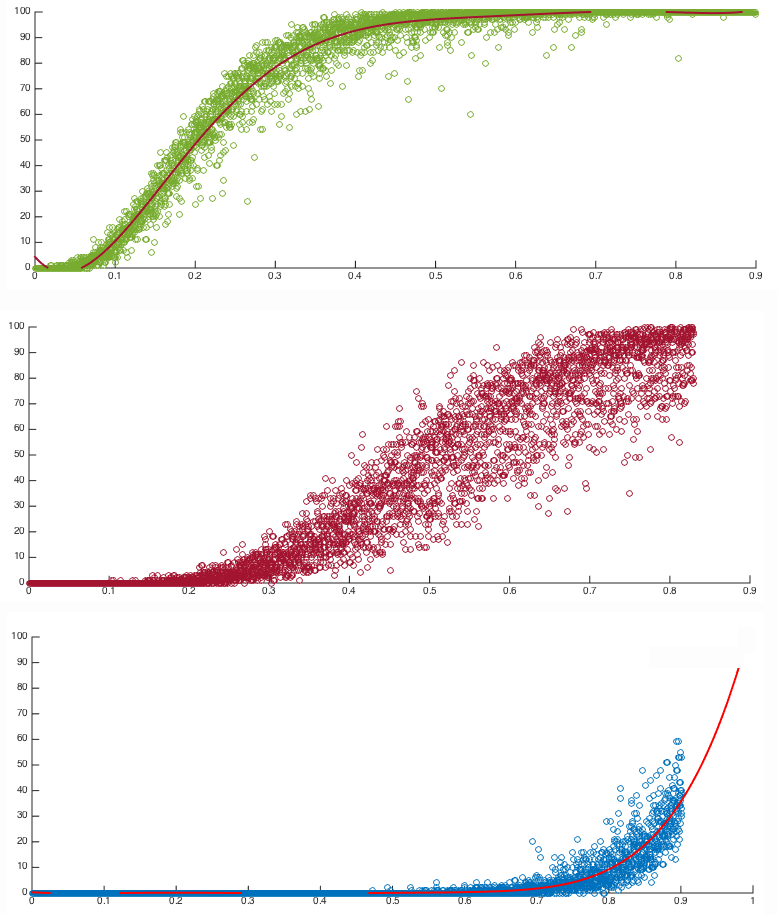
\includegraphics[scale=0.5]{imgs/RandSim1.png}
\end{center}
\caption[Probability distribution of a random node being an elite]{Simulation on a randomly generated network giving the probability of being an elite on the $y$-axis and the proportion of affiliations connected to on the $x$-axis. In all simulations the number of affiliations is 50. The top panel has 5 aspects; the middle panel has 10 aspects; and the bottom panel has 30 aspects.}
\label{RandSim1}
\end{figure}

\section[Additional information on data and regression analysis]{Additional information on data and regression analysis} \label{AppB}

Table~\ref{fin-ss} provides some summary statistics regarding all important variables used in the regression analysis throughout the econometric analysis in Section~\ref{Application:Regression}.

\begin{table}[h!]
\centering
\begin{tabular}{lccccc}
\\[-1.8ex]\hline
\hline \\[-1.8ex]
Statistic & \multicolumn{1}{c}{N} & \multicolumn{1}{c}{Mean} & \multicolumn{1}{c}{St. Dev.} & \multicolumn{1}{c}{Min} & \multicolumn{1}{c}{Max} \\
\hline \\[-1.8ex]
Profits ($\pi_{i}$) & 121 & 0.694 & 1.046 & 0.004 & 32 \\
Size ($\nu_{i}$) & 210 & 19.147 & 24.164 & 0.200 & 202.816 \\
Liquid & 174 & 1.536 & 3.811 & 0.000 & 27.753 \\
Illiquid & 174 & 6.813 & 13.722 & 0.001 & 85.937 \\
\begin{tabular}[c]{@{}l@{}}Interbank\\ borrowing\end{tabular} & 125 & 4.084 & 8.946 & 0.000 & 45.617 \\
\begin{tabular}[c]{@{}l@{}}Interbank\\ lending\end{tabular} & 174 & 1.202 & 1.789 & 0.000 & 12.568 \\
Years & 210 & 32.319 & 24.447 & 0 & 103 \\
Directors & 210 & 15.729 & 5.949 & 5 & 43 \\
$\sigma_{i}$ & 210 & 0.010 & 0.015 & 0.0001 & 0.088 \\
ExInf & 210 & 106,010,348 & 187,855,204 & 0.000 & 1,118,208,807 \\
Elites & 210 & 0.719 & 1.587 & 0 & 11 \\
$\delta_{i}$ & 210 & 15.514 & 15.206 & 0 & 71 \\
Weighted $\delta_{i}$ & 210 & 22.229 & 24.493 & 0 & 132 \\
Cluster & 210 & 0.336 & 0.246 & 0.000 & 1.000 \\
PageRank & 210 & 0.004 & 0.002 & 0.001 & 0.012 \\
Close & 210 & 0.371 & 0.101 & 0.000 & 0.522 \\
Between & 210 & 0.006 & 0.007 & 0.000 & 0.034 \\
Eigenvector & 210 & 0.173 & 0.226 & 0.000 & 0.965 \\
Beta & 210 & 0.925 & 0.647 & 0.000 & 3.111 \\
NatBanks & 210 & 3.129 & 3.383 & 0 & 16 \\
StateBank & 210 & 2.443 & 2.430 & 0 & 11 \\
SavingBank & 210 & 1.700 & 1.622 & 0 & 7 \\
Trusts & 210 & 4.348 & 4.578 & 0 & 21 \\
Railroad & 210 & 2.362 & 4.117 & 0 & 19 \\
Insurance & 210 & 1.533 & 1.998 & 0 & 8 \\
StateDum & 210 & 0.300 & 0.459 & 0 & 1 \\
NatDum & 210 & 0.233 & 0.424 & 0 & 1 \\
SavingsDum & 210 & 0.243 & 0.430 & 0 & 1 \\
TrustDum & 210 & 0.224 & 0.418 & 0 & 1 \\
BronxDum & 210 & 0.010 & 0.097 & 0 & 1 \\
BrooklynDum & 210 & 0.214 & 0.411 & 0 & 1 \\
ManhatDum & 210 & 0.690 & 0.463 & 0 & 1 \\
QueensDum & 210 & 0.038 & 0.192 & 0 & 1 \\
StatenDum & 210 & 0.019 & 0.137 & 0 & 1 \\
\hline \\[-1.8ex]
\end{tabular}
\label{fin-ss}
\caption{Summary statistics of important variables}
\end{table}

Table~\ref{profit-type-location} shows the regression results of profit and centrality where there are firm-type and location dummies.

\begin{table}[h!]
\centering
  \resizebox{\textwidth}{!}{%
\begin{tabular}{@{\extracolsep{5pt}}lD{.}{.}{-3} D{.}{.}{-3} D{.}{.}{-3} D{.}{.}{-3} D{.}{.}{-3} D{.}{.}{-3} }
\\[-1.8ex]\hline
\hline \\[-1.8ex]
 & \multicolumn{6}{c}{\textit{Dependent variable:}} \\
\cline{2-7}
\\[-1.8ex] & \multicolumn{6}{c}{Profit ($\pi_{i}$)} \\
\\[-1.8ex] & \multicolumn{1}{c}{(1)} & \multicolumn{1}{c}{(2)} & \multicolumn{1}{c}{(3)} & \multicolumn{1}{c}{(4)} & \multicolumn{1}{c}{(5)} & \multicolumn{1}{c}{(6)}\\
\hline \\[-1.8ex]
 Liquid & 0.129^{***} & 0.135^{***} & 0.134^{***} & 0.134^{***} & 0.133^{***} & 0.133^{***} \\
  & (0.017) & (0.018) & (0.018) & (0.018) & (0.018) & (0.018) \\
  Illiquid & -0.003 & 0.006 & 0.004 & 0.002 & 0.006 & 0.004 \\
  & (0.013) & (0.013) & (0.013) & (0.013) & (0.013) & (0.013) \\
  IBL & 0.068^{**} & 0.058 & 0.059 & 0.068^{*} & 0.054 & 0.063^{*} \\
  & (0.034) & (0.036) & (0.037) & (0.036) & (0.036) & (0.037) \\
  Years2 & 0.0001^{**} & 0.0001^{***} & 0.0001^{***} & 0.0001^{***} & 0.0001^{***} & 0.0001^{***} \\
  & (0.00003) & (0.00003) & (0.00003) & (0.00003) & (0.00003) & (0.00003) \\
  NumDir & -0.020 & -0.014 & -0.014 & -0.021 & -0.012 & -0.017 \\
  & (0.015) & (0.016) & (0.016) & (0.016) & (0.016) & (0.017) \\
  StateDum & -0.041 & -0.078 & -0.057 & -0.054 & -0.077 & -0.053 \\
  & (0.212) & (0.222) & (0.224) & (0.220) & (0.224) & (0.224) \\
  NatDum & -0.459^{**} & -0.483^{**} & -0.484^{**} & -0.491^{**} & -0.489^{**} & -0.490^{**} \\
  & (0.212) & (0.222) & (0.223) & (0.219) & (0.223) & (0.223) \\
  Railroad & -0.069^{**} & 0.003 & 0.013 & -0.014 & 0.032 & 0.019 \\
  & (0.031) & (0.024) & (0.023) & (0.023) & (0.030) & (0.014) \\
  BronxDum & -0.737 & -0.714 & -0.742 & -0.727 & -0.737 & -0.766 \\
  & (0.521) & (0.546) & (0.547) & (0.538) & (0.547) & (0.547) \\
  BrooklynDum & -0.311 & -0.287 & -0.301 & -0.321 & -0.280 & -0.313 \\
  & (0.346) & (0.362) & (0.364) & (0.358) & (0.364) & (0.364) \\
  ManhatDum & -0.433 & -0.481 & -0.540 & -0.510 & -0.511 & -0.535 \\
  & (0.337) & (0.355) & (0.355) & (0.348) & (0.355) & (0.353) \\
  QueensDum & -0.351 & -0.372 & -0.385 & -0.336 & -0.371 & -0.353 \\
  & (0.510) & (0.534) & (0.536) & (0.528) & (0.537) & (0.537) \\
  StatenDum & -0.199 & -0.237 & -0.244 & -0.170 & -0.268 & -0.232 \\
  & (0.637) & (0.668) & (0.671) & (0.661) & (0.670) & (0.670) \\
  $\sigma_{i}$ & 28.877^{***} &  &  &  &  &  \\
  & (8.791) &  &  &  &  &  \\
  Elite &  & 0.055 &  &  &  &  \\
  &  & (0.057) &  &  &  &  \\
  $\delta_{i}$ &  &  & 0.004 &  &  &  \\
  &  &  & (0.008) &  &  &  \\
  Weighted $\delta_{i}$ &  &  &  & 0.008^{*} &  &  \\
  &  &  &  & (0.004) &  &  \\
  Eigenvector &  &  &  &  & -0.212 &  \\
  &  &  &  &  & (0.598) &  \\
  $\beta_{i}$ &  &  &  &  &  & 0.078 \\
  &  &  &  &  &  & (0.113) \\
  Constant & 0.980^{**} & 0.953^{**} & 0.955^{**} & 0.967^{**} & 0.957^{**} & 0.963^{**} \\
  & (0.432) & (0.452) & (0.454) & (0.447) & (0.454) & (0.454) \\
 \hline \\[-1.8ex]
Observations & \multicolumn{1}{c}{117} & \multicolumn{1}{c}{117} & \multicolumn{1}{c}{117} & \multicolumn{1}{c}{117} & \multicolumn{1}{c}{117} & \multicolumn{1}{c}{117} \\
R$^{2}$ & \multicolumn{1}{c}{0.684} & \multicolumn{1}{c}{0.654} & \multicolumn{1}{c}{0.651} & \multicolumn{1}{c}{0.662} & \multicolumn{1}{c}{0.651} & \multicolumn{1}{c}{0.652} \\
Adjusted R$^{2}$ & \multicolumn{1}{c}{0.641} & \multicolumn{1}{c}{0.606} & \multicolumn{1}{c}{0.603} & \multicolumn{1}{c}{0.616} & \multicolumn{1}{c}{0.603} & \multicolumn{1}{c}{0.604} \\
\hline
\hline \\[-1.8ex]
\textit{Note:}  & \multicolumn{6}{r}{$^{*}$p$<$0.1; $^{**}$p$<$0.05; $^{***}$p$<$0.01} \\
\end{tabular}
}
\caption{Results of Profit-Centrality regressions with firm type and location dummies}
\label{profit-type-location}
\end{table}

Table~\ref{profit-interlock-type} shows the regression results of profit and centrality where the interlock types of each firm are categorised.

\begin{table}[h!]
\centering
  \resizebox{\textwidth}{!}{%
\begin{tabular}{@{\extracolsep{5pt}}lD{.}{.}{-3} D{.}{.}{-3} D{.}{.}{-3} D{.}{.}{-3} D{.}{.}{-3} D{.}{.}{-3} D{.}{.}{-3} }
\\[-1.8ex]\hline
\hline \\[-1.8ex]
 & \multicolumn{7}{c}{\textit{Dependent variable:}} \\
\cline{2-8}
\\[-1.8ex] & \multicolumn{7}{c}{Profit ($\pi_{i}$)} \\
\\[-1.8ex] & \multicolumn{1}{c}{(1)} & \multicolumn{1}{c}{(2)} & \multicolumn{1}{c}{(3)} & \multicolumn{1}{c}{(4)} & \multicolumn{1}{c}{(5)} & \multicolumn{1}{c}{(6)} & \multicolumn{1}{c}{(7)}\\
\hline \\[-1.8ex]
 Liquid & 0.106^{***} & 0.109^{***} & 0.104^{***} & 0.108^{***} & 0.104^{***} & 0.104^{***} & 0.104^{***} \\
  & (0.017) & (0.018) & (0.018) & (0.017) & (0.018) & (0.018) & (0.018) \\
  Illiquid & 0.004 & 0.014 & 0.014 & 0.011 & 0.013 & 0.015 & 0.014 \\
  & (0.013) & (0.014) & (0.014) & (0.013) & (0.014) & (0.014) & (0.014) \\
  IBL & 0.046 & 0.038 & 0.030 & 0.050 & 0.031 & 0.028 & 0.030 \\
  & (0.034) & (0.036) & (0.036) & (0.035) & (0.036) & (0.037) & (0.036) \\
  Years2 & 0.00004 & 0.0001^{**} & 0.0001^{**} & 0.0001^{**} & 0.0001^{**} & 0.0001^{*} & 0.0001^{**} \\
  & (0.00003) & (0.00003) & (0.00003) & (0.00003) & (0.00003) & (0.00003) & (0.00003) \\
  NumDir & -0.003 & 0.001 & 0.004 & -0.007 & 0.002 & 0.006 & 0.004 \\
  & (0.014) & (0.014) & (0.014) & (0.014) & (0.015) & (0.015) & (0.014) \\
  NatBanks & -0.042 & -0.054 & -0.037 & -0.069^{**} & -0.051 & -0.060 & -0.060^{*} \\
  & (0.035) & (0.036) & (0.071) & (0.034) & (0.042) & (0.036) & (0.036) \\
  StateBank & 0.021 & 0.042 & 0.070 & -0.006 & 0.046 & 0.053 & 0.047 \\
  & (0.033) & (0.033) & (0.064) & (0.036) & (0.033) & (0.038) & (0.033) \\
  SavingBank & 0.054 & 0.063 & 0.073 & 0.028 & 0.053 & 0.058 & 0.050 \\
  & (0.042) & (0.045) & (0.074) & (0.043) & (0.045) & (0.050) & (0.044) \\
  Trusts & -0.010 & -0.014 & 0.026 & -0.060^{**} & 0.014 & 0.003 & 0.003 \\
  & (0.022) & (0.025) & (0.071) & (0.029) & (0.032) & (0.022) & (0.022) \\
  Railroad & -0.047 & 0.019 & 0.071 & -0.021 & 0.065 & 0.048^{**} & 0.048^{**} \\
  & (0.036) & (0.030) & (0.067) & (0.030) & (0.044) & (0.022) & (0.022) \\
  Insurance & -0.024 & -0.014 &  & -0.048 & -0.010 & -0.022 & -0.023 \\
  & (0.054) & (0.056) &  & (0.054) & (0.064) & (0.057) & (0.056) \\
  Constant & 0.184 & 0.086 & 0.037 & 0.204 & 0.041 & 0.029 & 0.037 \\
  & (0.191) & (0.196) & (0.194) & (0.193) & (0.195) & (0.197) & (0.194) \\
  SigmaI & 30.457^{***} &  &  &  &  &  &  \\
  & (9.343) &  &  &  &  &  &  \\
  Elite &  & 0.096 &  &  &  &  &  \\
  &  & (0.065) &  &  &  &  &  \\
  D &  &  & -0.023 &  &  &  &  \\
  &  &  & (0.056) &  &  &  &  \\
  WD &  &  &  & 0.029^{***} &  &  &  \\
  &  &  &  & (0.009) &  &  &  \\
  Eigen &  &  &  &  & -0.716 &  &  \\
  &  &  &  &  & (1.559) &  &  \\
  Beta &  &  &  &  &  & -0.056 &  \\
  &  &  &  &  &  & (0.165) &  \\
 \hline \\[-1.8ex]
Observations & \multicolumn{1}{c}{117} & \multicolumn{1}{c}{117} & \multicolumn{1}{c}{117} & \multicolumn{1}{c}{117} & \multicolumn{1}{c}{117} & \multicolumn{1}{c}{117} & \multicolumn{1}{c}{117} \\
R$^{2}$ & \multicolumn{1}{c}{0.656} & \multicolumn{1}{c}{0.628} & \multicolumn{1}{c}{0.620} & \multicolumn{1}{c}{0.656} & \multicolumn{1}{c}{0.621} & \multicolumn{1}{c}{0.621} & \multicolumn{1}{c}{0.620} \\
Adjusted R$^{2}$ & \multicolumn{1}{c}{0.616} & \multicolumn{1}{c}{0.585} & \multicolumn{1}{c}{0.581} & \multicolumn{1}{c}{0.617} & \multicolumn{1}{c}{0.577} & \multicolumn{1}{c}{0.577} & \multicolumn{1}{c}{0.581} \\
\hline
\hline \\[-1.8ex]
\textit{Note:}  & \multicolumn{7}{r}{$^{*}$p$<$0.1; $^{**}$p$<$0.05; $^{***}$p$<$0.01} \\
\end{tabular}
}
\caption{Results of Profit-Centrality regressions with categorisation of interlocks}
\label{profit-interlock-type}
\end{table}


\section{Interlocking directorate formation} \label{AppD}

We provide a simple model of interlocking directorate formation on a weighted hypergraph. The weighted hypergraph consists of a set of nodes and a set of affiliations whereby each affiliation has a value attached. These concepts are defined above.

The primary goal of studying this model is to anticipate the structure of the directorate hypergraph and its network projections. Our specific interest is on the incentives of individual nodes in the formation of overlapping affiliations and the emergent structure from these incentives. From this we can give some insight regarding the connectivity of the directorate hypergraph and elite nodes, and can test the insights on the subsequent data analysis.

Within this formation situation individual nodes attempt to maximise their payoff and in doing so organise themselves into affiliations. In constructing the model we make a number of simplifying assumptions and argue their realism. First, we assume that each node is purely individualistic and, as a consequence, they do not consider the utilities of other agents; even those that operate in the same affiliation. Second, we argue that the utility of an individual node is derived directly from their influence in the hypergraph---which is well-defined by the $\sigma$-score---and indirectly from the influence of their neighbours. Third, we make the assumption that the inclusion of some node into an affiliation must benefit all incumbent members of the affiliation individually. Indeed, consent is required from all $i \in H$ so that $j \notin H$ can join $H$. Finally, we note that the indirect influence, or benefit, that some node $i \in N$ attains from a neighbour $j \in \overline{\Gamma}_{i}$ depends on the number of other neighbours $j$ has, and the relative weight of $i$'s connection to $j$.

\subsection{The interlocking directorate game}

The interlocking directorate game ($\mathcal{S}, \pi, N, \Gamma'$) is structured as a non-cooperative, strategic form game on some initial hypergraph structure $\Gamma'$ on node set $N = \{1,\ldots,n\}$, where $| \Gamma_{i} | = 1$ for all $i \in N$.

Nodes represent directors, or \emph{players}, who pursue the maximisation of both direct influence and indirect influence through their membership to affiliations and their subsequent neighbourhood. The hypergraph structure evolves from this initial setup to some stable state. The structure of the interlocking directorate game is given below.

\subsubsection*{Action sets}

Actions The action set for some player $i \in N$ is given by the following set of tuples:
\begin{equation}
\mathcal{S}_{i} = \left( \Gamma_{i} \times N \setminus \{i\} \right) \cup \left( \left( \Gamma \setminus \Gamma_{i} \right) \times \{i\} \right) ~ ,
\end{equation}
whereby $\Gamma_{i} \times N \setminus \{i\}$ refers to a set of potential \emph{requests} that $i$ can signal to other players to join any one of her affiliations $H \in \Gamma_{i}$, and $\left( \Gamma \setminus \Gamma_{i} \right) \times \{i\}$ refers to a set of \emph{responses} that $i$ can signal to other affiliations her willingness to join. Each player can choose to send a number of signals, such that the set of $i$'s signals is given by $S_{i} \subset \mathcal{S}_{i}$.

If $s_{i} = (H,j) \in S_{i}$ then player $i$ signals to all players in $H \in \Gamma_{i}$ her request for $j \notin H$ to participate in $H$. If $s_{i} = s_{k} = (H,j)$ for all $k \in H$ and $(H,j) \in S_{j}$ then $j$ will participate in $H$. Indeed, under this setting there is a requirement of consent whereby all $i \in H$ must benefit from $j$'s participation in $H$, and $j$ must also benefit from participating in $H$. We say that an action is \emph{stable} if and only if $s_{j} = (H,j)$ and $s_{i} = (H,j)$ for all $i \in H$.

\subsubsection*{Payoffs}

The payoff function of an individual node in a weighted hypergraph is formally given as:
\begin{equation} \label{payoff1}
\pi_{i}(\Gamma') = \sigma_{i}(\Gamma') + \sum_{j \in \overline{\Gamma}_{i}} a_{ij}(\Gamma') \sigma_{j}(\Gamma') ~ ,
\end{equation}
where:
\begin{equation}
a_{ij}(\Gamma') = \frac{\omega_{ij}^{\alpha}}{W_{j}(\Gamma')} ~ ,
\end{equation}
and:
\begin{equation}
\alpha = 1 - \frac{| \overline{\Gamma}_{i} \cap \overline{\Gamma}_{j} |}{| \overline{\Gamma}_{j} |} ~ .
\end{equation}
Note that for notational simplicity we let $\omega_{ij}(\Gamma') = \omega_{ij}$.

An individual player attains a payoff from a direct source and an indirect source. The direct source is from their own individual influence in the hypergraph, given by $\sigma_{i}(\Gamma')$. The indirect source refers to the influence of their neighbours, which is diluted by the proportional weight of the connection that $i$ has on her neighbour, thus $a_{ij}(\Gamma') \in [0,1]$.

The payoff from indirect influence is rationalised in two ways:
\begin{abet}
\item[(1)] Some $j \in \overline{\Gamma}_{i}$ can bring a new source of information to $i$. The amount useful information will be a function of $j$'s membership in the hypergraph, and thus can be captured by the $\sigma$-score; and

\item[(2)] Player $i$ may be able to provide $j$ information that $j$ can use to make decisions on; the impact of $i$'s information to $j$ will be captured by $i$'s relative access to $j$, given by $a_{ij}(\Gamma')$, and by $\sigma_{j}(\Gamma')$.
\end{abet}

Let $|H| = h$ for all $H \in \Gamma'$, such that $W_{j}(\Gamma) = \sum_{i \in \overline{\Gamma}_{j}} \omega_{ij} (\Gamma) = |\Gamma_{j}| \cdot (h-1)$. Moreover, if we let $\overline{\nu}_{H,i} = \frac{\sum_{H \in \Gamma_{i}} \nu_{H}}{| \Gamma_{i} |}$, then $\sigma_{i}(\Gamma) = |\Gamma_{i}| \cdot \frac{\overline{\nu}_{H,i}}{h}$. In doing this the payoff function becomes:
\begin{equation} \label{payoff2}
\pi_{i}(\Gamma') = | \Gamma_{i} | \cdot \left( \frac{\overline{\nu}_{H,i}}{h} \right) + \sum_{j \in \overline{\Gamma}_{i}} \frac{\omega_{ij}^{\alpha}}{(h-1)} \cdot \left( \frac{\overline{\nu}_{H,j}}{h} \right) ~ .
\end{equation}

%\paragraph{Some properties.}
%
%A number of properties can be determined from the utility function. First, the utility of an individual agent is always increasing with the number of affiliations that they are members of. Second, the utility of an individual agent is always decreasing as $h$ increases. Finally, $i$'s utility is increasing at a decreasing rate as more weight is placed on some $j$ if and only if $0 < \alpha < 1$. These points can be summarised with the following partial derivatives of the utility function
%\begin{align}
%\frac{\partial U_{i}(\Gamma)}{\partial |\Gamma_{i}|} & = \frac{\overline{\nu}_{H} \omega_{ij}^{\alpha}}{h-1} + \frac{\overline{\nu}_{H}}{h} ; \\
%\frac{\partial U_{i}(\Gamma)}{\partial h} & = - |\Gamma_{i}| \left( \frac{\overline{\nu}_{H} \omega_{ij}^{\alpha}}{(h-1)^2} + \frac{\overline{\nu}_{H}}{h^2} \right) ; \\
%\frac{\partial U_{i}(\Gamma)}{\partial h} & = \alpha |\Gamma_{i}| \frac{\overline{\nu}_{H} \omega_{ij}^{\alpha-1}}{h-1} . \\
%\end{align}

\subsection{Incentives and equilibrium analysis}

As the hypergraph evolves affiliations begin to overlap such that individual nodes become members of multiple affiliations. As noted from the action set the formation of overlapping affiliations requires consent from both parties involved.

The first party refers to the \emph{affiliations}: the set of nodes signalling to individual players their willingness for the player to join. The second party refers to the \emph{responders}: individual players signalling a response to the requests of affiliations. We define the incentives and decision-making processes of each party individually, and from this we assess the Strong Nash Equilibrium (SNE) of the interlocking game.

\subsubsection*{Incentives of the affiliations}

There exists a trade-off for each member of the affiliation, $i \in H$. The trade-off exists between reducing direct influence and increasing indirect influence by allowing $j$ to join the affiliation.

Formally, the loss to each $i \in H$ for allowing $j$ to join $H$ is given by:
\begin{equation}
\frac{\nu_{H}}{h} - \frac{\nu_{H}}{h+1} = - \frac{\nu_{H}}{h(h + 1)} ~ .
\end{equation}
The benefit to each $i \in H$ for allowing $j$ to join $H$ is given by:
\begin{equation}
\frac{(\omega_{ij}+1)^{\alpha}}{2h-1} \cdot \left( \frac{\overline{\nu}_{H',j}}{h} + \frac{\nu_{H}}{h+1} \right) - \frac{\omega_{ij}^{\alpha}}{(h-1)} \cdot \frac{\overline{\nu}_{H',j}}{h} ~ .
\end{equation}
If we allow $b_{ij} \cdot \nu_{H} = \overline{\nu}_{H',j}$, where $b_{ij} > 0$, then the decision for some $i \in H$ to signal to some $j \notin H$ to join affiliation $H$ is given by the inequality:
\begin{equation} \label{decisionfunction}
\frac{(\omega_{ij}+1)^{\alpha}}{2h-1} \cdot \left( \frac{\overline{\nu}_{H',j}}{h} + \frac{\nu_{H}}{h+1} \right) - \frac{\omega_{ij}^{\alpha}}{(h-1)} \cdot \frac{\overline{\nu}_{H',j}}{h} \geqslant \frac{\nu_{H}}{h(h + 1)} ~ .
\end{equation}

Player $j \notin H$ will be signalled by all members of $H$ if and only if the condition in Equation~\ref{decisionfunction} is satisfied for all $i \in H$. This will occur when $\overline{\nu}_{H',j} \geqslant b_{ij} \cdot \nu_{H}$. Solving for $b_{ij}$ in Equation~\ref{decisionfunction} we get:
\begin{equation} \label{eq:b}
b_{ij} \geqslant \frac{(h-1)(h((\omega_{ij} + 1)^{\alpha} - |\Gamma_{j}| - 1) + |\Gamma_{j}|)}{(h+1)(h((|\Gamma_{j}| + 1)\omega^{\alpha} - |\Gamma_{j}| (\omega_{ij} + 1)^{\alpha}) + |\Gamma_{j}|((\omega+1)^{\alpha} - \omega^{\alpha}))} ~ .
\end{equation}

Due to the characterisation of $\alpha$ there are diminishing returns for some $i \in H$ to signal to multiple $j \in H'$, or indeed strengthen the relation to some other $k \in H$.

\paragraph{Special cases.}

We note two special cases: one where $\omega_{ij} \geqslant 0$ and $\alpha = 1$; and the other where $\omega_{ij} = 0$ and $0 < \alpha < 1$. In these special cases the inequality in Equation~\ref{eq:b} simplifies to:
\begin{equation}
b \geqslant \frac{h - 1}{h + 1} ~ ,
\end{equation}
such that $b_{ij} = b$ for all $i \in H$ and all $j \notin H$.

Note that with the special cases the number of affiliations that $j$ is a member of, given by $| \Gamma_{j} |$, does not matter. Indeed, as $j$ becomes a member of more affiliations, the indirect influence of the node becomes increasingly diluted across more agents. Rather the only criteria must be that must be satisfied is that the average value of all affiliations that $j$ is a member of, given by $\overline{\nu}_{H',j}$, must be equal to or greater than $\left( \frac{h - 1}{h + 1} \right) \cdot \nu_{H}$, and thus $b \rightarrow 1$ as $h \rightarrow \infty$.

\subsubsection*{Incentives of responders}

From the payoff function we can see that a players' payoff is positively related to the number of affiliations that they are a member of. A players' direct influence increases with the number of affiliations. However, due to the unanimous consent required for membership into affiliation, becoming a member of affiliations with too low a value can lead to being rejected from affiliations that have a higher value.

Specifically, $(H',j) \in S_{j}$ if and only if:
\begin{equation} \label{eq:responder}
\frac{\sum_{H \in \Gamma_{j} \cup H'} \nu_{H}}{| \Gamma_{j} | + 1} \geqslant b_{ij} \cdot \nu_{H^{\star}} \mbox{ for all } i \in H^{\star} ~ ,
\end{equation}
where $H^{\star} \in \arg\max\{H \in \Gamma_{j} ~ | ~ \nu_{H} \geqslant \nu_{H'} \mbox{ for all } H' \in \Gamma_{j} \setminus H \}$.

In such a case player $j$ will only signal to affiliations that satisfy Equation~\ref{eq:responder}. Further, the responder will only accept signals from affiliations with the highest value, evaluating the affiliation with the next highest value with respect to Equation~\ref{eq:responder}, and so on until the equation cannot be satisfied for any other affiliation.

\paragraph{Special cases.}

With respect to the special cases noted above, since $b = b_{ij}$ for all $i \in H$, $(H,j) \in S_{j}$ if and only if:
\begin{equation}
\frac{\sum_{H \in \Gamma_{j} \cup H'} \nu_{H}}{| \Gamma_{j} | + 1} \geqslant \left( \frac{h - 1}{h + 1} \right) \cdot \nu_{H^{\star}} ~ .
\end{equation}

\paragraph{Concluding points.}

From this assessment we should find that, given a relatively high $h$, only affiliations of a similar value should have an overlapping directorates.
\begin{equation}
\frac{\sum_{H \in \Gamma_{j}} \nu_{H}}{| \Gamma_{j} |} \geqslant b_{ij} \cdot \nu_{H} \mbox{ for all } i,j \in H
\end{equation}

\end{subappendices}


\singlespace

\addcontentsline{toc}{chapter}{Bibliography}

\bibliographystyle{harvard}
\bibliography{OSDB}

\end{document}